% Here is a sample format for dissertation in math.  You need to check
% University of Pennsylvania Doctoral Dissertation Manual to adjust
% any changes they made at the webpage:

% http://www.upenn.edu/grad/DissManual.html.  

% This style file was used in connection with printing from printer 3one.
% (Different printers could give you different margins.)

% This sample can also be used for masters thesis, but you need to make
% some slight changes.
    
\documentclass[12pt,letterpaper]{report}
% XXX: FORMATTING:
% http://tex.stackexchange.com/questions/132170/what-do-headheight-headsep-etc-do-in-the-vmargin-package
\setlength{\hoffset}{0.5in}
\setlength{\voffset}{0in}
\setlength{\oddsidemargin}{0in}
\setlength{\topmargin}{0in}
\setlength{\headheight}{0in}
\setlength{\headsep}{0in}
\setlength{\textheight}{9in}
\setlength{\textwidth}{6in}
\setlength{\marginparsep}{0in}
\setlength{\marginparwidth}{0in}
\setlength{\marginparpush}{0in}
%\setlength{\footskip}{30pt}
\addtolength{\textheight}{-1\footskip}
\pagestyle{plain}

% bindingoffset=0.2in,footskip=.25in
%\usepackage[letterpaper,left=1.5in,right=1in,top=1in,bottom=1in,footskip=30pt]{geometry}
%%\setlength{\topmargin}{0in}
%\setlength{\headheight}{0in}
%%\setlength{\headsep}{0in}
%\setlength{\textheight}{8.5in}
%\setlength{\oddsidemargin}{0.55in}
%%\setlength{\marginparwidth}{0in}
%%\setlength{\marginparsep}{0in}
%%\setlength{\footskip}{0.3in}
%%\setlength{\evensidemargin}{-0.25in}
%\setlength{\textwidth}{5.87in}
%\setlength{\headsep}{-.19in}

%\newcommand{\doublespaced}{\renewcommand{\baselinestretch}{2}\normalfont}
%\newcommand{\singlespaced}{\renewcommand{\baselinestretch}{1}\normalfont}
%\newcommand{\draftspaced}{\singlespaced} %for draft only 
%\newcommand{\draftspaced}{\doublespaced} %for final version
%\newcommand{\subsubsubsection}{\paragraph}


% XXX: PACKAGES:
\usepackage[comma]{natbib}
\setcitestyle{square}
\usepackage[normalem]{ulem}	                        % underlining!
\usepackage[table, usenames,dvipsnames]{xcolor}            % color
\usepackage{extarrows}                              % http://ctan.org/pkg/extarrows
\usepackage{setspace}       
%\usepackage{showframe}
%\usepackage{enumitem}
\usepackage[tight,footnotesize]{subfigure}

% Math
\usepackage{amsmath,amssymb,amsfonts,amsthm,dsfont} % math
\usepackage{algorithm,algorithmicx,listings}        % algorithms
\usepackage[noend]{algpseudocode}			        % necessary for algorithmicx

% Figures
\usepackage{graphicx}
\usepackage{tabularx}
\usepackage{multirow,multicol,rotating,diagbox}
\usepackage{booktabs}
\usepackage{makecell}
\usepackage[font={small}]{caption}   %onehalfspacing
%\usepackage[font={small}]{subcaption}
\setlength{\belowcaptionskip}{-3.5pt}
\setlength{\abovecaptionskip}{3pt}
%\captionsetup[algorithm]{font=small}
%\usepackage[svgnames]{xcolor}
%\usepackage[breaklinks=true, colorlinks=true,linkcolor=Blue, bookmarks=true, citecolor=Mahogany, urlcolor=RoyalPurple,linktoc=all]{hyperref}
\usepackage[breaklinks=true, colorlinks=false,linkcolor=black, bookmarks=true, citecolor=black, urlcolor=black,linktoc=all]{hyperref}

\newcommand{\figref}[1]{Fig.~\ref{fig:#1}}
\newcommand{\Hao}[1]{$\clubsuit$\footnote{HAO: #1}}
\newcommand{\tableref}[1]{Table~\ref{tab:#1}}
\newcommand{\listref}[1]{Listing~\ref{list:#1}}

\newcommand{\eat}[1]{ }

% XXX: COMMANDS:
\def\liminf{\mathop{\lim\inf}\limits}	% EXAMPLE: \liminf_n A_n
\def\limsup{\mathop{\lim\sup}\limits}	%
\def\argmin{\mathop{\arg\min}\limits}	%
\def\argmax{\mathop{\arg\max}\limits}	%
% Write above and below equal sign
\newcommand{\longeq}[2]{\xlongequal[\!#2\!]{\!#1\!}}
% #1 = top; #2 = bottom; #3 = inequality (<,>,\leq,\geq)
\newcommand{\longineq}[3]{\overset{#1}{\underset{#2}{#3}}}
\newcommand{\indicator}{\mathds{1}}
\DeclareMathOperator{\tr}{tr}
\DeclareMathOperator{\per}{\mathbf{per}}
\def\deg{^{\circ}}
\def\negquad{\mkern-18mu}             % negative quad space
\def\negqquad{\mkern-36mu}            % negative qquad space
\newcommand{\txbx}[1]{\boxed{\text{#1}}}
\newcommand{\TODO}[1]{{\color{red}#1}}
\newcommand{\tcn}[1]{\cellcolor{Magenta!#1!TealBlue}#1}% table colored number
\newcommand{\tcnb}[1]{\cellcolor{Magenta!#1!TealBlue}}% table colored number
\def\negl{\scalebox{0.75}{$\boldsymbol{\ominus}$}}
\def\posl{\scalebox{0.75}{$\boldsymbol{\oplus}$}}

\makeatletter
\newcommand{\customlabel}[2]{%
   \protected@write \@auxout {}{\string \newlabel {#1}{{#2}{\thepage}{#2}{#1}{}} }%
   \hypertarget{#1}{#2}
}
\makeatother

%\newtheorem{theorem}{Theorem}
%\newtheorem{proposition}{Proposition}
%\newtheorem{corollary}{Corollary}
%\newtheorem{definition}{Definition}
\newtheorem{assumption}{Assumption}[chapter]
\newtheorem*{assumption*}{Assumption}
%\newtheorem{remark}{Remark}
\newtheorem*{problem*}{Problem}
\newtheorem{problem}{Problem}
%\newtheorem{lemma}{Lemma} 


\newtheorem{theorem}{Theorem}[chapter]
\newtheorem{corollary}[theorem]{Corollary}
%\newtheorem*{main}{Main~Theorem}
\newtheorem{lemma}[theorem]{Lemma}
\newtheorem{proposition}[theorem]{Proposition}

\theoremstyle{definition}
\newtheorem{definition}{Definition}[chapter]
\newtheorem{property}{Property}[chapter]

\theoremstyle{remark}
\newtheorem*{remark*}{Remark}
\newtheorem{example}{Example}[chapter]

\numberwithin{equation}{chapter}


% NAMED THEOREMS
% EXAMPLE:
%\begin{namedthm}{Zorn's Lemma}[Zermelo]
%All well-behaved ordered sets have maximal elements.
%\end{namedthm}
\theoremstyle{plain} % just in case the style had changed
%\swapnumbers % optional, of course
\newcommand{\thistheoremname}{}
\newtheorem{genericthm}[theorem]{\thistheoremname}
\newenvironment{namedthm}[1]
  {\renewcommand{\thistheoremname}{#1}%
   \begin{genericthm}}
  {\end{genericthm}}
  
\newtheorem*{genericthm*}{\thistheoremname}
\newenvironment{namedthm*}[1]
  {\renewcommand{\thistheoremname}{#1}%
   \begin{genericthm*}}
  {\end{genericthm*}}


\usepackage[per-mode=symbol]{siunitx}
\usepackage{paralist}

%\doublespaced
\def\thetitle{From Verified Models to Verified Code for Safe Medical Devices}
\def\theauthor{Zhihao Jiang}
\def\theyear{2016}




%====================================================================
\hypersetup{
  pdfauthor={\theauthor},%
  pdftitle={\thetitle},%
  pdfsubject={PhD dissertation},%
  pdfkeywords={cyber-physical systems,  }
  %pdfproducer={LaTeX},%
  %pdfcreator={pdfLaTeX}
}

%\addtocontents{toc}{\protect{\pdfbookmark[0]{\contentsname}{toc}}}



\begin{document}
\pagenumbering{roman}

%=================================================
%%% TITLE PAGE
\newpage
\phantomsection
\addcontentsline{toc}{chapter}{Title}
\thispagestyle{empty}
\vspace*{\fill}
\begin{center}
\thetitle

\vspace*{0.3in}
\theauthor

\vspace*{0.3in}
A DISSERTATION\\
$ $\\
in \\
$ $\\
Computer and Infomation Science\\
$ $\\
Presented to the Faculties of the University of Pennsylvania\\
in Partial Fulfillment of the Requirements for the\\
Degree of Doctor of Philosophy\\
$ $\\
\theyear
\end{center}

\vspace{0.6 in}
\noindent\makebox[0in][l]{\rule[2ex]{3in}{.3mm}}
Rahul Mangharam, Associate Professor of Electrical and Systems Engineering\\Supervisor of Dissertation

\vspace*{0.6 in}
\noindent\makebox[0in][l]{\rule[2ex]{3in}{.3mm}}
Rajeev Alur, Zisman Professor of Computer and Information Science\\Graduate Group Chairperson

\vspace*{0.2in}
\noindent Dissertation Committee:\\
Insup Lee, Cecilia Fitler Moore Professor of Computer and Information Science\\
Pieter J. Mosterman, Adjunct Professor at the School of Computer Science at McGill University\\
Richard Gray, Biomedical Engineer at FDA
\vspace*{\fill}
%=================================================




%=================================================
%%% COPYRIGHT PAGE
\newpage
\thispagestyle{empty}
\vspace*{\fill}
\begin{center}
From Verified Models to Verified Code for Safe Medical Devices

\vspace*{0.6 in}
COPYRIGHT

\vspace*{0.6 in}
\theyear

\vspace*{0.6 in}
\theauthor
\end{center}
\vspace*{\fill}
%=================================================


%=================================================
%%% DEDICATION
\newpage
\begin{center}
\vspace*{\fill}
\it{To my parents.}
\vspace*{\fill}
\end{center}
%=================================================


%=================================================
%%% ACKNOWLEDGEMENTS
\newpage
\phantomsection
\addcontentsline{toc}{chapter}{Acknowledgments}
\chapter*{Acknowledgments}
%\input{acknowledgements.tex}
I'm most grateful to my dissertation advisor, Prof. Rahul Mangharam, for his guidance and support throughout my dissertation research.
It was my great pleasure to work with him.

I am grateful to Dr. Sanjay Dixit from the Hospital of University of Pennsylvania who shared physiological knowledge which is the backbone of my dissertation.

I would like to express my gratitude to Prof. Insup Lee and Prof. Rajeev Alur for their continuous support and encouragement to my research over the years.

I would like to thank Dr. Pieter J. Mosterman who provided me with valuable insight on model-based design.

I am thankful to Dr. Richard Gray for providing suggestions to my research from the regulatory perspective.

I would also like to thank Dr. Houssam Abbas, Dr. Miroslav Pajic and Dr. Madhur Behl for their help during my dissertation research.
%=================================================




%=================================================
%%% ABSTRACT
\newpage
\phantomsection
\addcontentsline{toc}{chapter}{Abstract}
\begin{center}
ABSTRACT\\
$ $\\
\thetitle\\
$ $\\
Zhihao Jiang\\
Rahul Mangharam\\
\end{center}
\noindent Medical devices play an essential role in the care of patients around the world, and can have a life-saving effect.
An emerging category of autonomous medical devices like implantable pacemakers and implantable cardioverter defibrillators (ICD) diagnose conditions of the patient and autonomously deliver corresponding therapies.
Without trained professionals in the loop, autonomous medical devices pose a new set of challenges to guarantee the safety of the patients.
To guarantee the safety of the patients, device manufacturers are required to submit evidence for the safety and efficacy of the medical devices before they can be released to the market.
Due to the closed-loop interaction between the device and the patient, the safety and efficacy of closed-loop medical devices can only be evaluated within their physiological context.
Currently the only closed-loop evaluation is in form of clinical trials, in which the devices are evaluated on real patients.
Clinical trials are expensive and expose the patients and physicians to risks associated with untested devices.
Clinical trials are also conducted after device development, therefore issues found during clinical trials are expensive to fix.
There is urgent need for closed-loop validation of autonomous medical devices before the devices are used in clinical trials.

In this thesis, I used implantable cardiac devices as example to demonstrate the application of model-based approaches during and after device development to provide confidence towards the safety and efficacy of the devices.

A heart model structure is first developed to model the generation and conduction of electrical signals within the heart in various heart conditions. 
The heart models create realistic synthetic signals as device inputs and are capable of responding to device outputs.
The heart model structure enables closed-loop evaluation during and after the development of implantable cardiac devices.

The heart model structure is then used for closed-loop model checking of a dual chamber pacemaker design in UPPAAL.
I demonstrated that model checking is capable of identifying known and unknown safety violations within the pacemaker design.
More importantly, I developed a framework to choose the most appropriate heart models to cover physiological conditions that the pacemaker may encounter, and provide physiological context to counter-examples returned by the model checker.

A model translation tool UPP2SF is then developed to translate the pacemaker design in UPPAAL to Stateflow chart, and then automatically generated to C code implementation.
The automated and rigorous translation ensures that the properties verified during model checking still hold in the implementation, which justifies the model checking effort.

Finally, the devices are evaluated with a virtual patient cohort consists of a large number of heart models before evaluated in clinical trials.
These in-silico pre-clinical trials provide useful insights which can be used to increase the success rate of a clinical trial.

The work in this dissertation highlighted the importance and challenges to represent physiological behaviors during closed-loop evaluations of autonomous medical devices, and demonstrated the capability of model-based approaches to provide safety and efficacy evidence during and after device development.





 
%=================================================



%=================================================
%%% CONTENTS
\newpage
\phantomsection
%\setcounter{tocdepth}{2}
\addcontentsline{toc}{chapter}{Contents}
\tableofcontents
\clearpage
\phantomsection
\addcontentsline{toc}{chapter}{\listtablename}
\listoftables
\clearpage
\phantomsection
\addcontentsline{toc}{chapter}{\listfigurename}
%\addtocontents{toc}{\protect{\pdfbookmark[0]{\listfigurename}{lof}}}
\listoffigures
%=================================================




%=================================================
%%% MAIN
\newpage
\pagenumbering{arabic}
\setcitestyle{aysep={}} % no separation between author and year

\chapter{Medical Devices: Current State and Challenges}

The medical device market is worth \$289 billion, of which \$110 billion is from the US alone, with this number projected to reach \$133 billion in 2016.
Examples include everything from adhesive bandages, stents, artificial joints, drug infusion pumps to surgical robots, implantable cardiac pacemakers, and devices still undergoing basic research like the artificial pancreas.
To take one example of the societal impact of medical devices, an estimated 3 million people worldwide have implanted cardiac pacemakers (a heart rate adjustment device), with 600,000 added annually.
Clinical trials have presented evidence that patients implanted with cardiac defibrillators (another heart rate adjustment device) have a mortality rate reduced by up to 31\%.
% MADIT II trial

%With the increasing complexity of combining hardware and software in a large class of these life-saving technologies, there is an urgent need for approaches to rigorously validate the device and therapy to be safe and efficacious.
\begin{figure}[t]
		\centering
		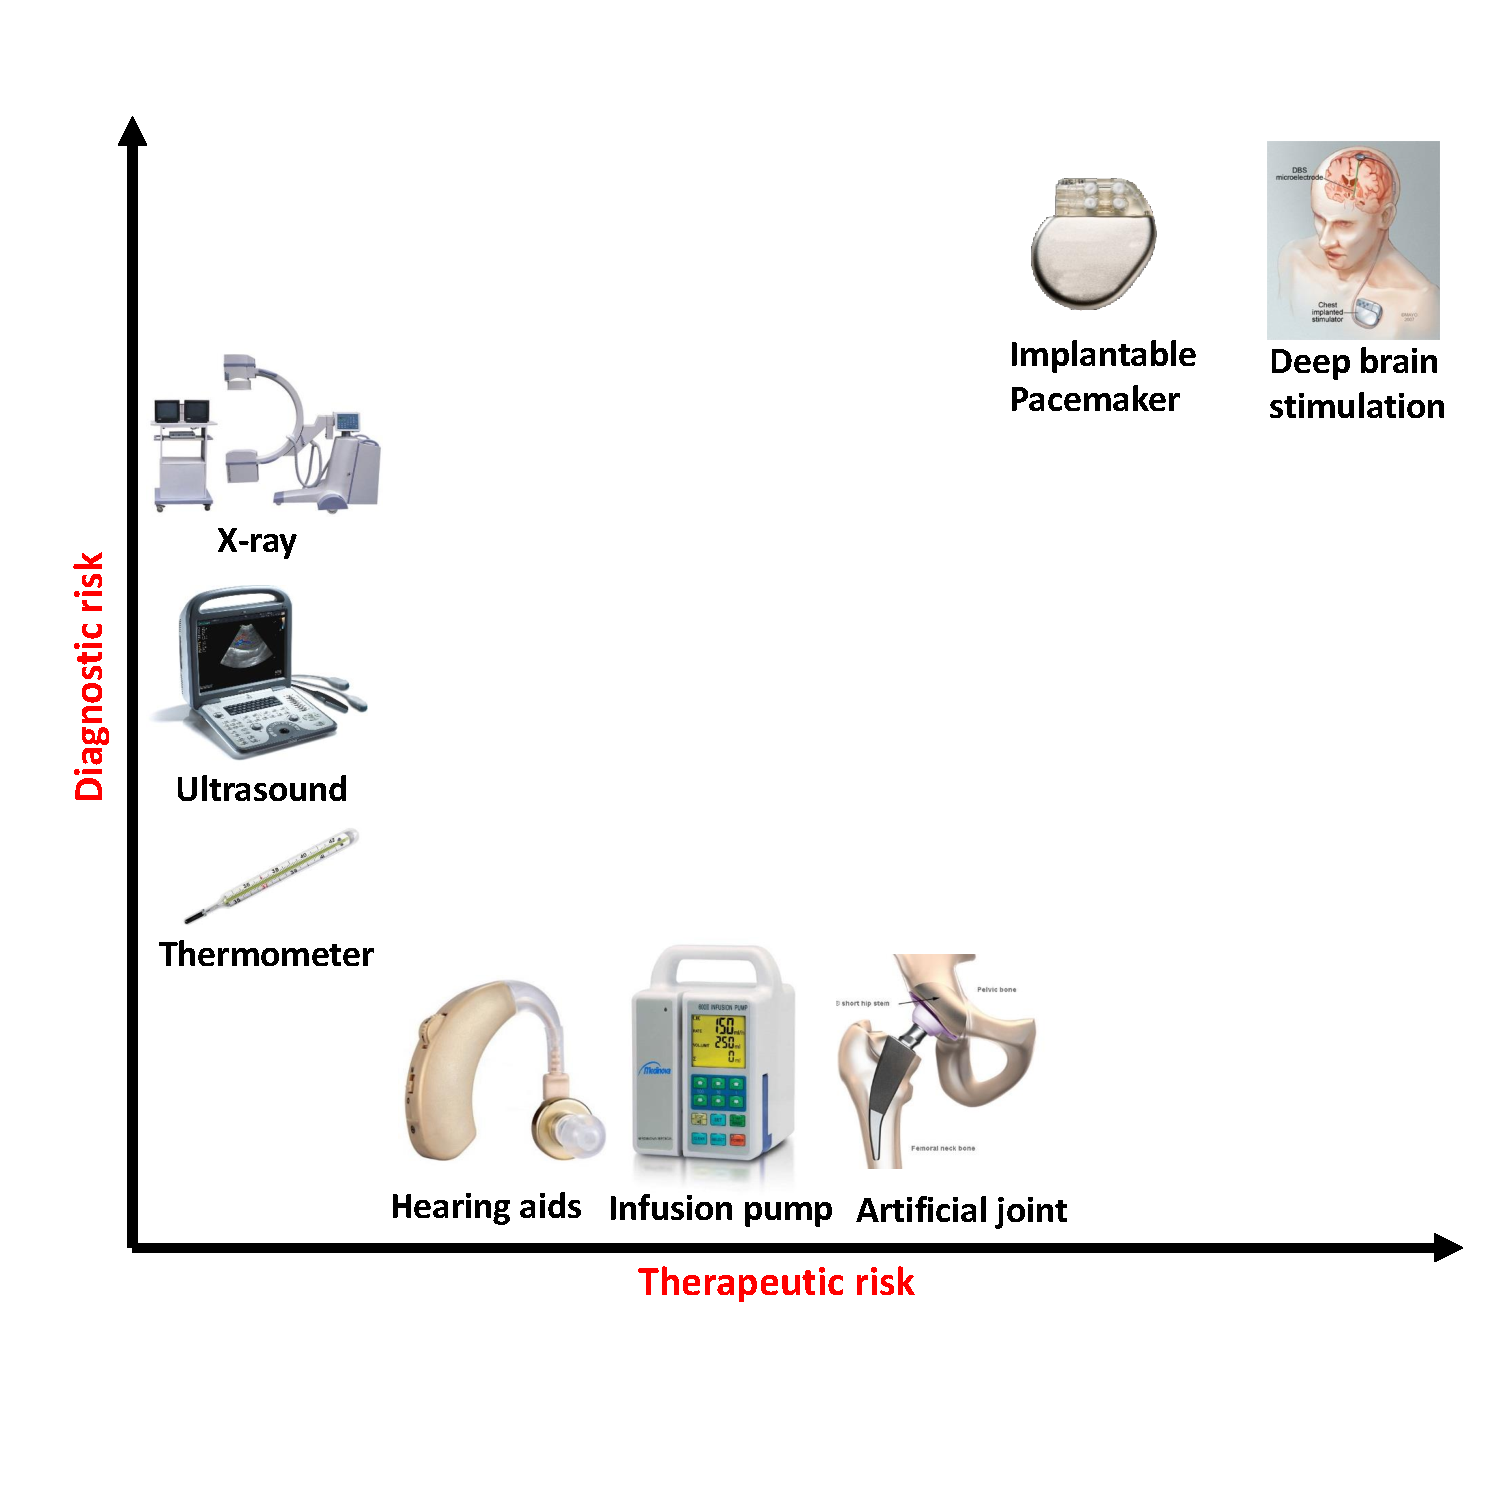
\includegraphics[width=\textwidth]{figs/devices_new.pdf}
		\caption{\small Current medical devices across a range of diagnostic and therapeutic risk. Implantable software-controlled devices such as the pacemaker and defibrillator which operate in a closed-loop of sensing, control and actuation are amongst the highest risk}
		\label{fig:Cur}
\end{figure}

The US Food and Drug Administration (FDA) defines a medical device as an instrument, apparatus, implement, machine, or implant which is:
\begin{itemize}
	\item intended for use in the diagnosis of disease or other conditions, or in the cure, mitigation, treatment, or prevention of disease, in humans or other animals, or
	\item intended to affect the structure or any function of the human body or other animals, and which does not achieve any of its primary intended purposes through chemical action and which is not dependent upon being metabolized for the achievement of any of its primary intended purposes."
\end{itemize}

In general, medical devices are categorized according to their risk factors - Class I, Class II and Class III, corresponding to low-risk, medium-risk and high-risk devices (\cite{class}).  
\figref{Cur} gives an intuitive description of medical devices examples across a range of diagnostic and therapeutic risk.

\begin{figure}[t]
		\centering
		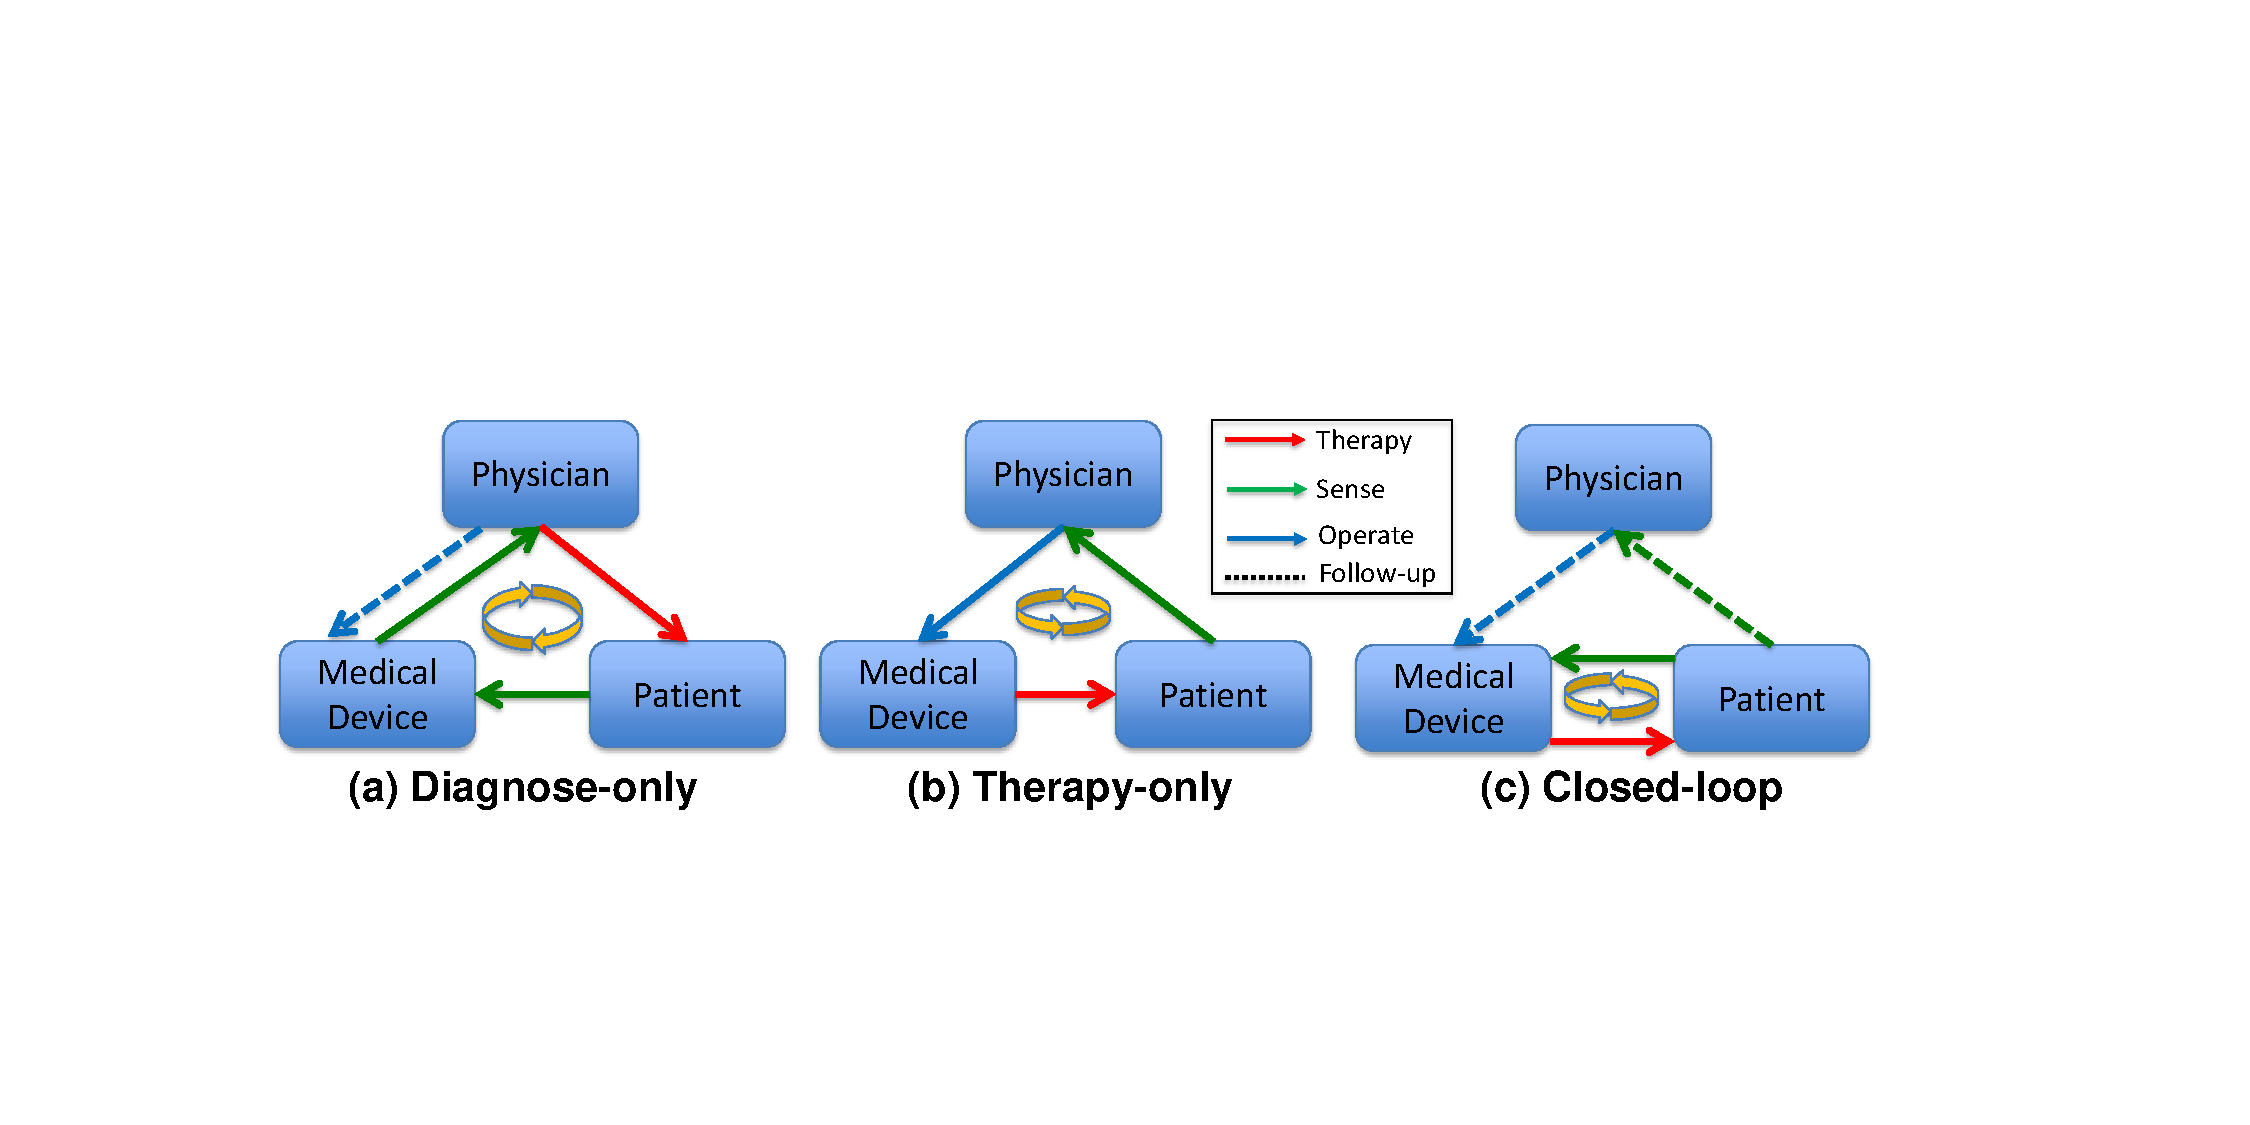
\includegraphics[width=\textwidth]{figs/closed-loop.pdf}
		\caption{\small Diagnostic-only and therapy-only devices do not interact with the patient in direct closed-loop. The physician is responsible for the diagnostic and/or therapeutic decisions. However in closed-loop medical devices, the devices interact with the patient in closed-loop and have to make therapeutic decisions based on their own diagnosis.}
		\label{fig:closed-loop}
\end{figure}

\section{Closing the Device-Patient Loop}
Medical devices operate across a range of invasiveness and intervention with the patient in the loop. 
For diagnostic-only devices, like an X-ray machine, the physician operates the device to obtain patient data. 
Upon interpretation of the data, the physician performs diagnosis followed by delivery of proper therapy to the patient (\figref{closed-loop}.(a)). 
For therapy-only devices, e.g. a drug infusion pump, the physician configures the device infrequently based on prior diagnosis of the patient so the device executes the therapy on the patient (\figref{closed-loop}.(b)). 
We denote these devices as \textbf{Open-loop Medical Devices} as there is no direct feedback loop between the patient and the device. 
For open-loop devices, the device operates under the supervision of professionally-trained physicians. 
The device's safety is mostly determined by how accurately it provides information to the physicians or how faithfully it operates as instructed by the physicians.

There is a class of devices with both diagnostic and therapeutic functions, i.e. implantable cardiac devices to treat cardiac arrhythmia, deep brain stimulation devices (\cite{Brain_sti}) to treat Parkinson's disease and artificial pancreas to treat Type-1 diabetes. 
These devices capture and diagnose the patient's physiological conditions from sensory data, \emph{and} deliver therapy in response (\figref{closed-loop}.(c)). These devices usually operate (semi-) autonomously with very little human intervention. 
We denote them as \textbf{Autonomous Medical Devices}. 
The benefits of autonomous medical devices are timely therapy and better life-style.
However, autonomy of these medical devices also arose safety and efficacy concerns. 
%Malfunctions or inappropriate therapies from these devices also cannot be corrected timely, which can cause serious adverse effects on patients' health. 
With open-loop medical devices, the diagnosis and therapy decisions are made by medical professionals, who have expert knowledge of human physiology. Therefore they are able to identify adverse health conditions and adjust the therapy accordingly. 
On the other hand, closed-loop medical devices have to make both the diagnosis and therapy decisions on their own. 
The domain expertise required to make those decisions has to be programmed into the device. 
It is impossible to encode all the knowledge of human physiology into the device. 
For unanticipated physiological conditions, when the appropriate response has not been programmed into the device, the device may deliver inappropriate therapy which can have an adverse effect on patient's health. 
Therefore, these devices are usually classified into the highest risk category and undergo the most stringent regulation. 
\subsection{Challenges for Developing Autonomous medical Devices}
There are multiple challenges to develop safe and effective autonomous medical devices:

\subsubsection{Physiological Complexity} 
Human physiology is complex and only partially understood. 
For instance, the functionality of the heart can be interpreted from \emph{multiple perspectives}: from its electrical activity, mechanical contractions of the heart muscles, and dynamics of blood flow. 
The physiology of the heart can also be analyzed with \emph{multiple scales}: from the molecular level to cellular level all the way to the organ and system level. 
It is impossible to encode all these contexts into the device, hence inappropriate diagnosis and therapy are observed due to the lack of physiological contexts~\cite{killedbycode, icd_recall}.
	\subsubsection{Physiological Variability}
	Physiological conditions and parameters demonstrate different levels of variability both within the individual at different times, levels of exertion and under the influence of medication and also across individuals. 
	For instance, a segment of the population may have additional electrical conduction pathways within their heart, which makes them vulnerable to certain heart diseases.
	Consequently, autonomous medical devices should be able to safely operate under a large variety of physiological conditions. 
	This is difficult to guarantee, as the device designer must consider all possible physiological conditions, and their interaction with the device, during the development of the device.
	%\hatodoin{last sentence: rather than say "always", say something like: "the designer will likely miss some rare conditions during the design of the device".}
	
	\subsubsection{Limited Observability} 
	Autonomous medical devices normally rely on minimally invasive measurement of the physiological parameters in order to allow the patients to live their normal life. 
	For example, implantable pacemakers and defibrillators commonly have only two leads and therefore two points of observation for the whole heart. 
	The limited observability inevitably leads to ambiguities as different physiological conditions can map to the same input sequence to the device, resulting in inaccurate diagnosis and therapy. 

\subsubsection{Software-related Medical Device Recalls}
The diagnostic and therapeutic functions of the autonomous medical devices are mostly controlled by their software components due to their complexity. 
For instance, implanted cardiac pacemakers and defibrillators have approximately 80,000-100,000 lines of software code which essentially makes all sensing, control and actuation decisions autonomously within the human body, over the 5-7 year device lifetime \footnote{Paul L. Jones. Senior Systems/Software Engineer, Office of Science and Engineering Laboratories, U. S. FDA. Personal communication, 2010.}. 
Software embedded in a medical device, unlike electrical and mechanical components, does not fail due to corrosion, fatigue or have statistical failures of sub-components. 
Software failures are uniquely sourced in the design and development of the system. %Unlike other industries such as consumer electronics where product life cycles are measured in months, software engineering for medical devices often spans a decade and must prioritize safety and efficacy over time to market. 
%\begin{figure}[t]
		%\centering
		%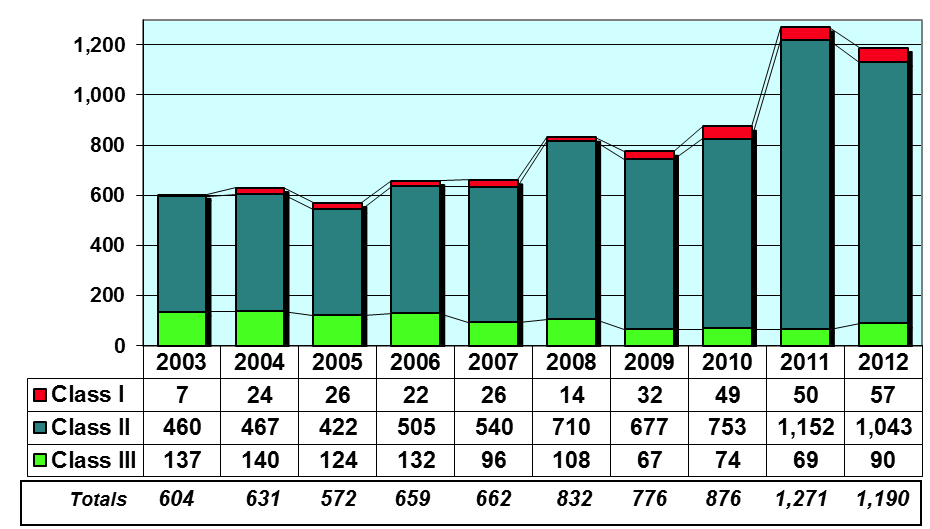
\includegraphics[width=0.8\textwidth]{figs/recalls.jpg}
		%\caption{\small Medical device recalls have risen over the past decade}
		%\label{fig:recalls}
%\end{figure}
\begin{figure}[t]
		\centering
		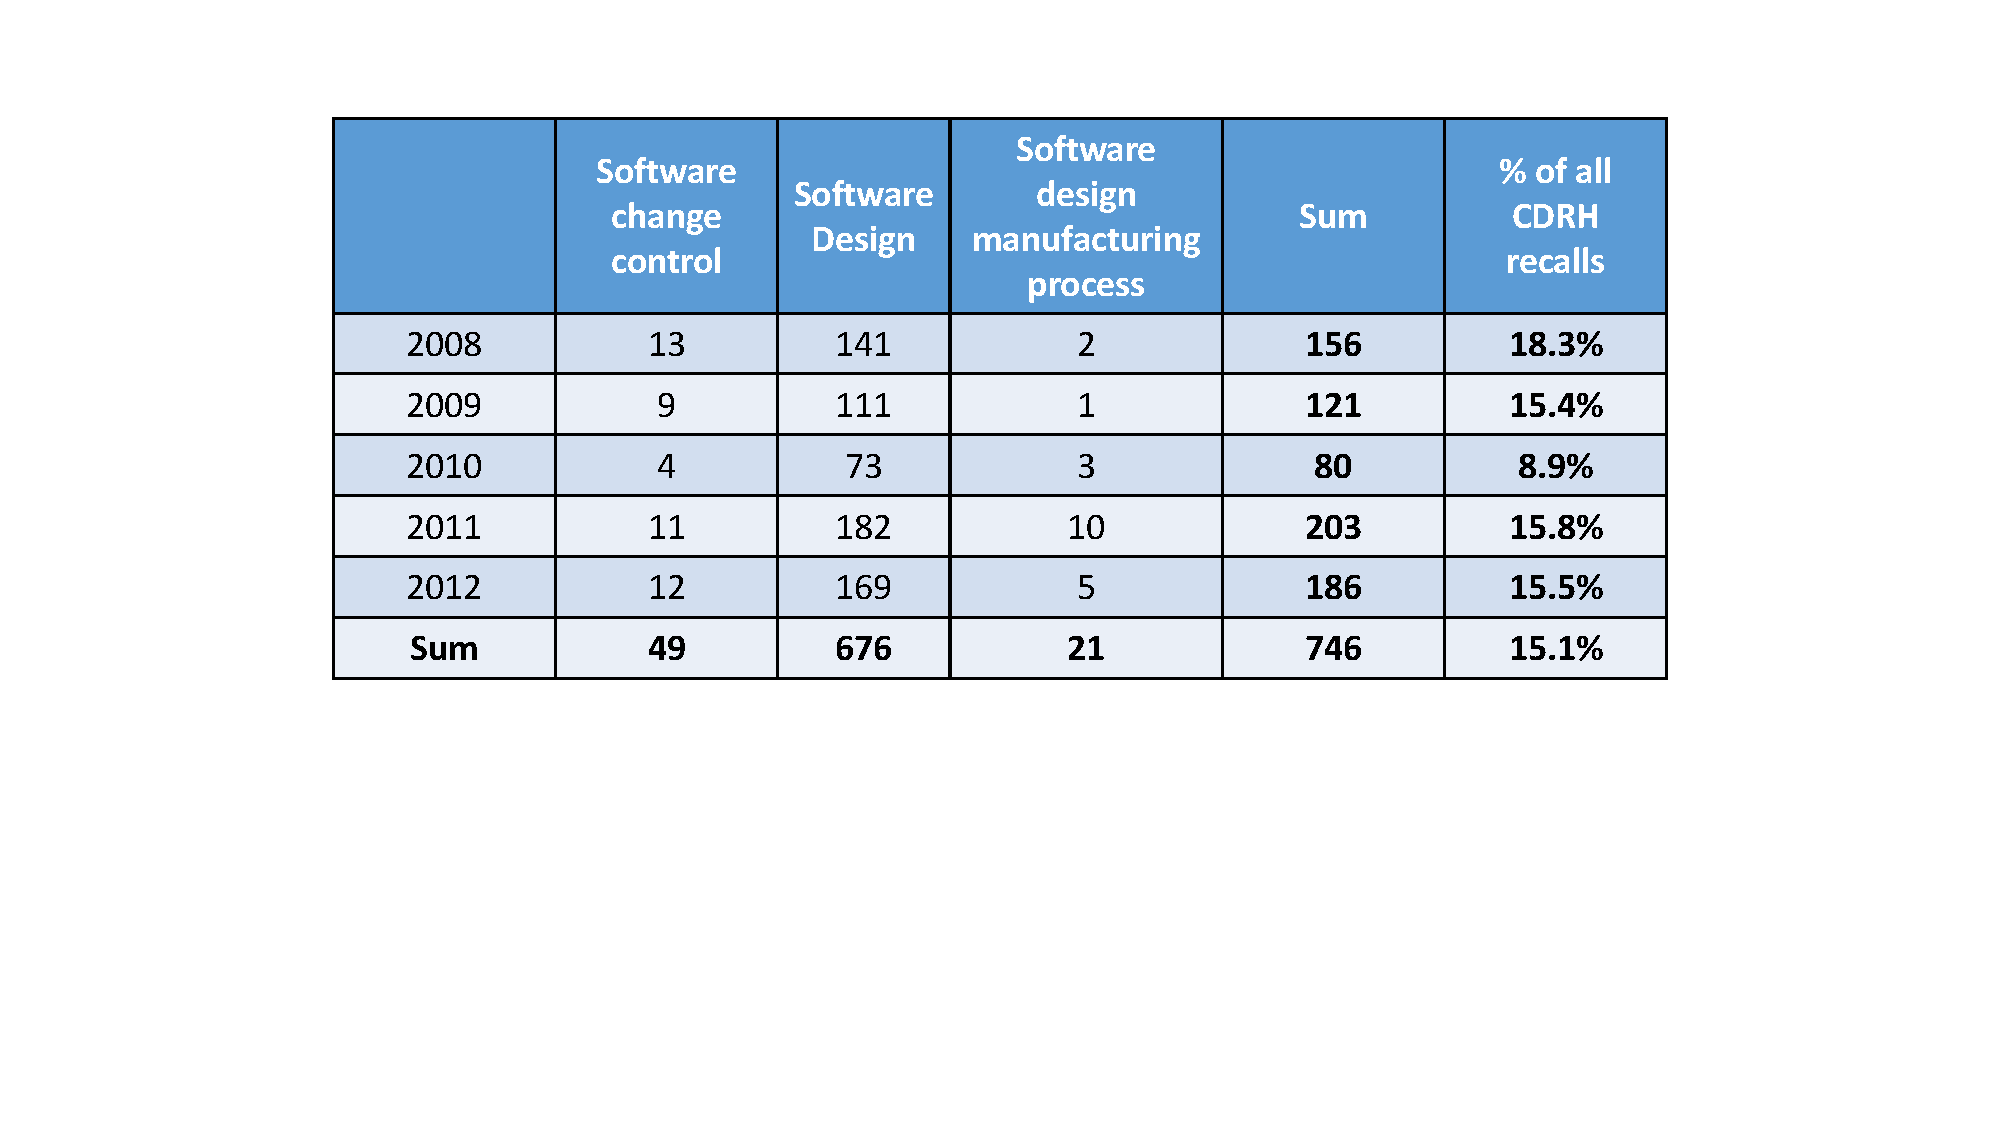
\includegraphics[width=0.8\textwidth]{figs/recalls.pdf}
		\caption{\small Medical device recalls due to software issues have risen from 10\% in the 1990s to \~15\% in the past decade (\cite{recall_rep})}
		\label{fig:soft_recalls}
\end{figure}
%  Over the course of the past four decades, cardiac rhythm management devices such as pacemakers and implantable cardioverter defibrillators (ICD) have grown in complexity and now have more than 80,000 to 100,000 lines of code (\cite{pauljones}). 

According to the US Food and Drug Administration, in 1996, 10\% of all medical device recalls were caused by software-related issues (\cite{medstats}). 
This percentage rose to an average of 15\% of recalls from 2008 to 2012 (\figref{soft_recalls}). 
Malfunctions of closed-loop medical devices usually have severe consequences, which will be categorized as \emph{Class I}, meaning there is a ``reasonable probability that use of these products will cause serious adverse health consequences or death.'' (\cite{medstats2,pacemakerrecalls,killedbycode}). 



\section{Medical Device Regulation Efforts and Challenges}
%The medical device industry is regulated to ensure the safety of the patients and the public. 
In the United States, the FDA is the primary regulatory authority responsible for assuring the \emph{safety, efficacy and security }of patients using medical devices. 
%These three terms can be further elaborated as:
%\begin{itemize}
	%\item \emph{Efficacy}: The device is effective in achieving its intended and expected use.
	%\item \emph{Safety}: The device does not expose the patient, user, or other bystanders to undue risk from its use;
	%\item \emph{Security}: The device has been designed to protect patients, users, and bystanders from both unintentional and malicious misuse of the device
%\end{itemize}
%\begin{itemize}
	%\item Efficacy: The device is effective in achieving its intended and expected use.
	%\item Safety: The device does not expose the patient, user, or other bystanders to undue risk from its use;
	%\item Security: The device has been designed to protect patients, users, and bystanders from both unintentional and malicious misuse of the device
%\end{itemize}
Based on the rationale that 1) manufacturers know their devices better than the regulator, and 2) the variety of medical devices requires a variety of approaches, it is the device manufacturers' responsibility to demonstrate the safety and efficacy of the medical devices. 
Manufacturers are required to complete a pre-market submission before the devices can be released to the market. 
The level of requirements for the submission is determined by the safety classification of the devices.

\subsection{Guidelines During Device Development}
A set of general guidelines are recommended by the FDA (\cite{fda1, fda2, fda3}) which list the activities that need to be performed during the development of the devices. 
In safety-critical industries such as automotive electronics, avionics and nuclear systems, international standards are \textbf{enforced} for software system development, evaluation, manufacturing and post-market changes (\cite{autosar,avsi}). 
This awareness is only beginning to enter the medical device industry as compliance with international standards are "recommended" in the aforementioned guidelines (\cite{formal_fda}). 

\begin{figure}[t]
		\centering
		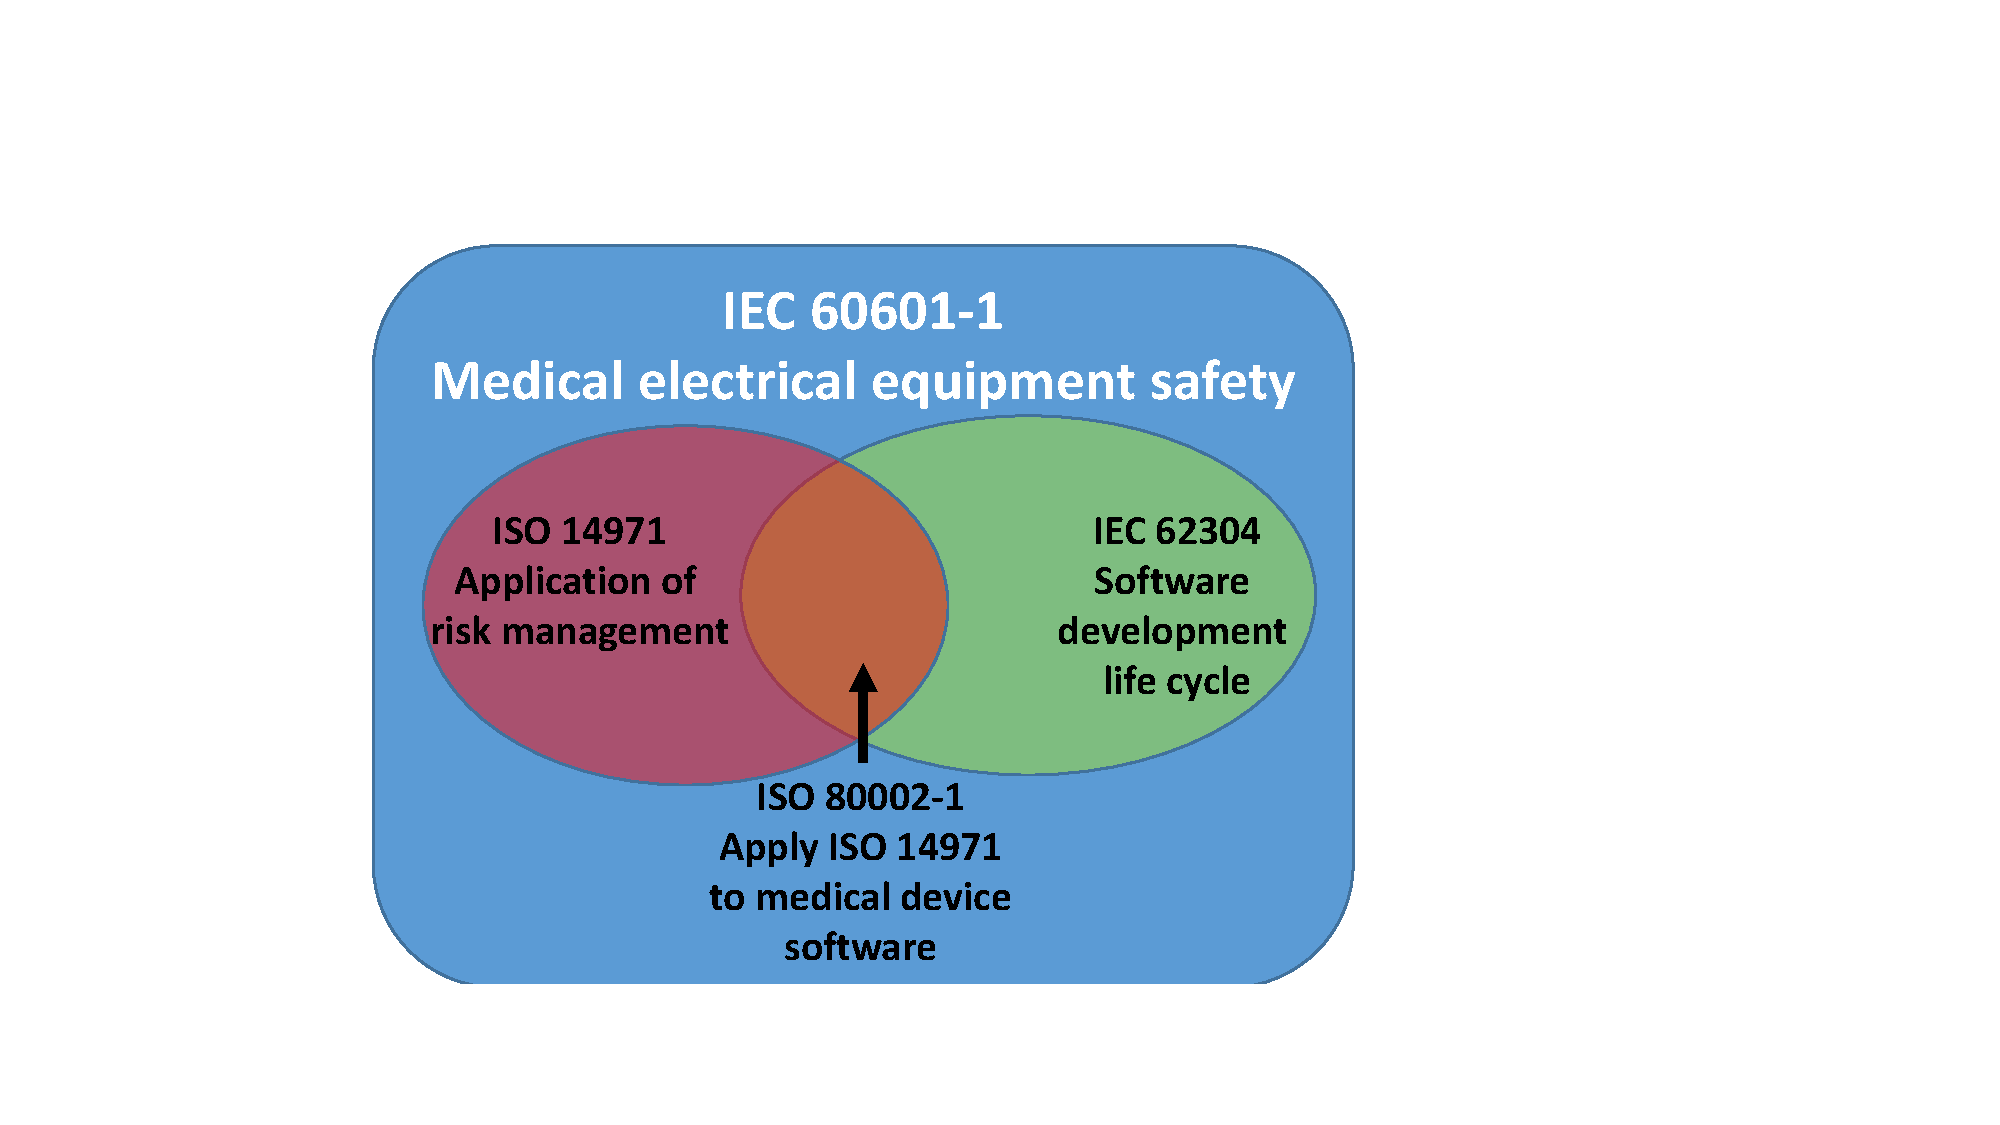
\includegraphics[width=0.6\textwidth]{figs/stardards.pdf}
		\caption{\small International standards for medical device safety. These standards define the required activities during the development process.}
		\label{fig:standards}
\end{figure}

%\subsection{Safety Standards During Development}
\figref{standards} describes the primary standards to enforce medical device safety and their relationships. 
The basic rationale behind these standards is that: if all the risks/hazards of the device are identified and reasonably mitigated, and the device is developed with rigorous process, the device is \emph{reasonably safe}. 
The IEC 60601 Medical Electrical Equipment - General requirements for basic safety and essential performance is a product safety standard that all electronic medical devices must comply to. 
IEC 60324 specifies the processes and activities needed to perform during the software development life cycle to ensure software safety. 

Risk management is a core activity throughout the software development life cycle.
 ISO 14971 is specified for the application of risk management to medical devices. 
In addition, for each risk management activity of ISO 14971, ISO 80002-1 provides additional guidelines for the software component, which highlights and explains approaches to assuring that software safety is adequately addressed.
%%On similar lines, in the European Union there are five medical devices categories based on non-invasive vs. invasive, length of stay in body, contact with blood vessels or the central nervous system, active vs. non-active and implantable devices. (\cite{EU_classify}) 
%%Invasive devices with active interventions are subject to stringent regulations to ensure the patient's safety and efficacy of therapy.
%\begin{figure}[t]
		%\centering
		%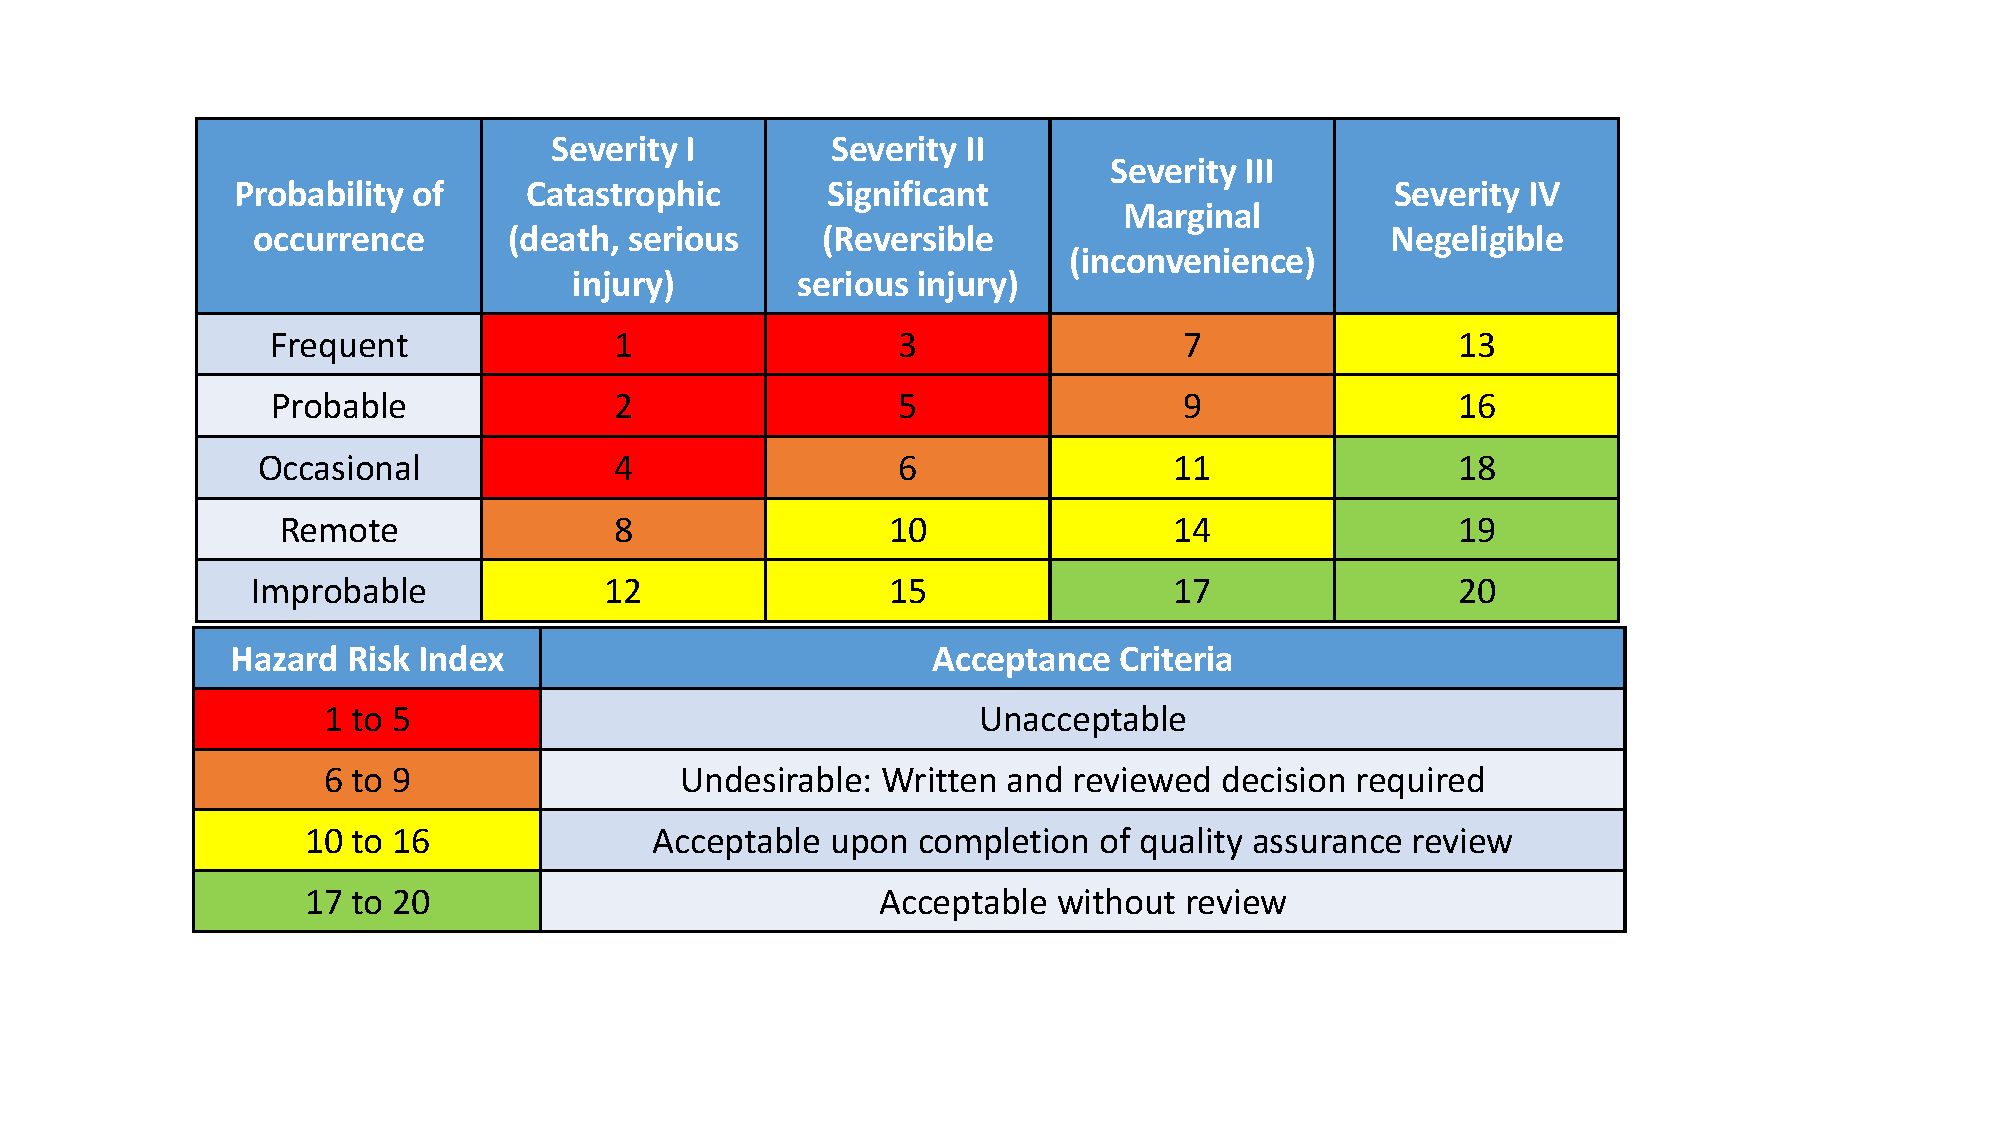
\includegraphics[width=\textwidth]{figs/risk_analysis.pdf}
		%\caption{Top table: Risk index according to occurrence and severity. Bottom table: Risk control using risk index}
		%\label{fig:risk_ana}
%\end{figure}



\subsection{Pre-Market Evaluation with Clinical Trials}
%Regardless of how rigorous the risk management and the device development process are, the devices have to be able to achieve their design goal on the real patient, which can only be evaluated within its physiological environment. 
Devices that have high risk factors are required to submit clinical evidence for their safety and efficacy, often in form of clinical trials. 
In clinical trials, the devices are used on a preselected population of patients following carefully-designed protocols. 
The goal of a medical trial, in part, is to obtain unambiguous results for the primary question of the trial which can support the safety and/or efficacy of the devices. 
However, conducting clinical trials is very time consuming and expensive, and risks found during clinical trials are very expensive to fix (\cite{trialcost}). 

%To address this \textbf{safety gap} between ensuring the device satisfies its therapeutic requirements with the patient-in-the-loop and testing its software specifications, new approaches for closed-loop validation of the device software within the physiological context are needed - this is the primary focus of this article.




%\section{Current Testing, Validation and Verification Approaches}
%In order to facilitate the early detection and correction of any software defects, the FDA has focused on infusion pumps due to the large number of recalls. In April 2010, the FDA began the ``Infusion Pump Improvement Initiative" which offers manufacturers ``the option of submitting the software code used in their infusion pumps for analysis by agency experts prior to premarket review of new or modified devices." 	\cite{}
%
%An effective software verification methodology is therefore needed for the risk analysis and certification of medical device software during the pre-market submission phase. While formal methods of verification are used for medical device software (\cite{challenge, challenge2, challenge3}), testing continues to be required because it can expose different kinds of problems (e.g. compiler bugs), can examine the program in its system context, and increases the diversity of evidence available. Testing for medical device software currently is ad hoc, error prone, and very expensive. Traditional methods of testing do not suffice as the test generation cannot be done independently of the current state of the patient and organ. The primary approach for system-level testing of medical devices is unit testing using a playback of pre-recorded electrogram and electrocardiogram signals (\cite{testing_imd, Vip}). This tests if the input signal triggers a particular response by the pacemaker, but has no means to evaluate if the response was appropriate for the patient condition. Furthermore, this approach of ``tape testing''\Hao{elaborate} is unable to check for safety violations due to inappropriate stimulus by the pacemaker. Pacemaker Mediated Tachycardia (PMT), a condition that is described later in this paper, is a strong example of why we need a model of the heart such as the one presented in this paper, which can be used for closed-loop system analysis. 
%PMT is a condition where the pacemaker inappropriately drives the heart-rate toward the upper rate limit. With a tape test, PMT would not occur and the response of the pacemaker could be classified as appropriate therapy.
%\begin{figure}[t]
		%\centering
		%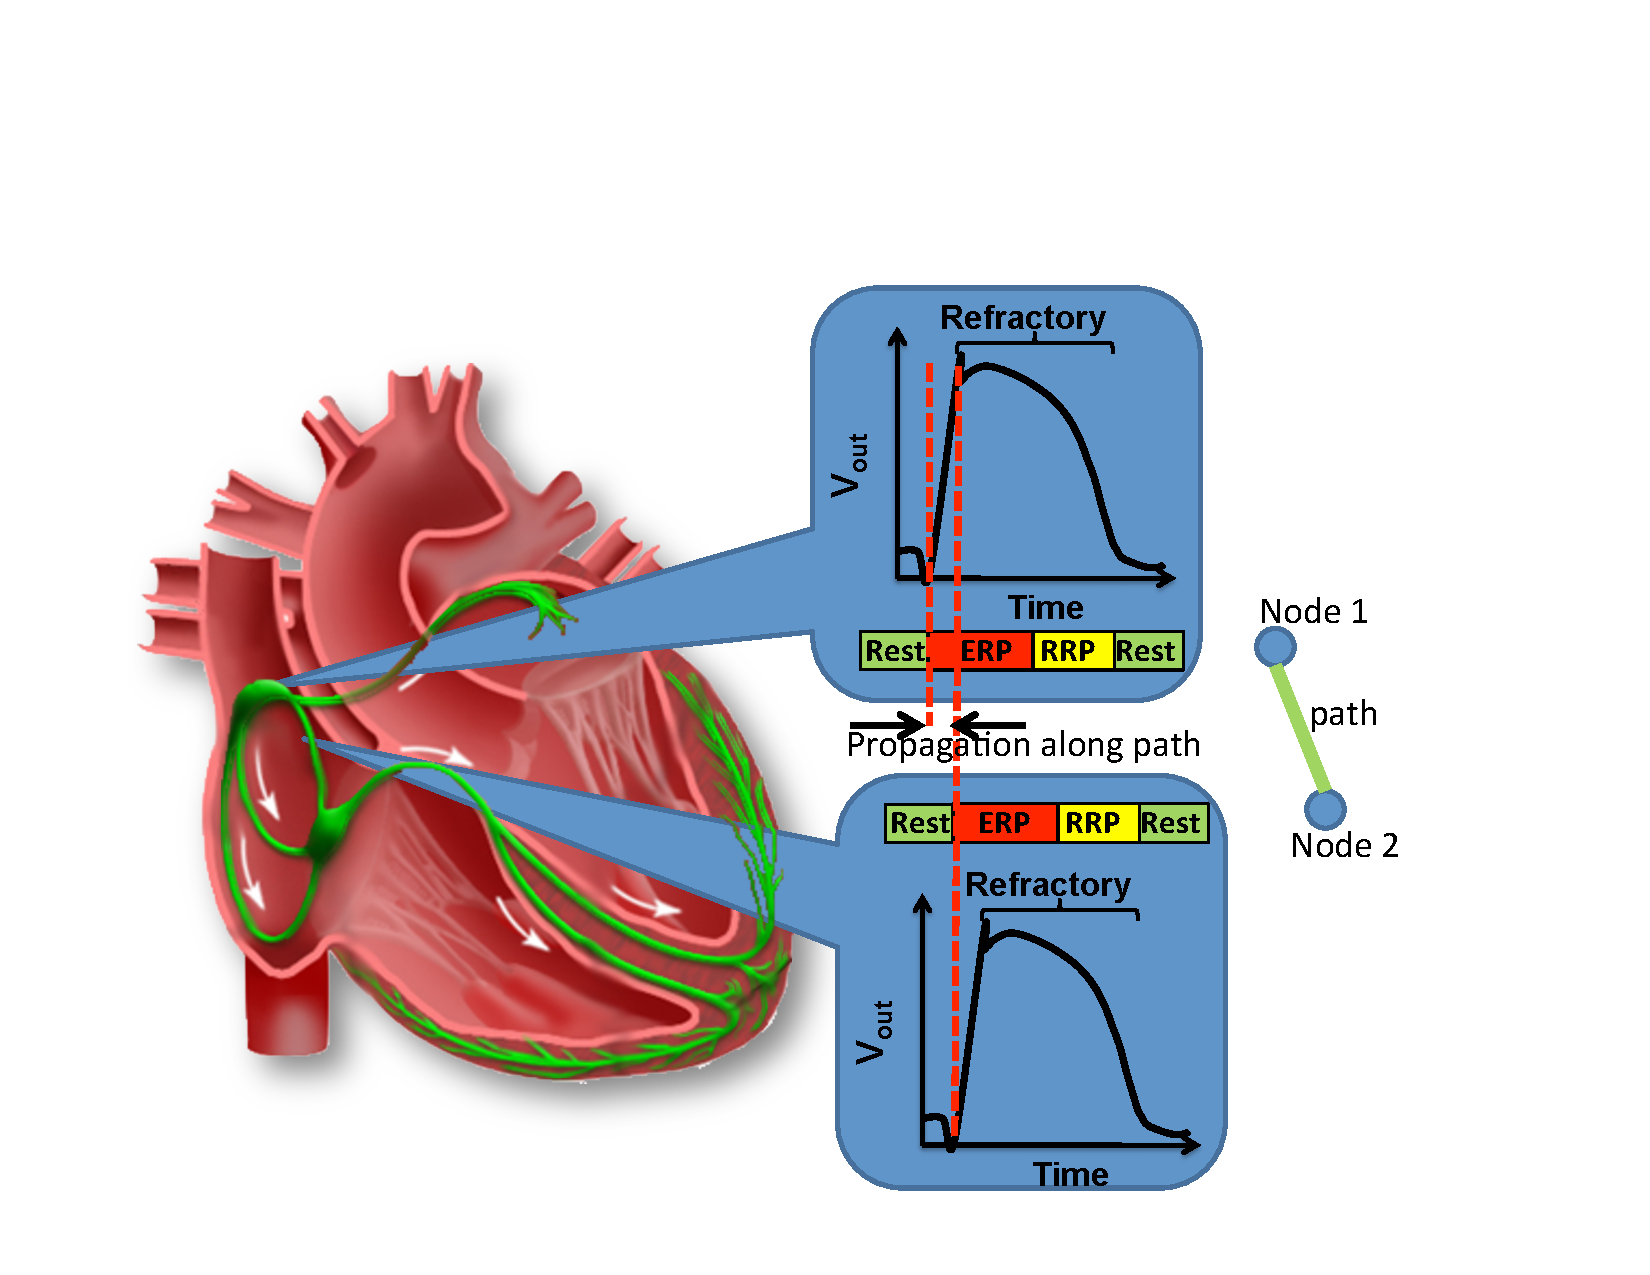
\includegraphics[width=0.8\textwidth]{figs/heartmodel.pdf}
		%%\vspace{-5pt}
		%\caption{\small By extracting timing and electric conduction information we model the signal activation, refractoriness and propagation across the heart tissue as a set of node and path automata.}
		  %%\vspace{-15pt}
		%\label{fig:heartmodel}
%\end{figure}
%As the testing environment (i.e., patient condition) is not entirely under the control of the tester, the problem changes significantly as a degree of nondeterminism is introduced in the process. Implantable medical devices are a primary example of Medical Cyber-Physical Systems where the safety and efficacy of the device and device software must be evaluated within a closed-loop context of the patient. The key challenge is in the generation of physiologically relevant tests such that the device does not provide inappropriate therapy, and does not adversely affect the safety of the patient. In addition, test generation must be interactive and adaptive such that the previous test stimulus affects the current state of the patient. The test generator must consider the current state when generating the next input in a way that advances the purpose of the test. The problem becomes one of the controller synthesis problems and cannot be addressed by an off-the-shelf model checker~\cite{rushby}.  
   %
%Formal methods have traditionally been used for verification of time-critical and safety-critical embedded systems \cite{form-meth}. Until recently, these methods have not been used for medical device certification. \cite{med-form3} presented the use of Extended Finite State Machines for model checking of a resuscitation device. Formal techniques have also been applied to improve medical device protocols (\cite{med-form2}) and safety (\cite{med-form1}), but the authors either used a simplified patient model or did not model the patient at all. 
\subsection{Lack of Closed-loop Validation During and After Device Development}
While formal methods are used for medical device software validation (\cite{challenge, challenge2, challenge3}), testing continues to be the primary method for safety and efficacy evaluation during device development.
Testing for medical device software currently is ad hoc, error prone, and very expensive. 
Traditional methods of testing do not suffice as the test generation cannot be done independently of the current state of the patient and organ. 
The primary approach for system-level testing of medical devices is unit testing using a playback of pre-recorded electrogram and electrocardiogram signals (\cite{testing_imd, Vip}). 
This tests if the input signal triggers a particular response by the device, but is unable to check for safety violations due to inappropriate stimulus by the device. 

The only closed-loop validation activity is clinical trials, which is very expensive and expose the patients to uncertified devices. 
Issues found during clinical trials are also expensive to fix.
There is urgent need for closed-loop validation approaches during and after device development to provide safety and efficacy confidence to the device design.
\section{Model-based Design and Pre-certification of Medical Devices}
%With the deluge of software-based closed-loop medical devices in the coming years, relying on clinical trials as the only closed-loop evaluation method to identify risks rooted in device software is not scalable. 
Model-based design and virtual integration have been proposed and applied in other industries like automotive and avionics (\cite{autosar, avsi}), and can potentially help during the development process and provide extra confidence to the device before conducting clinical trials. 
However, unlike man-made systems like automobiles and aircrafts, physiological systems are less understood with larger variations for the type and degree of patient conditions. 
The lack of faithful models of physiological environment for the autonomous medical devices is one of the reason that model-based approaches are not well-adopted in the medical device industry. 
\begin{figure}[t]
		\centering
		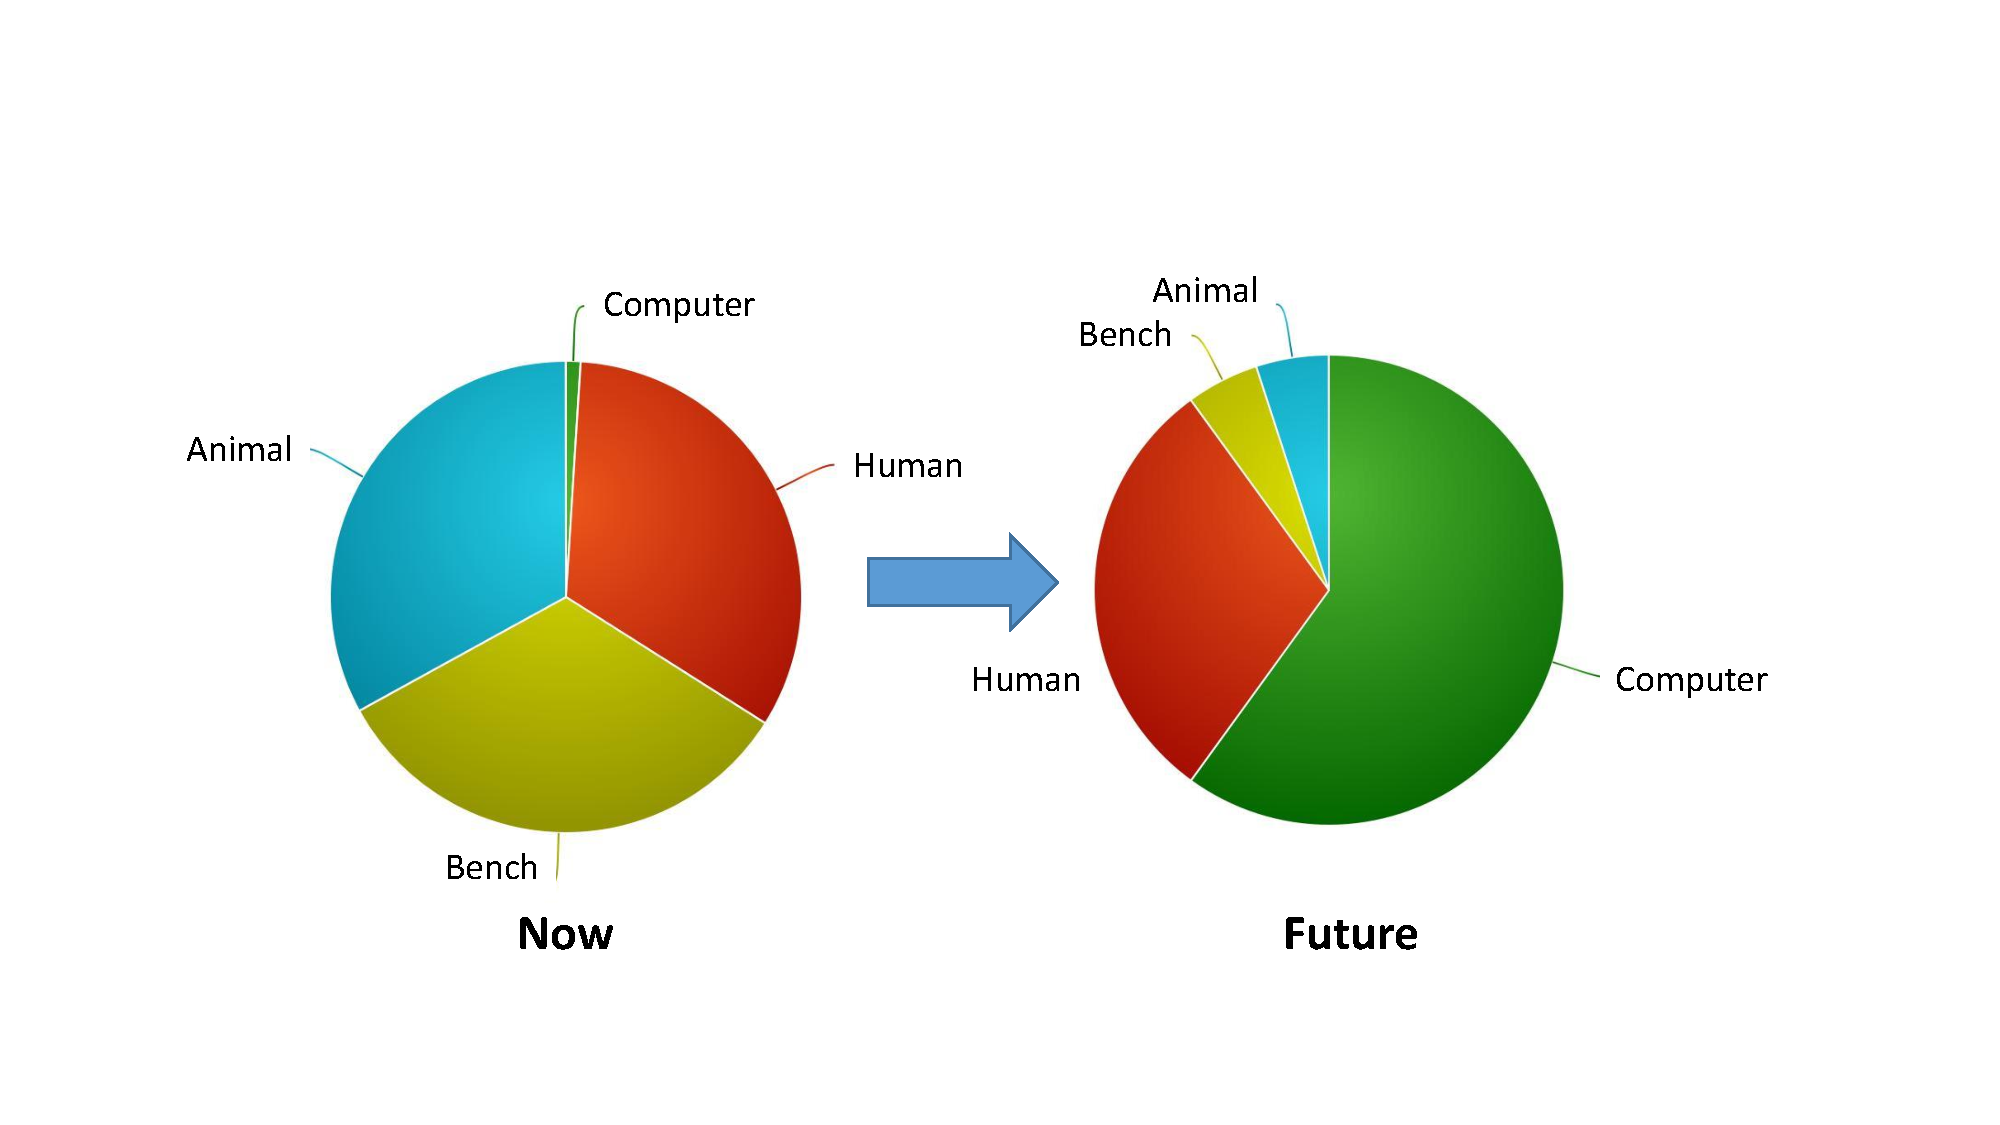
\includegraphics[width=\textwidth]{figs/MDIC.pdf}
		\caption{\small Percentage of computer simulation is expected to increase as safety and effectiveness evidence of medical devices}
		\label{fig:MDIC}
\end{figure}

As computational models of human physiology are developed, they can be used to interact with closed-loop medical devices or their models. 
The FDA is starting to recognize in-silico modeling and simulation as regulatory-grade evidence for device safety and efficacy. 
For example, \cite{pancreas_paul} developed glucose-insulin models that can be used to evaluate control algorithms for artificial pancreas devices which can sense blood glucose and deliver insulin. 
Simulation results with the models have been recognized by FDA to replace animal trials, in part, which significantly reduced cost (\cite{pancreas}). 
With the increasing interest and recognition from the regulators, computer models and simulations are expected to play bigger role as as ``regulatory-grade evidence" evidence in the development of future closed-loop medical devices (\figref{MDIC}).

\section{Contributions}
In this dissertation, implantable cardiac devices are used as working examples to demonstrate how model-based approaches can help improve the safety and efficacy of autonomous medical devices during and after their development. 
By demonstrating the process of developing verified models to generate verified code of the devices, the results of model-based closed-loop validation can provide confidence towards the safety and efficacy of the devices.
\begin{figure}[t]
		\centering
		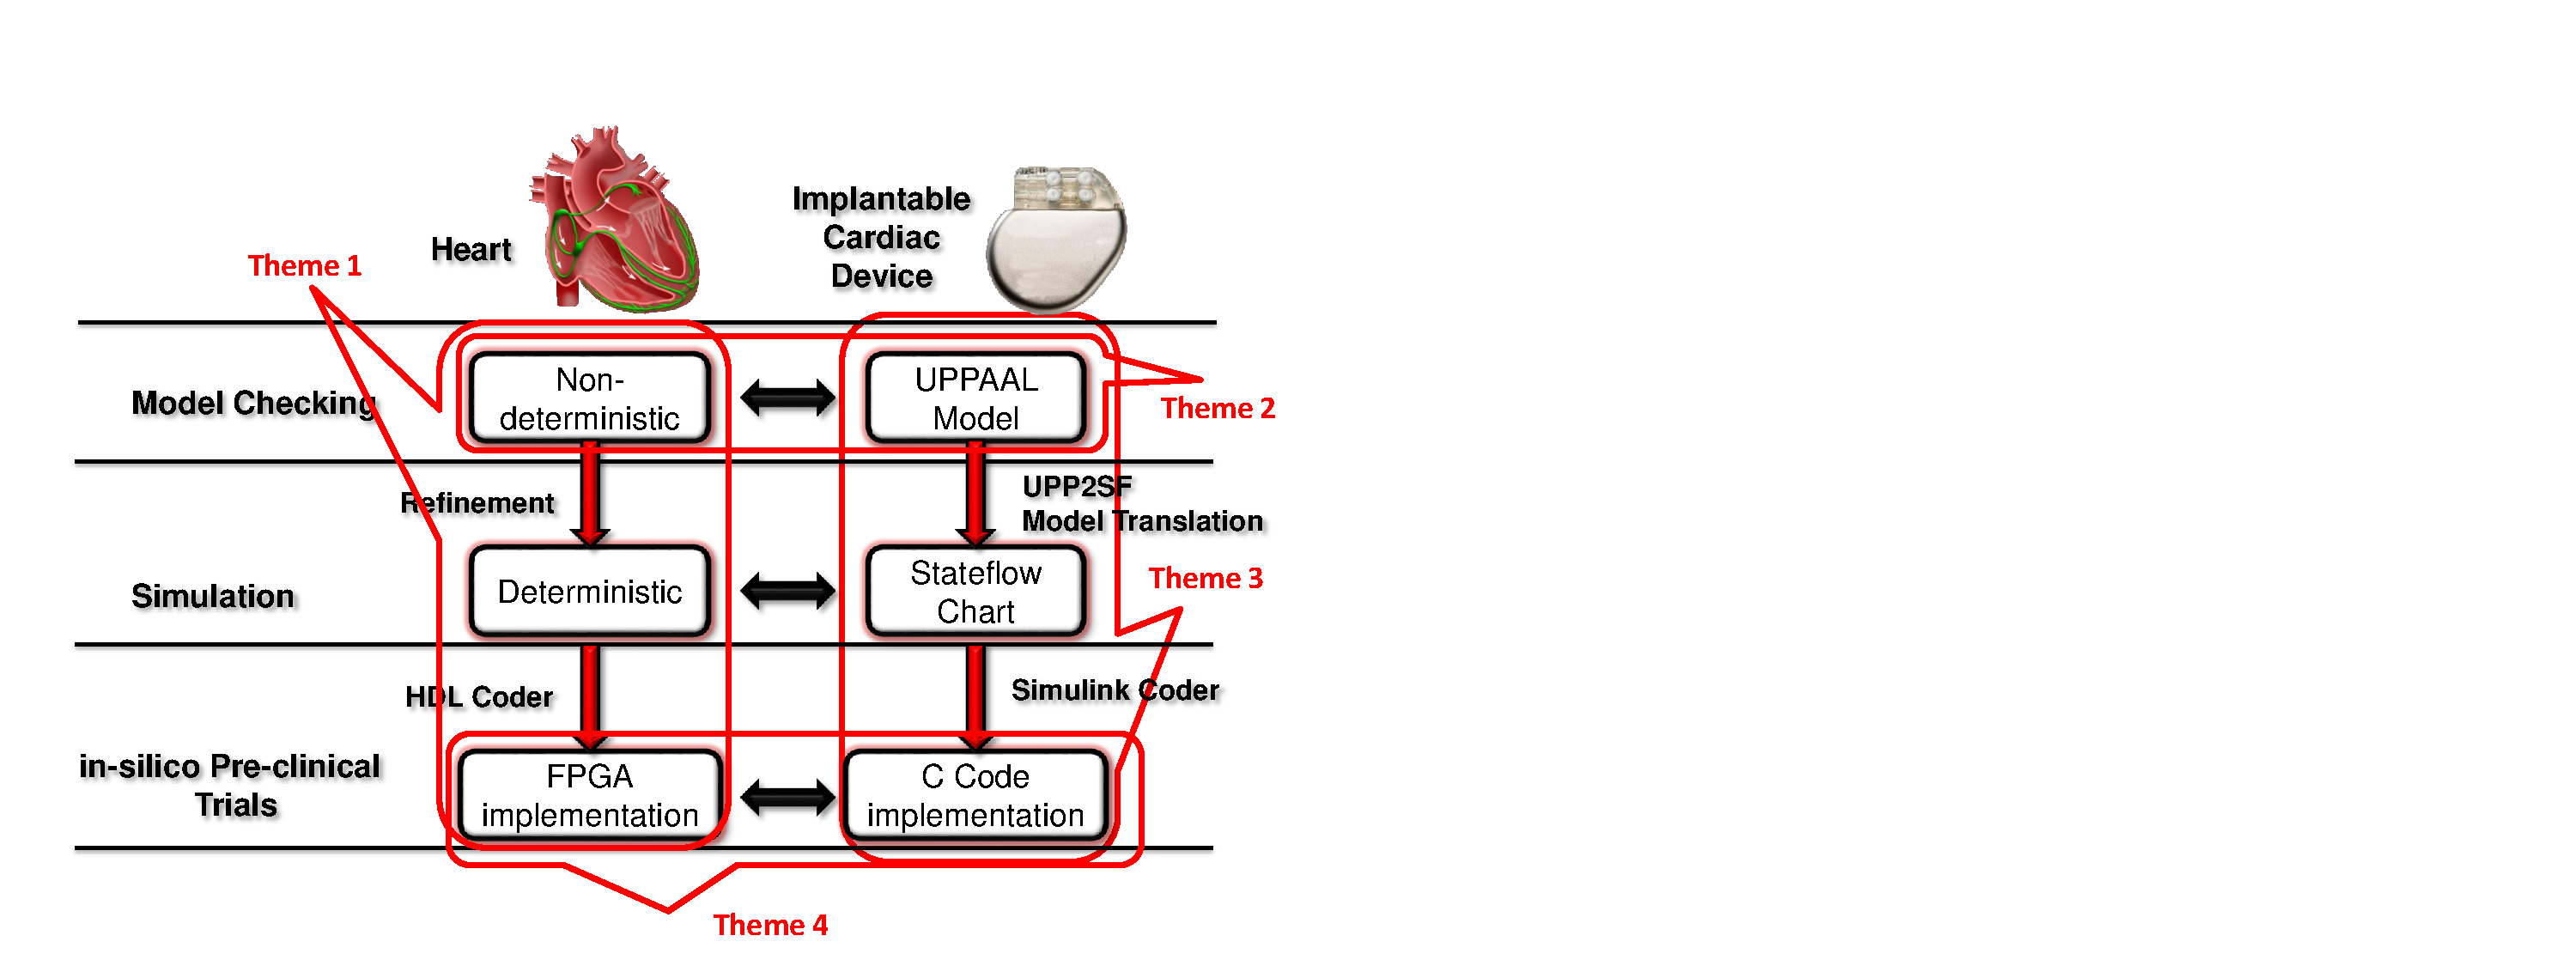
\includegraphics[width=0.8\textwidth]{figs/model_based_b.pdf}
		%\vspace{-5pt}
		\caption{\small Model-driven design for verified models to verified code for the closed-loop heart and pacemaker system}
		  %\vspace{-15pt}
		\label{fig:modeling_overview}
\end{figure}

Fig. \ref{fig:modeling_overview} demonstrates the structure of the dissertation.
The dissertation can be broken down into 4 themes, which are illustrated in \figref{modeling_overview}. 

The remaining dissertation is arranged as follow:
Chapter 2 discusses a dual chamber pacemaker design (\cite{compass}) as the motivating example to illustrate the safety hazards that the device may pose to the patients.
Chapter 3 discusses the physiological models that are necessary for closed-loop evaluation of medical devices, and how to use those models to represent complex physiology with large variability \cite{VHM_proc}.
Chapter 4 discusses the use of model-checking techniques to evaluate the safety and efficacy of device design early in the device design stage, with focus on the abstraction and refinement of the heart models to cover large variety of physiological conditions (\cite{STTT13}).
Chapter 5 discusses the rigorous translation from verified device model to device implementation which maintains the verified properties (\cite{RTAS12}).
Chapter 6 discusses the in-silico pre-clinical trial, which the devices are evaluated on a virtual patient cohort consists of physiological models to provide useful insights for planning a clinical trial. 

%The contribution of this effort is three-fold: (a) We developed an integrated functional (i.e., clinically-relevant) and formal (i.e., timed automata based) Virtual Heart Model  (VHM) (see \figref{heartmodel}) and a pacemaker device model for interactive and clinically relevant test generation.  (b) We provide a set of general and patient condition-specific pacemaker software requirements to ensure the safety of the patient is met under all cases, and (c) We provide a means to test and verify the closed-loop system over a variety of basic operation tests where the heart rate must be maintained, the atrial-ventricle synchrony must be enforced and complex closed-loop tests, where the pacemaker must not initiate tachycardia or perform improperly during lead displacement. With this approach of model-based testing, an executable functional model of the pacemaker is created at an early stage in the development process. This model-based methodology is an early step in addressing the urgent need for pre-market evaluation of medical device design and certification.

\section{Useful terminologies for often misinterpreted terms}
Ensuring the safety and efficacy of complex medical devices has drawn interest not only from stakeholders like regulators and industries, but also medical professionals and academia. 
Different communities have different interpretations over certain terminologies, often causing misunderstandings. 
In this dissertation, terminologies from the regulation perspective are adopted. 
Most of the definitions are referred from the FDA guideline document General Principles of Software Validation (\cite{fda2}). 
Below are several terminologies that are used throughout the dissertation which worth clarifying.
\subsection{Requirements vs. Specifications}
By the definition of the FDA (\cite{fda3}), the requirements of a system describe \textbf{what} the system should achieve and the specifications of a system describe \textbf{how} the system is designed to satisfy the requirements. 
For instance, a requirement for an autonomous car is "The car should not hit objects". 
The corresponding specification can be "brake if the speed of the car is greater than $x$ and the distance to the object is less than $y$". 
It is obvious that a car satisfying its specification may not satisfy the requirement (e.g. when the car is driving too fast or the obstacle pops up right in front of the car). 
In this dissertation, the word requirement in particular denotes the intended uses of the medical devices to improve physiological conditions.

\subsection{Validation vs. Verification vs. Testing}
As defined in \cite{fda2}, software validation is the confirmation by examination and provision of objective evidence that:
\begin{enumerate}
	\item software specifications conform to user needs and intended uses, and 
	\item the particular requirements implemented through software can be consistently fulfilled
\end{enumerate}
The first aspect ensures the device is safe and effective. 
The second aspect maintains the traceability of requirements throughout the development life cycle.
Software verification fulfills the second aspect of software validation by "providing objective evidence that the design outputs of a particular phase of the software development life cycle meet all of the specified requirements for that phase. "
\begin{figure}[t]
		\centering
		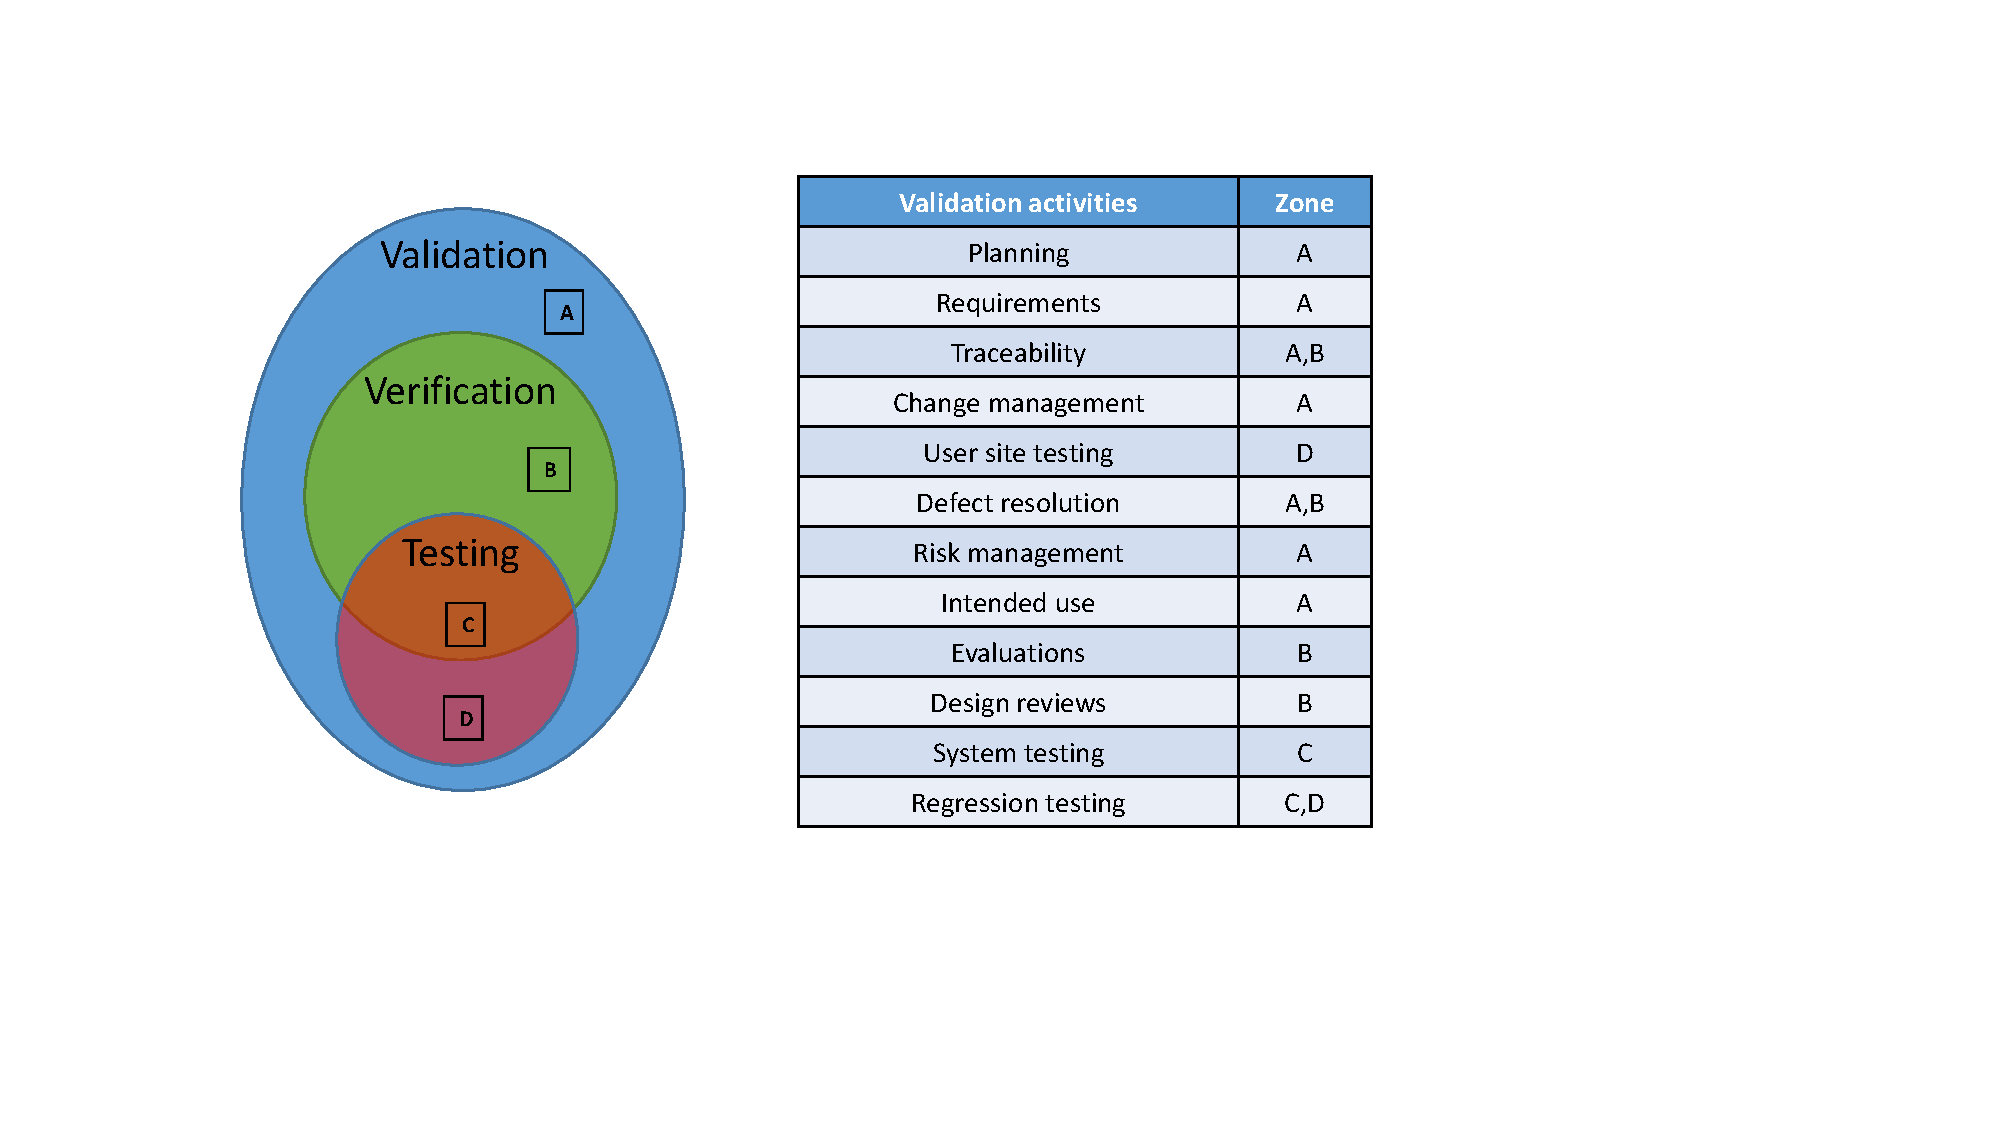
\includegraphics[width=\textwidth]{figs/validation.pdf}
		\caption{Validation activities during the software development life cycle (\cite{Vogel})}
		\label{fig:validation}
\end{figure}

Testing is the technique that can be used for validation and/or verification. \figref{validation} illustrates the relationship between validation, verification and testing, and different activities during the software development life cycle to ensure the safety and effectiveness of the software.
\subsection{Closed-loop vs. Open-loop Evaluation}
In open-loop evaluation, i.e. open-loop testing, input sequences are send to the system and system outputs are compared with expected outputs. 
In open-loop testing, the system outputs do not affect the inputs afterward. 
In closed-loop evaluation, the environment of the system is taken into account. 
System outputs affect the state of the environment and thus affect the input sequences. 
For closed-loop medical devices, clinical trials are currently the most common closed-loop evaluation method. 
Enabling closed-loop evaluation during device design requires models of the environment, which is human physiology for closed-loop medical devices.

Closed-loop evaluation accomplishes two goals in model-based design: 1) It enforces environmental constraints so that the test space is smaller and the test cases have physiological relevance, 2) Execution traces can be better interpreted as the physiological models encode domain knowledge. 
%%Through each of the chapters to follow, we cover different aspects of modeling the physiological system and the device, validating the models, running model checking on the closed-loop system and testing the deterministic systems derived from the abstract models. With the goal of 

%%The US Food and Drug Administration defines medical device an instrument, apparatus, implement, machine, contrivance, implant, in vitro reagent, or other similar or related article, including a component part, or accessory which is:
%%\begin{itemize}
%%	\item recognized in the official National Formulary, or the United States Pharmacopoeia, or any supplement to them
%%	\item intended for use in the diagnosis of disease or other conditions, or in the cure, mitigation, treatment, or prevention of disease, in man or other animals, or
%%	\item intended to affect the structure or any function of the body of man or other animals, and which does not achieve any of its primary intended purposes through chemical action within or on the body of man or other animals and which is not dependent upon being metabolized for the achievement of any of its primary intended purposes."
%%\end{itemize}
\chapter{A Motivating Example: A Dual Chamber Pacemaker Design}
Intuitively, an autonomous medical device like pacemaker should satisfy the following requirements: 1) improve unhealthy physiological conditions of a patient (efficacy), and 2) not to deteriorate current physiological condition (safety).
Evaluating both requirements requires understanding of the physiological environment the device is in.
In the following sections, the physiological basis for the heart and the pacemaker is introduced, followed by a dual chamber pacemaker specification \cite{compass}.
Potential safety hazards for a pacemaker were then analyzed and two known safety hazards were discussed in detail.
The dual chamber pacemaker specification is then used throughout the thesis to demonstrate how different model-based techniques can be used to validate the safety and efficacy of an autonomous medical device.
\section{Physiology Basis of the Heart and the Pacemaker}
First, we use this small section to introduce the physiology basis of the heart and the application of implantable cardiac devices. 
Readers with knowledge of this subject can skip to the following sections.
\subsection{Blood Circulation System}
The heart is the "motor" for blood circulation within our body. The heart has two ventricles which pump the blood out of the heart, and two atria which gather blood from the body and pump them into the ventricles. (\figref{circulation}.(a)) There are two circulations through the heart: the \emph{Pulmonary circulation} and the \emph{Stemic circulation}. In the pulmonary circulation, the right atrium collects oxygen-depleted blood from all over the body and pumps it into the right ventricle. The right ventricle then pumps low-oxygen blood to the lungs. The blood gets oxygenated in the lungs and gathers into the left ventricle. In the stemic circulation, the oxygenated blood in the left atrium is pumped into the left ventricle. The left ventricle pumps the blood to the rest of the body and the heart itself. After the body extracts the oxygen from the blood and injects carbon dioxide, the oxygen-depleted blood then flows back to the right atrium.
\begin{figure}[!t]
\centering
		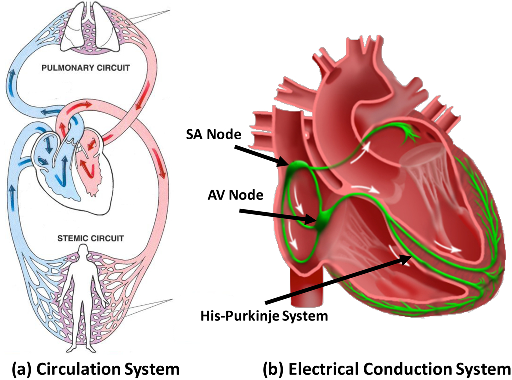
\includegraphics[width=0.9\textwidth]{figs/circulation.pdf}
		
%\vspace{-10pt}
\caption{\small (a) The circulation system. (b) Electrical Conduction system of the heart}
\label{fig:circulation}
%\vspace{-15pt}
\end{figure} 
\subsection{Electrical Conduction System of the Heart}
The oxygen demand of the body changes during different activities. For example, the demand is higher while running and lower while sleeping. To satisfy these demands, the heart muscles in the atria and the ventricles have to contract with certain pattern and frequency in accordance to optimize the \emph{Cardiac Output}, which refers to the volume of blood pumped by the heart per minute (mL blood/min). The coordinated contractions of the heart muscles are governed by the electrical conduction system of the heart (\figref{circulation}.(b)) A \emph{Normal Sinus Rhythm (NSR)} is the healthy heart rhythm which provides efficient blood flow. During a NSR, electrical signals are periodically generated by the \emph{Sinoatrial (SA) node} in the upper right atrium, which acts as the intrinsic pacemaker of the heart. The signals conduct throughout both atria and trigger muscle contractions to push blood into the ventricles. After a long conduction delay at the \emph{AV node} so that both ventricles are fully filled, the signals conduct through fast-conducting \emph{His-Purkinje} system to trigger almost simultaneous contractions of the ventricles and pump blood out of the ventricles. 

Derangement from NSR can result in insufficient cardiac output and thus insufficient oxygen supply to the body and/or the heart itself, which are referred to as \emph{Arrythmia}. Arrhythmia impair the heart's ability to efficiently pump blood and compromise the patient's health. 
Arrhythmia are categorized into so-called \emph{Tachycardia} and \emph{Bradycardia}. Tachycardia features undesirable fast heart rate which can cause inefficient blood pumping. Bradycardia features slow heart rate which results in insufficient blood supply. Bradycardia are due to failure of impulse generation with anomalies in the SA node, or failure of impulse propagation where the conduction from atria to the ventricles is delayed or blocked. 
\subsection{Electrophysiology and Implantable Cardiac Devices}
\label{EP}
The electrical activities of the heart closely couple with the mechanical contractions thus the electrical activities of the heart can be monitored and used to diagnose arrhythmia. The most well-known method is Electrocardiogram (ECG), which measures the integration of electrical activities of the heart measured along different axis on the body surface. The electrical activities can also be directly measured by inserting electrodes through the vein into the heart. The electrodes are placed against the inside heart wall and localized electrical activities can be measured. Physicians can also deliver pacing sequence through the electrodes to explore the heart conditions. This procedure is referred to as Electrophysiological (EP) Testing  (\cite{josephson}) and the signals are referred to as electrograms (EGMs) (\figref{probes}.b). The timing and morphology of the  ECG and EGM signals together are used to diagnose arrhythmia.
\begin{figure}[!t]
\centering
		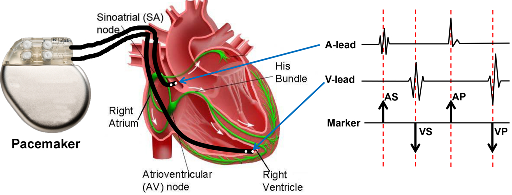
\includegraphics[width=0.9\textwidth]{figs/egm.pdf}
		
%\vspace{-10pt}
\caption{\small (a) Lead placement for a dual chamber pacemaker. (b) Electrogram (EGM) signals measured from pacemaker leads and corresponding internal pacemaker events}
\label{fig:probes}
%\vspace{-15pt}
\end{figure} 

%Implantable pacemakers follow the principle of EP testing. For a dual chamber pacemaker, two leads are inserted into the right atrium and right ventricle, respectively. The pacemaker senses the intrinsic generation and conduction of the electrical signals in the two chambers and deliver electrical pacing when the heart rate and/or atria-to-ventricles conduction interval are abnormal.
The implantable cardiac pacemakers are rhythm management devices designed to treat bradycardia. A typical dual chamber pacemaker has two leads inserted into the heart through the veins which can measure the local electrical activity of the right atrium and right ventricle respectively (\figref{probes}.a). According to the timing between sensed impulses, the pacemaker may deliver electrical pacing to the corresponding chamber to maintain proper heart rhythm.

\section{A Dual Chamber Pacemaker Specification}
The focus of this section is implantable pacemaker, which is one of the simpler implantable cardiac devices.
%The functionality of a pacemaker is based on the timing and patterns of local electrical events. 
The specifications are based on the algorithm descriptions from Boston Scientific manuals (\cite{compass}) and the functional description released as part of the Pacemaker Challenge (\cite{challenge}). 


The pacemaker is designed for patients with bradycardia (i.e. slow heart rate). 
Two leads, one in the right atrium and one in the right ventricle, are inserted into the heart and fixed onto the inner wall of the heart. 
These two leads monitors the local activation of the atria and the ventricles, and generate corresponding sensed events \textsf{(AS, VS)} to its software. 
The software determines the heart condition by measuring time difference between events and delivers pacing events \textsf{(AP, VP)} to the analog circuit when necessary. 
The analog circuit then delivers pacing signals to the heart to maintain heart rate and A-V synchrony. 
In order to deal with different heart condition, pacemakers are able to operate in different modes. 
The modes are labeled using a three character system (e.g. $xyz$). 
The first position describes the pacing locations, the second location describes the sensing locations, and the third position describes how the pacemaker software responds to sensing. 
Here we introduce the widely used DDD mode pacemaker which is a dual chamber mode with sensing and pacing in both atrium and ventricle. 

\begin{figure}[!b]
\center
%\vspace{-10pt}
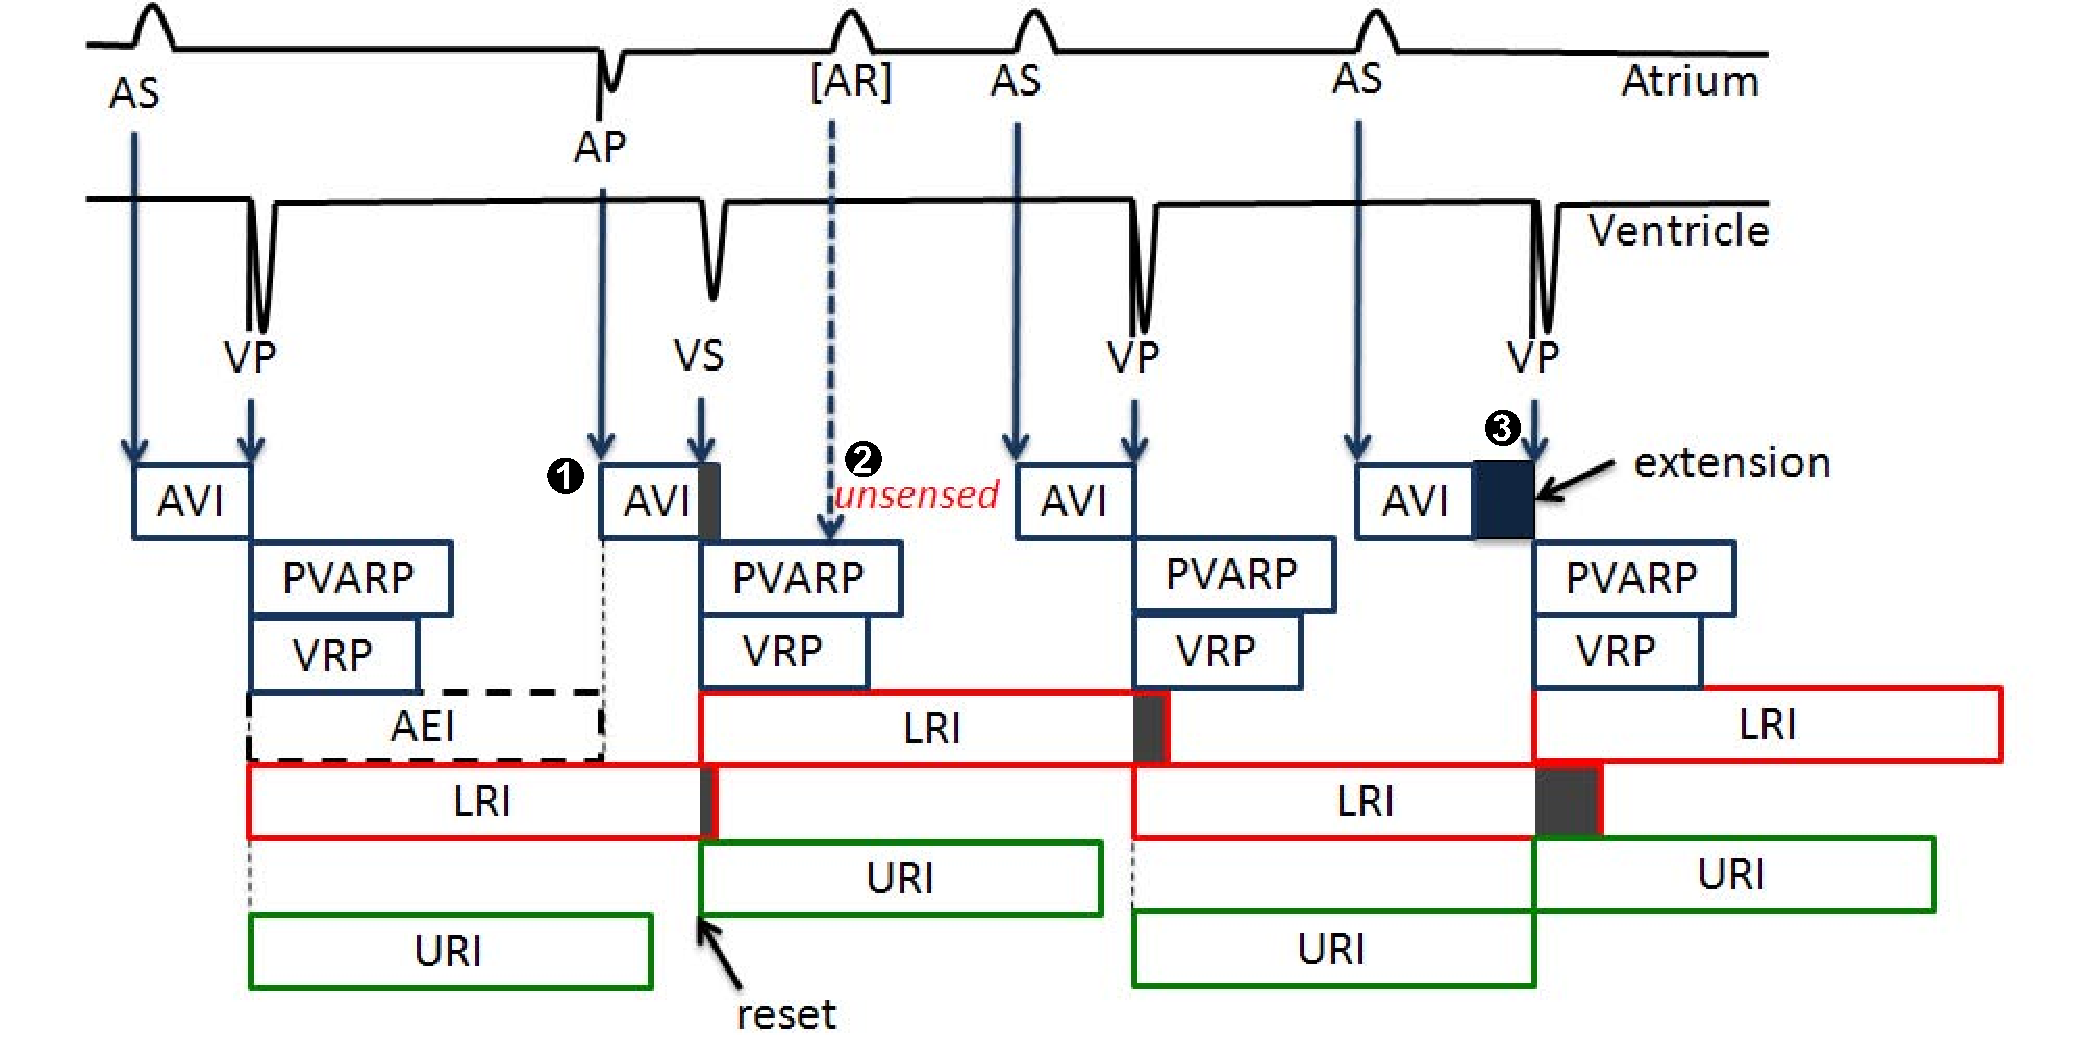
\includegraphics[width=0.85\textwidth]{figs/PM_timers.pdf}
%\vspace{-10pt}
\caption{Basic 5 timing cycles for a dual chamber pacemaker which include the Lower Rate Interval (LRI),  Atrio-Ventricular Interval (AVI), and Upper Rate Interval (URI). Also included are the blanking intervals, Post Ventricular Atrial Refractory Period (PVARP) and Ventricular Refractory Period (VRP), to inhabit action by the pacemaker.}
\label{fig:PMtimers}
%\vspace{-10pt}t

\end{figure} 
A DDD pacemaker has five basic timing cycles triggered by external and internal events, as shown in \figref{PMtimers}. 

\subsubsection{Lower Rate Interval (LRI)}
%\vspace{-5pt}
The Lower Rate Interval (LRI) defines the longest interval allowed between two ventricular events, thus keeping the heart rate above a minimum value. 
In DDD mode, the LRI interval is divided into a V-A interval (TLRI-TAVI) and a A-V interval (TAVI). 
Since the last ventricular event \textsf{(VS, VP)}, if no atrial event has been sensed \textsf{(AS)}, the pacemaker will deliver atrial pacing \textsf{(AP)} after TLRI-TAVI. (Marker 1 in \figref{PMtimers})

%\vspace{-5pt}
\subsubsection{Atrio-Ventricular Interval (AVI) and Upper Rate Interval (URI)}
%\vspace{-5pt}
The function of the AVI timer defines the longest interval between an atrial event and a ventricular event. 
If there is no ventricular event \textsf{(VS)} within TAVI after an atrial event \textsf{(AS, AP)}, and the time since the last ventricular event \textsf{(VS, VP)} is longer than TURI, the pacemaker will deliver ventricular pacing \textsf{(VP)}. (Marker 3 in \figref{PMtimers})
The URI limits the ventricular pacing rate by enforcing a lower bound on the times between consecutive ventricle events. %The UPPAAL design of AVI component is shown in 

%\vspace{-10pt}
\subsection{Post Ventricular Atrial Refractory Period (PVARP) and Post Ventricular Atrial Blanking (PVAB)}
%\vspace{-5pt}
Ventricular events, especially Ventricular Pace \textsf{(VP)} are sometimes so strong that the atrial lead can sense the activation as well. 
This signal may be falsely recognized as an atrial event and disrupt normal pacemaker function. 
This scenario is called crosstalk and was discussed in our previous work (\cite{vhm_embc11}). 
In order to prevent this undesired behavior, and filter potential noises, there is a blanking period (PVAB) followed by a refractory period (PVARP) for the atrial events after each ventricular event \textsf{(VS, VP)}. 
Atrial events during PVAB are ignored and atrial events during PVARP trigger \textsf{AR!} events which can be used in some advanced diagnostic algorithms. (Marker 2 in \figref{PMtimers})

%\vspace{-10pt}
\subsection{Ventricular Refractory Period (VRP)}
%\vspace{-5pt}
The VRP follows each ventricular event \textsf{(VP, VS)} to filter noise and early events in the ventricular channel which could otherwise cause undesired pacemaker behavior. 

\section{Identify Hazards in the Dual Chamber Pacemaker Design}
Implantable pacemakers are designed to treat bradycardia by increasing the heart rate with external pacing. 
Therefore the heart rate should not only be 1) increased to the minimum physiological need, but also 2) should not be increased beyond physiological need. 
Failing to satisfy the two requirements leads to failures that may be harmful to the patient.
Fault tree analysis (FTA) is a top down and deductive failure analysis in which an undesired state of a system is analyzed using Boolean logic to combine a series of lower-level events.
\figref{risk_req} demonstrates two FTAs for two failures corresponding to the two requirements. 
In this section we introduce two well-studied safety hazards in a basic dual chamber pacemaker design.
\begin{figure}[!t]
		\centering
		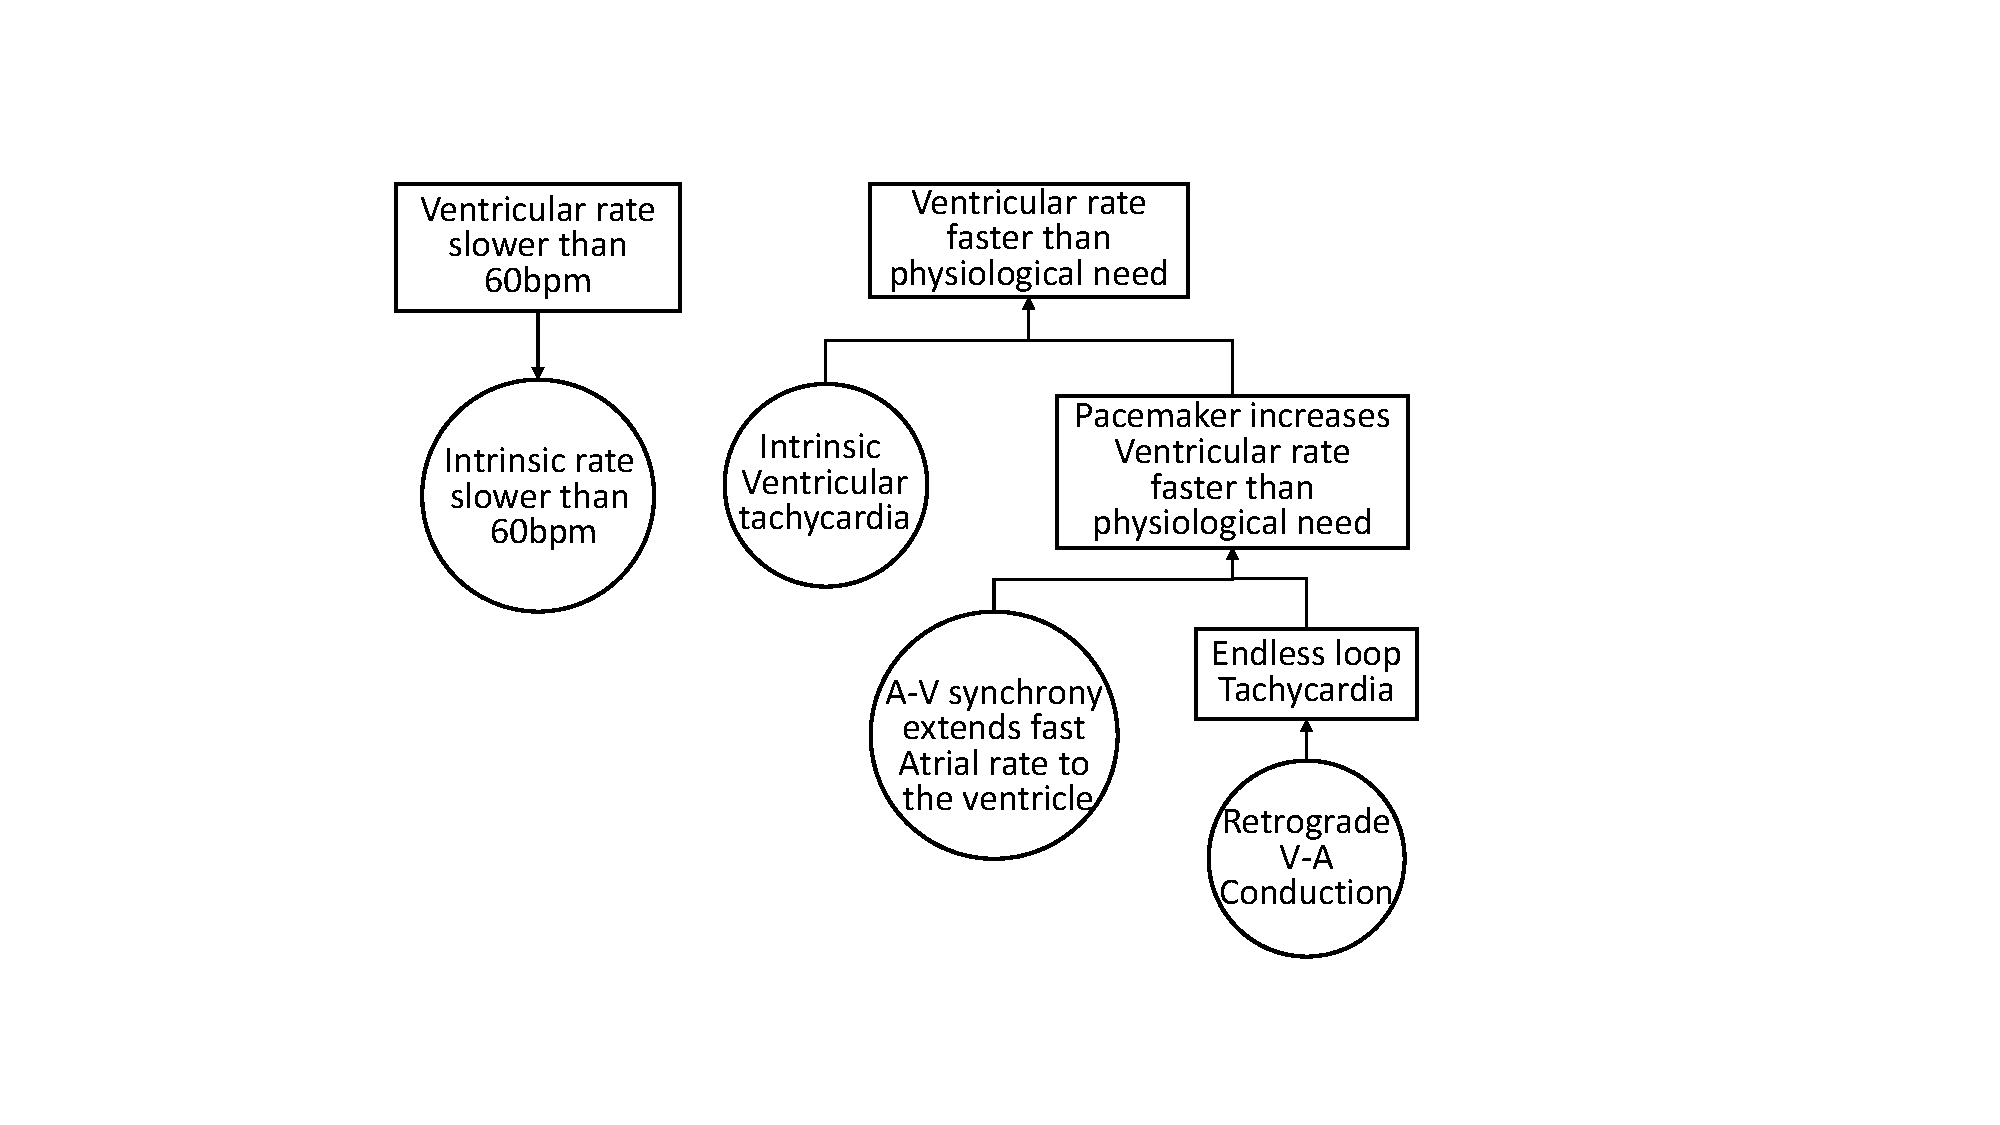
\includegraphics[width=0.8\textwidth]{figs/risk_requirements.pdf}
		\caption{\small Fault Tree Analysis (FTA) for two failures of a pacemaker}
		  %\vspace{-15pt}
		\label{fig:risk_req}
\end{figure}


\subsection{Endless-Loop Tachycardia}
\begin{figure*}
\centering
%		\vspace{-10pt}
		\subfigure [Virtual circuit formed by the pacemaker and the heart] {
				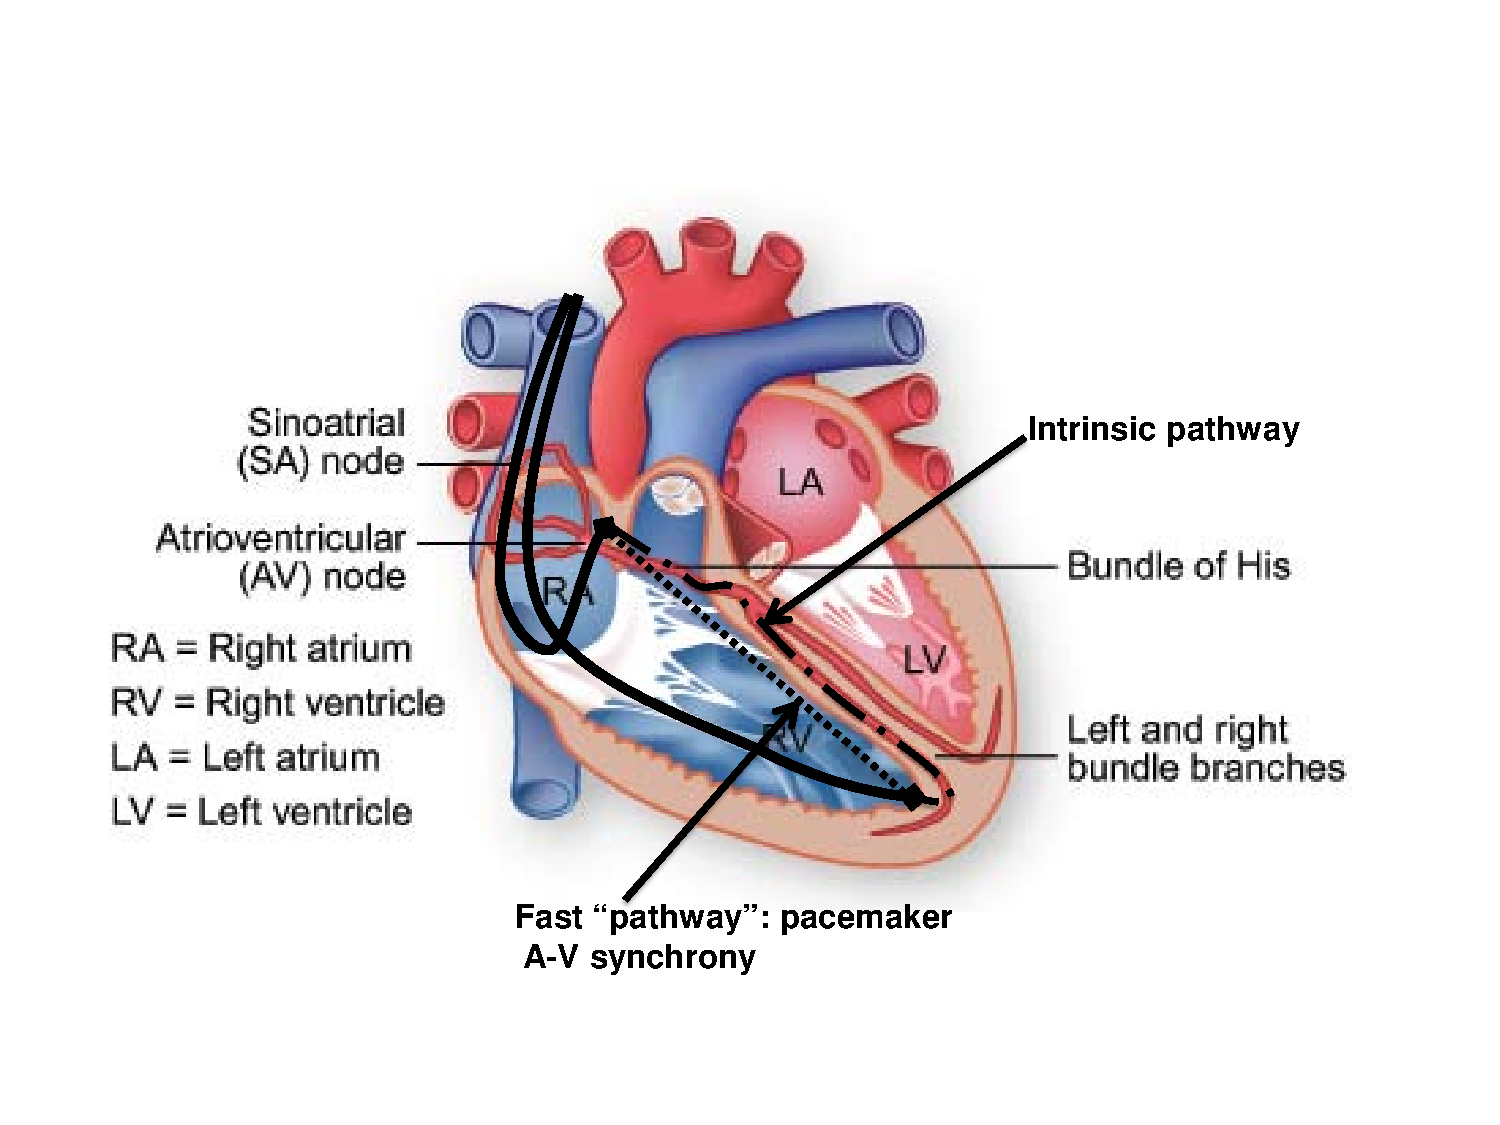
\includegraphics[width=0.45\textwidth]{figs/ELT_str.pdf}
				\label{fig:ELT_demo}
		} 
		\subfigure [Pacemaker trace for ELT initialized by a early ventricular signal]{	
			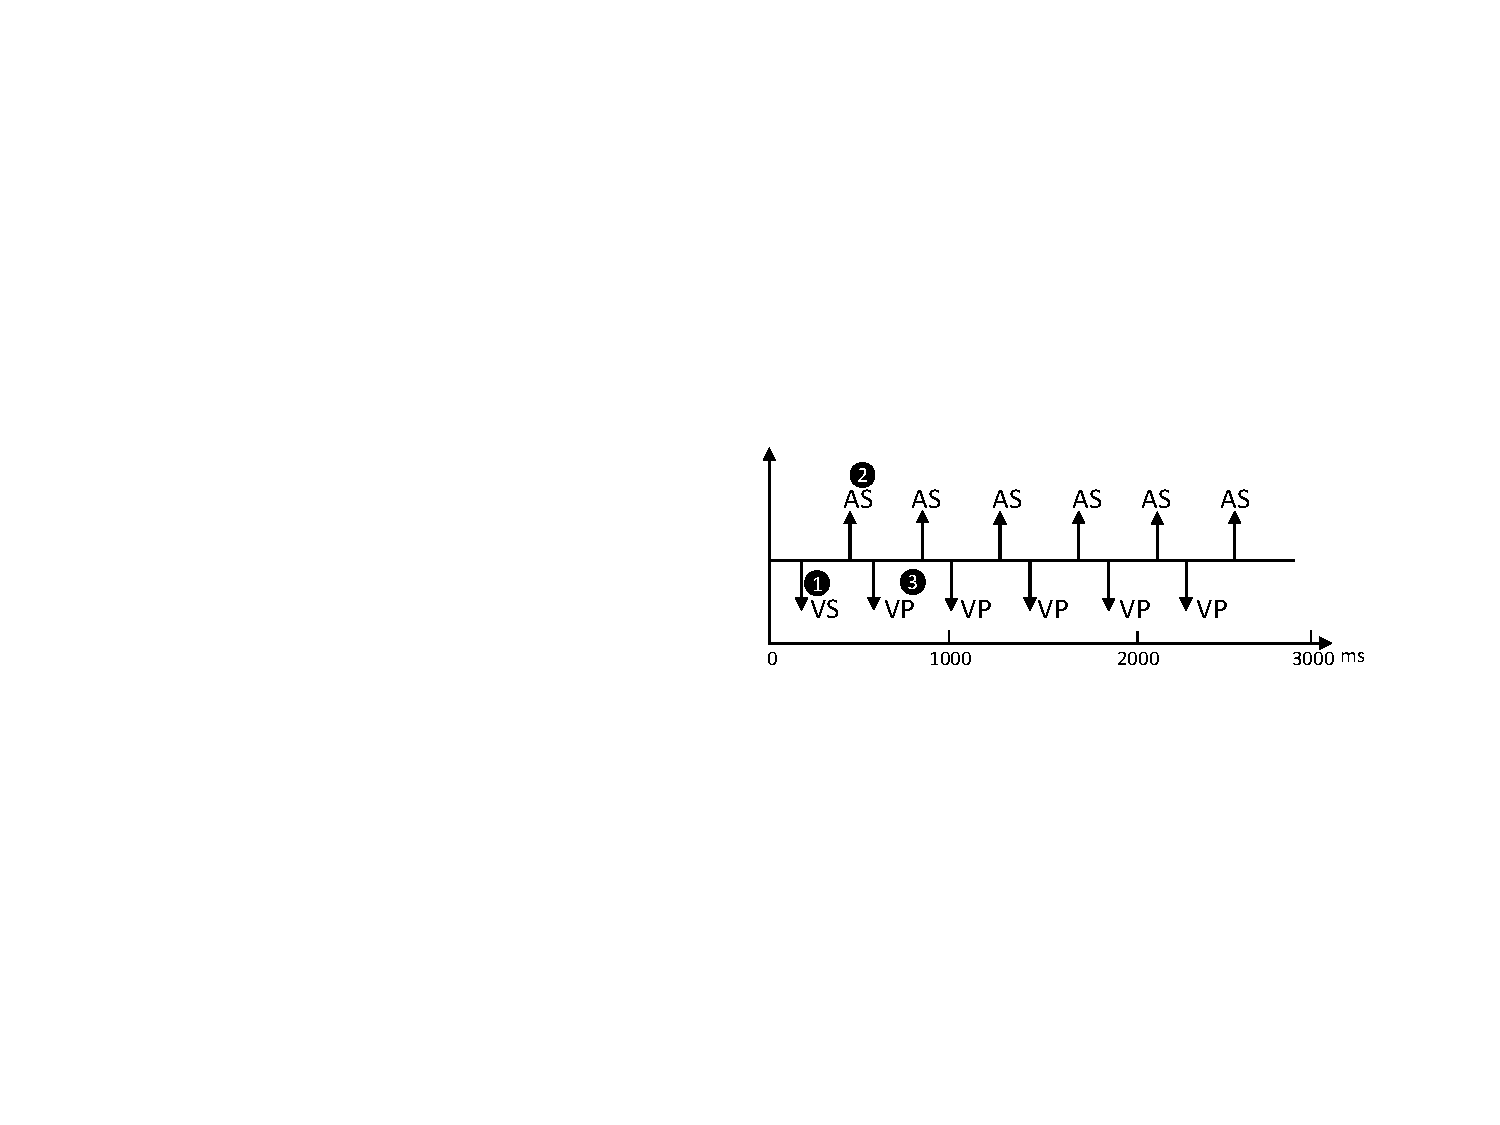
\includegraphics[width=0.45\textwidth]{figs/ELT.pdf}
			\label{fig:ELT}
		}
%		\vspace{-10pt}
	\caption{Endless Loop Tachycardia case study demonstrating the situation when the pacemaker drives the heart into an unsafe state \cite{vhm_iccps11}}
%\vspace{-15pt}
\end{figure*}

As introduced in the last section, a dual-chamber pacemaker paces the ventricle if no ventricular events are sensed after TAVI, which is equivalent to a virtual atria-to-ventricles conduction pathway. 
This forms a timing loop with the intrinsic (physiological) A-V conduction pathway (see \figref{ELT_demo}). 
A Premature Ventricular Contraction (PVC), i.e. an early extra beat in the ventricles, may trigger another ventricular event (VS) and initiate a V-A conduction through the intrinsic pathway (Marker 1 in \figref{ELT}). 
The pacemaker registers this signal as an Atrial Sense (AS) (Marker 2 in \figref{ELT}). 
A ventricular pace (VP) is delivered after TAVI, as if the signal conducts through the ``virtual" A-V pathway (Marker 3 in \figref{ELT}). 
The VP will trigger another V-A conduction and this VP-AS-VP-AS looping behavior will continue (see \figref{ELT}). 
The interval between atrial events is TAVI plus the V-A conduction delay, which is normally shorter than the delay between intrinsic heart beats, thus driving the ventricular rate as high as the Upper Rate Limit. 
During ELT, the heart rate is not only high, but also fixed without changing according to physiological need, which is an unsafe scenario.

\subsection{Atrial Tachycardia Response}

Supraventricular Tachycardia (SVT) is an arrhythmia with an abnormally fast atrial rate. %\figref{SVT} is a series of simulation results for closed-loop interaction between a heart model with SVT and the pacemaker model. The atrial and ventricular channels show electrogram inputs to the pacemaker and the pacemaker channel shows the corresponding events received and generated by the pacemaker software, \cite{vhm_embc11}.
Typically, in a heart without pacemaker, the AV node, which has a long refractory period, can filter most of the fast atrial activations during SVT, thus the ventricular rate remains relatively normal. \figref{SVT_none} demonstrates a pacemaker event trace during SVT, with a pacemaker in ODO mode, which just sensing in both channels. 
As there is no pacing in ODO mode, the heart is in open-loop with the pacemaker. In this particular case, every 3 atrial events (AS) correspond to 1 ventricular event (VS) during SVT. 
As an arrhythmia, SVT is still considered a safe heart condition since the ventricles operate under normal rate and still maintain adequate cardiac output. 

However, in the closed loop case with the DDD pacemaker, the AVI component of a dual chamber pacemaker is equivalent to a virtual pathway in parallel to the intrinsic conduction pathway between the atria and the ventricles. The pacemaker tries to maintain 1:1 A-V conduction and thus increases the ventricular rate inappropriately to match the atrial rate.  This is known as Pacemaker Mediated Tachycardia (PMT) as the heart would have been safe without the pacemaker and its virtual pathway. \figref{SVT_DDD} shows the pacemaker trace of the same SVT case with DDD pacemaker. Although half of the fast atrial events are filtered by the PVARP period ([AR]s), the DDD pacemaker still drives the closed-loop system into 2:1 A-V conduction with faster ventricular rate. Maintaining A-V delay is less important than maintaining an appropriate ventricular rate. The DDD pacemaker violates a higher priority requirement in order to satisfy a lower priority requirement, which is inappropriate.
\begin{figure*}[!t]
\centering
		\subfigure [\small]{			
		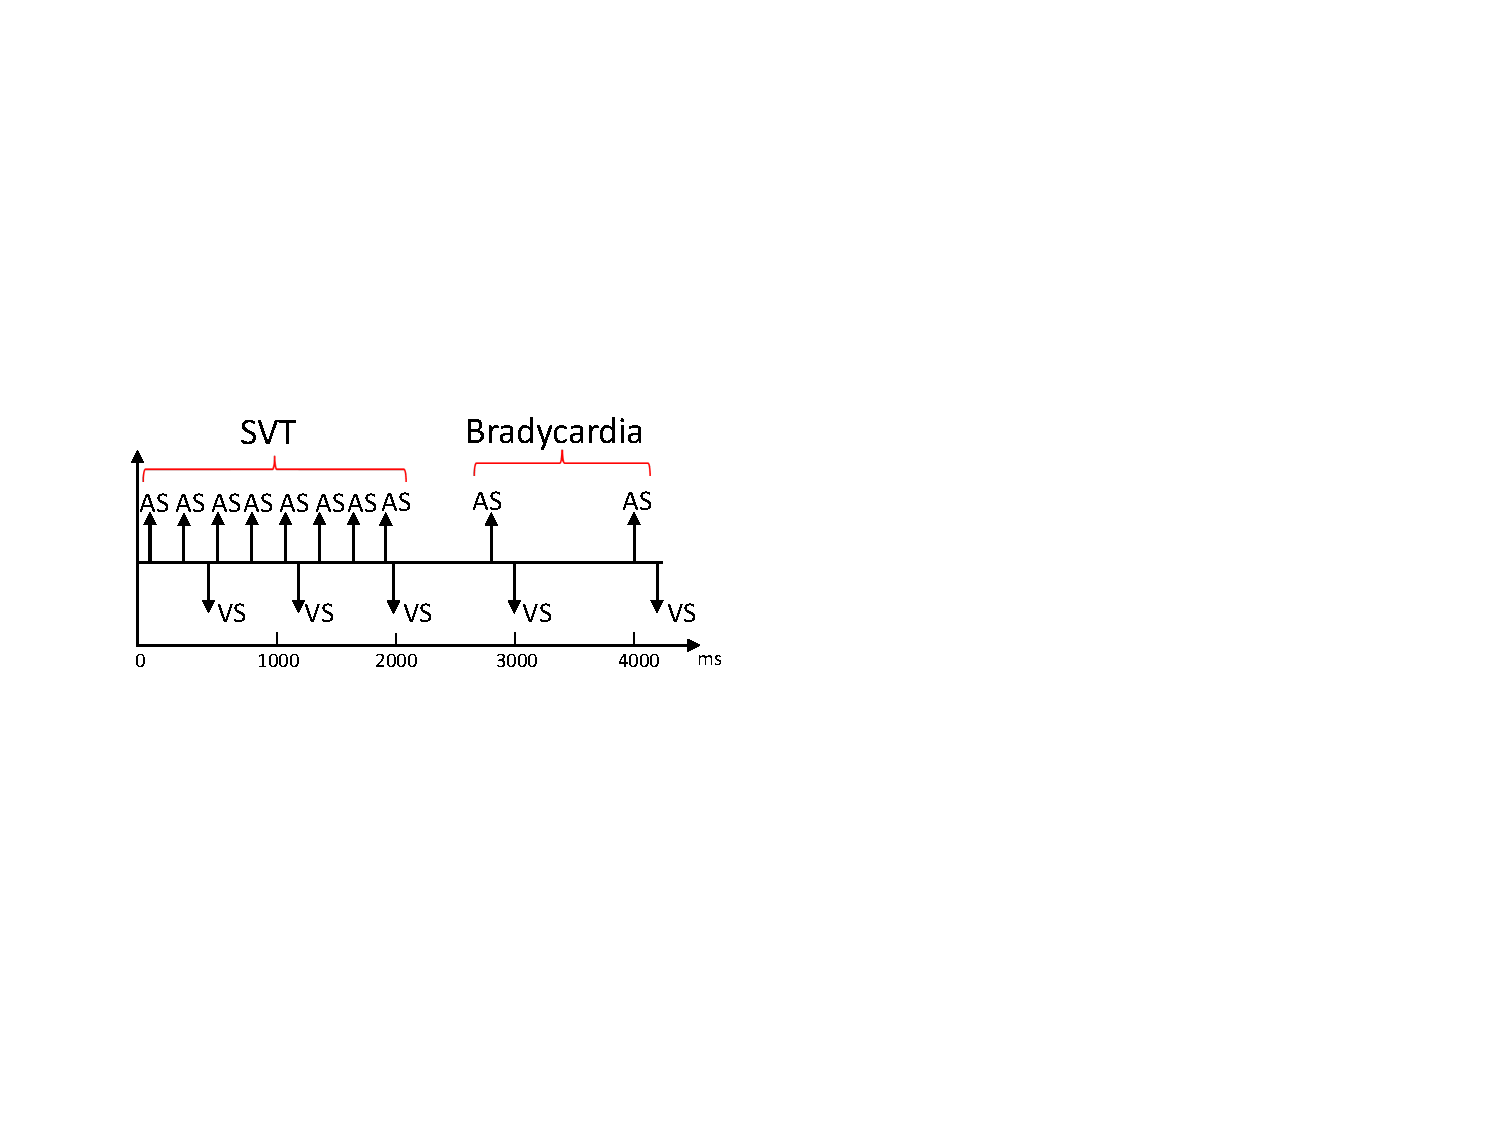
\includegraphics[width=0.45  \textwidth]{figs/SVT_none.pdf}
		\label{fig:SVT_none}
		} 
%	\hspace{.1in}%
		
		\subfigure [\small] 
		{
		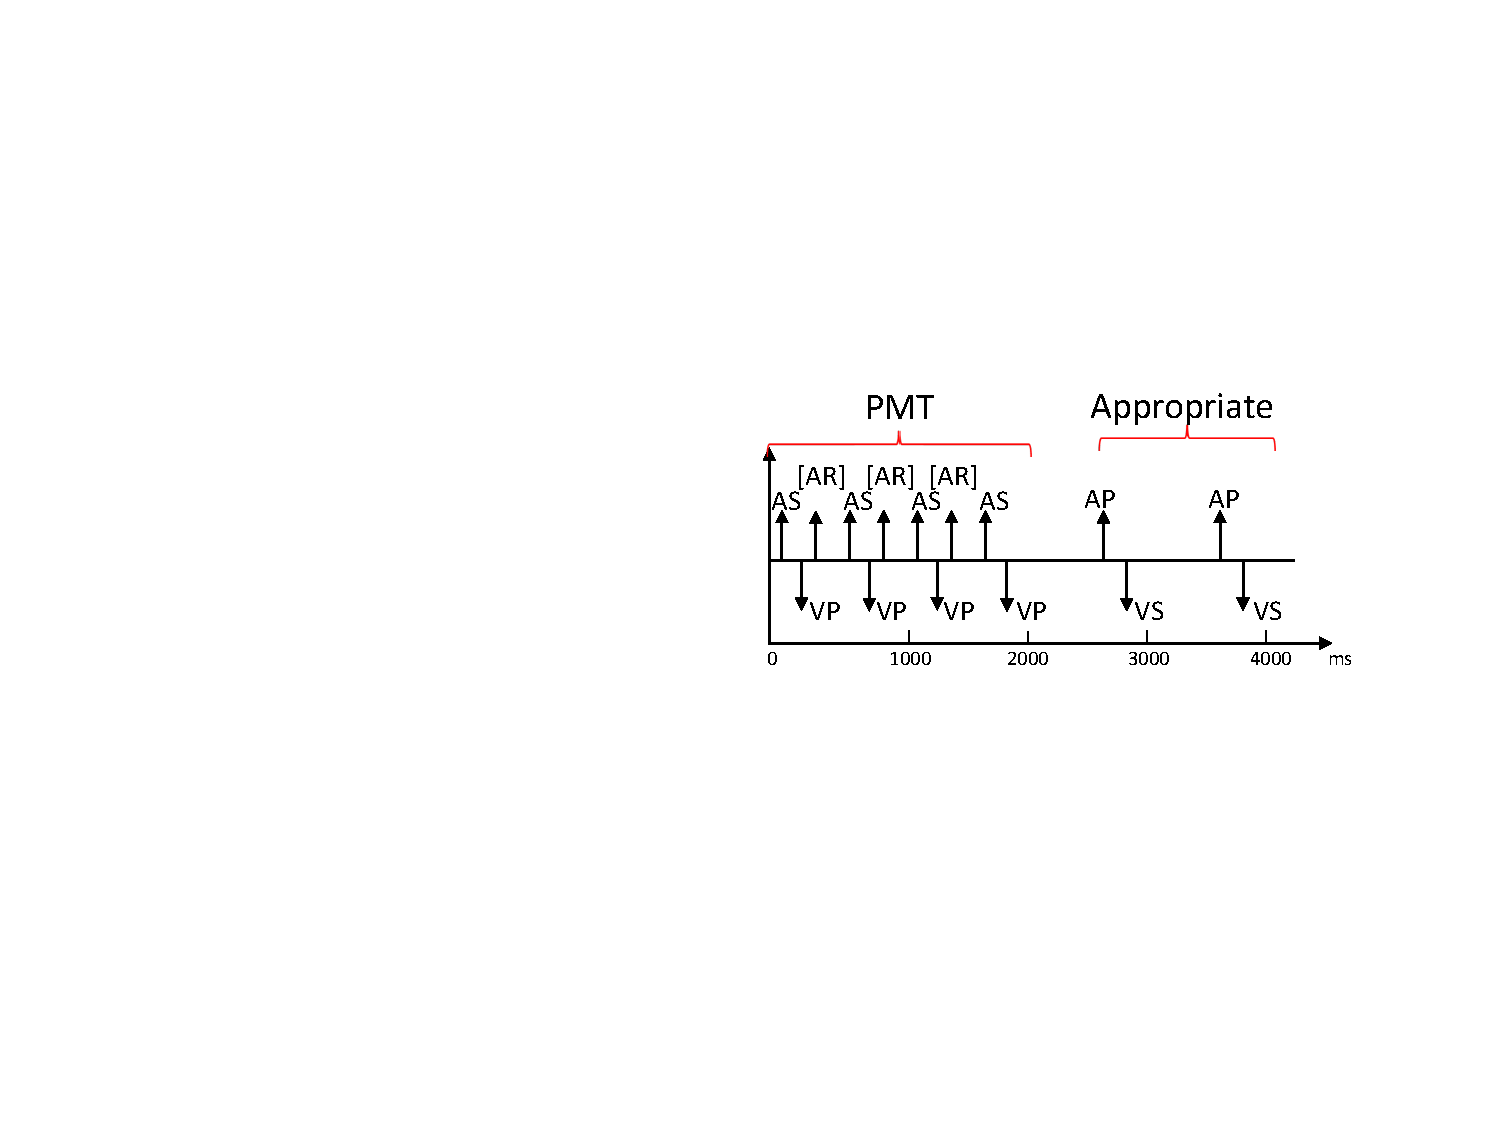
\includegraphics[width=0.45\textwidth]{figs/SVT_DDD.pdf}
		\label{fig:SVT_DDD}
		} 
\caption{\small Benign open loop case: SVT without a pacemaker or with a pacemaker in sense-only mode (ODO) (b) Dangerous closed-loop-case SVT with DDD pacemaker which tries to match the fast atrial rate with a corresponding (and dangerous) fast ventricular rate.}
\end{figure*} 

\section{Discussion}
Implantable cardiac devices such as implantable pacemakers are typical autonomous medical devices.
Despite their seemingly simple controller, the pacemakers also subject to the three challenges discussed in Chapter 1:
\begin{itemize}
	\item The physiology of the heart and its interaction with the rest of the body are complex.
\item The pacemakers have to safely operate within a large variety of physiological conditions.
\item A dual chamber pacemaker can only observe electrical activities from two local sites in the heart.
\end{itemize}
In the remaining dissertation, I will demonstrate the application of physiological models in various model-based techniques to provide safety and efficacy confidence to the pacemaker design.



\chapter{Theme 1: Modeling the Physiological Environment}

The safety and efficacy of autonomous medical devices have to be evaluated within their physiological environment. 
Models of human physiology can replace real patients and enable closed-loop evaluation earlier during device development.
%Models, especially models of the human physiology, which span a large spectrum of scale and complexity, should be designed in accordance with their respective applications.
In this chapter, a heart model structure is developed for closed-loop validation of implantable cardiac devices. This chapter aim to address the following questions:
\begin{itemize}
	\item How much detail does the physiological model need?
	\item How to validate the physiological model?
	\item What applications can the physiological models be used?
\end{itemize}

%Each application of the environment model has a different focus and has distinct modeling requirements which influence the model complexity and model identifiability.
%In an ideal physiological model for closed-loop evaluation of medical devices, details not affecting the interaction between the device and the physiology are abstracted away, while essential information required to differentiate different patient conditions are maintained. 
%As we will see, to validate the device operation across a range of physiological conditions and for a set of safety and efficacy properties, a family of models are needed which refine the closed-loop context to appropriately express the condition to be verified.

%\newpage
%\begin{itemize}
%\vspace{-5pt}
%\item How does the device interact with the physiological environment?
%\vspace{-5pt}
%\item What details must the physiological environment models capture?
%\vspace{-5pt}
%\item What are the different modeling philosophies when developing environment models for testing and for model checking?
%\end{itemize}



%\textbf{Model complexity:} How much detail should the physiological models have, in order to unambiguously describe a physiological behavior? In particular, if the model checker returns an execution trace as counter-example, how much details should the physiological model have so that the execution traces can be interpreted by domain experts? 	
%
%\textbf{Model Identifiability} is a metric for the feasibility of identifying model parameters from data. There are two methods for model construction: non-parametric modeling in which no prior knowledge is assumed and the model construction is purely data-driven; and parametric modeling in which domain knowledge of the physiological conditions is taken into account. For example, to model the electrophysiological activity of the heart, there is abundant literature describing the phenomena of individual arrhythmia, which makes parametric modeling of the environment favorable.

%%It affects the validity of the model which is a key element for closed-loop verification. Model identifiability is generally affected by the model complexity and the availability and quality of clinical data. 

%%The complexity requirements of an environment model is usually determined by 1) The complexity of the interactions between the environment model and the system model and 2) The complexity of the environment condition specified in the physiological requirements.

%In this chapter, a heart model structure is developed for closed-loop validation of the pacemaker design. 

\begin{figure}[!t]
\centering
		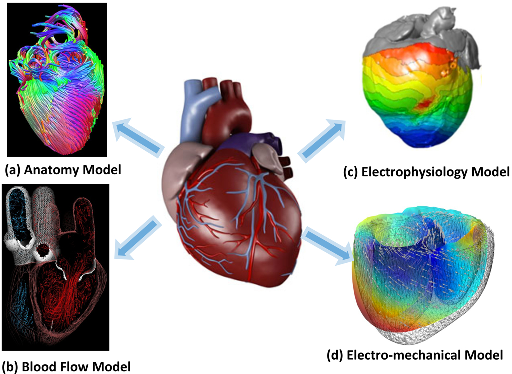
\includegraphics[width=0.9\textwidth]{figs/models.pdf}
		
%\vspace{-10pt}
\caption{\small Physiological models of the heart from different perspectives}
\label{fig:models}
%\vspace{-15pt}
\end{figure} 
\section{Related Work}
To study the mechanisms of heart diseases and their effects on cardiac output, different physiological models of the heart have been developed. 
\figref{models} illustrates several aspects that these models capture. 
With the development of the imaging techniques like MRI, detailed anatomical structures of the heart can be modeled and studied (\cite{geometric}). 
These models are fundamental in other modeling aspects as well, as the anatomy of the heart dictates the electrical and mechanical behaviors of the heart. 
\figref{models}.(a) shows models for heart muscle fiber orientations by \cite{fiber}. 
With anatomy models the electrical and/or mechanical properties of the heart can be studied. 
\figref{models}.(b) illustrate a model of blood flow within the ventricles (\cite{bloodflow}). 
Electrical properties of the heart at cellular level has been modeled (\cite{cellular}) and by combining these cellular models with the structural models, the electrical activities of the whole heart are studied, especially the mechanism of different arrhythmia (\cite{natalia},~\cite{Grosu_MHA},~\cite{Grosu_wave}). 
Intrinsic heart rate variability has been modeled to synthesize optimal control of pacemaker pacing. (\cite{Bogdan}) 
Abstraction of the electrical cellular model has also been attempted by \cite{Grosu_abstract} to reduce model complexity without sacrificing accuracy. 
The electrical properties and the mechanical properties of the heart are closely coupled. 
Models combining both of these aspects are also developed to study the effects of different arrhythmia on cardiac outputs (\cite{natalia},~\cite{eletro_mechanical}).

\section{EP Heart Model Structure for Closed-loop Validation of Implant-able Cardiac Devices}
Models should be designed in accordance with their respective applications. 
The aforementioned models of the heart are designed for understanding the mechanisms of different heart diseases. 
For closed-loop evaluation of autonomous medical devices, physiological modeling should have the following considerations:\\
\textbf{C1. Interfacing with the device: }The model should be able to generate physiological signals that the device sense from the real physiological entities. 
The model should also be able to take device output as input and change its states accordingly. 
Model complexity should also be adjusted according to the device interface to hide unnecessary details.\\
\textbf{C2. Differentiate different physiological conditions: }To evaluate the safety and effectiveness of the device, the device has to be evaluated under certain physiological conditions specified by the requirements. 
For example, the pacemaker is supposed to maintain proper heart rate during Bradycardia. 
The model should be expressive enough to be able to differentiate the physiological condition (Bradycardia in the example) from other conditions. 
Failing to do so may result in false-positives or false-negatives in the evaluation result. \\
\textbf{C3. Physiological/logical interpretation of model states: } In closed-loop evaluation we are checking the device safety and effectiveness against the physiological requirements. 
However, due to the limited interface (e.g. two leads for a dual chamber pacemaker) it is always difficult to determine only from an execution trace that the therapy is safe and effective. 
Therefore, being able to provide physiological meanings to the states of the model also allows us to interpret the closed-loop execution more accurately, thus reducing the number of physiologically invalid executions during the evaluation. 
To satisfy these requirements, the model structure of these physiological models should base on physiological or clinical first principles so that states and state transitions of the closed-loop executions can be explained with physiological language. \\%One advantage of closed-loop evaluation over open-loop evaluation is the capability to provide physiological/logical interpretation of an execution trace. With this advantage we are able to identify and reduce the number of physiological-impossible executions by examining the state of the model, so that the evaluation can focus on physiological-possible executions. This requires the model first-principle\\
\textbf{C4. Available patient data: } In closed-loop evaluation, physiological models are developed to represent certain physiological condition across a population of patients or even particular patients. 
The model parameters must be identified so that the behaviors of the models match the behaviors of the patients (groups).  Due to the limited sensing capability of closed-loop medical devices, the obtained data is sparse: i.e. we can not put a sensor on every tissue region of the heart. 
Therefore the complexity of the model should be in accordance with the available data to avoid \emph{over-fitting}, which occurs when a model has too many parameters relative to the number of observations, and this can introduce errors during prediction. 

The electrophysiological models mentioned in the last section (\cite{natalia,Grosu_MHA}) satisfy C1-C3. 
However, the parameter space of these models are too large (10+ parameters for each cellular model multiplied by $10^5$ of elements) which not only increase simulation complexity, but also impossible to identify due to lack of data. 
As introduced in Section \ref{EP}, the pacemaker has only two leads at fixed locations and only use timing between local activation events for diagnosis. 
These models with high spatial fidelity possess details that can be abstracted without sacrificing the model accuracy.

Electrophysiology testing (EP testing) has been an active clinical field to diagnose and treat arrhythmia with minimal-invasive procedures. 
During an EP testing procedure, the physicians diagnose heart conditions by examining the patterns and intervals of local electrical activations (temporal) measured from electrodes placed into different locations of the heart (spatial). 
EP testing is the perfect level of abstraction for closed-loop evaluation of implantable cardiac devices because: 1) it is the basis of implantable cardiac devices (C1), 2) physicians can use EP testing to diagnose most arrhythmia thus distinguish them (C2,C3), and 3) there are abundant patient data available (C4). 

In the remaining chapter we will introduce the heart model structure based on EP testing, and model adaptation for two different applications of closed-loop evaluation of implantable cardiac devices.
%\section{Heart Models for Pacemaker Interaction}
%The heart generates electrical impulses to maintain the heart rate appropriate for the physiological needs. These impulses conduct through the heart, triggering coordinated muscle contractions which pumps blood to the rest of the body. The underlying pattern and timing of these impulses determines the heart's rhythm and is key to proper heart function. Derangements in this rhythm are referred to as \emph{arrhythmia}, which 



%\subsection{Electrical conduction system of the heart}
%Heart tissue with different timing parameters form the electrical conduction system to ensure coordinated contraction of the heart. First, specialized tissue at the Sinoatrial (SA) node periodically and spontaneously self-depolarizes. This is controlled by the nervous system and the SA node is the primary and natural pacemaker of the heart. The activation signal then travels through both atria, causing contraction and pushes blood into the ventricles. Then the activation is delayed at the Atrioventricular (AV) node which allows the ventricles to fill fully. The fast-conducting His-Purkinje system then spreads the activation signal within both the ventricles. The simultaneous contraction of the ventricle muscles will push the blood out of the heart.
%\begin{figure*}[!t]
%\centering
		%\subfigure [\small]{			
		%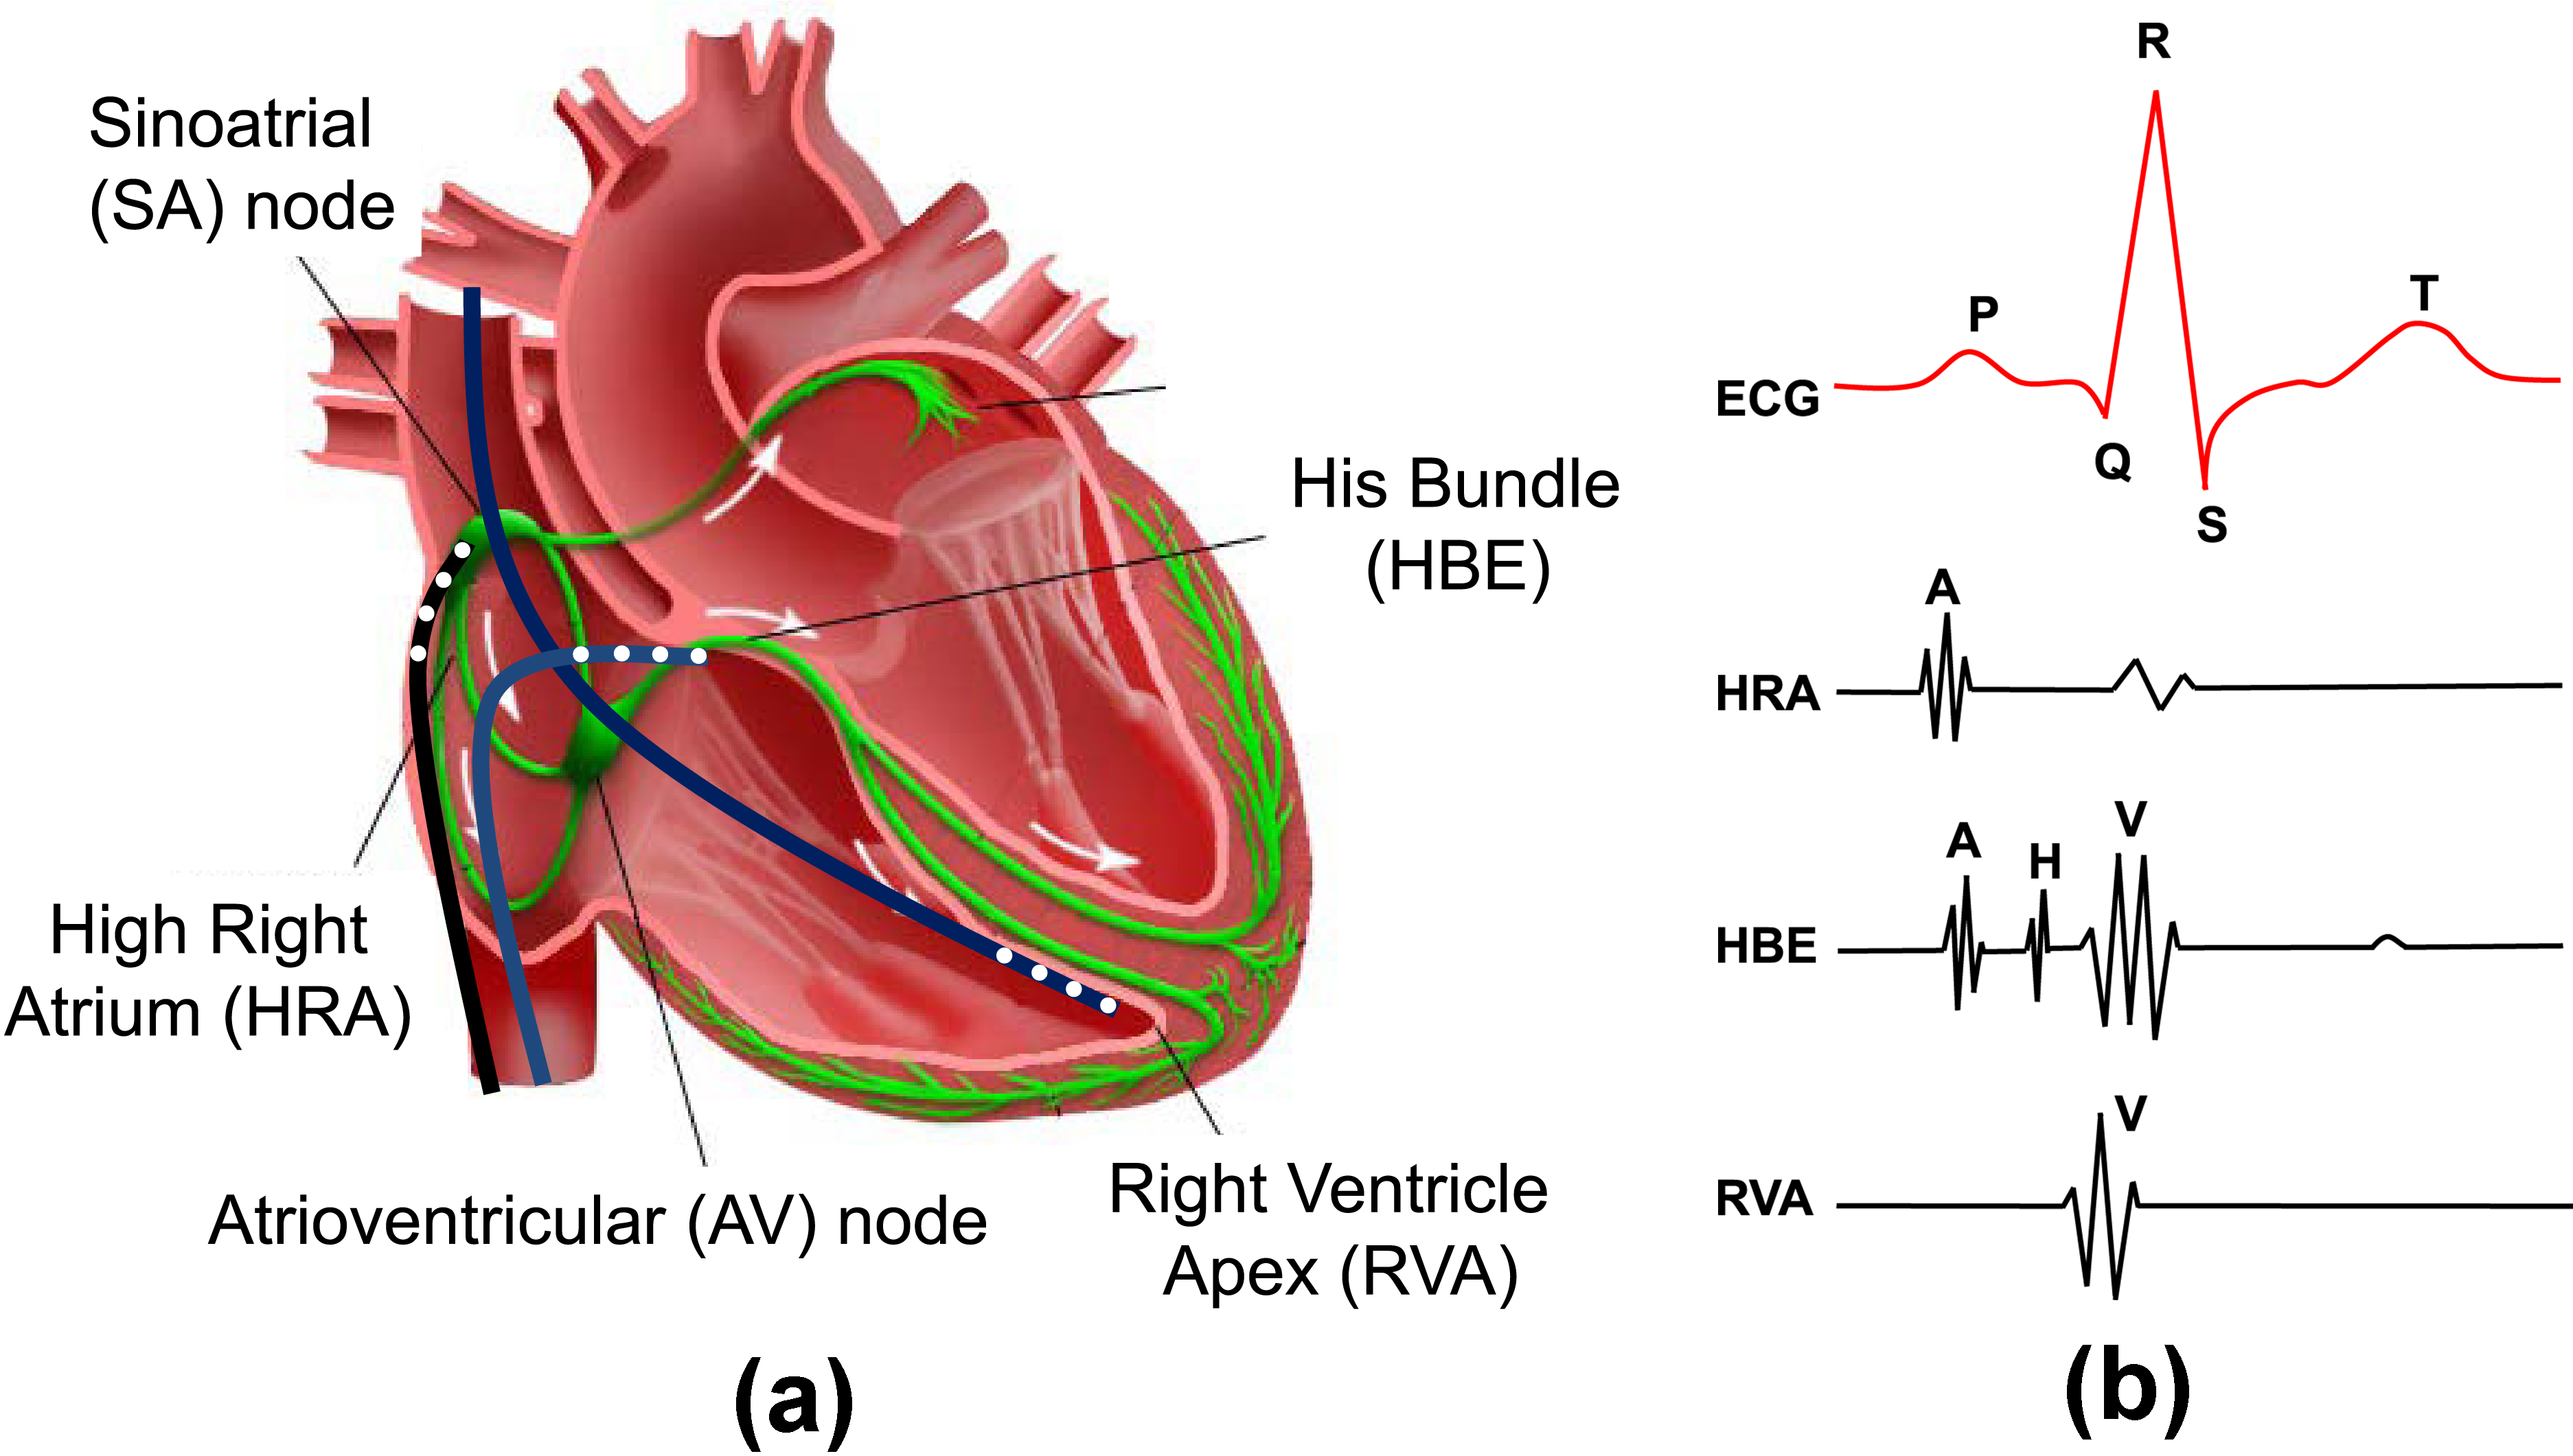
\includegraphics[width=0.3  \textwidth]{figs/probes.png}
		%\label{fig:probes}
		%} 
%
		%\subfigure [\small] 
		%{
		%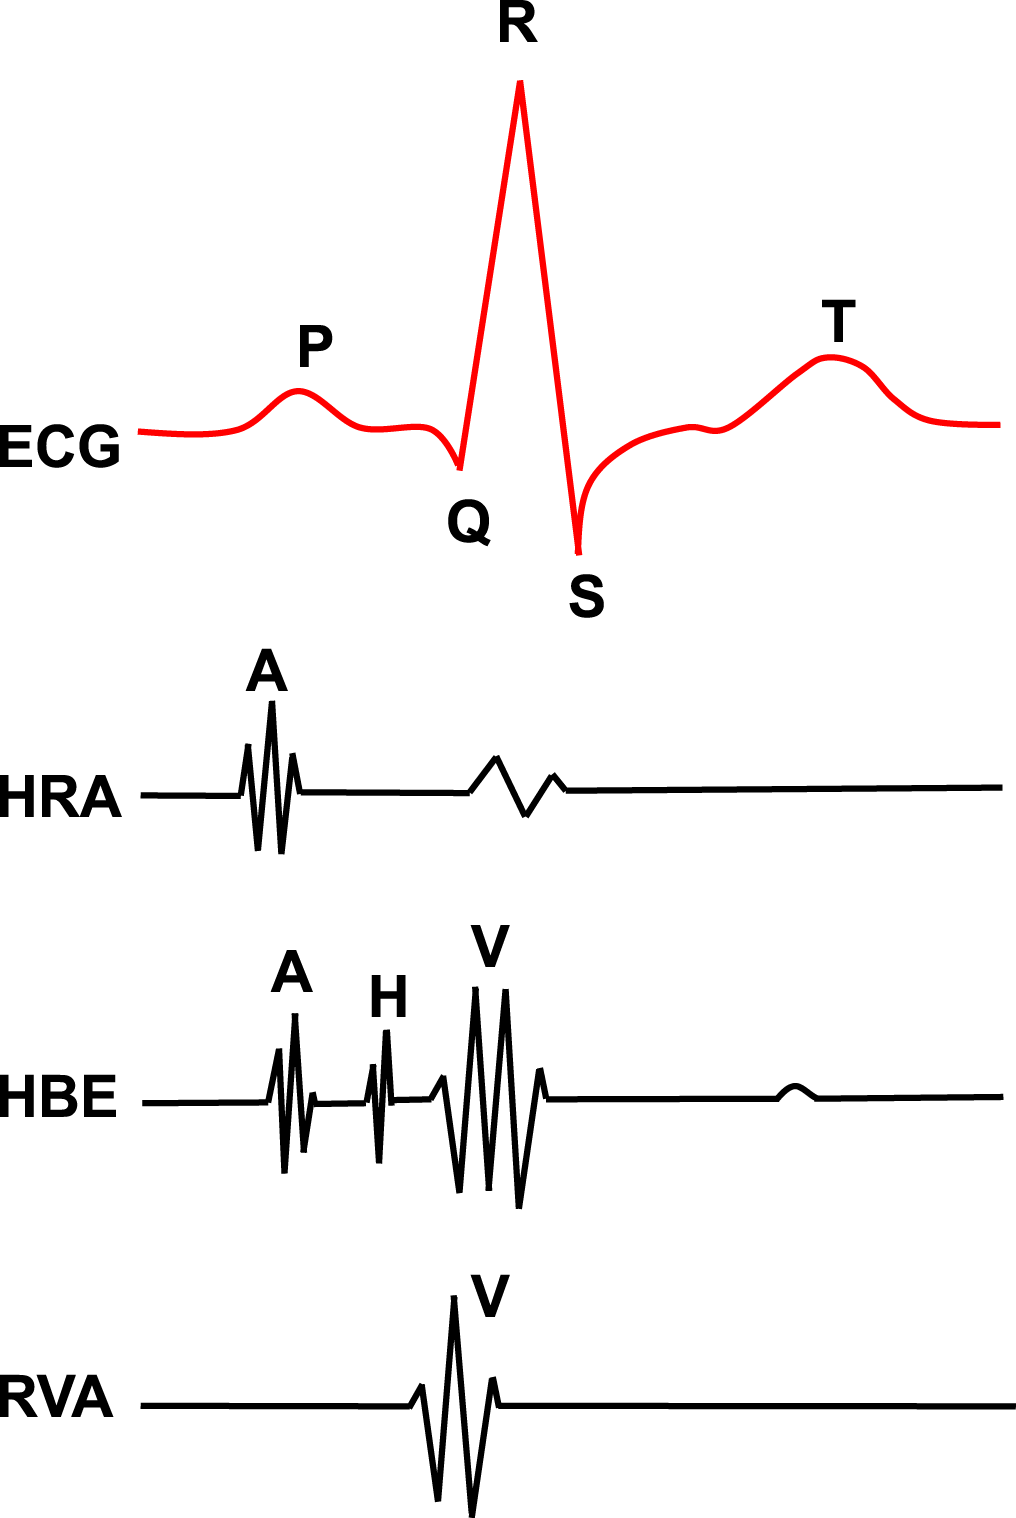
\includegraphics[width=0.2\textwidth]{figs/egm.png}
		%\label{fig:egm}
		%} 
%%\vspace{-10pt}
%\caption{\small (a) Node automaton. Dotted transition is only valid for pacemaker tissue like SA node; (b) Path automaton; (c) Model of the electrical conduction system of the heart using a network of node \& path automata~\cite{vhm_ecrts10}.}
%%\vspace{-15pt}
%\end{figure*} 

%\section{Electrophysiological Testing}
%\Hao{A figure for heart and pacemaker}

%\chapter{Modeling the Physiological Environment}
%\begin{itemize}
	%\item How to encode domain knowledge of the physiological environment into models?
    %\item What are the applications that the models will be used?
    %\item What are the differences in terms of environment models between model checking and simulation?
    %\item How to balance complexity and expressiveness of the model?
%\end{itemize}

%In the following sections, we demonstrate how to construct heart models for closed-loop verification of implantable pacemaker. Note that for two different applications the models are constructed differently as we address their respective requirements for environment models. 


%\begin{itemize}
	%\item Why the models at this level have to be deterministic? Where can they be used?
    %\item How electrophysiology reflects the functions of the heart?
    %\item How to encode these knowledge into models?
    %\item Why VHM has the right level of details for pacemaker verification?
    %\item How VHM interacts with pacemaker?
    %
%\end{itemize}
%During closed-loop testing, the devices interact with the environment (or its models) under different environmental conditions. The closed-loop executions are monitored and violations of safety and efficacy requirements are reported. In model-based closed-loop testing, the environment models are expected to mimic the behaviors of actual environment and its interaction with the device. Thus, the environment models are in general deterministic so that the execution traces are reproducible and are able to mimic different arrhythmia. Complex dynamics during state transitions also need to be captured to validate violations within longer executions traces. 


\begin{figure}[!t]
\center
%\vspace{-10pt}
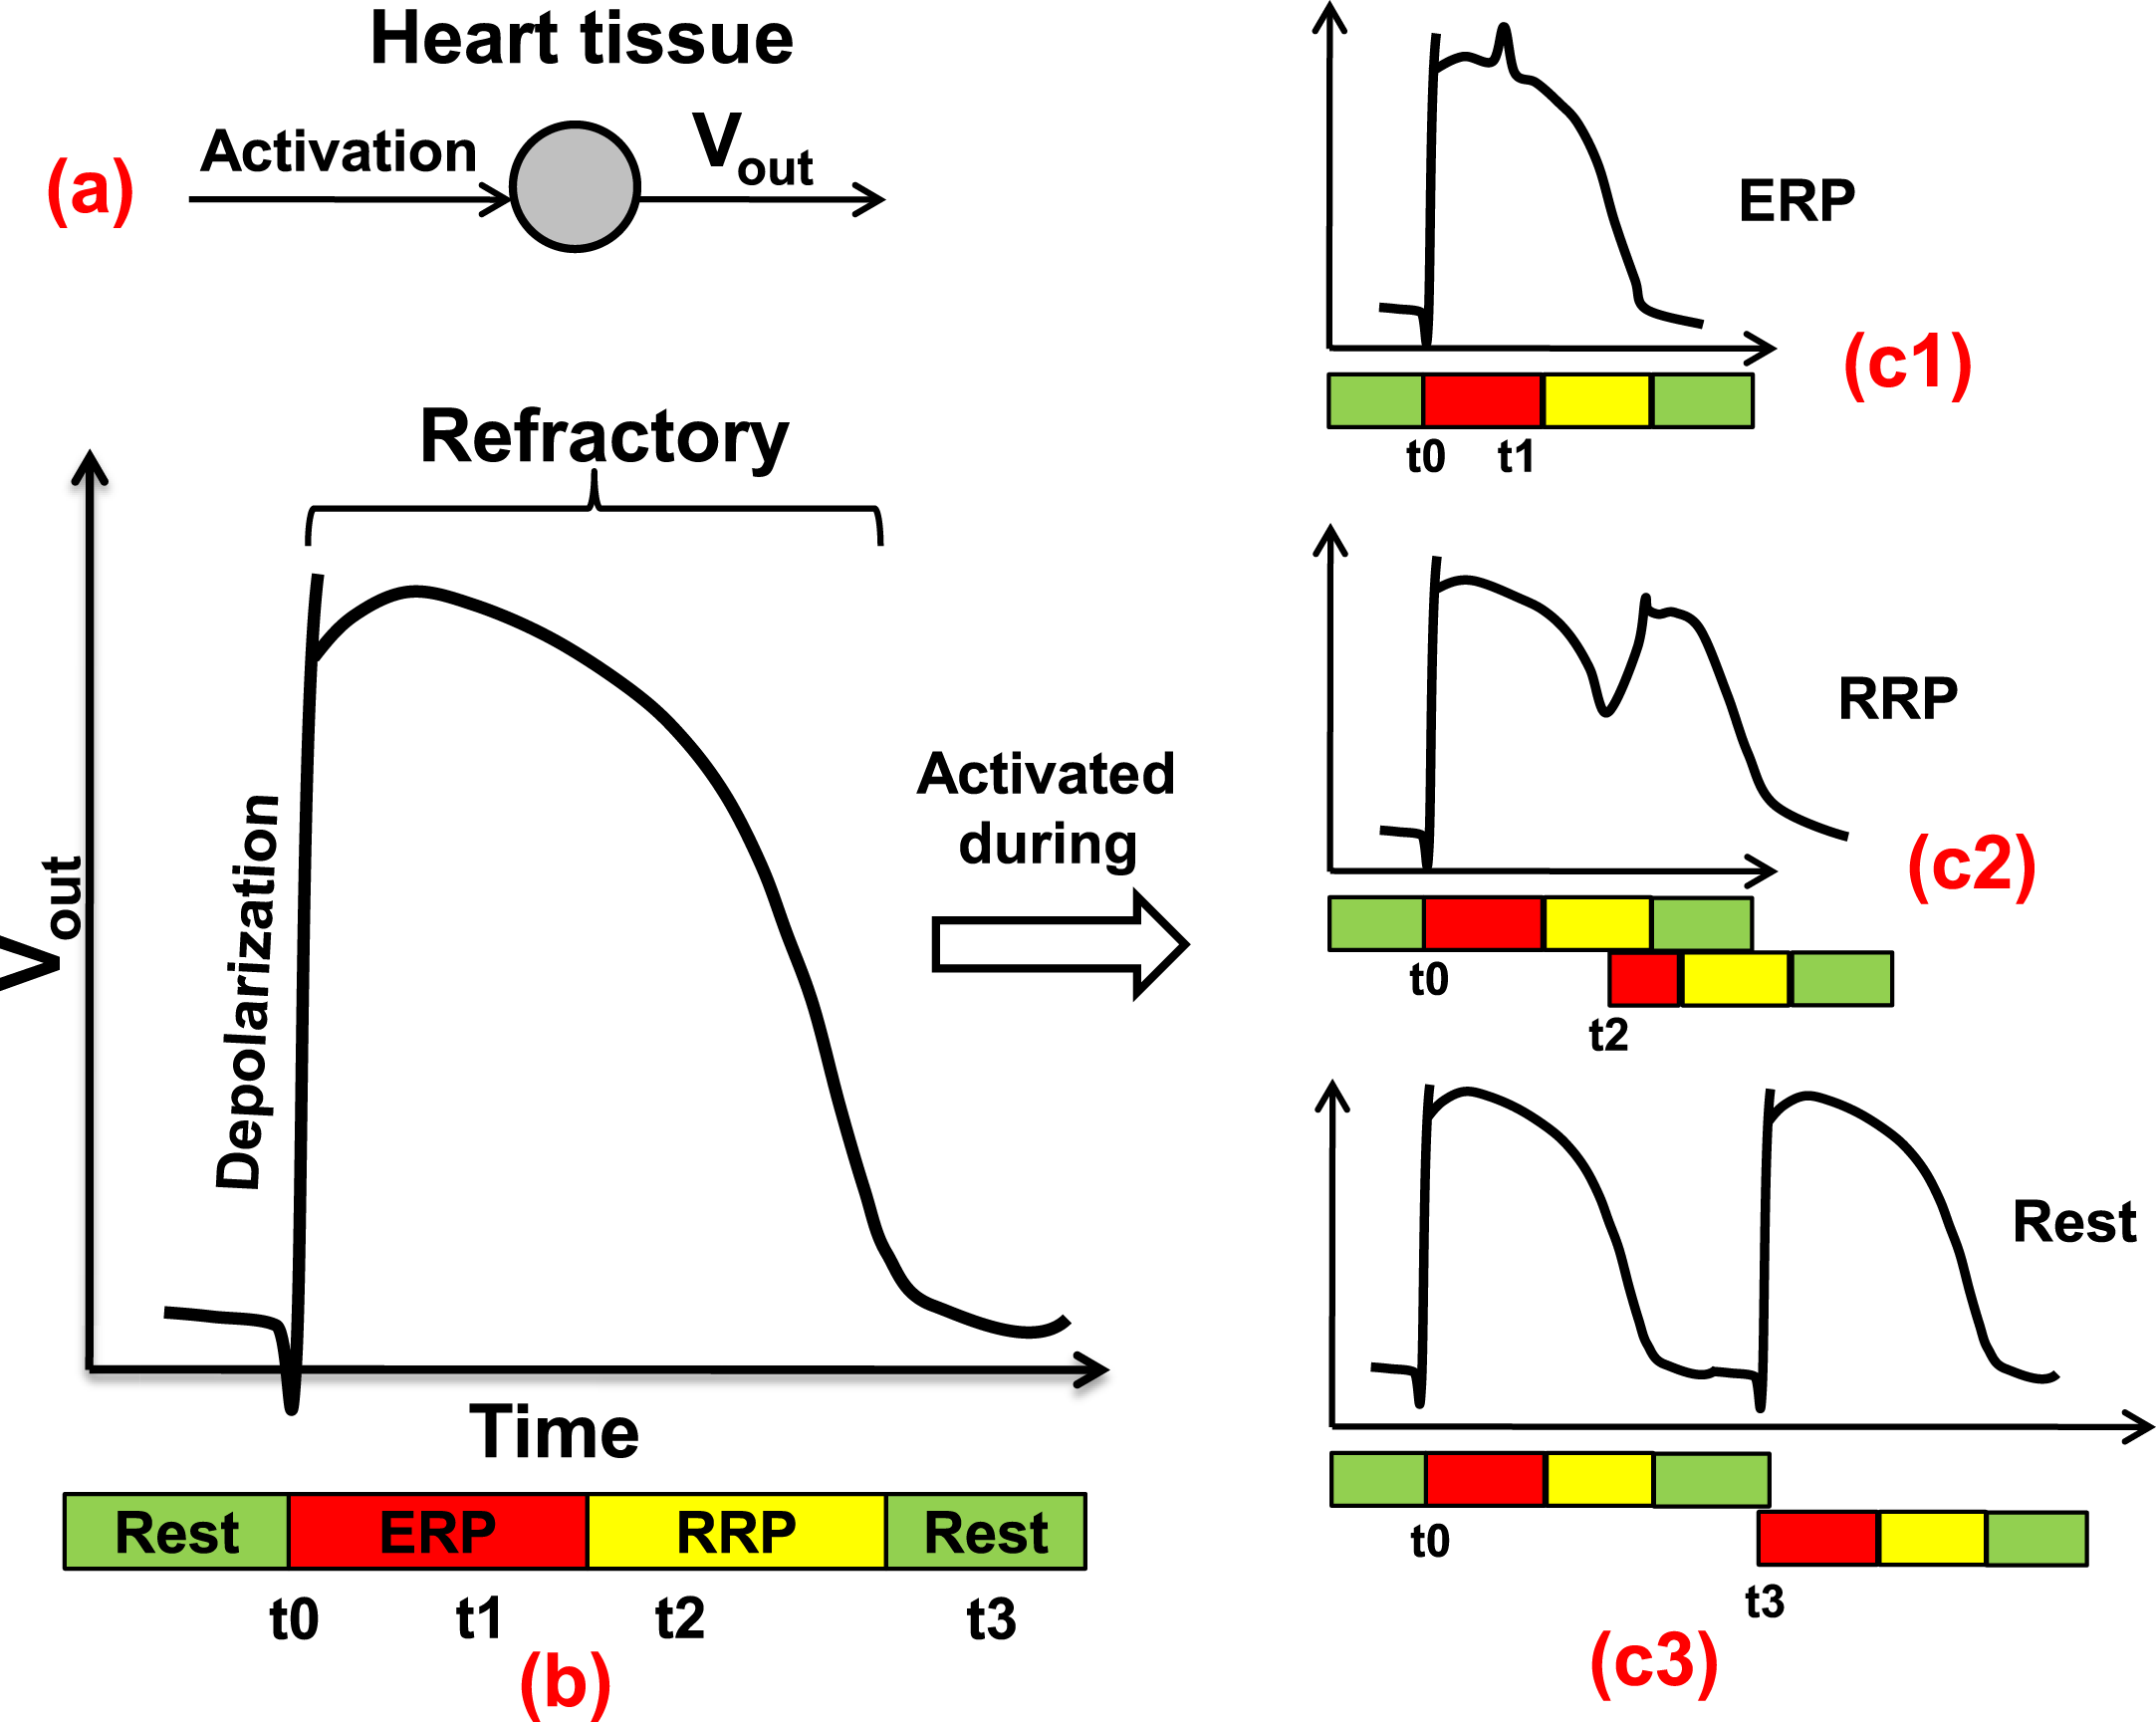
\includegraphics[width=0.7\textwidth]{figs/refractory.png}
%\vspace{-10pt}
\caption{(a) The generation of Action potential; (b) Action potential; (c1) The second activation arrived during ERP; (c2) Arrived during RRP; (c3) Arrived after refractory.}
\label{fig:refractory}
%\vspace{-10pt}
\end{figure} 
\subsection{Timing Behaviors of Cellular Electrophysiology}
The contraction of heart muscles is triggered by external voltage applied to the tissue. After the activation, a transmembrane voltage change over time can be sensed due to ion channel activities, which is referred to as an Action Potential (\figref{refractory}(a)). The upstroke of the action potential is called depolarization, during which the muscle will contract. The voltage change caused by the depolarization will depolarize the tissue nearby, which causes an activation wave across the heart. After the depolarization there is a refractory period during which the tissue recovers to the pre-excitation state and the voltage drops down to the resting potential. The refractory period can be divided into \emph{Effective Refractory Period (ERP)} and \emph{Relative Refractory Period (RRP)} (\figref{refractory}(b)). During ERP, the tissue cannot be depolarized due to the lack of charge. As a result, the activation wave will be "blocked" at the tissue during ERP (\figref{refractory}(c1)). During RRP, the tissue is partially recovered and the tissue can be depolarized. However, the new action potential generated by the depolarization will have different morphology (e.g. attenuated in magnitude and duration), thus affecting the refractory periods of the tissue and conduction delay of the activation wave (\figref{refractory}(c2)). \figref{refractory}(c1)-(c3) show the action potential shape change and corresponding timing change in refractory periods when the tissue is activated at time stamp $t1$, $t2$, $t3$ after the initial activation $t0$. 

\subsection{Heart Model Components}
We introduce the model components that can be used to configure heart models corresponding to different heart conditions. As discussed earlier, the action potential of a heart tissue has 3 timing periods during which the tissue responds to external electrical stimuli differently. We use an extended timed-automata formulation (\cite{timed_automata}) to model the timing behaviors of a heart tissue during each cycle. 

\textbf{Node Automata:} We refer to the tissue model as \emph{node automaton} and \figref{automata}.(a) shows the structure of a node automaton $i$. 3 states correspond to the timing periods of the action potential. From \textsf{Rest} state, the node can either self-activate or get activated by external stimuli (Act\_node) and go to \textsf{ERP} state. During \textsf{ERP} state the node does not respond to external stimuli (blocked). During \textsf{RRP} state, the node can still be activated and go to \textsf{ERP} state, however the ERP period and the conduction delay of the tissue are affected by the "earliness" of the activation arrived during the RRP period, which is tracked by a shared variable $C(i)$. The new ERP period is determined by a function over clock value $g(f(t))$ which mimics the beat-to-beat dynamics described in \cite{josephson}. The function $g$ and $f$ are given by:
\begin{equation} \label{factor}
						f(t) = 1-t/Trrp
						\end{equation}
and
%  The AV node has a different profile than the other tissue. The ERP period increases rather than decreases when activated during its RRP (~\cite{josephson}).
\begin{equation} \label{earliness_noAV}
						g(x) = \left\{
						\begin{array}{lr}
						
						T_{min}+(1-(1-x)^3)\cdot (T_{max}-T_{min}), i=AV\\
						T_{min}+(1-x^3)\cdot (T_{max}-T_{min}),i\neq AV
			
						
						\end{array}
						\right.
						\end{equation}  
where $T_{min}$ and $T_{max}$ are the minimum and maximum value for \emph{Terp} of the tissue.
\begin{figure}[!t]
%\centering
		%\subfigure [\small]{			
		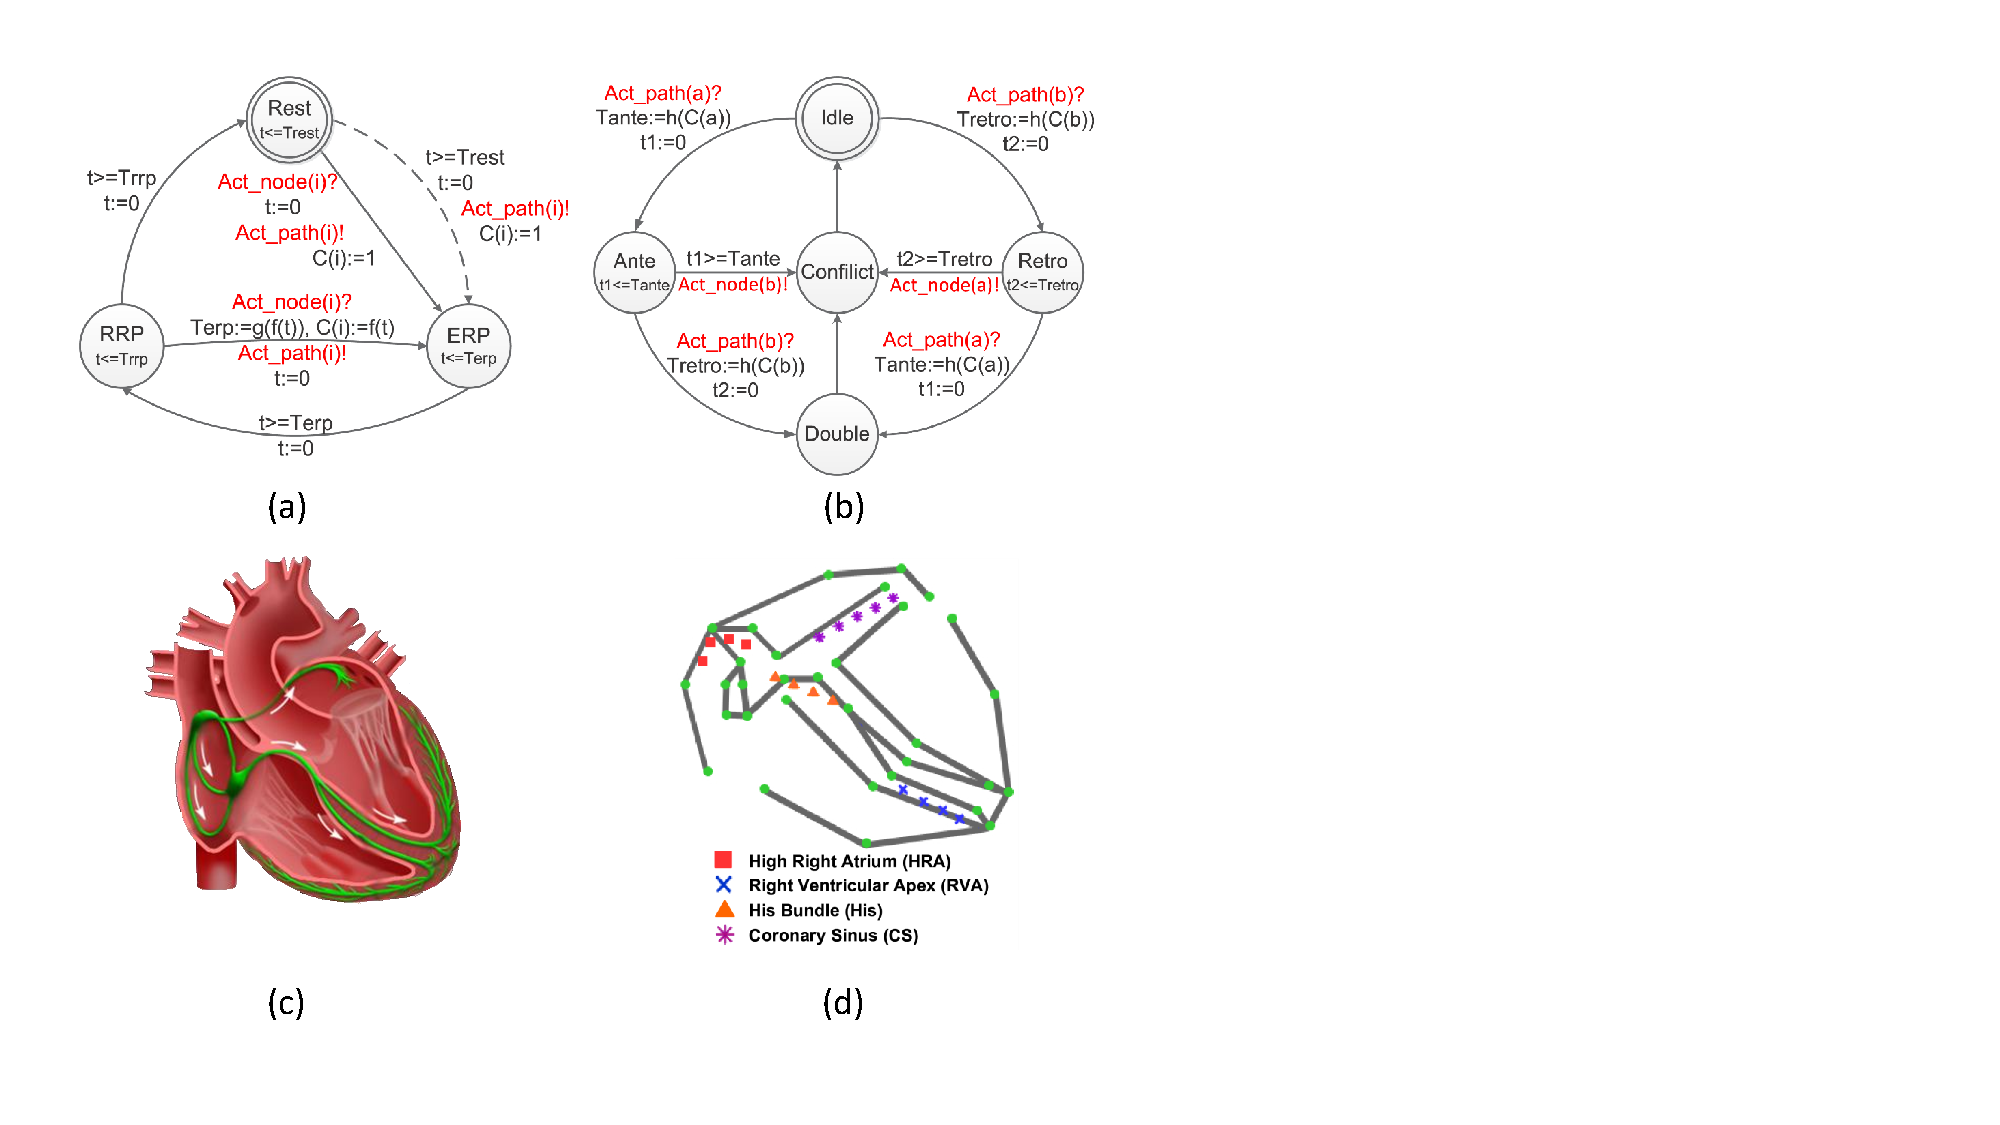
\includegraphics[width=\textwidth]{figs/automata.pdf}
		%\label{fig:node_automata}
		%} 
%%	\hspace{.1in}%
		%\subfigure [\small] 
		%{
		%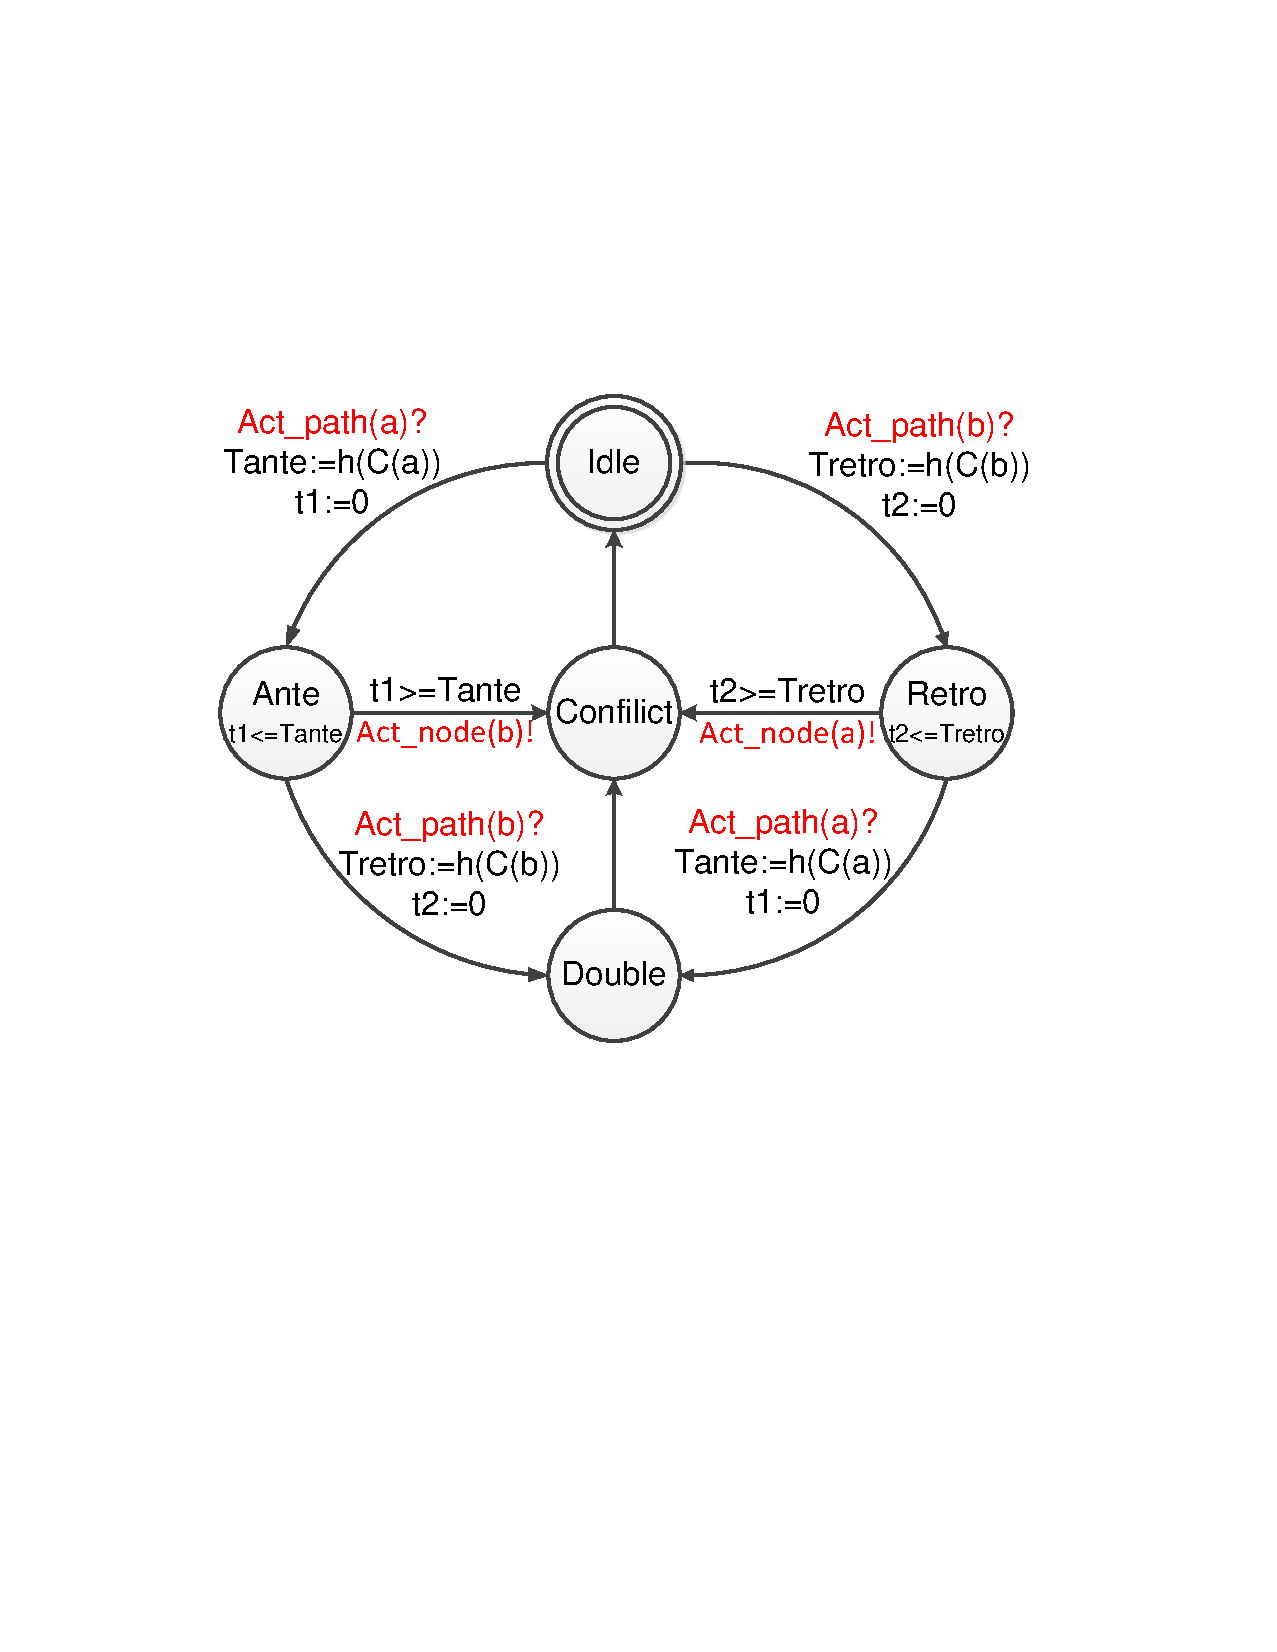
\includegraphics[width=0.32\textwidth]{figs/path.pdf}
		%\label{fig:path_automata}
		%} 
		%\subfigure [\small] 
		%{
		%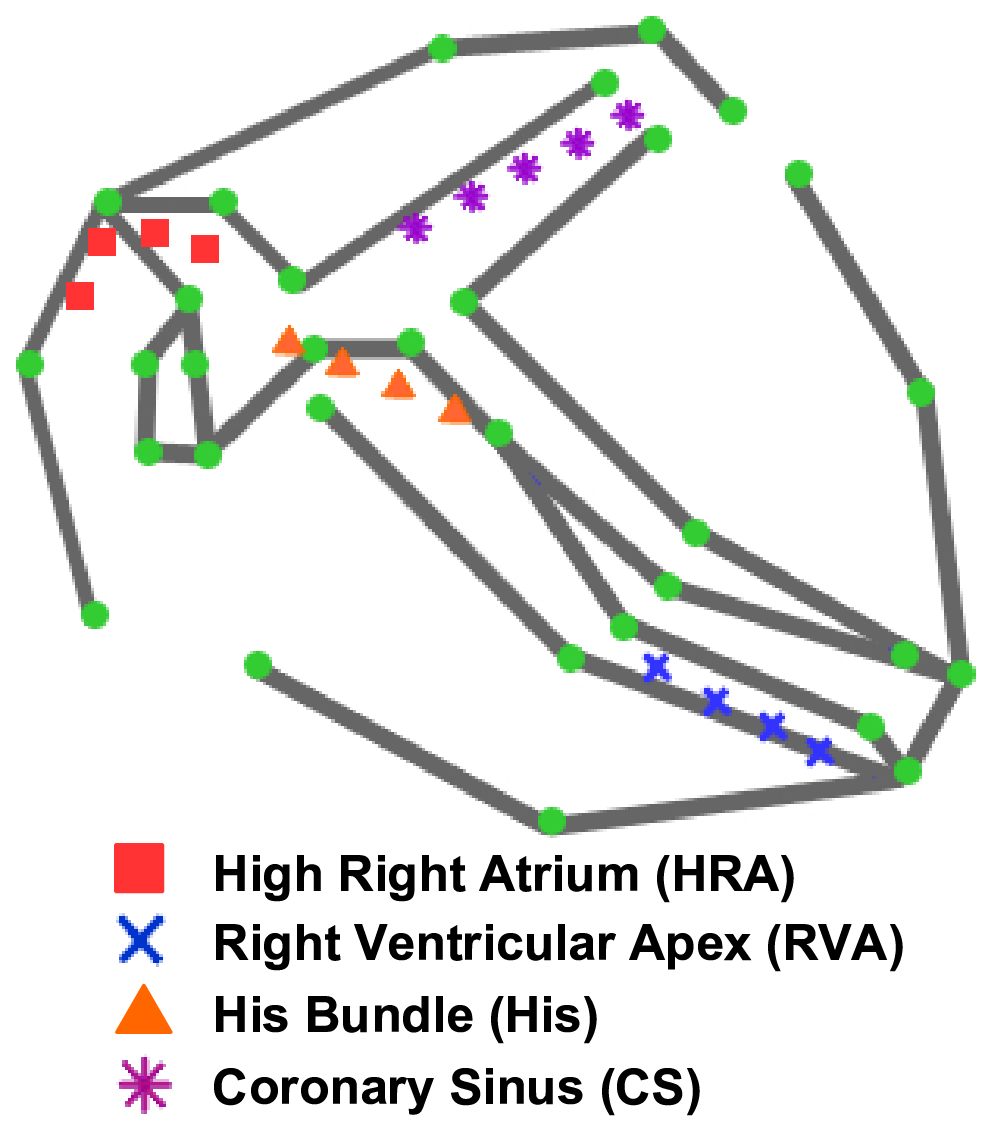
\includegraphics[width=0.25\textwidth]{figs/gen_setup.png}
		%\label{fig:general_setup}
		%} 

%\vspace{-10pt}
\caption{\small (a) Node automaton: The dotted transition is only valid for tissue (like SA node) that can be activated by an external trigger; (b) Path automaton modeling the electric conduction and propagation between two node automata; (c) Electrical conduction system of the heart; (d) Model of the electrical conduction system of the heart using a network of node \& path automata (~\cite{VHM_proc}).}\label{fig:automata}
%\vspace{-15pt}
\end{figure} 

Due to the limited number of observable points within the heart, modeling the electrophysiological behavior of every tissue of the heart and its full anatomy is unnecessary and unfeasible. In our heart models, only self-activating tissue and key hubs of the electrical conduction system are modeled as node automata. 

\textbf{Path Automata:} The electrical conduction through the tissue between nodes are abstracted using \emph{path automata}. The path automata can be used to represent structural or topological (functional) electrical connections between nodes. \figref{automata}.(b) shows a path automaton connecting node a and b.

The initial state of a path automaton is \emph{Idle}, which corresponds to no conduction. The states corresponding to the two conduction directions are named after the physiological terms: Antegrade (Ante) and Retrograde (Retro). These states can be intuitively described as forward and backward conductions. If path actuation \emph{Act\_path} event is received from one of the nodes connected to it, there is a transition to \emph{Ante} or \emph{Retro} state based on the activation source in the path automaton. At the same time, the clock invariant of the state is modified according to the shared variable \emph{C(a/b)}. This corresponds to the change of the conduction delay that is caused by the early activation. Similar to node automaton, the changing trend is extracted from clinical data and the function $h$ is defined as:
\begin{equation} 
						h(c) = \left\{
						\begin{array}{lr}
						
						path\_len/v\cdot (1+3c), i=AV\\
						path\_len/v\cdot (1+3c^2), i\neq AV
						\end{array}
						\right.
						\end{equation}
where $path\_len$ denotes the length of the path and $v$ is the conduction velocity.

After \emph{Tante} or \emph{Tretro} time expires, the path automaton sends out \emph{Act\_node(b)} or \emph{Act\_node(a)} respectively. A transition to \emph{Conflict} state occurs followed by the transition to \emph{Idle} state. The intermediate state \emph{Conflict} is designed to prevent back-flow, where the path is activated by the node \emph{b} it has just activated. If during \emph{Ante} or \emph{Retro} state another \emph{Act\_path} event is received from the other node connected to the path automaton, a transition to \emph{Double} state will occur, corresponding to the two-way conduction. In this case, the activation signals eventually cancel each other and the transition to \emph{Idle} state is taken.

\subsection{Modeling the Heart's Electrical Conduction System}
The node and path automata are the basic building blocks for EP heart modeling. Hearts with different conditions are modeled by using different conduction topologies with appropriate timing parameters for each node and path automata. \figref{automata}.(d) shows one such topology of a network of node and path automata.

\section{Interaction with the Heart Model}
In this section, we first introduce a probe model we developed to generate synthetic EGM signals from the EP heart model.
We then use two case study to demonstrate that the probe model enables the EP heart model to evaluate device malfunctions due to sensing errors.
\subsection{Probe Model for Synthetic EGM Generation}
In EP testing and during pacemaker implantation, the local electrical activities, measured as electrogram (EGM) signals, are used to diagnose heart conditions. 
During heart model construction, we can assign a node automaton at electrode locations and the transitions to the ERP state can be used to represent the local activation events. 
In a more general setup where electrodes are assigned anywhere within the heart model, a probe model is designed to generate synthetic EGM signals using spatio-temporal information from the proximity to the network of node and path automata. 

According to \cite{recording}, a potential difference is generated when the activation wavefront passes by the electrode. 
The locations of the activation wavefronts are calculated from the locations of the path automata and their current timer values. 
The amplitude of EGM decreases when the activation wavefront moves away from the probe. 
We assume the decrease factor is a function related to the distance between the activation wavefront and the probe. 
The potential difference caused by an activation wavefront to a probe is the signal strength of the path multiplied by the decrease factor. 
The amplitude of EGM from a probe is the sum of potential differences caused by all activation wavefronts. 
The bipolar EGM is the difference between two unipolar EGMs. 
\figref{egm_s} shows that this probe model captures timing properties of EGM and the functional shape of the EGM impulses. 
The probes can be placed anywhere within the heart model and generate clinically-relevant EGMs. 
\begin{figure}[!t]
\center
%\vspace{-15pt}
		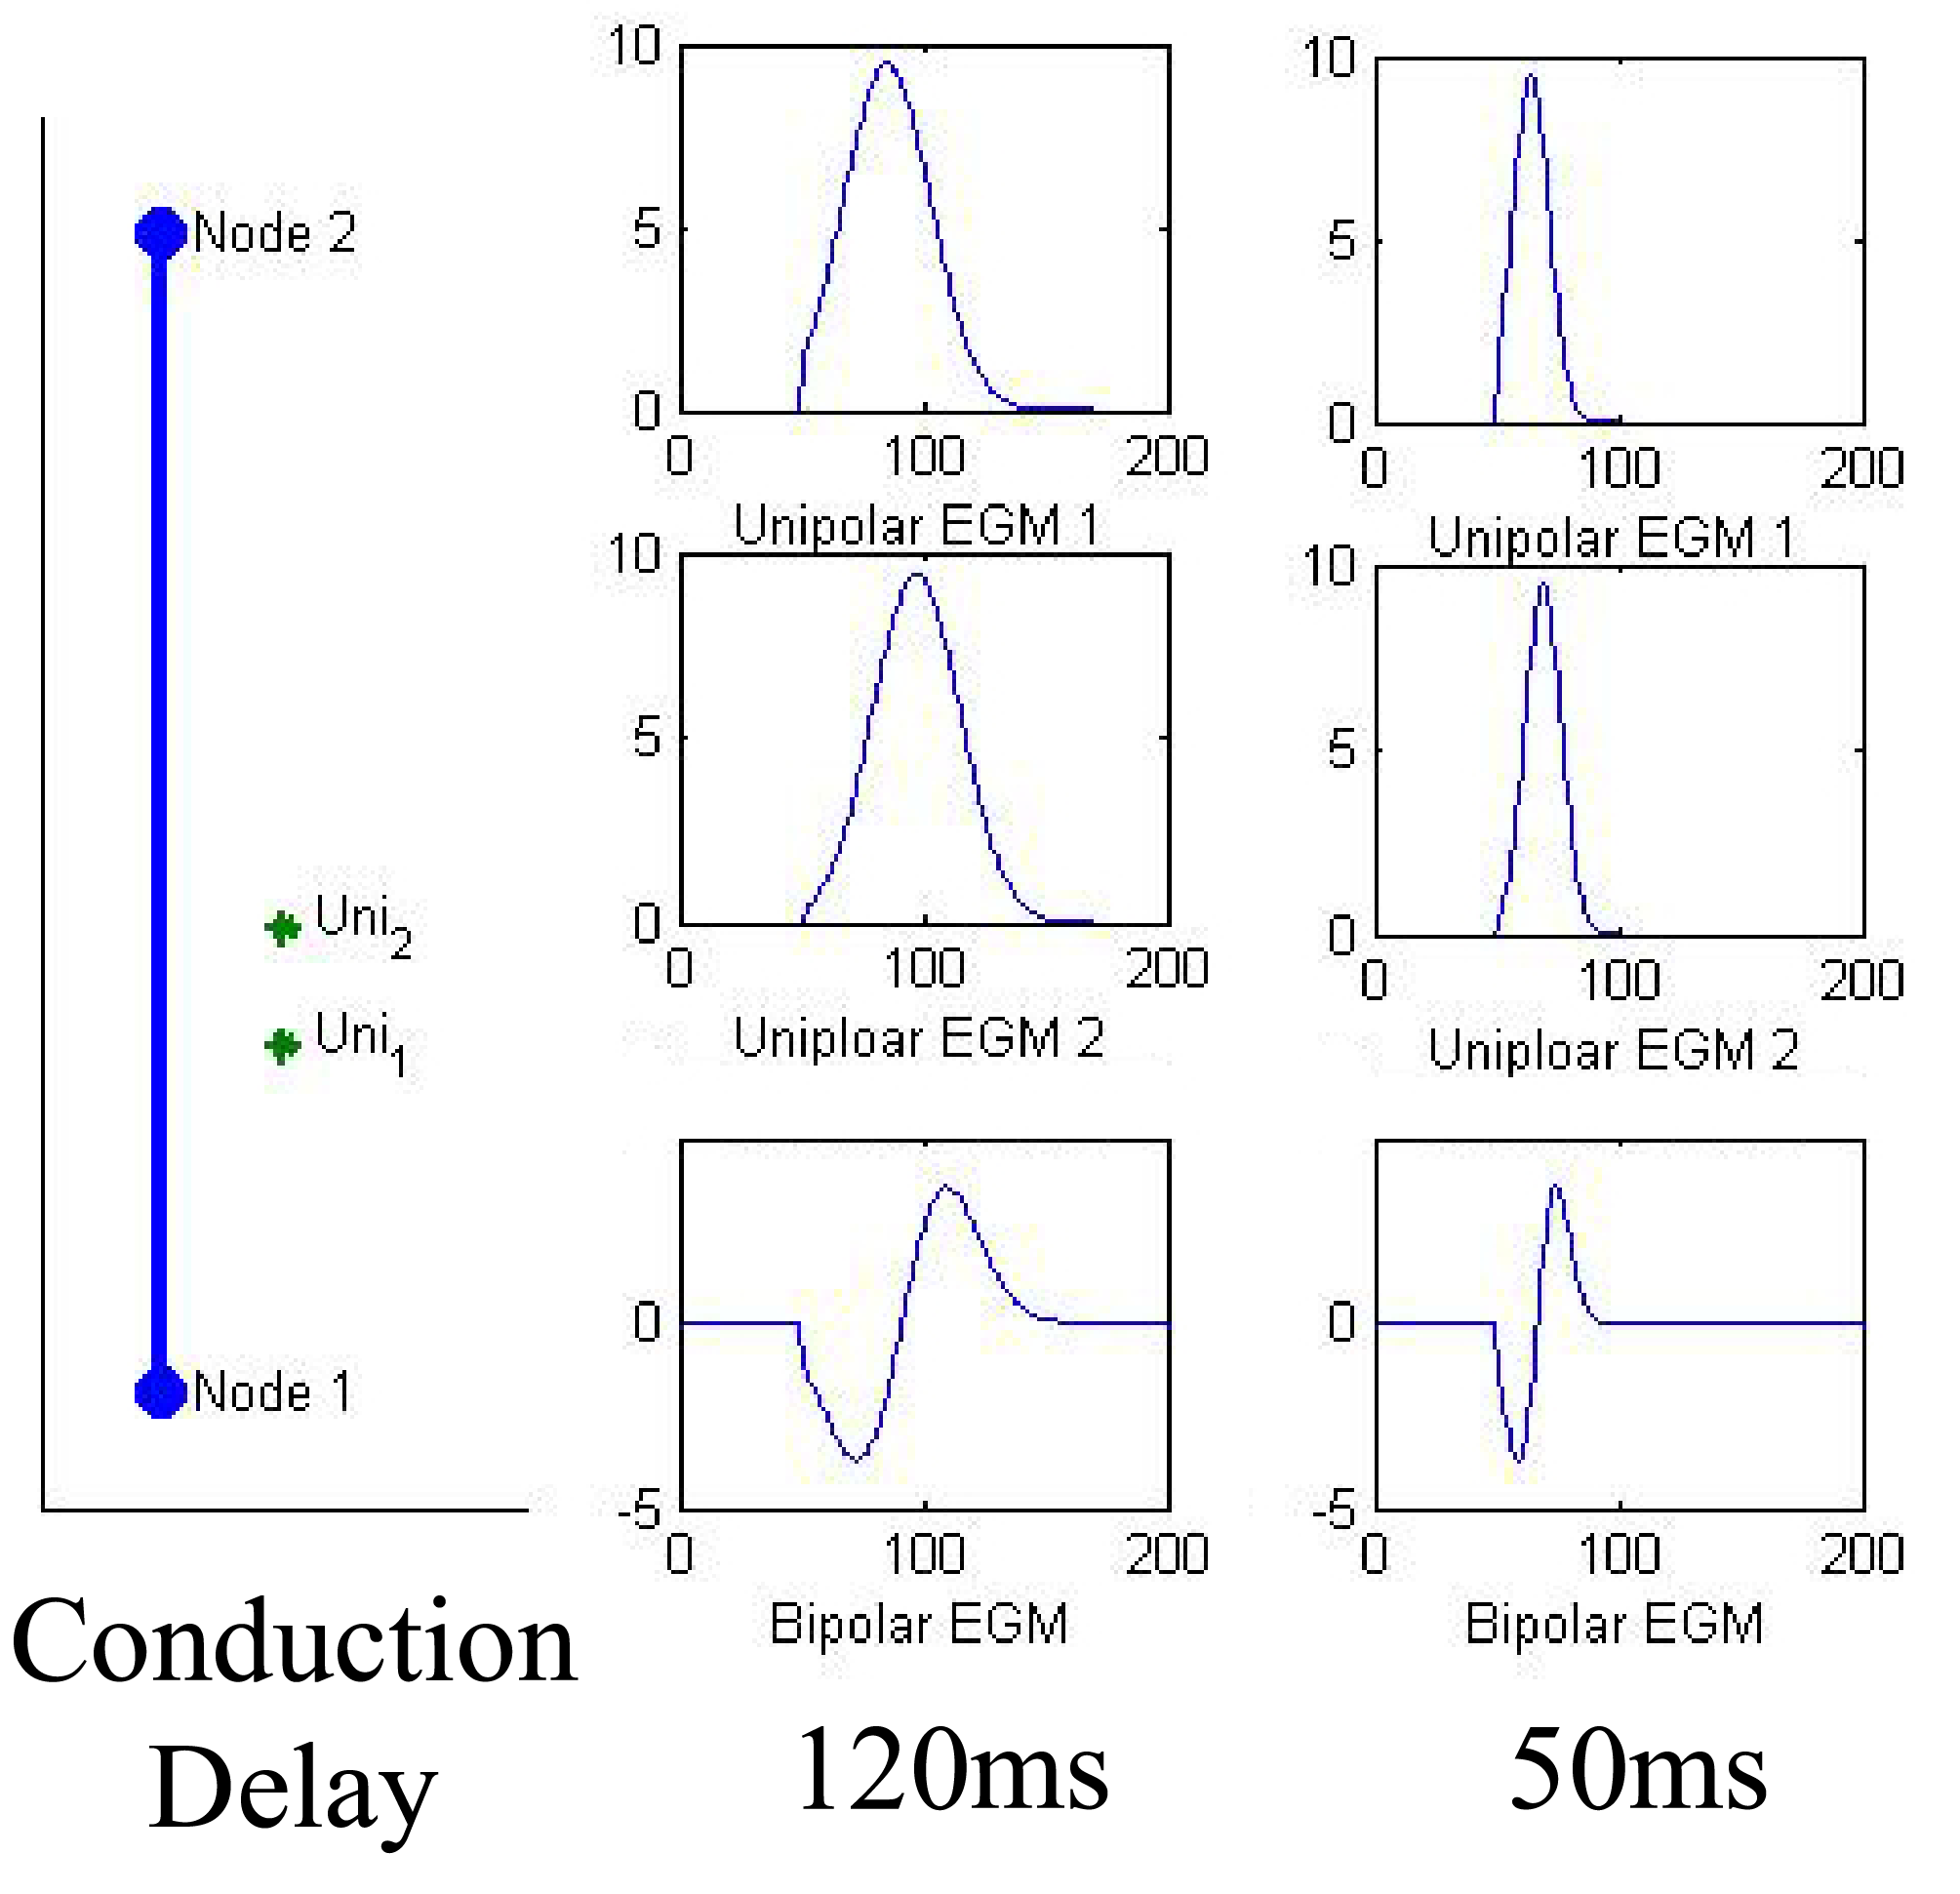
\includegraphics[width=0.7\textwidth]{figs/fig7.png}
%\vspace{-10pt}
\caption{The influence of conduction velocity and probe configuration on the EGM morphology. The left columns show the placement of probes in relation to the path; the right columns show the functional EGM.}
\label{fig:egm_s}
%\vspace{-15pt}
\end{figure}


\begin{figure}[t]
\center
		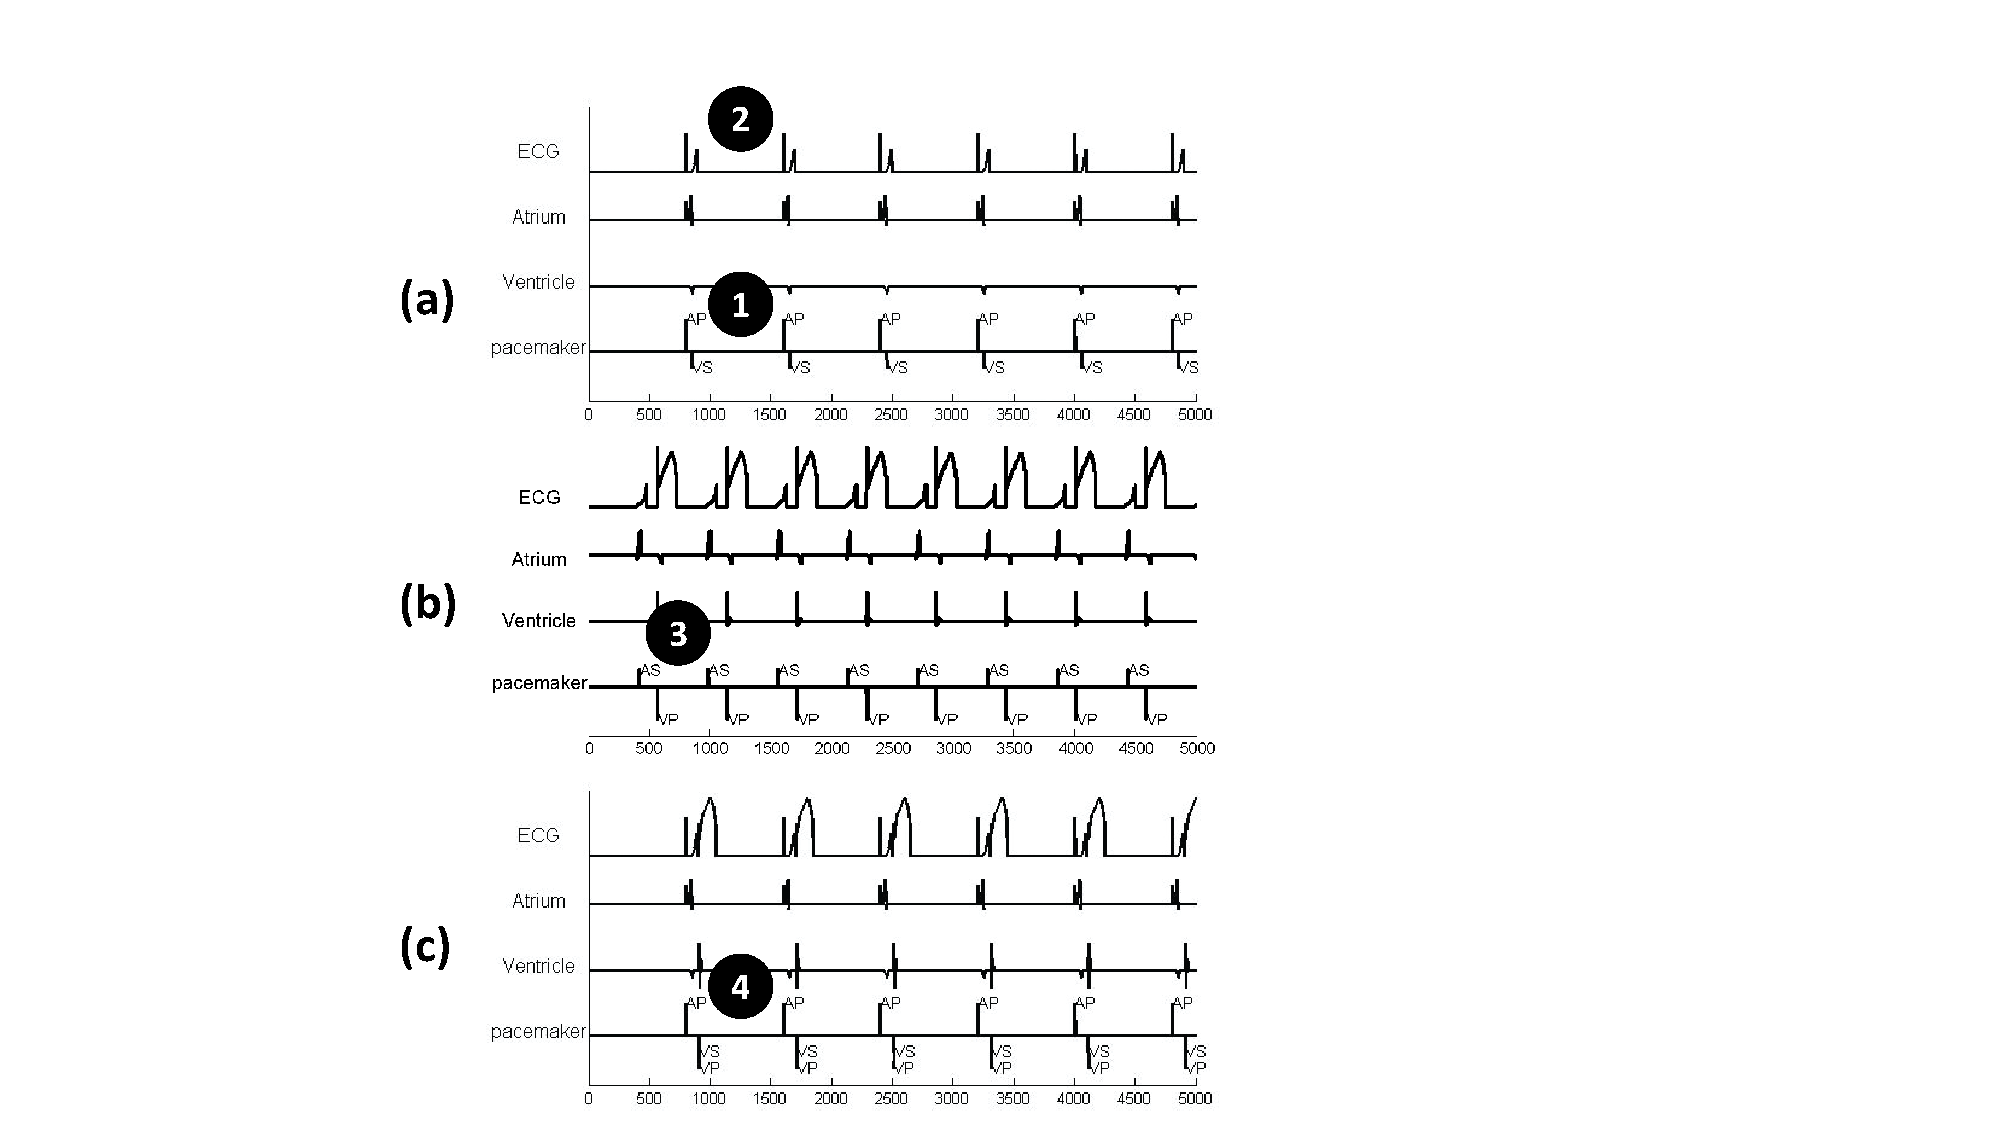
\includegraphics[width=0.6\textwidth]{figs/crosstalk_all.pdf}
%\vspace{-20pt}
\caption{Crosstalk between pacemaker leads with high sensitivity in the ventricle, adjusted sensitivity and ventricular safety pacing}
\label{fig:crosstalk}
%\vspace{-15pt}
\end{figure}
With the sensing model, the heart model structure can be used to identify safety hazards caused by sensing errors.
\subsection{Pacemaker Oversensing and Crosstalk}
Oversensing is a general term for inappropriate sensing caused by noise or far-field signals.
 It's very common among pacemaker malfunctions and it may result in failure to pace (\cite{med2, leads}), competitive pacing and inappropriate therapy. 
Crosstalk is a special case for oversensing which occurs when the pacemaker stimulus in one chamber is sensed in the other chamber. 
It happens when two leads are close to each other or pacing signal in the other chamber is too strong. 
It is common that the ventricular lead is placed in the right ventricle outflow tract, which is close to the atrium (\cite{icd}). 
\figref{crosstalk}(a) shows simulated EGMs from a patient with bradycardia and complete heart block. During atrial pacing (AP), the pacing signal is sensed by the ventricular lead 53 ms after the AP. (Marker 1) 
It is treated as ventricular sense (VS) signal and thus inhibits the subsequent ventricular pacing (VP). 
This is indicated by no QRS-wave in the ECG channel. (Marker 2) For a patient with complete heart block this will cause dangerous ventricular asystole, meaning a long time without ventricular events.  

Increasing the sensing threshold of the ventricular channel can prevent false sensing. 
In \figref{crosstalk}(b), the small signals in ventricular EGM are ignored and ventricular pacing are successfully delivered. 


%%%%%%%%%%%%%%%%%%%%%%%%%%%%%%%%%%%%%%%%%%%%%%
\begin{figure}[t]
\centering
		%\subfigure [\small]{
		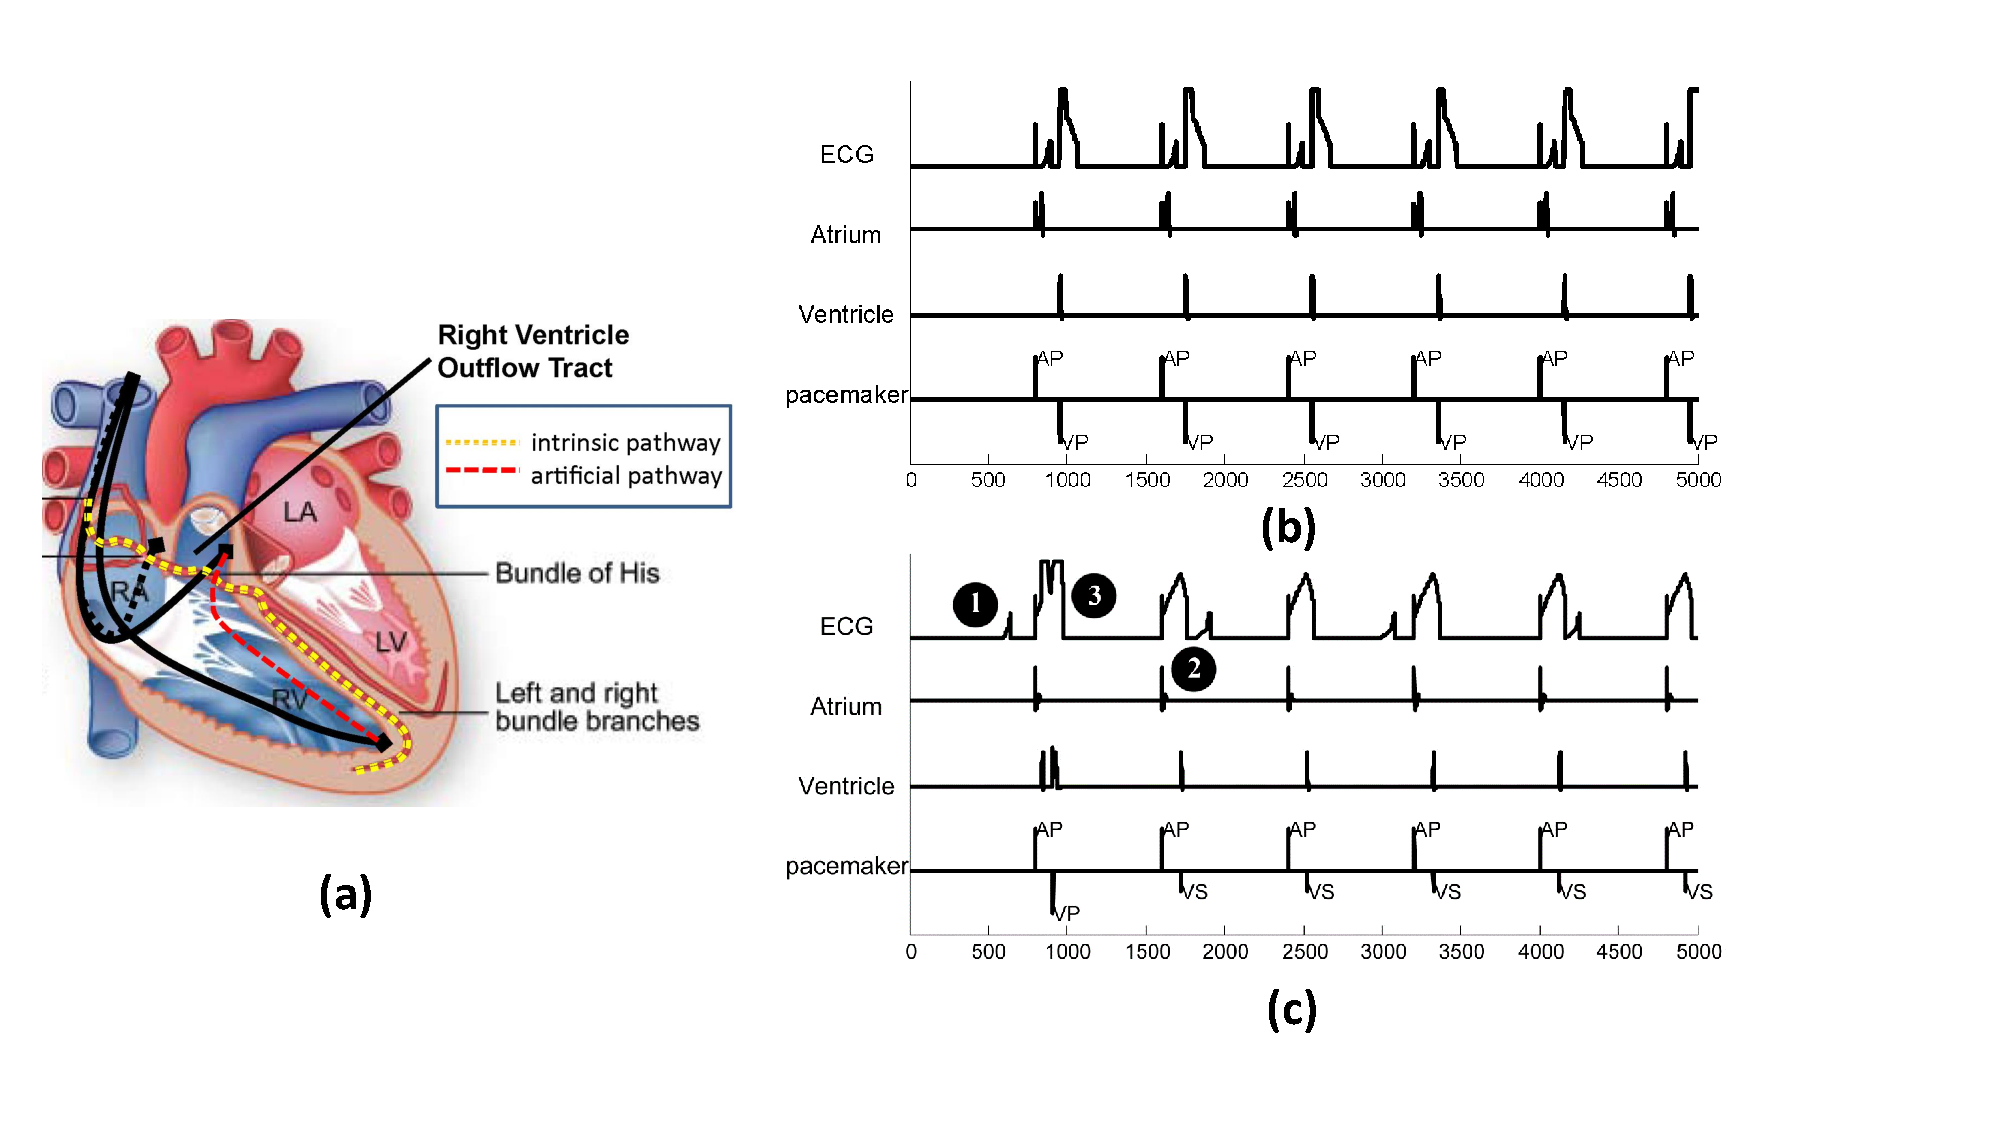
\includegraphics[width=\textwidth]{figs/dislodge_all.pdf}
		%} 
		%\subfigure [\small]{
		%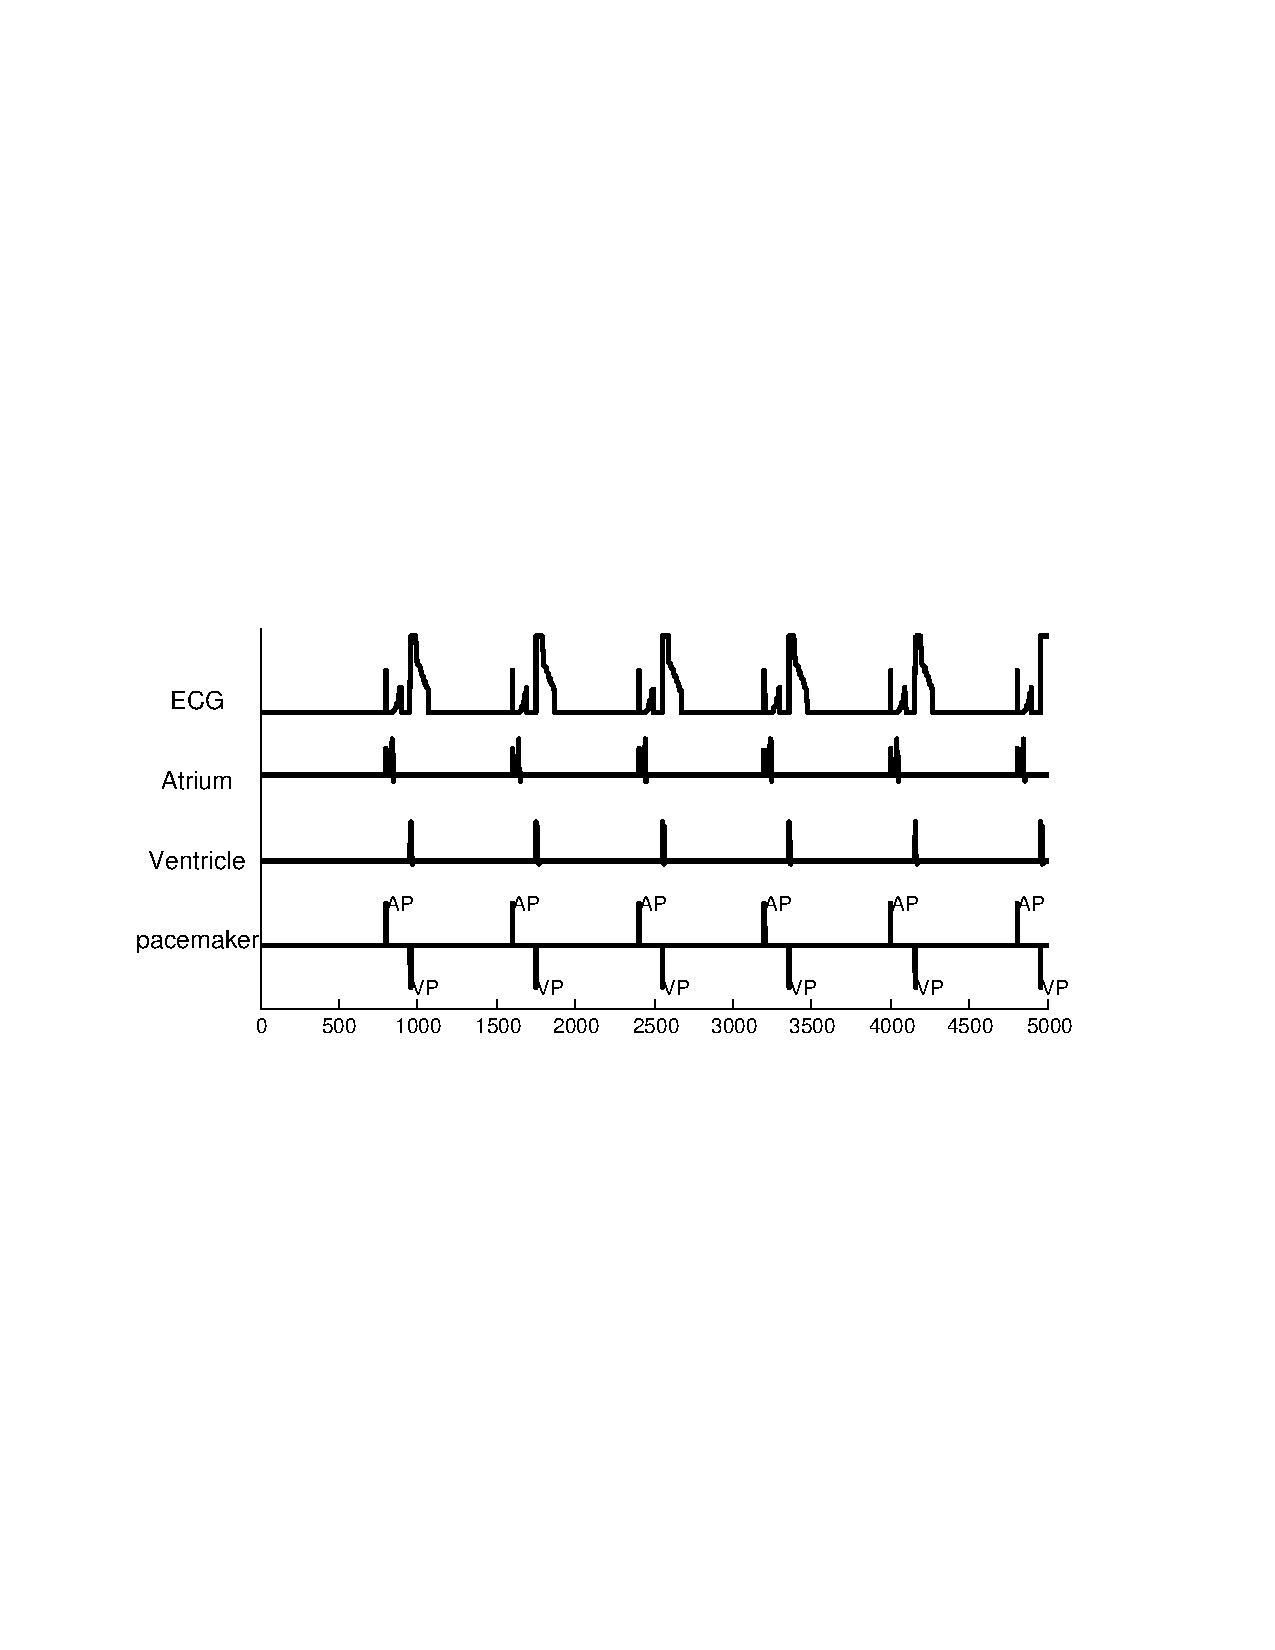
\includegraphics[width=0.36\textwidth]{figs/dislodge_norm.pdf}
		%\label{fig:dislodge_norm}
		%} 
		%\subfigure [\small] 
		%{
		%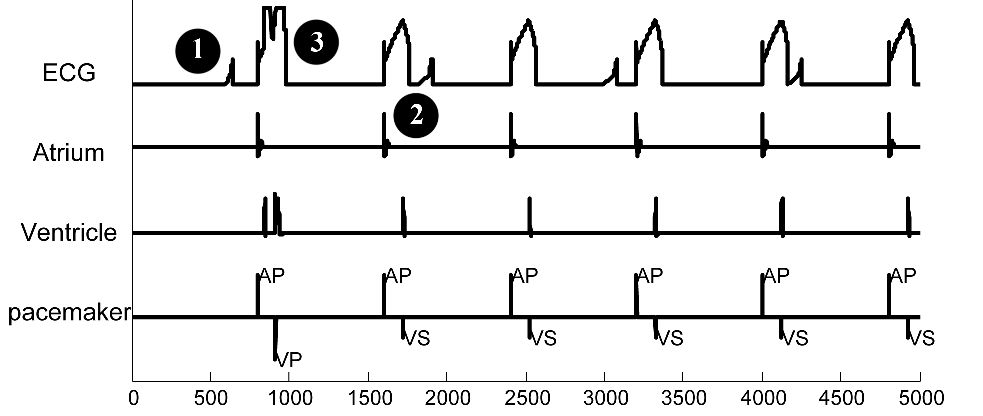
\includegraphics[width=0.36\textwidth]{figs/dislodge_new.pdf}
		%\label{fig:dislodge}
		%} 
%\vspace{-5pt}
\caption{\small (a) Dotted line shows the location where the atrial lead should be (b) Pacemaker function before lead dislodge. (c) Pacemaker function after lead dislodge}
		\label{fig:dislodge_all}

%\vspace{-15pt}
\end{figure} 
%%%%%%%%%%%%%%%%%%%%%%%%%%%%%%%%%%%%%%%%%%%%%%


\subsection{Lead Displacement}
Lead displacement affects many patients and can result in inappropriate or ineffective therapy. 
\figref{dislodge_all}. (b) shows the simulation result for the pacemaker function when the leads are in their designated location. 
From the figure we can observe: 1) Each P-wave is initialized by an Atrial Pace signal. 2) Each QRS complex is initiated by a ventricular pacing signal. 3) The interval between AP and VP is 150 ms, which matches the programed AVI period.

%%%%%%%%%%%%%%%%%%%%%%%%%%%%%%%%%%%%%%%%%%%%%%
 %\begin{figure}
%\center
%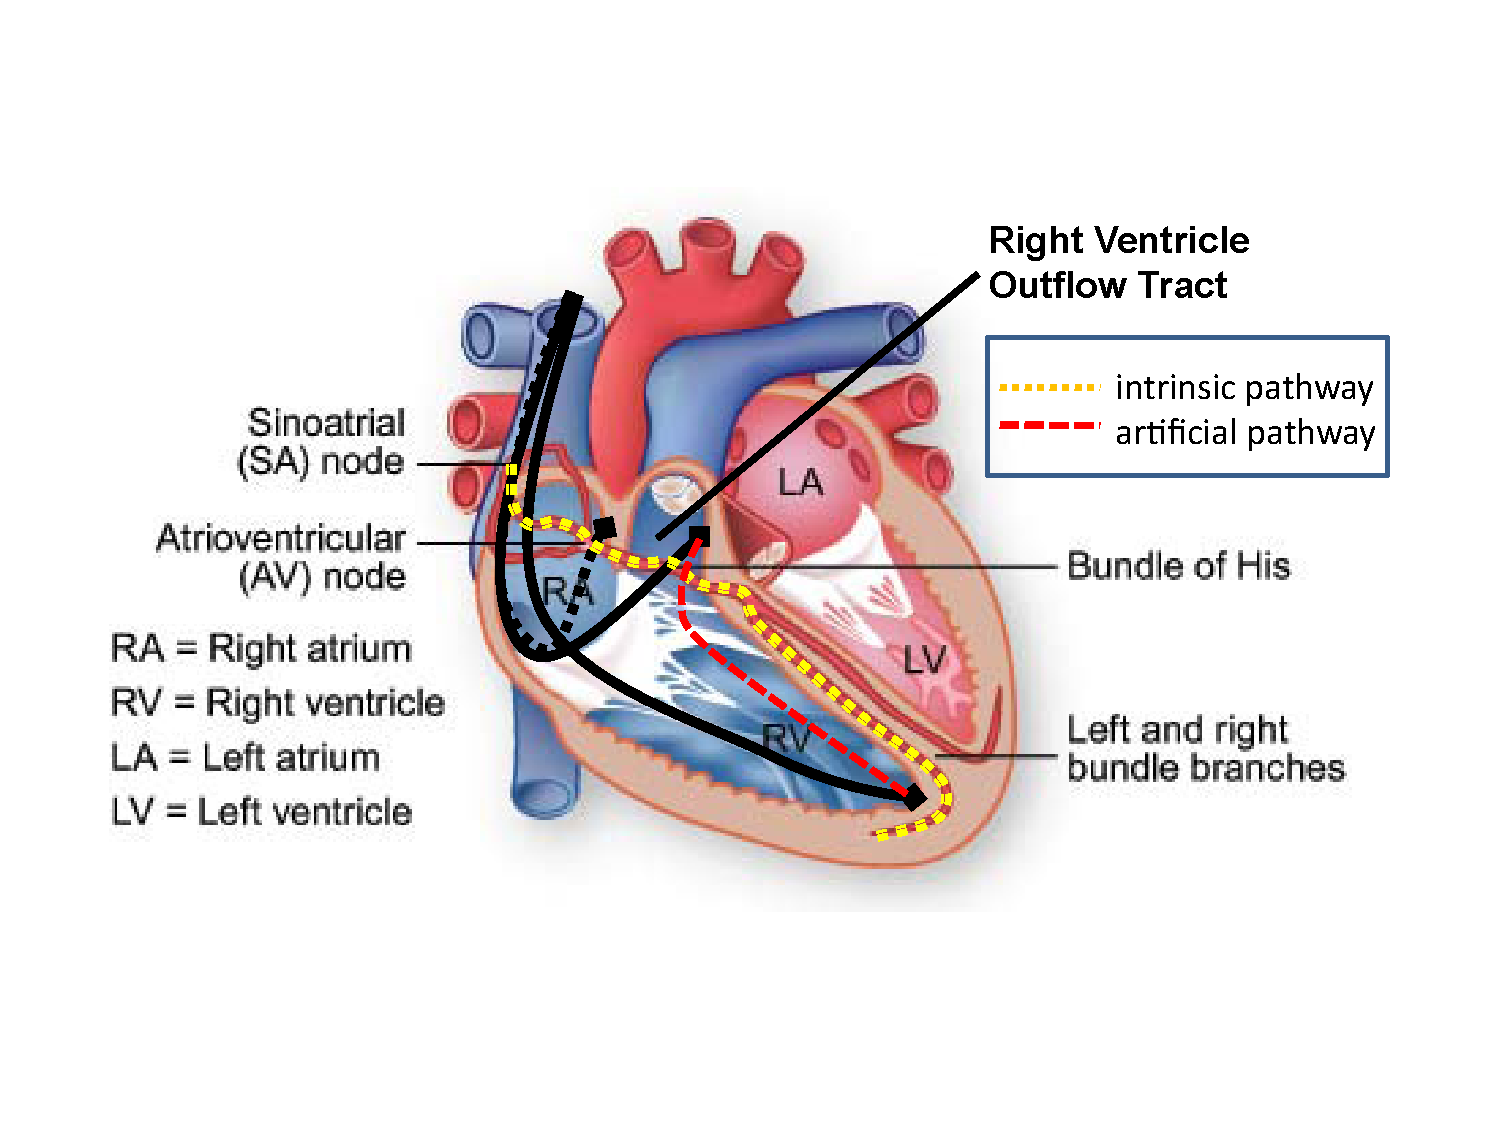
\includegraphics[width=0.7\textwidth]{figs/race_cond.pdf}
%\caption{Dotted line shows the location where the atrial lead should be}
%%\vspace{-15pt}
%\label{fig:race_cond}
%\end{figure}
%%%%%%%%%%%%%%%%%%%%%%%%%%%%%%%%%%%%%%%%%%%%%%

One common case for lead dislodge is shown in \figref{dislodge_all}.(a), where the atrial lead has fallen into the right ventricle outflow tract. 
In this case the atrial lead senses from the ventricle rather than atrium and atrial pacing will initiate a ventricular event.
 \figref{dislodge_all}.(c) shows the simulated EGMs in this case. 
The figure reveals several facts: 1) No P wave is sensed or tracked (Marker 1). 2) Atrial Pace initiates an abnormal, wide QRS which is then sensed by the ventricle lead (Marker 2). 3) Intermittent appearance of VP on QRS 110 ms after the AP. 
The ventricular lead can receive signal from: 1) pacing signal sent from the atrial lead, 2) the intrinsic A-V conduction path. The two paths are shown in \figref{dislodge_all}.(a) and form a timing race condition. When the signal from the atrial lead arrives the ventricular lead first, it will trigger VS. If the intrinsic signal arrives the ventricular lead during the VSP sensing window (defined in previous section), it will trigger VSP. Although the pacing is 'safe' because the pacing is early enough to avoid the vulnerable refractory period, the damage caused by pacing on depolarized tissue is currently a matter of much investigation.\\



\section{Heart-on-a-Chip Platform}
\begin{figure}[!t]
\center
%\vspace{-15pt}
		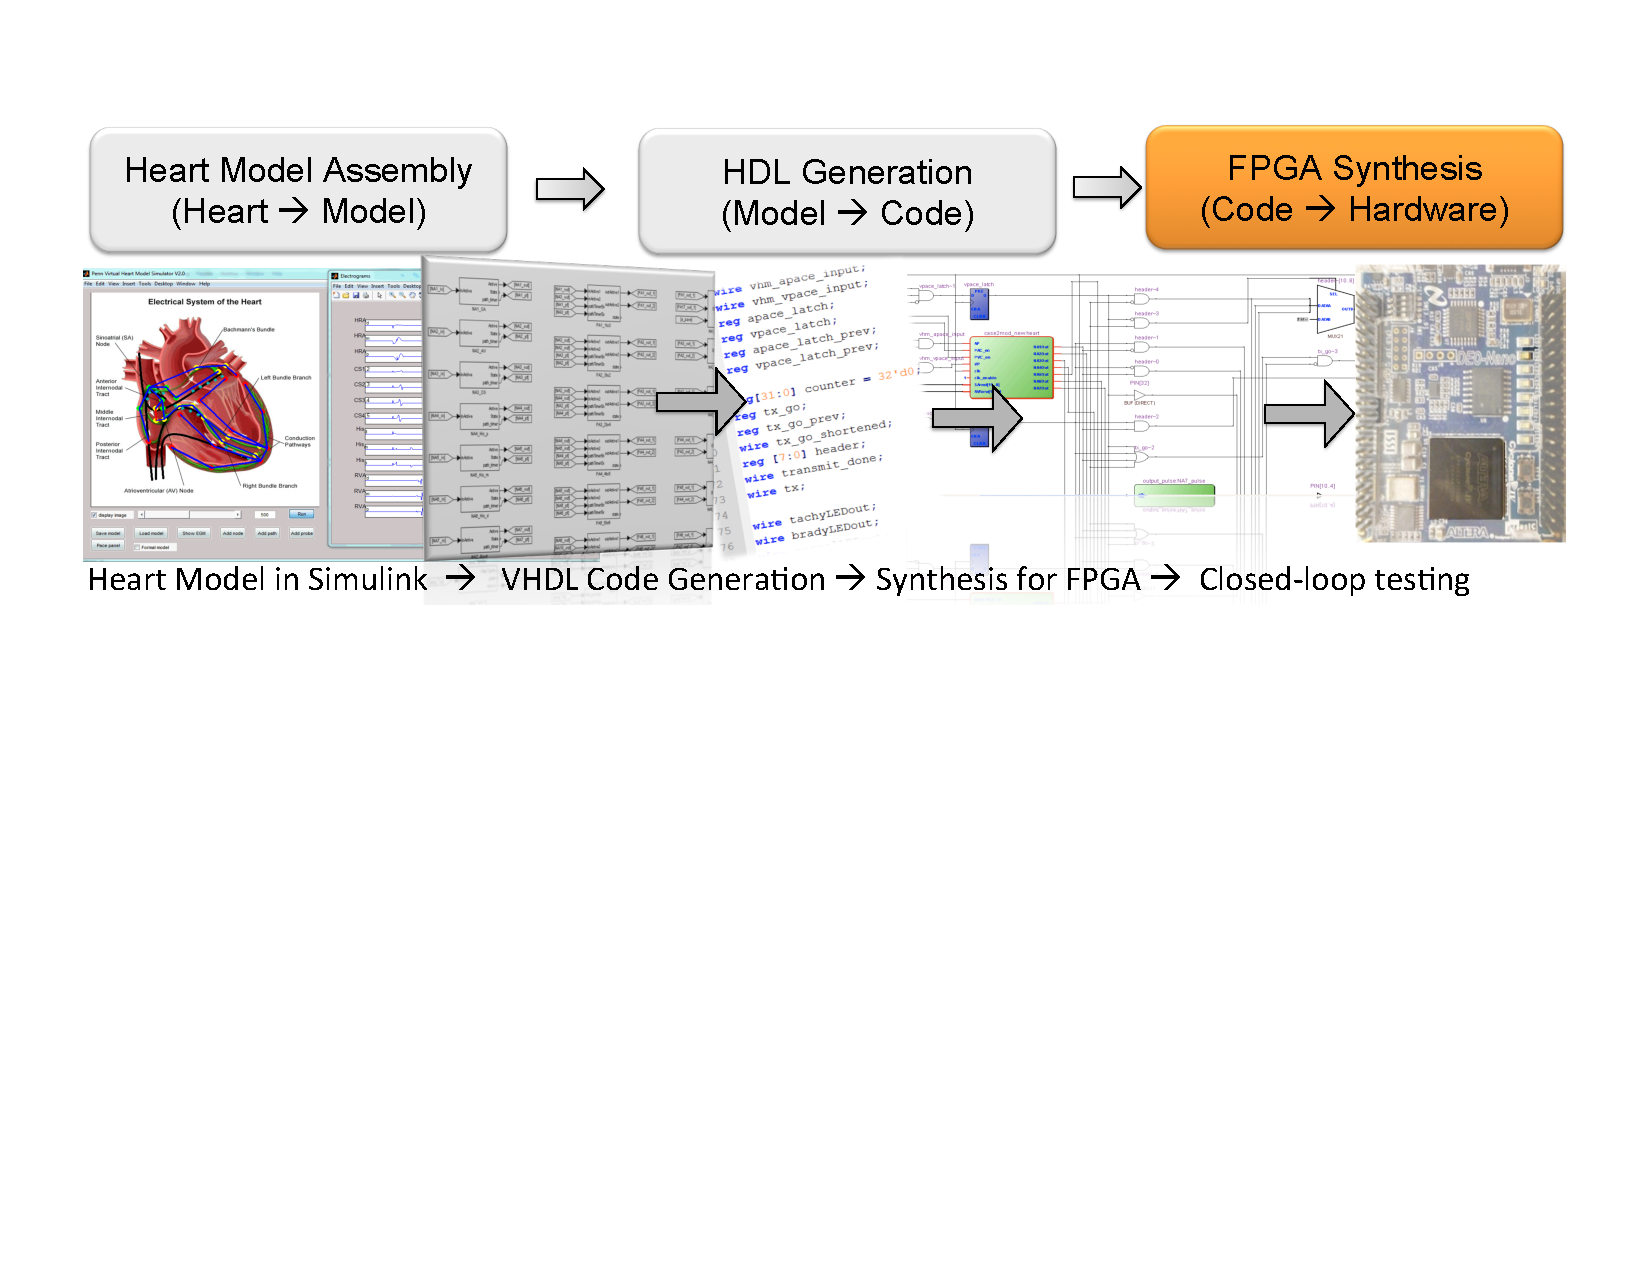
\includegraphics[width=0.98\textwidth]{figs/modeling_heart.pdf}
%\vspace{-10pt}
\caption{The heart model was developed in Matlab/Simulink and code was automatically generated to operate on an FPGA platform for platform-level testing.}
\label{fig:modeling_heart}
%\vspace{-15pt}
\end{figure}
The heart model structure is also available  on hardware platform (\figref{modeling_heart}) for closed-loop testing of pacemaker implementations. 
Since each heart model is a network of node and path automata running concurrently, we implemented the heart model on an FPGA, so that increasing in the number of nodes and paths would not affect real-time constraints. 
The second generation heart model implementation has been implemented on a lower cost fast micro-controller platform. 
The fast clock ensures that executions of all nodes and paths can be finished within 1ms. 
The Heart-on-a-Chip platform includes a heart model implementation which is able to represent common heart conditions such as bradycardia, tachycardia, heart block, etc (for mode details refer to \cite{VHM_proc}). 
The parameters of the heart model can be changed at run-time by either switching among pre-defined parameter sets, or sending values directly to the model through a user interface in Matlab. 
A monitoring system observes logical interactions between heart model and the pacemaker and checks them against safety invariants at run-time. 

As shown in (\figref{HOC}), with an analog interface the heart model can interact with a commercial pacemaker in real time. 
Our analog interface uses an optical isolation circuit to separate the pacemaker circuit and the heart implementation. 
Signals generated from the heart are attenuated to the appropriate level to interact with a Boston Scientific pacemaker and analog pacing signals are converted to pacing events received by the heart model. 

\begin{figure}[!b]
\center
%\vspace{-15pt}
		\includegraphics[width=0.8\textwidth]{figs/PVS.pdf}
%\vspace{-10pt}
\caption{Heart-on-a-Chip testbed for real-time closed-loop testing of the pacemaker or model of the pacemaker with the heart model on the hardware platform}
\label{fig:HOC}
%\vspace{-15pt}
\end{figure}

% \subsubsection{Abstracting Beat-to-beat Dynamics}
% \subsubsection{Abstracting Conduction Delays with Path}
% \subsubsection{Merging Activation-generating Nodes}
% \subsubsection{Replace ERP Blocking With Non-deterministic Conduction}
% \subsubsection{Replace }





\section{EP Heart Model Validation}
%The validity of the environment models affects the validity of the closed-loop verification results. 
Since models are approximations of the actual environment, there are always discrepancies between the model and the actual patient (group). 
The validity of closed-loop validation results directly correlated to the validity of the physiological models.

In this section we validate the heart model structure by demonstrating its capability to represent physiological behaviors of 1) a particular patient for closed-loop simulation, and 2) a group of patients for closed-loop model checking.
The metrics and process to validate the heart model are different for the two applications of heart modeling: in closed-loop simulation, the \textbf{accuracy} of the model is more important, while in closed-loop model checking, the model's \textbf{coverage} on environmental behaviors is more important.



\subsection{Validating Models for Closed-loop Simulation}
A physiological model is considered valid for closed-loop simulation if (a) it is capable of generating the same output as the patient, for the same input; and (b) it is general enough to represent other patients with similar conditions by adjusting its parameters. The second point is to ensure that the model successfully captures the underlying mechanism instead of over-fitting the data. In the following example we validate the capability of our heart models to represent certain heart conditions according to the mechanisms described in physiological literature, and  output the correct responses across a range of inputs.\\

%To use a physiological model for closed-loop simulation, there are two levels of validity: 1) model a patient with certain heart condition, 2) model a \em ph{specific} patient with certain heart condition. Level 1 validity ensures that the model successfully models the underlying mechanism of the heart condition, while level 2 validity guarantees the capability of the model to generate same data as the corresponding patient given the same input. Note that satisfying level 2 without satisfying level 1 may result in over-fitting.
\begin{figure}[!t]
\centering
		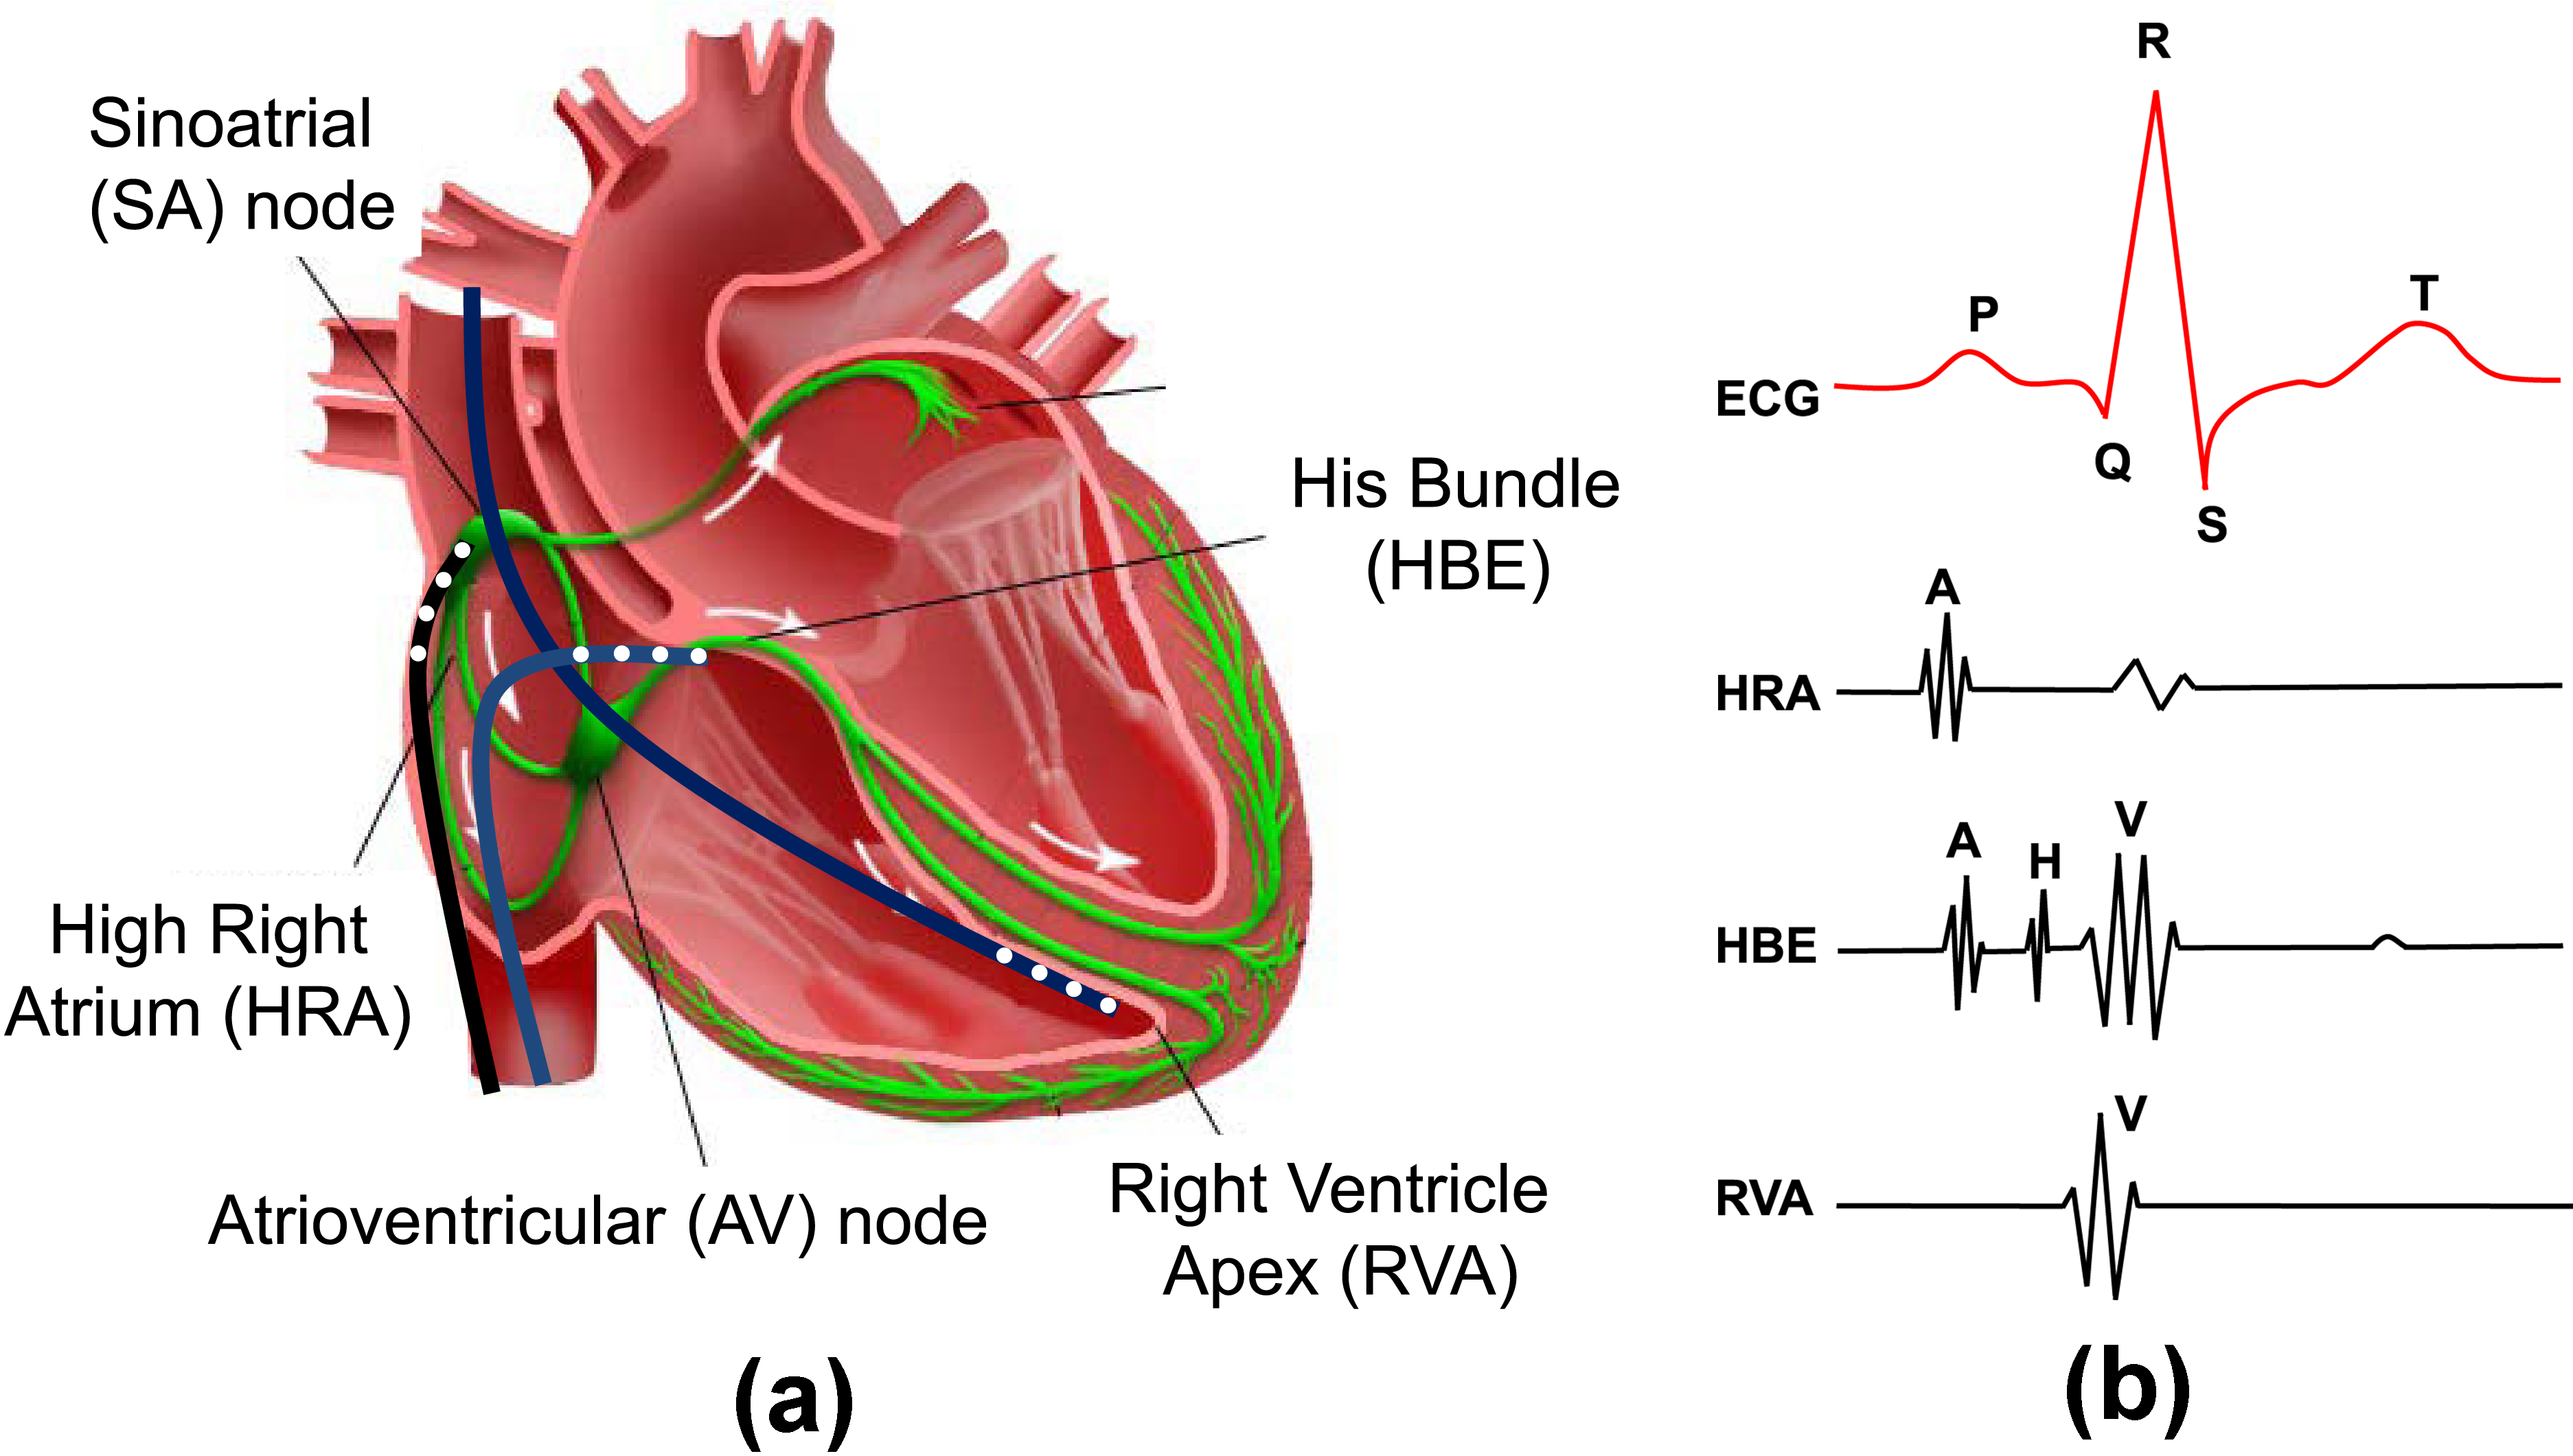
\includegraphics[width=0.95\textwidth]{figs/probes.png}
		
%\vspace{-10pt}
\caption{\small (a) Probe locations for a general EP testing procedure. (b) EGM signals measured from the probes at the high right atrial (HRA), His bundle (HBE) and right ventricular apex (RVA) standard catheter positions}
\label{fig:egm}
%\vspace{-15pt}
\end{figure} 

\noindent\textbf{Quantitative Heart Model Validation:} During an EP testing procedure, the physician places catheters inside the patient's heart to observe local electrical activity from different locations of the heart. The His bundle catheter (HBE) is particularly important when evaluating the atria-to-ventricle conduction path (\figref{egm}). For each A to V conduction there are 3 impulses which correspond to atrial contraction (A), His bundle activation (H) and ventricular activation (V).  In this case study, two pacing signals $a1$ and $a2$ are delivered to the heart from the high right atrial catheter (HRA). By gradually decreasing the pacing interval in each test, certain tissue along the A-V conduction path will be activated during its refractory period, thus affecting the conduction delay further down the conduction path and change the intervals between the impulses. \figref{book_1} shows the relation between pacing interval ($a1$-$a2$) and corresponding intervals between A, H and V impulses. On the left side it shows that interval $H_1-H_2$ and $V_1-V_2$ decrease but remain equal as the pacing interval decreases, indicating the tissue with the longest refractory period along the path is not between the His Bundle and the ventricles. When the pacing interval decreases to 350ms both intervals increases, indicating that the RRP of certain tissue has been reached and the tissue is between the atria and the His bundle. On the right it shows that the $A_2-H_2$ interval increases as the pacing interval decreases, which further proves the hypothesis that the AV node, which is between the atria and the His bundle, has the longest refractory period along the A-V conduction path. We configured our heart model such that the AV node has the longest refractory period and performed the same study by decreasing the pacing interval. The heart model shows the same trend as that of the real patient (\figref{type_1}).
\begin{figure*}[!t]
\centering
		\subfigure 	[\small] 
		{
		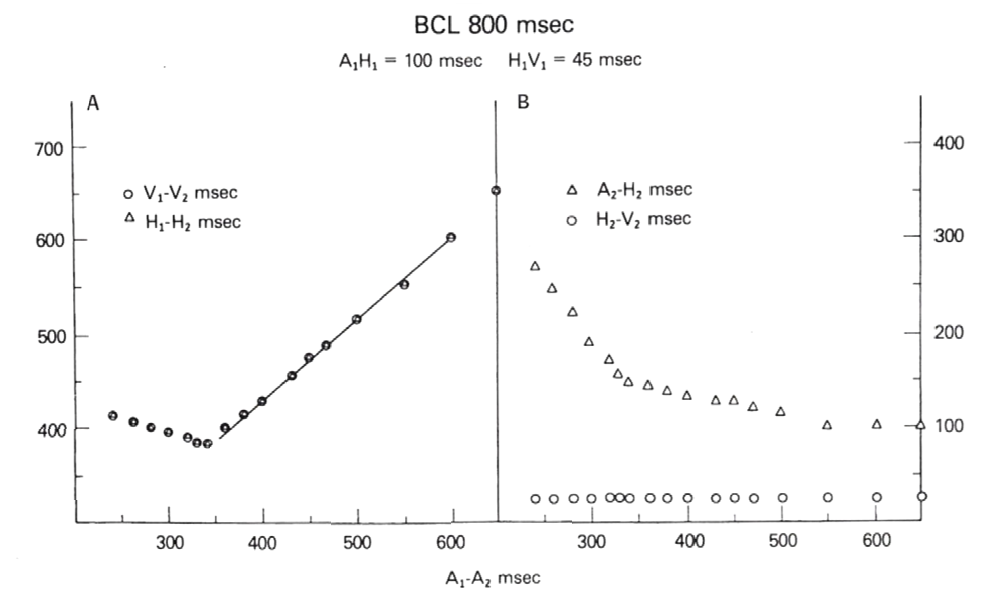
\includegraphics[width=0.95\textwidth]{figs/book_1.png}
		\label{fig:book_1}
		} 
		\subfigure [\small ] 
		{	
			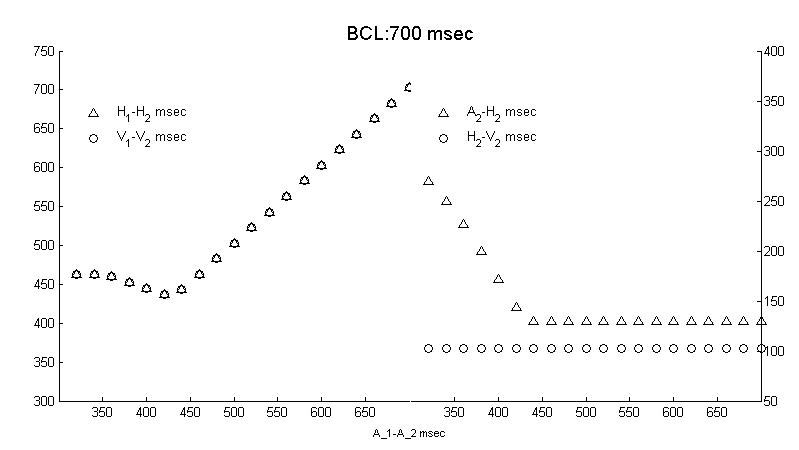
\includegraphics[width=0.9\textwidth]{figs/type_1.png} 
			\label{fig:type_1}
		}
\label{fig:Case_1}
%\vspace{-5pt}
\caption{\small Key interval values when the coupling interval shortens for (a) a real patient (\cite{josephson}) and (b) in heart model simulation (\cite{vhm_ecrts10}).}
%\vspace{-15pt}
\end{figure*} 


% \begin{figure}[\b]
% 	\center
% 	\vspace{-20pt}
% %	\includegraphics[width=0.49\textwidth]{figs/AV_reentry_circuit.pdf}
% 	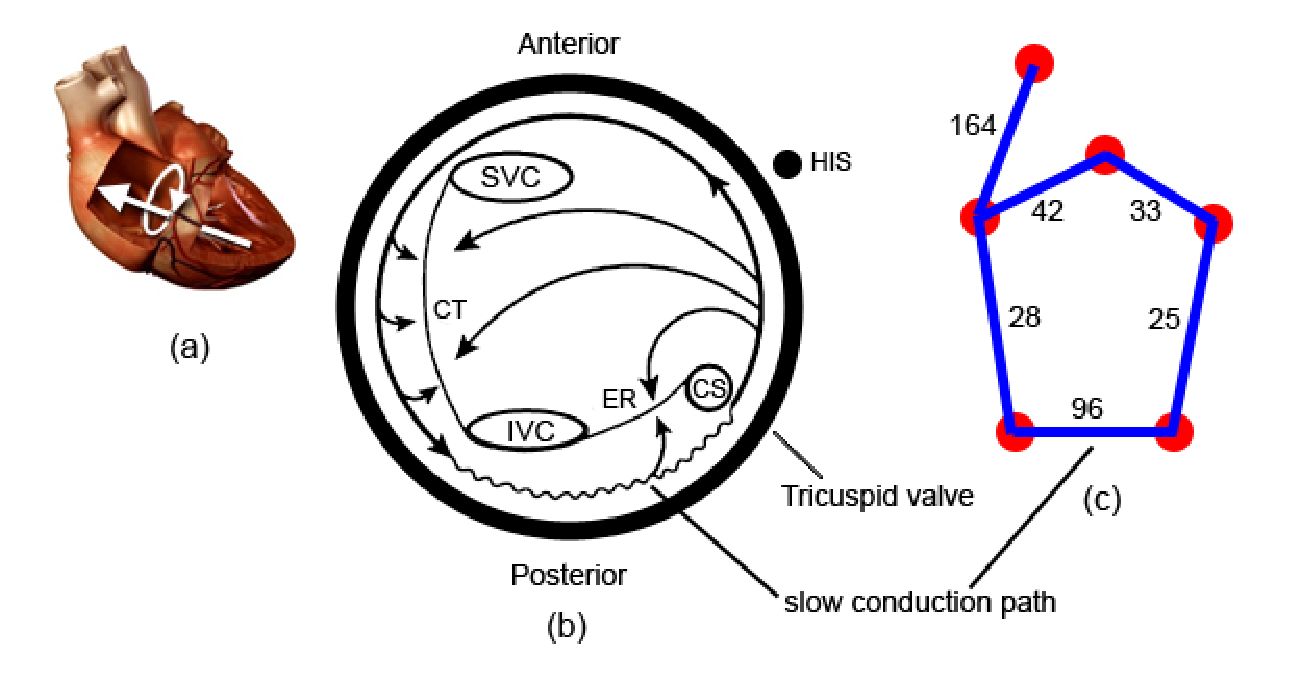
\includegraphics[width=0.5\textwidth]{figs/AFL_circuit.pdf}
% 	\center
% 	\vspace{-15pt}
% 	\caption{(a) The straight arrow shows the view of the AFL circuit from the right ventricle through the tricuspid valve into the right atrium, while the curved area shows the direction of conduction. (b) The circuit is bounded by the eustachian ridge (ER), connecting the  inferior vena cava (IVC) and the coronary sinus (CS), as well as the crista terminalis (CT), connecting the superior vena cava (SVC) and the IVC. The wavy line shows slow conduction through the CTI, bounded by the ER and the tricuspid valve (\emph{Adapted from} \cite{AFL_diag}). (c) The AFL circuit in the VHM extrapolates nodes and paths from the true physiology. The numbers show the values of conduction timers in the paths, with corresponding slow conduction path on the bottom.}
% 	\label{fig:AFL}
% \end{figure}
\begin{figure*}[!t]
\centering
		\subfigure 	[\small Real patient's electrograms] 
		{
		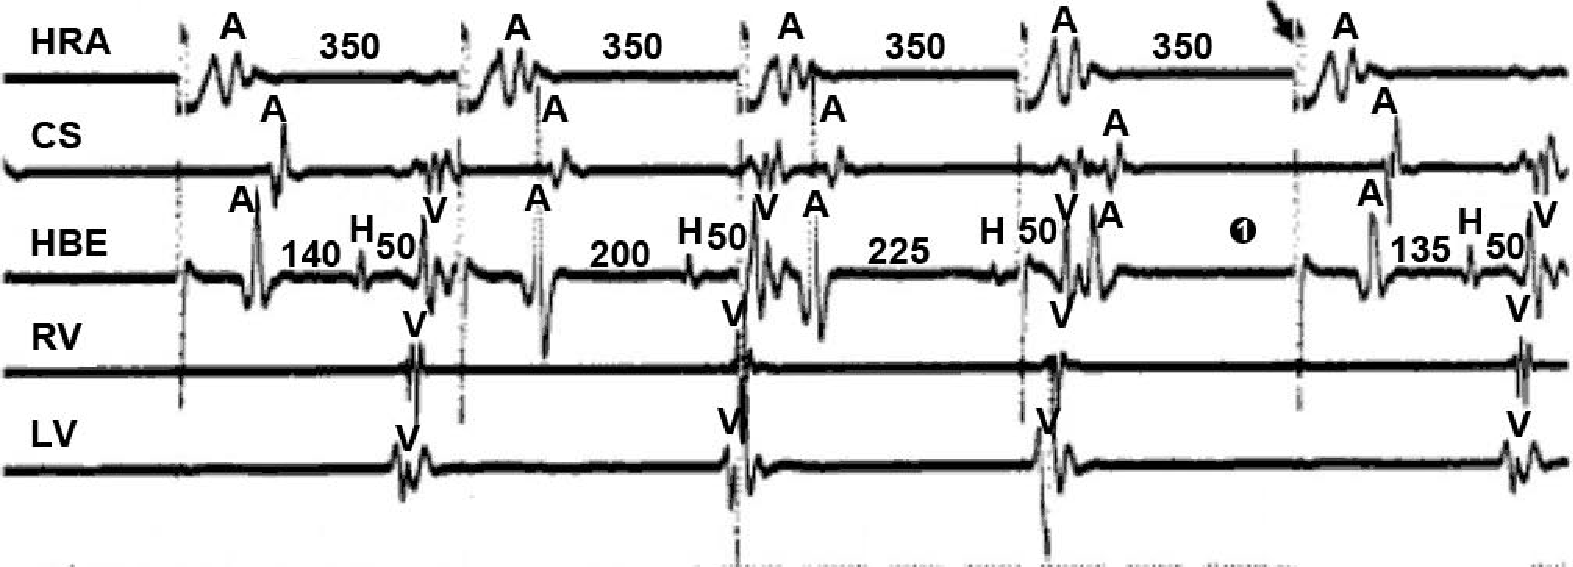
\includegraphics[width=0.7\textwidth]{figs/wenckebach_book.pdf}
		\label{fig:WB_book}
		} 
		\hspace{.1in}%
		\subfigure [\small Heart model's electrograms] 
		{	
			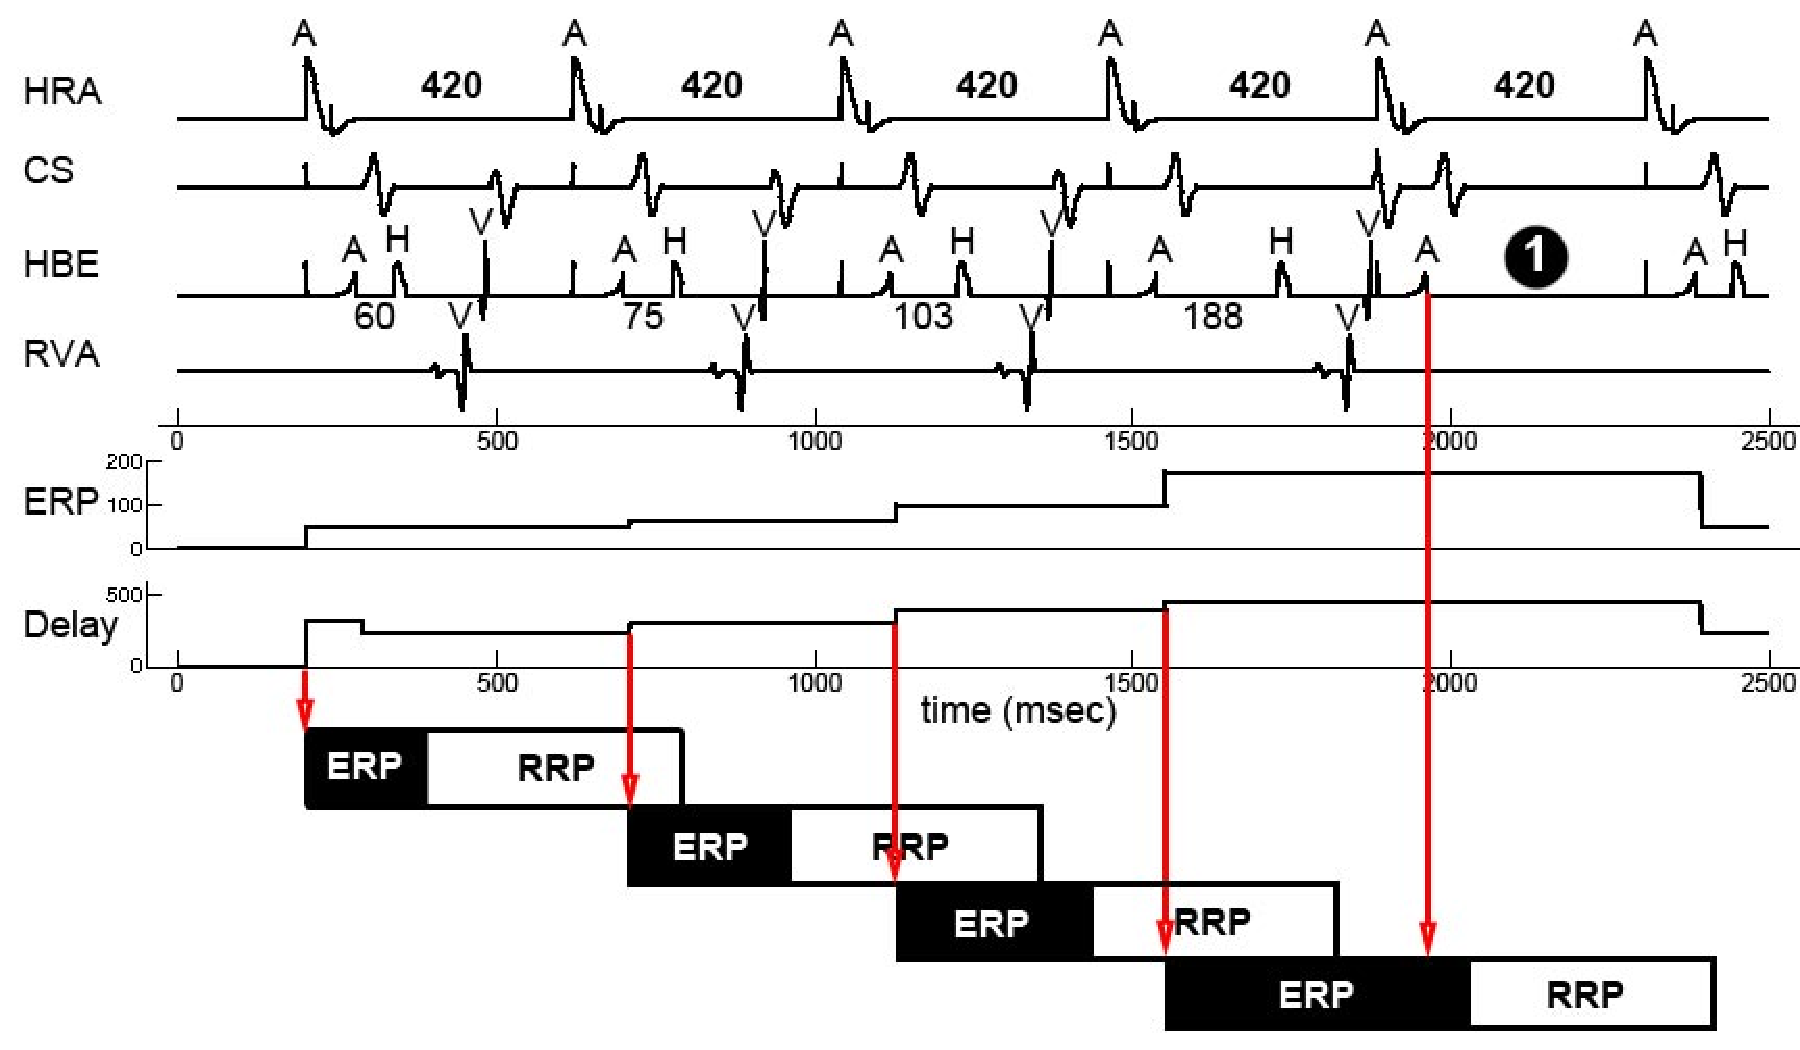
\includegraphics[width=0.7\textwidth]{figs/WB_new.pdf} 
			\label{fig:WB}
		}
\caption{(a) Electrograms of induced Wenckebach block in a patient. (b) Electrograms of induced Wenckebach block in the heart model with a basic cycle length of 420 msec. The heart model also displays lengthening in the A-H interval and block in A-V node (Marker 1). Rows 5 and 6 show the increase in the ERP and conduction delay of the A-V node.}
\end{figure*} 
%%%%%%%%%%%%%%%%%%%%%%%%%%%%%%%%%%%%%%%%%%%%

\noindent\textbf{Validation by comparison to real patients:} This heart condition can also show Wenckebach type A-V nodal response. In this case, a sequence of pacing signals with a short coupling interval ($A_1-A_2<=AV.Terp+AV.Trrp$) is delivered in the atrium. This results in a gradual increase in the AV nodal conduction delay and then a dropped beat occurs in the ventricle due to the increased ERP period of the AV node. The EGMs for a real patient with Wenckebach type A-V nodal response are shown in \figref{WB_book}. With the VHM, we observe similar behavior, and the gradually increasing ERP and conduction delay are visualized in \figref{WB}.
\subsection{Validating Models for Closed-loop Model Checking}
In model checking, a lot of complex dynamics of the environment are abstracted so that the environment model covers a larger number of environmental behaviors using non-determinism. The validity of the model is obtained by a valid initial model and a rigorous abstraction processes. In \cite{STTT13}, we started with a valid detailed deterministic model (as described above) and by applying different abstraction steps we were able to generate a series of non-deterministic heart models. Between each abstraction step, the heart models satisfy a timed simulation relationship (\cite{simulation}) which is described below. The timed simulation guarantees all behaviors are covered in the more abstract model.
More details regarding heart model abstraction will be discussed in Chapter 3.

\section{EP Heart Model Identification}

Physiological models are developed to represent certain clinical conditions common across a population of patients, or the conditions of a specific patient. 
Consequently, the structure of the model and corresponding parameters have to be identified. 
This information can be obtained from electrogram data collected during medical procedures and from physiological literature in which population data has been analyzed and summarized. 
Due to limited interactions with the patient (e.g. during a device implantation procedure or an ablation procedure), currently the quality and quantity of patient-specific physiological data is sparse as there is generally not enough information to identify all the parameters in the heart model.  
A model with the spatio-temporal structure that is similar to the conduction patterns in the heart helps simplify the process of identifying the model parameters. 
A rigorous procedure for the model identification step is an important contributor to the model validation step. 
%%It is essential to choose the right level of abstraction so that the model is identifiable (to a large extent). Having physiological correspondence for the model structure and parameters can also simplify the identification process. 
\begin{figure}[t]
\center
	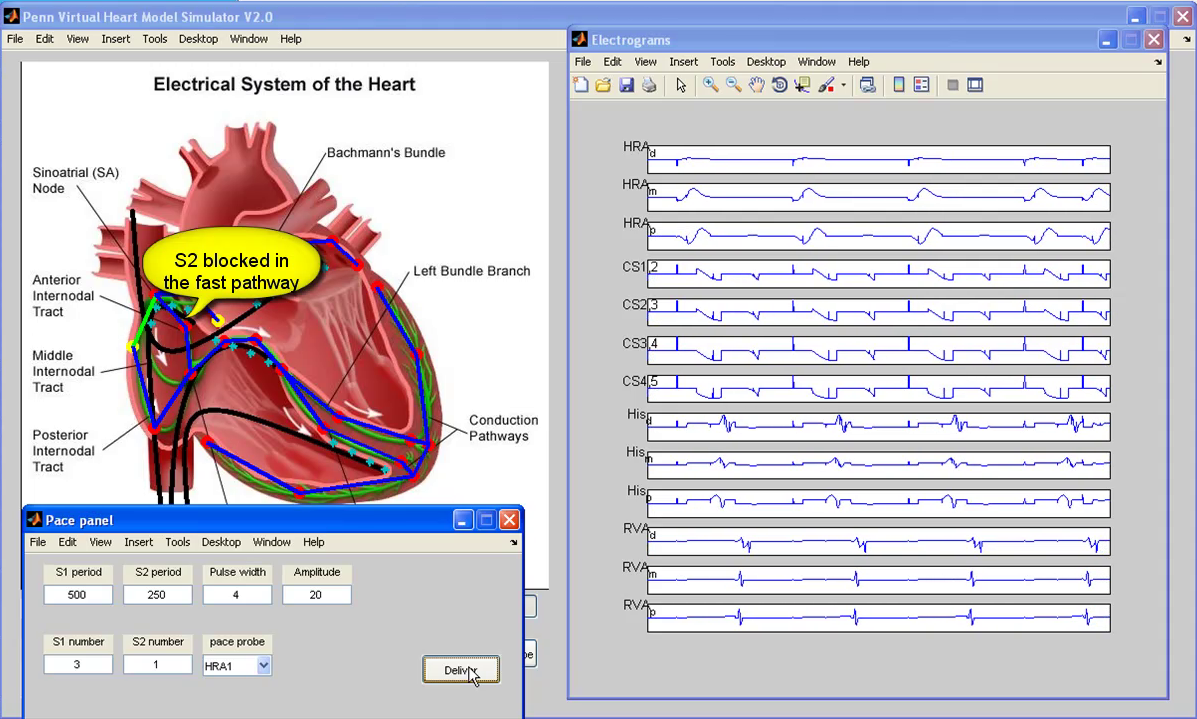
\includegraphics[width=0.9\textwidth]{figs/vhmsim.png}
	\caption{Simulation model of the heart showing the conduction pathways (left) with electrogram signals from different probe locations (right) and an interactive pacing panel (bottom left). In this case, the heart was paced four times at an interval of 500ms, followed by a pacing at a shorter (250ms) interval. This EP Testing procedure is employed to trigger conduction along alternative pathways and check for the existence of a reentry circuit.}
	\label{fig:vhmsim}
\end{figure}
In this section, we briefly discuss our model identification effort for heart models used in two closed-loop validation applications, and their corresponding challenges. 

\begin{figure}[!b]
\centering
		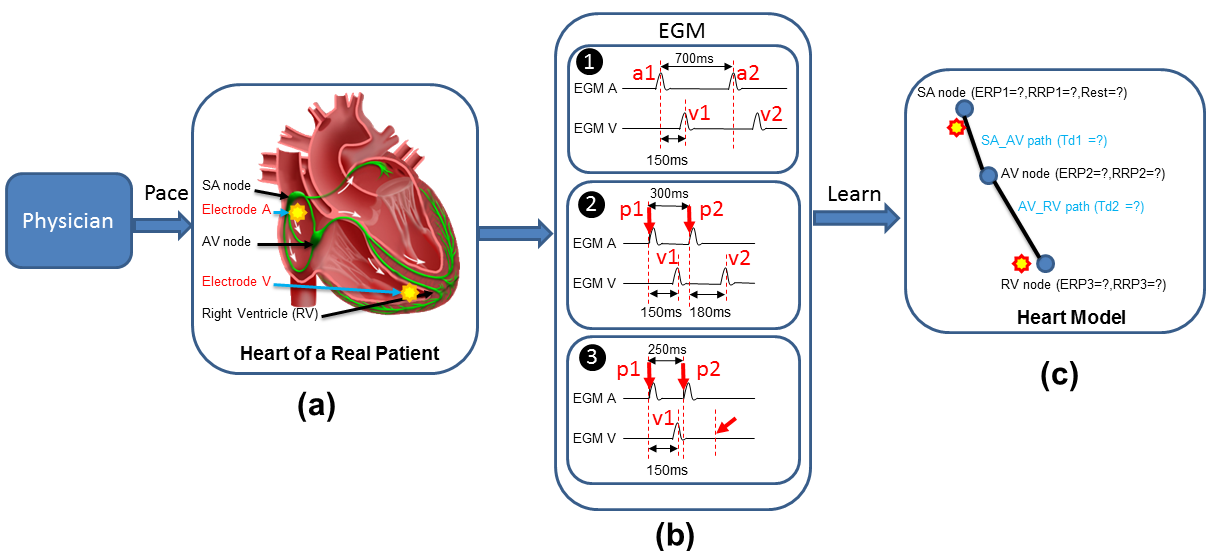
\includegraphics[width=0.9  \textwidth]{figs/modelID.png}
		
%\vspace{-10pt}
\caption{\small (a) The illustration of the probe locations. (b) Multiple pacing sequences with different timing outcomes. (c) The heart model with undecided parameters}
\label{fig:modelID}
%\vspace{-15pt}
\end{figure} 

\subsection{Heart Model Identification for Closed-loop Testing}
In closed-loop simulation, a deterministic heart model should be identified to represent a specific patient under a certain heart condition. The constraints for model parameters can be obtained from patient data with \emph{Electrophysiological (EP) Testing}. During EP testing, the physician delivers electrical pacing sequences from electrodes placed inside the patient's heart to instigate responses along fast and slow conduction pathways (\figref{vhmsim}). The observed patterns and timing of electrical events are used to extract conduction and propagation properties of different tissue regions across the myocardium. Since the goal for any EP testing procedure is not to determine all the timing parameters for a patient, the number of parameters that can be identified from the patient data is limited.    

\figref{modelID} illustrates how timing parameters can be extracted during an EP testing procedure. \figref{modelID}(a) shows a setup with two electrodes placed in the right atrium and right ventricle of the heart respectively. EGM signals can be measured from these two electrodes (\figref{modelID}(b)). The physician delivers a series of long interval pacing sequences followed by one or more short interval pacing through the electrodes. This may trigger different responses along primary and alternate conduction pathways from the patient's heart. \figref{modelID}(c) shows a heart model structure with unknown parameter values. By analyzing the \emph{timing} and \emph{pattern} of the EGM signals we extract constraints on the heart model parameters. In EGM sequence 1, the interval between two intrinsic activations $a1$ and $a2$ in EGM A is 700ms, so we have:
$$ERP1+RRP1+Rest=700ms$$
The interval between $a1$ and $v1$ is 150ms, so we have:
$$Td1+Td2=150ms$$
In EGM sequence 2, the pacing interval from Electrode A is 300ms. By observing that the interval between $p1-v1$ is less than the interval between $p2-v2$, we know that $p2$ arrives during the RRP period of the AV node. So we have:
$$ERP1+RRP1\leq 300ms$$
In EGM sequence 3, the pacing interval is further reduced to 250ms. There is no $v2$ corresponding to $p2$, indicating $p2$ arrives during the ERP period of the AV node. So we have:
$$ERP1\leq 250ms$$
Each experiment provides additional time constraints for model parameters. By systematically conducting experiments certain model parameters can be uniquely identified within a relatively tight range. However, even with simplified model structure like the one in the example, not all model parameters can be uniquely identified due to limited number of electrodes and limited number of experiments during a real procedure.






\subsubsection{Heart Model Identification in Closed-loop Model Checking}
In model checking, the heart models have simpler structure and fewer parameters due to non-deterministic abstraction. The placement and connectivity of nodes and paths in the heart models are developed to be consistent with EP practice. This way, each node and path automata and their timing parameters have physiological correspondence to parameters found in literature (\figref{intervals}). The range for non-deterministic parameters directly corresponds to the range for possible values of the respective physiological parameters. Therefore, model identification for model checking is much simpler and requires less EP testing data. It is important to note here that model checking of abstract models of the closed-loop system and testing of the device in the loop are complementary approaches for validating the safety and efficacy of the overall system. 

\begin{figure}[!t]
\centering
		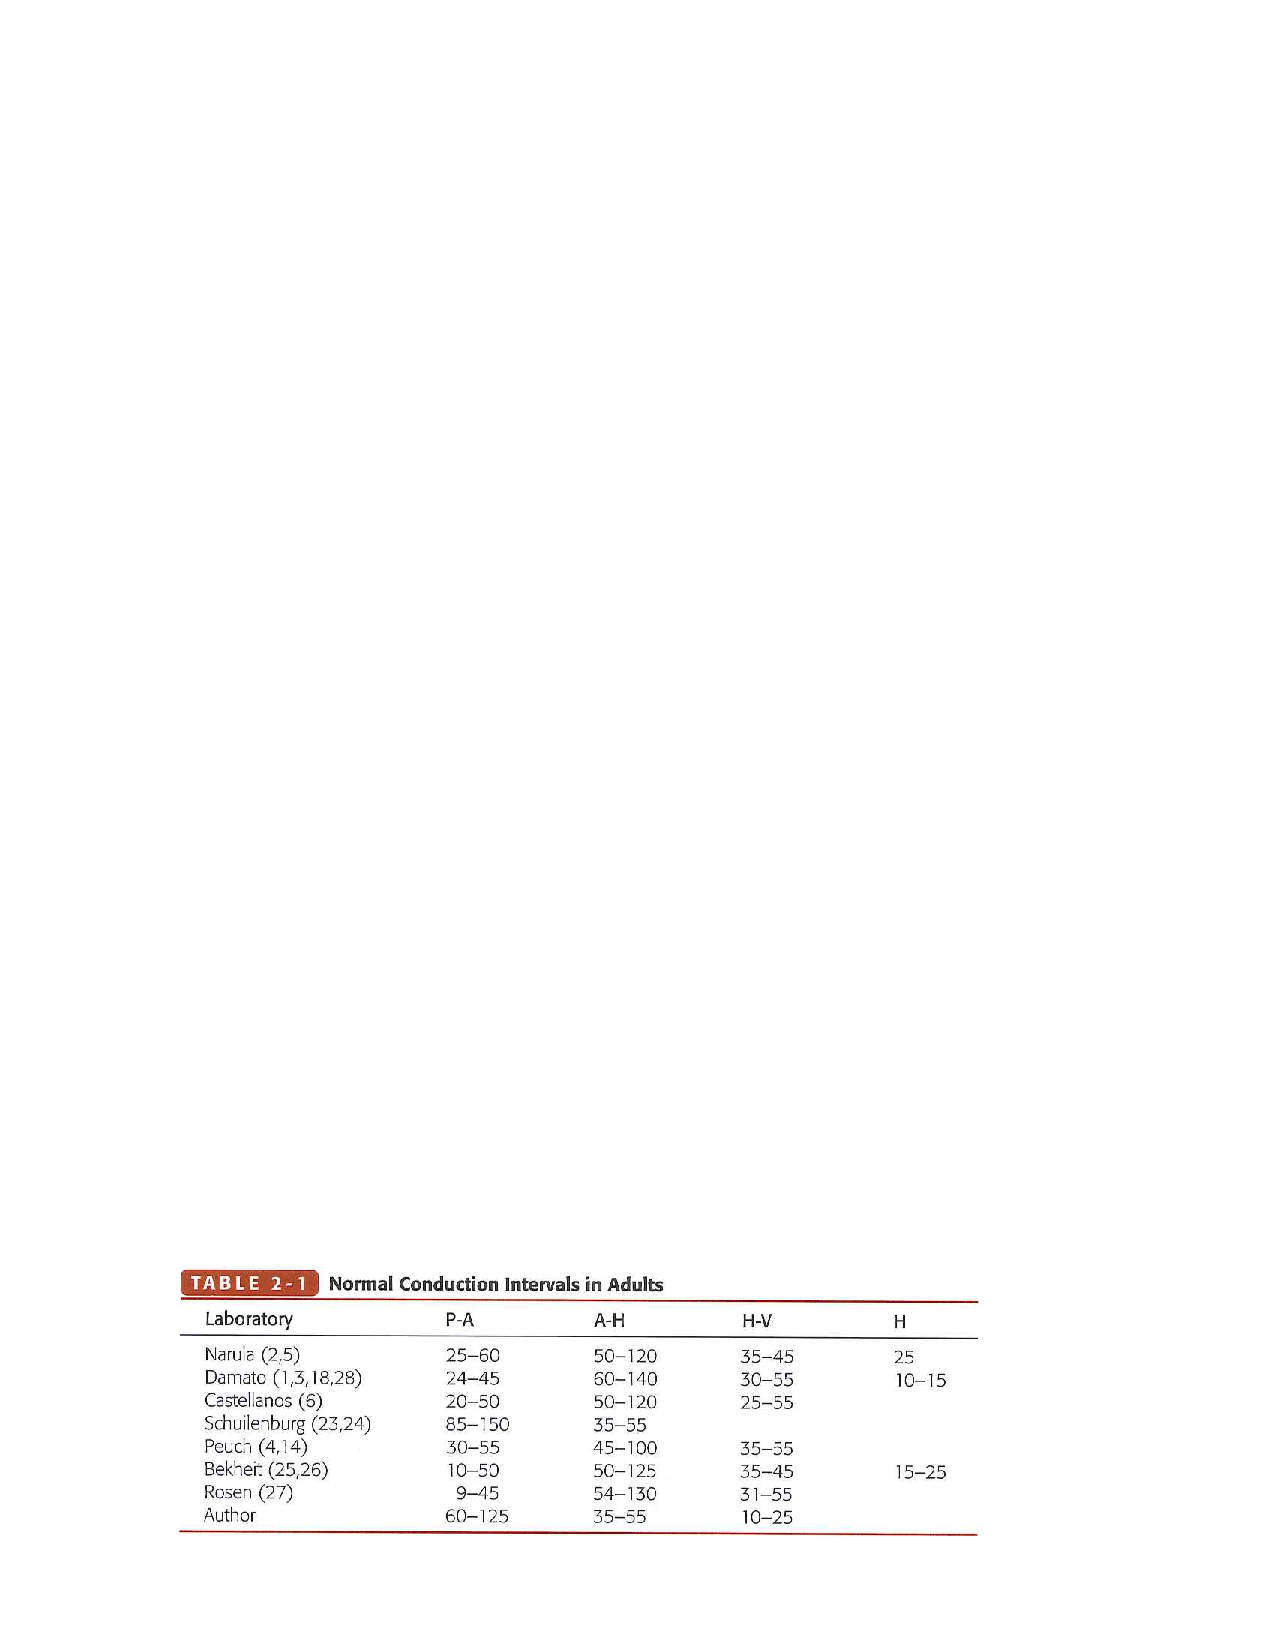
\includegraphics[width=0.8\textwidth]{figs/intervals.pdf}
		
%\vspace{-10pt}
\caption{\small Timing intervals measured during clinical studies \cite{josephson}}
\label{fig:intervals}
%\vspace{-15pt}
\end{figure} 



%%%%%%%%%%%%%%%%%%%%%%%%%%%%%%%%%%%%%
%%%%%%%%%%%%%%%%%%%%%%%%%%%%%%%%%%%%%




\section{Discussion}
%Physiological modeling is the most important aspect for closed-loop validation of autonomous medical devices.
The quality and validity of closed-loop validation results depend on the quality and validity of the physiological models.
It is essential for the physiological models to be complex enough to accurately interpret the behaviors of physiological conditions, and abstract enough to be identifiable from patient data.
In this chapter, an EP heart model structure is developed for closed-loop evaluation of implantable cardiac devices. 
The heart model structure is capable of representing different heart conditions and its parameters can be identified from patient data.
In the remaining dissertation, the heart model structure will be used in different model-based techniques to provide safety and efficacy evidence for implantable cardiac devices.



 
\chapter{A Dual Chamber Pacemaker Specification}

As part of the model-based design, it is important to have a functional and formal model of the device software for testing and formal verification respectively. In our study, we focus on the implantable  pacemaker since it is one of the simpler implantable cardiac devices as its functionality is based only on timing and does not consider signal morphology. This serves as a good base case to demonstrate the proposed methodology.  In this chapter, we describe the basic specification and formal implementation of a dual chamber pacemaker, as well as a more advanced function on mode switching. The specifications are based on the algorithm descriptions from Boston Scientific manuals (\cite{compass}) and the functional description released as part of the Pacemaker Challenge (\cite{challenge}). 
We aim to answer the following questions here:
\begin{itemize}
	\vspace{-5pt}
	\item How are the pacemaker's timers specified to maintain the appropriate heart rhythm?
	\vspace{-5pt}
   	\item What happens if new functionality is added to the basic model?
\end{itemize}

The artificial pacemaker is designed for patients with bradycardia (i.e. slow heart rate). Two leads, one in the right atrium and one in the right ventricle, are inserted into the heart and fixed onto the inner wall of the heart. These two leads monitors the local activation of the atria and the ventricles, and generate corresponding sensed events \textsf{(AS, VS)} to its software. The software determines the heart condition by measuring time difference between events and delivers pacing events \textsf{(AP, VP)} to the analog circuit when necessary. The analog circuit then delivers pacing signals to the heart to maintain heart rate and A-V synchrony. In order to deal with different heart condition, pacemakers are able to operate in different modes. The modes are labeled using a three character system (e.g. $xyz$). The first position describes the pacing locations, the second location describes the sensing locations, and the third position describes how the pacemaker software responds to sensing. Here we introduce the widely used DDD mode pacemaker which is a dual chamber mode with sensing and pacing in both atrium and ventricle. 

\begin{figure}[!b]
\center
%\vspace{-10pt}
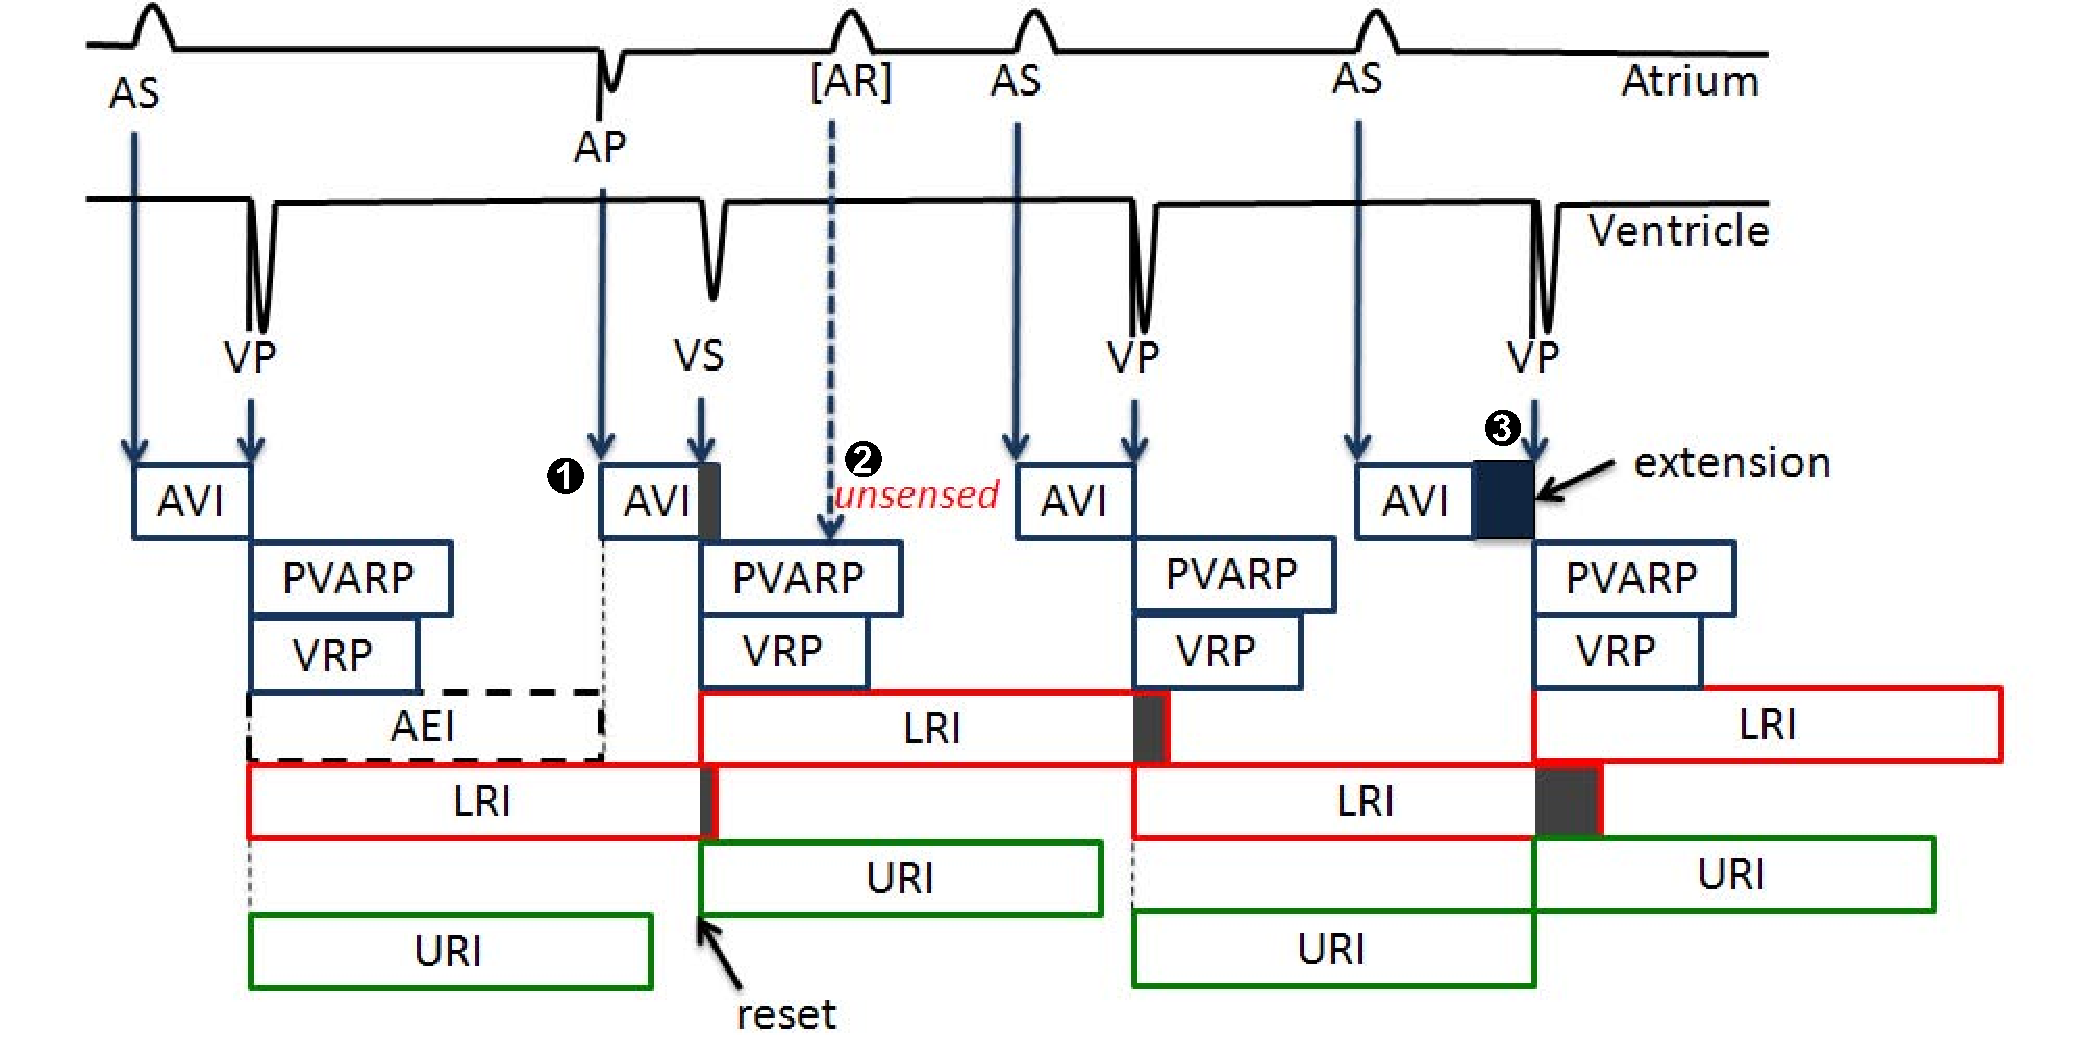
\includegraphics[width=0.85\textwidth]{figs/PM_timers.pdf}
%\vspace{-10pt}
\caption{Basic 5 timing cycles for a dual chamber pacemaker which include the Lower Rate Interval (LRI),  Atrio-Ventricular Interval (AVI), and Upper Rate Interval (URI). Also included are the blanking intervals, Post Ventricular Atrial Refractory Period (PVARP) and Ventricular Refractory Period (VRP), to inhabit action by the pacemaker.}
\label{fig:PMtimers}
%\vspace{-10pt}t

\end{figure} 
\section{Basic Specifications of a DDD Pacemaker}
The DDD pacemaker has five basic timing cycles triggered by external and internal events, as shown in \figref{PMtimers}. We decomposed our pacemaker model into five components which correspond to the five timers. $P=LRI\| AVI\| URI\| PVARP\| VRP$. These components synchronize with each other using broadcast channels and shared variables (as shown in \figref{PMdesign}). 

\subsection{Lower Rate Interval (LRI)}
%\vspace{-5pt}
The Lower Rate Interval (LRI) component is shown in \figref{PMdesign}(a). This component defines the longest interval allowed between two ventricular events, thus keeping the heart rate above a minimum value. In DDD mode, the LRI interval is divided into a V-A interval (TLRI-TAVI) and a A-V interval (TAVI). The LRI component maintains a maximum V-A delay while the AVI component maintains a maximum A-V delay so together they maintain the maximum V-V delay. In the LRI component, the clock is reset when a ventricular event \textsf{(VS, VP)} is received. If no atrial event has been sensed \textsf{(AS)}, the component will deliver atrial pacing \textsf{(AP)} after TLRI-TAVI. 

%\vspace{-5pt}
\subsection{Atrio-Ventricular Interval (AVI) and Upper Rate Interval (URI)}
%\vspace{-5pt}
The function of the AVI component defines the longest interval between an atrial event and a ventricular event. If there is no ventricular event \textsf{(VS)}  within TAVI after an atrial event \textsf{(AS, AP)}, and the time since the last ventricular event \textsf{(VS, VP)} is longer than TURI, the component will deliver ventricular pacing \textsf{(VP)}. The URI limits the ventricular pacing rate by enforcing a lower bound on the times between consecutive ventricle events. The UPPAAL design of AVI and URI component is shown in \figref{PMdesign}(b) and (c).%The UPPAAL design of AVI component is shown in 

%\vspace{-10pt}
\subsection{Post Ventricular Atrial Refractory Period (PVARP) and Post Ventricular Atrial Blanking (PVAB)}
%\vspace{-5pt}
Ventricular events, especially Ventricular Pace \textsf{(VP)} are sometimes so strong that the atrial lead can sense the activation as well. This signal may be falsely recognized as an atrial event and disrupt normal pacemaker function. This scenario is called crosstalk and was discussed in our previous work (\cite{vhm_embc11}). In order to prevent this undesired behavior, and filter potential noises, there is a blanking period (PVAB) followed by a refractory period (PVARP) for the atrial events after each ventricular event \textsf{(VS, VP)}. Atrial events during PVAB are ignored and atrial events during PVARP trigger \textsf{AR!} events which can be used in some advanced diagnostic algorithms. The UPPAAL design of PVARP component is shown in \figref{PMdesign}(d).

%\vspace{-10pt}
\subsection{Ventricular Refractory Period (VRP)}
%\vspace{-5pt}
The VRP follows each ventricular event \textsf{(VP, VS)} to filter noise and early events in the ventricular channel which could otherwise cause undesired pacemaker behavior. \figref{PMdesign}(e) shows the UPPAAL design of VRP component.

\begin{figure}[!t]
\center
%\vspace{-10pt}
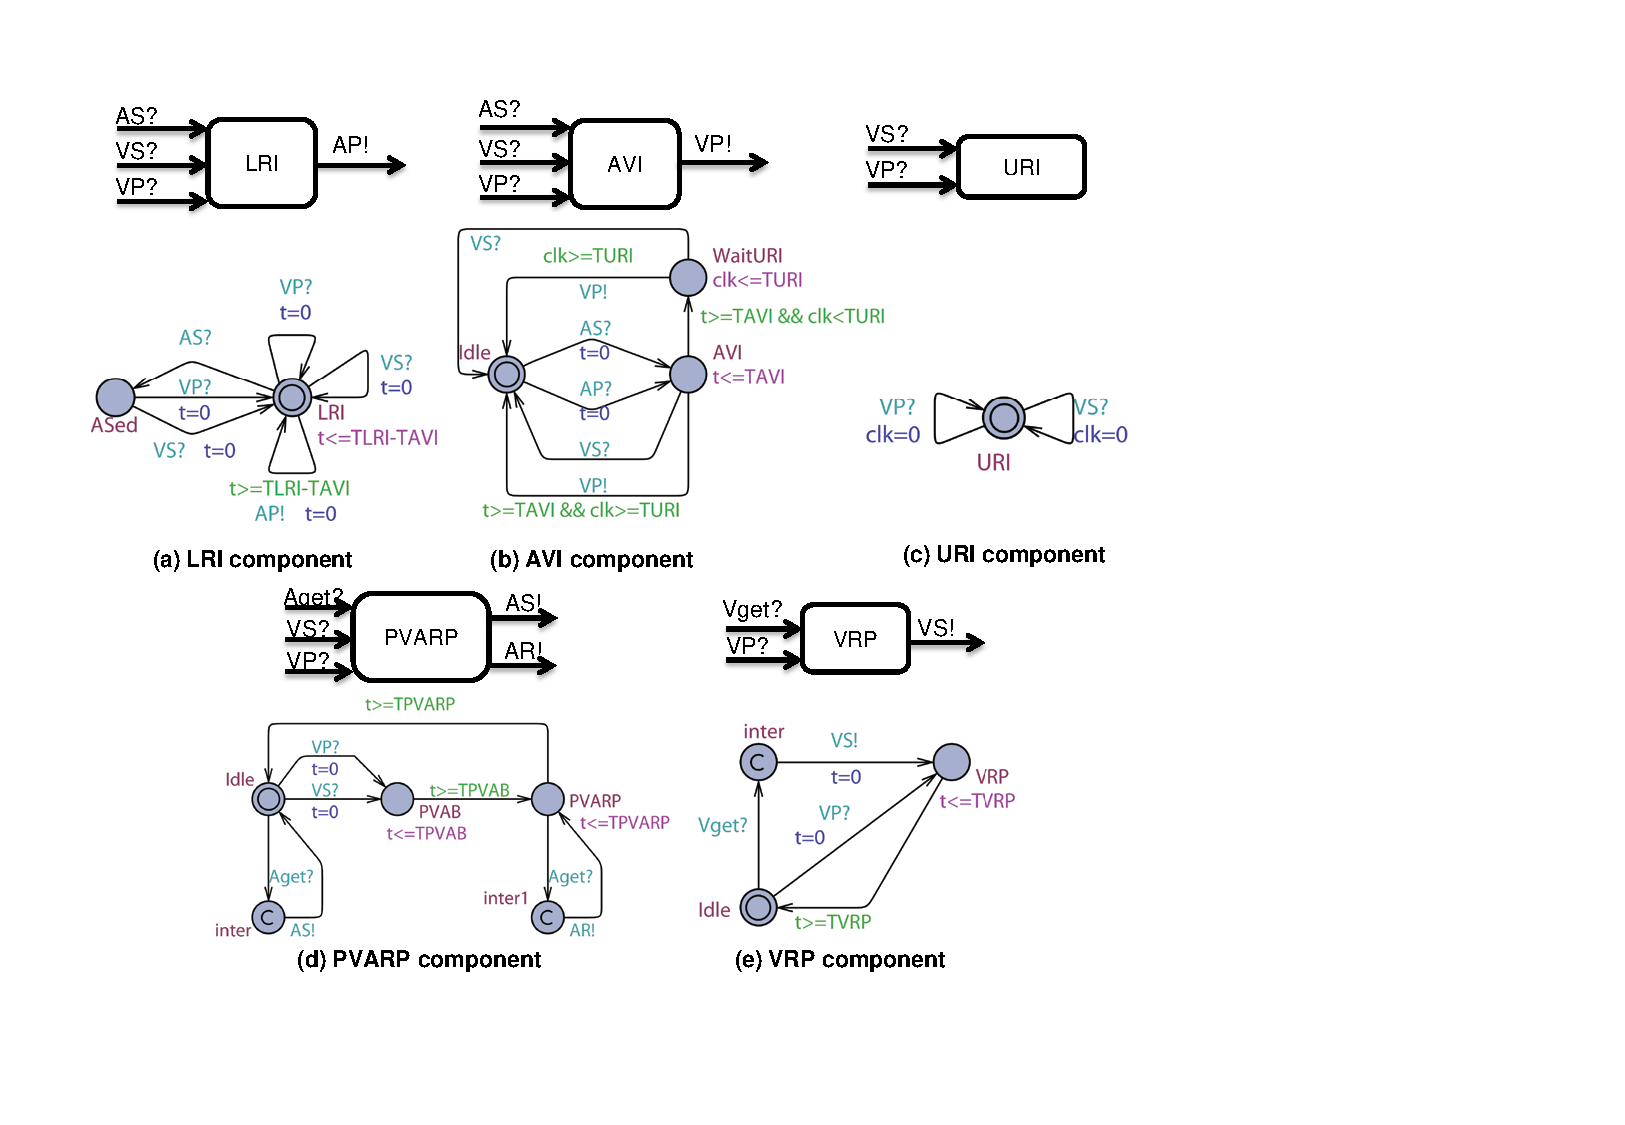
\includegraphics[width=0.9\textwidth]{figs/pacemaker.pdf}
%\vspace{-10pt}
\caption{Five basic timing cycles for a dual chamber pacemaker, which include the Lower Rate Interval (LRI), Atrio-Ventricular Interval (AVI), and Upper Rate Interval (URI). Also included are the blanking intervals, Post Ventricular Atrial Refractory Period (PVARP) and Ventricular Refractory Period (VRP), to inhabit action by the pacemaker.}
\label{fig:PMdesign}
%\vspace{-10pt}
\end{figure} 

\section{Mode Switch Operation: Atrial Tachycardia Response}
\label{Mode_switch}
Supraventricular Tachycardia (SVT) is an arrhythmia with an abnormally fast atrial rate. %\figref{SVT} is a series of simulation results for closed-loop interaction between a heart model with SVT and the pacemaker model. The atrial and ventricular channels show electrogram inputs to the pacemaker and the pacemaker channel shows the corresponding events received and generated by the pacemaker software, \cite{vhm_embc11}.
Typically, in a heart without pacemaker, the AV node, which has a long refractory period, can filter most of the fast atrial activations during SVT, thus the ventricular rate remains relatively normal. \figref{SVT_none} demonstrates a pacemaker event trace during SVT, with a pacemaker in ODO mode, which just sensing in both channels. 
As there is no pacing in ODO mode, the heart is in open-loop with the pacemaker. In this particular case, every 3 atrial events (AS) correspond to 1 ventricular event (VS) during SVT. 
As an arrhythmia, SVT is still considered a safe heart condition since the ventricles operate under normal rate and still maintain adequate cardiac output. 

However, in the closed loop case with the DDD pacemaker, the AVI component of a dual chamber pacemaker is equivalent to a virtual pathway in parallel to the intrinsic conduction pathway between the atria and the ventricles. The pacemaker tries to maintain 1:1 A-V conduction and thus increases the ventricular rate inappropriately to match the atrial rate.  This is known as Pacemaker Mediated Tachycardia (PMT) as the heart would have been safe without the pacemaker and its virtual pathway. \figref{SVT_DDD} shows the pacemaker trace of the same SVT case with DDD pacemaker. Although half of the fast atrial events are filtered by the PVARP period ([AR]s), the DDD pacemaker still drives the closed-loop system into 2:1 A-V conduction with faster ventricular rate. Maintaining A-V delay is less important than maintaining an appropriate ventricular rate. The DDD pacemaker violates a higher priority requirement in order to satisfy a lower priority requirement, which is inappropriate.
\begin{figure*}[!t]
\centering
		\subfigure [\small]{			
		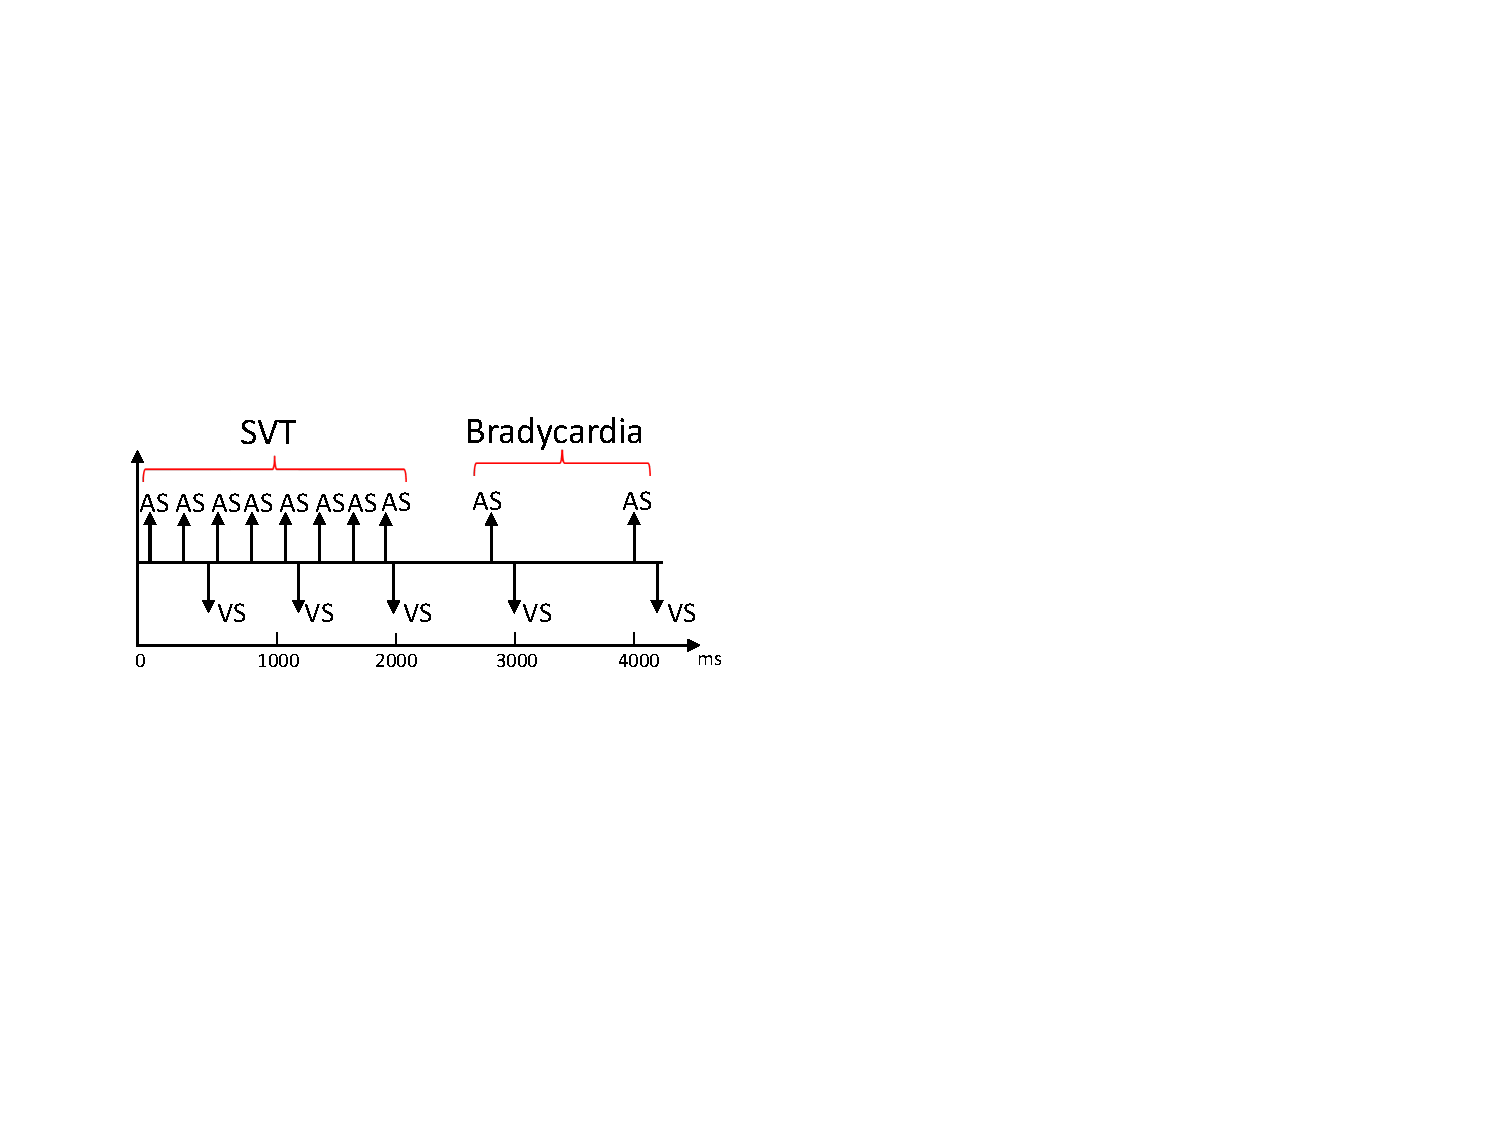
\includegraphics[width=0.5  \textwidth]{figs/SVT_none.pdf}
		\label{fig:SVT_none}
		} 
%	\hspace{.1in}%
\vspace{-10pt}
		
		\subfigure [\small] 
		{
		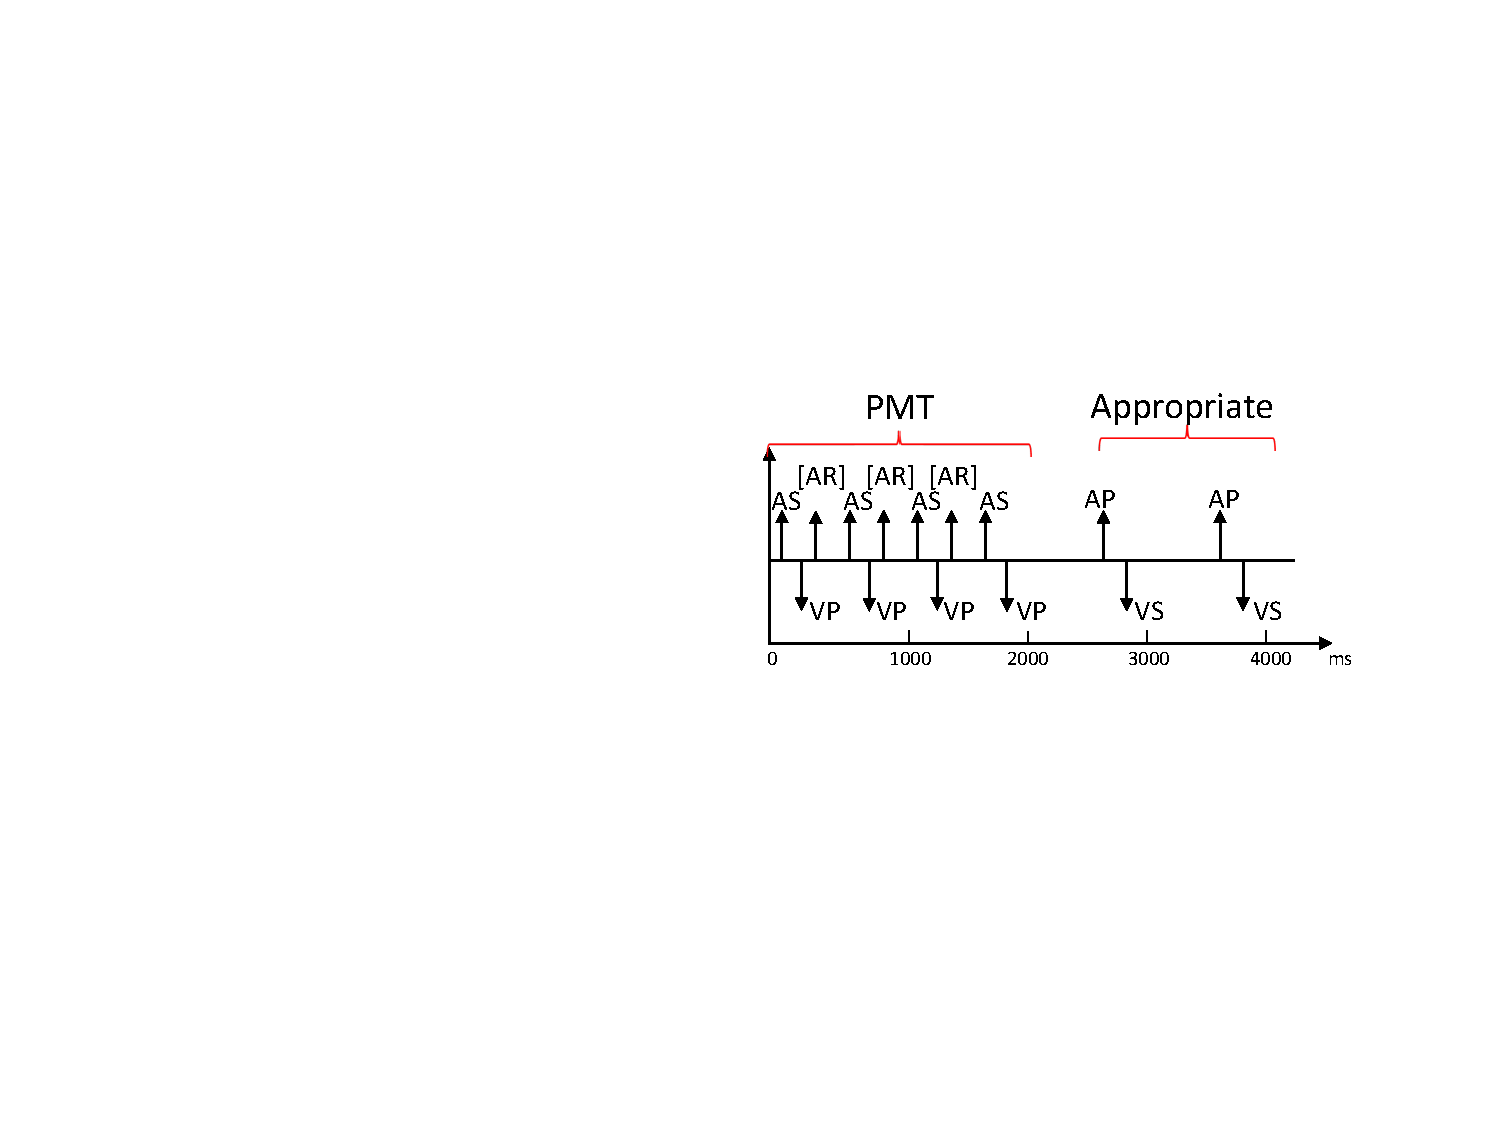
\includegraphics[width=0.5\textwidth]{figs/SVT_DDD.pdf}
		\label{fig:SVT_DDD}
		} 
\vspace{-5pt}
\caption{\small Benign open loop case: SVT without a pacemaker or with a pacemaker in sense-only mode (ODO) (b) Dangerous closed-loop-case SVT with DDD pacemaker which tries to match the fast atrial rate with a corresponding (and dangerous) fast ventricular rate.}
\vspace{-10pt}
\end{figure*} 

Pacemaker manufacturers have designed algorithms to detect and terminate these behaviors. Intuitively, the mode-switch algorithm first detects SVT. After confirmed detection, it switches the pacemaker from a dual-chamber mode to a single-chamber mode. During the single-chamber mode, the A-V synchrony function of the pacemaker is deactivated thus the ventricular rate is decoupled from the fast atrial rate. After the algorithm determines the end of SVT, it will switch the pacemaker back to the dual chamber mode. 
\begin{figure*}
		\centering
		%\vspace{-19pt}
		\includegraphics[width=0.8\textwidth]{figs/AVI_ms.pdf}
		%\vspace{-10pt}
		\caption{\small (a) After switching to \textsf{VDI} mode, the new LRI component \textsf{LRI'} maintains a minimum V-V interval; (b) After switching to \textsf{VDI} mode, the new AVI component \textsf{AVI'} keeps track of the time after each atrial events.}
		%  \vspace{-20pt}
		\label{fig:avi_ms}
\end{figure*}
The mode-switch algorithm (also known as atrial tachycardia response) specification we use is similar to the one described in the Boston Scientific pacemakers' manual (\cite{compass}). The algorithm first measures the interval between atrial events outside the blanking period (AS, AR). The interval is considered as \emph{fast} if it is above a threshold (\emph{Trigger Rate}) and \emph{slow} otherwise. In our UPPAAL model we model it as $INT$ (see \figref{dur_count} (1)). A counter $CNT$ increments for \emph{fast} events and decrements for \emph{slow} events (see \figref{dur_count} (2)). After the counter value reaches the \emph{Entry Count}, the algorithm will start a \emph{Duration} ($DUR$) ,which is a time interval used to confirm the detection of SVT (see \figref{dur_count} (3)). In the \emph{Duration}, the counter keeps counting. If the counter value is still positive after the \emph{Duration}, the pacemaker will switch to the VDI mode (\emph{Fallback mode}). In the VDI mode, the pacemaker only senses and paces the ventricle. At any time if the counter reaches zero, the \emph{Duration} will terminate and the pacemaker is switched back to DDD mode.
% to show some interesting findings. The basic idea of this simplified model is explained in detail. \\
%\mySubSubSection{UPPAAL model for mode-switch algorithm}
In our UPPAAL model of the mode-switch algorithm, we use nominal parameter values from the clinical setting. We define \emph{trigger rate} at 170bpm (350ms), \emph{entry count} at 8, \emph{duration} for 8 ventricular events and \emph{fallback mode} as VDI. 
\begin{figure*}
		\centering
				%\vspace{-15pt}
		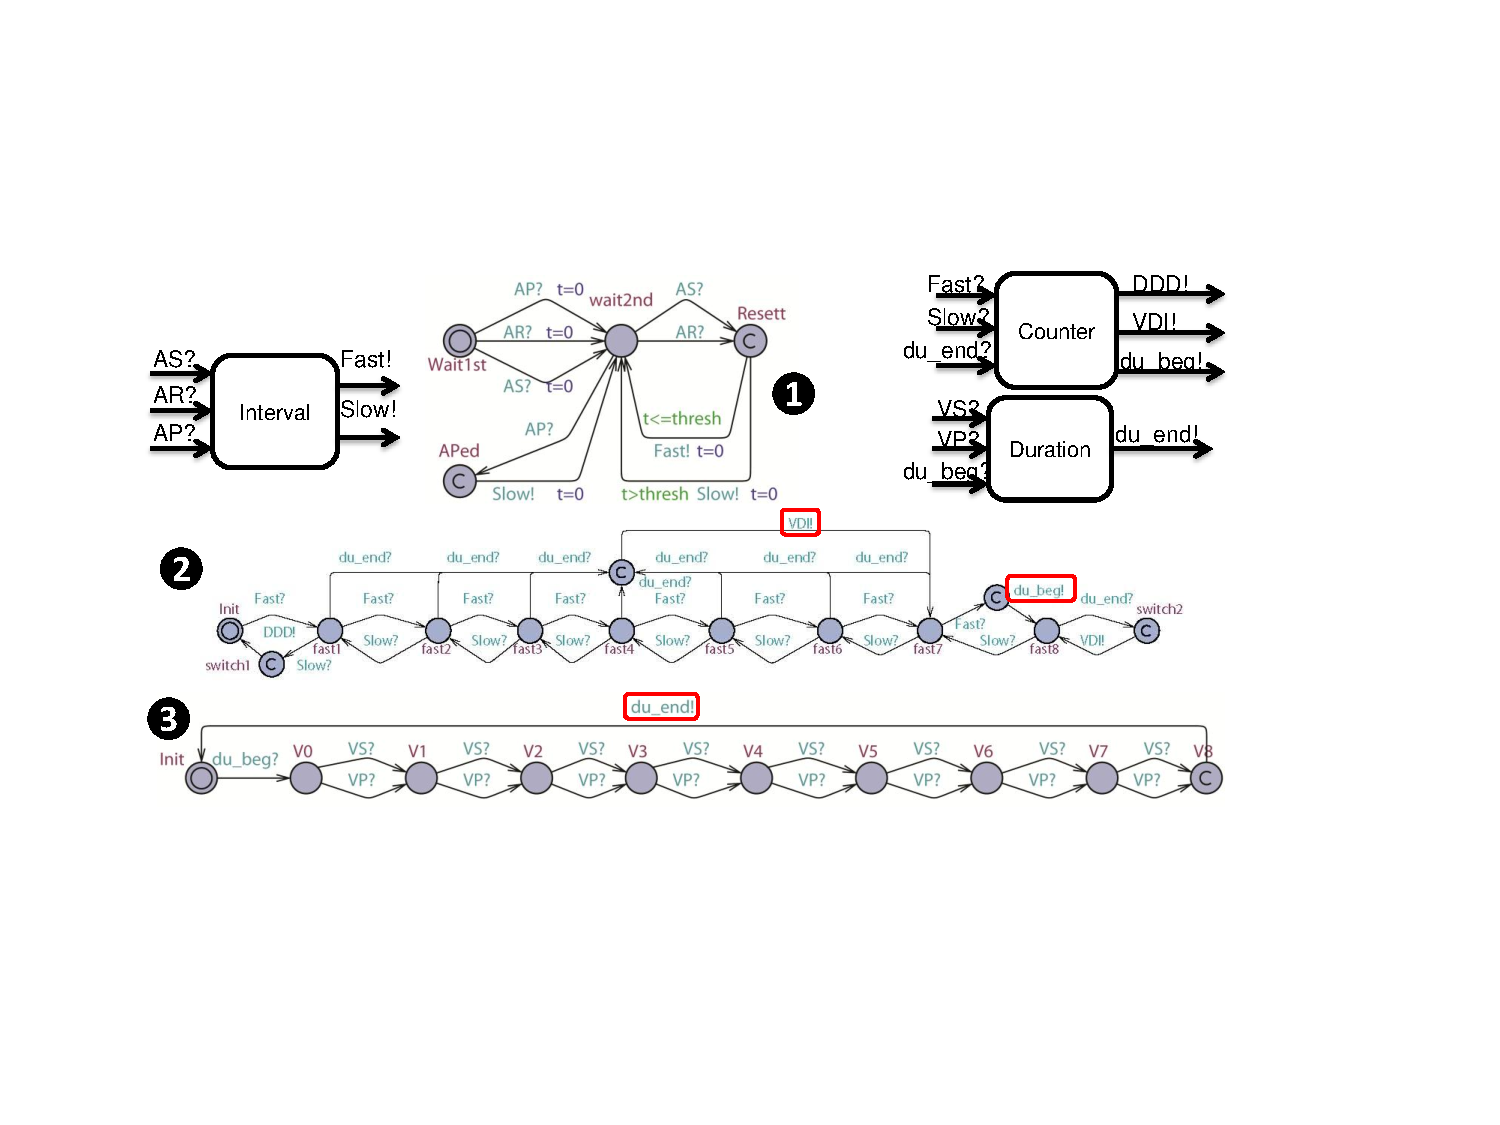
\includegraphics[width=0.9\textwidth]{figs/duration.pdf}
		%\vspace{-10pt}
		\caption{\small (1) Component \textsf{INT}: An atrial event (\textsf{AS,AR}) arrives before \textsf{thresh} after the previous atrial event is regarded as a \textsf{fast} event. Atrial event arrives after \textsf{thresh} and \textsf{AP} are regarded as \textsf{slow} event; (2) Component \textsf{CNT}: After 8 \textsf{fast} event the algorithm will start a duration by sending \textsf{du\_beg} and will switch to \textsf{VDI} mode when the duration ends (\textsf{du\_end}); (3) Component \textsf{DUR} :The duration length is 8 ventricular events (\textsf{VS,VP})}
		  %\vspace{-15pt}
		\label{fig:dur_count}
\end{figure*} 

In order to model both DDD and VDI modes and the switching between them, we made modifications to the AVI and LRI components.
In each component two copies for both modes are modeled, and switch between each other when switching events (DDD, VDI) are received. During VDI mode, \textsf{VP} is delivered by the LRI component instead of the AVI component. The clock values are shared between both copies in order to preserve essential intervals even after switching. The modified AVI ($AVI'$) and LRI ($LRI'$)components are shown in \figref{avi_ms}. 
\looseness-1


%%%%%%%%%%%%%%%%%%%%%%%%%%%%%%%%%%%%%%%%%%%%
%%%%%%%%%%%%%%%%%%%%%%%%%%%%%%%%%%%%%%%%%%%%

\chapter{Closed-loop Model Checking}
\label{ModelChecking}
%There are two categories of device bugs: 
%1) the device may fail to conform to its \emph{specifications}, that is, the prescription of how it should react to certain inputs.  
%2) the device may fail to improve the conditions of the patient as promised, even if it conforms to its specifications. 
%The desired physiological conditions that the closed-loop system should achieve are captured in the \emph{physiological requirements}; for example, for a pacemaker, the heart rate should always be maintained above a certain threshold. 
%
%Bugs in the first category (non-conformance to specification) can be detected via systematic and extensive open-loop testing in which a set of input sequences is fed to the device, and its output is compared with the expected output.
%Bugs in the second category (violation of physiological requirements), on the other hand, require the interaction within the \emph{closed-loop system}, which consists of the device and its environment.
%For instance, the pacemaker and the heart as its environment. 
%In the medical device industry, closed-loop verification of the physiological requirements is mostly performed in terms of clinical trials, in which the actual devices are implanted in human subjects over an extended duration.
%Unfortunately, because of the extremely high cost of clinical trials (several million dollars and spanning several years,~\cite{trialcost}), the amount and variety of human subjects during the clinical trials are limited, which reduces the opportunity to find bugs. 
%Moreover, clinical trials are often conducted at the final design stage. Fixing bugs at this stage is very costly.

Model checking is a technique in which the state space of the model under investigation is automatically and exhaustively explored to identify executions or states that violate specified properties. Violations of the properties are returned by the model checkers as \emph{counter-examples}, which can be used by designers to revise the design. In the application of verification of properties in medical devices like implantable pacemaker, model checking can be used to identify known and unknown mechanisms for inducing hazards. This is extended to checking the heart-pacemaker closed-loop models against physiological hazards (e.g. when the pacemaker provides inappropriate therapy which drives the heart to an unsafe state). 

Due to the curse of dimensionality as models get more complex, and hence the large computational cost, there are usually restrictions on the formalism and the complexity of the models under investigation. Using abstract models of the actual system adds the responsibility of proving the conformance between the abstract model and the real system. Assumptions made during abstractions may also introduce false-positives and/or false-negatives into the model checking results. Back in Chapter 2, we introduced a set of heart models with different abstraction levels, that can be used to cover behaviors of physiological conditions using non-determinism. In Chapter 4, we then modeled a dual chamber pacemaker algorithm using timed-automata without doing abstractions. In this chapter, we use model checker UPPAAL to evaluate the pacemaker model against safety properties under different heart conditions captured by the heart models. Techniques to eliminate false-positives by refining the heart models are also discussed. We will try to answer the following questions:
\begin{figure}[!t]
		\centering
		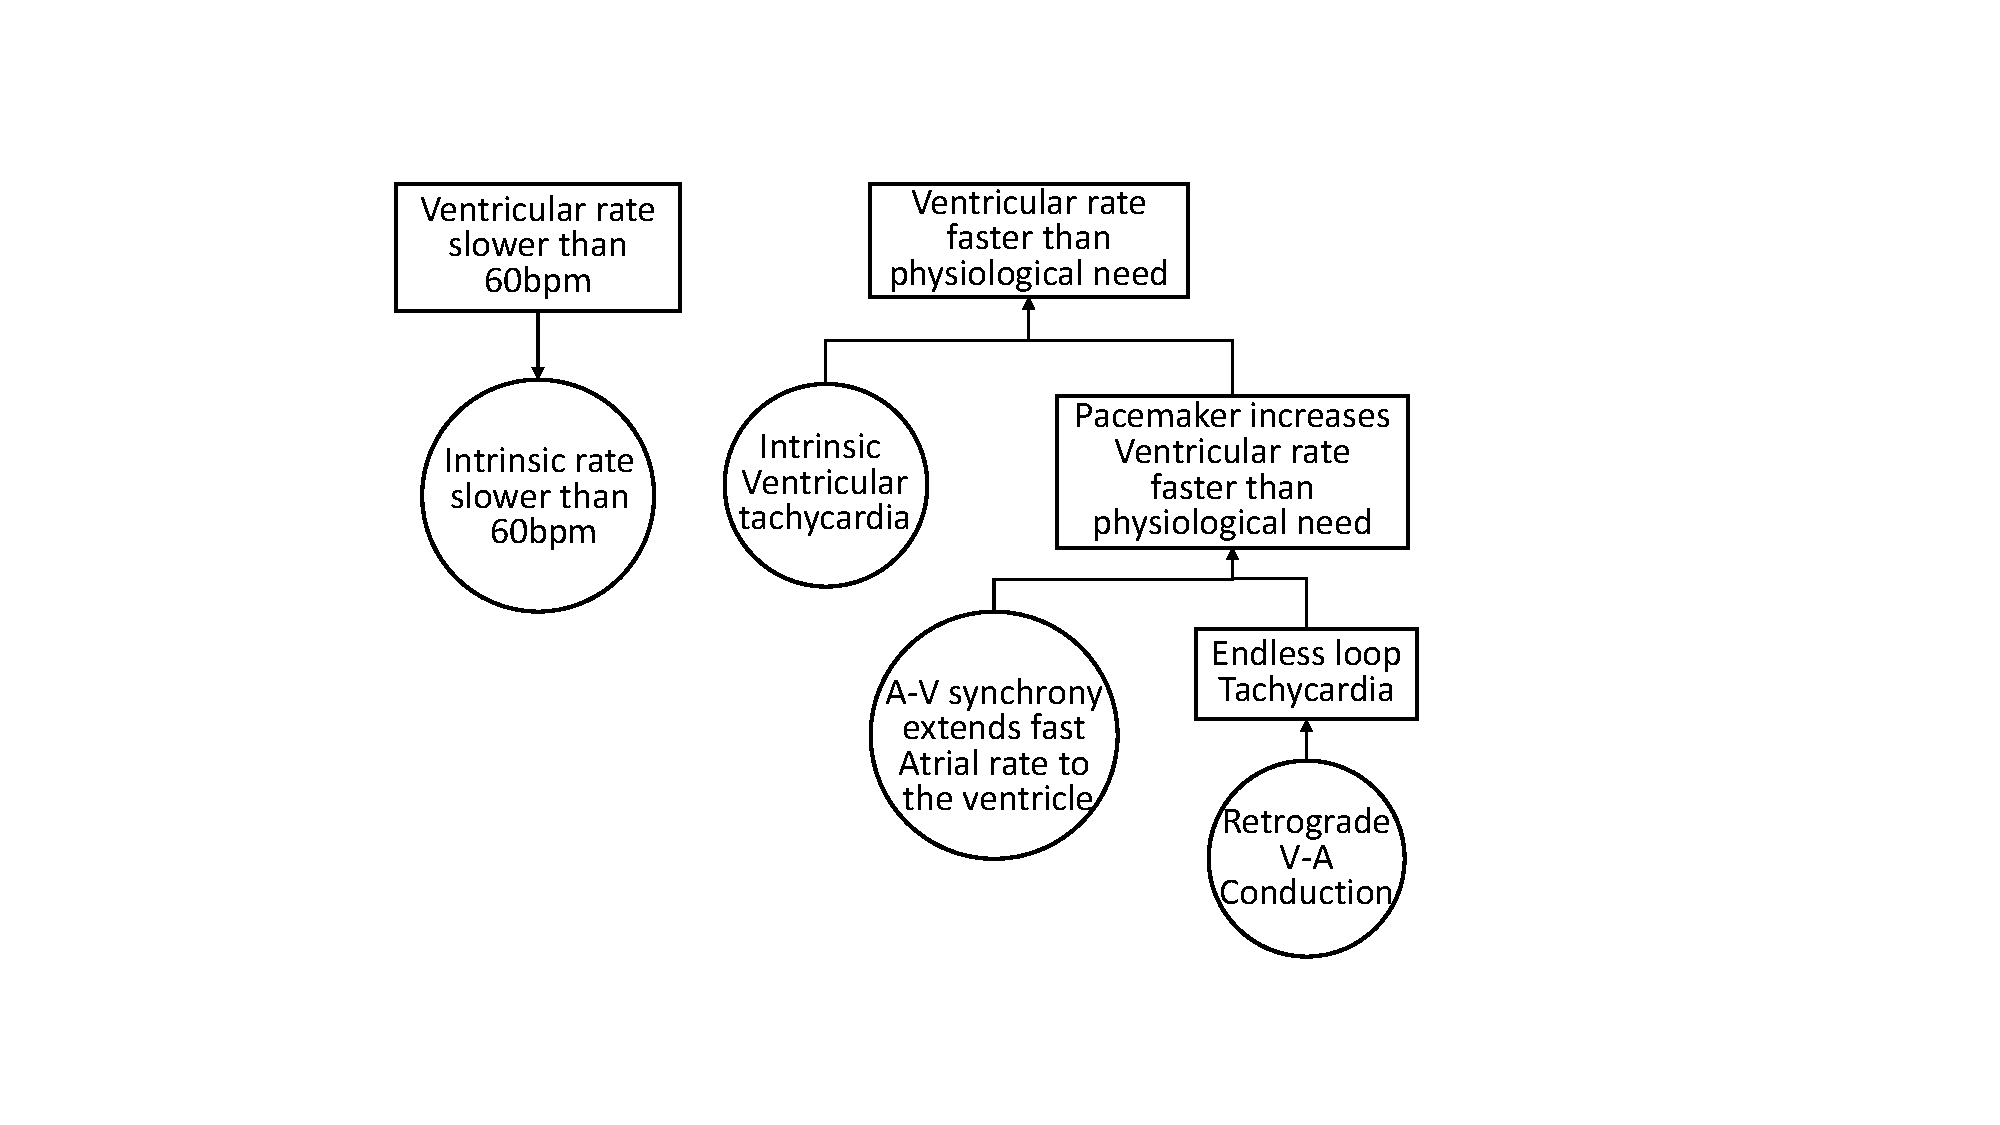
\includegraphics[width=0.8\textwidth]{figs/risk_requirements.pdf}
		\caption{\small Sample Fault Tree Analysis of the physiological conditions leading to the lower rate limit and upper rate limits}
		  %\vspace{-15pt}
		\label{fig:risk_req}
\end{figure}

%            \item What are the effects of adding new features to the software? Can they disrupt the safety properties that the previous device hold?

%In closed-loop model checking, there is only one device model. 
%However there can be a large number of environmental conditions which require different models to represent them. For instance, a heart with atrial flutter has an additional conduction pathway, causing fast atrial rate, that is not present in a healthy heart. The timing and structural differences of different heart conditions should be distinguished in corresponding heart models.
%%\todo[inline]{should we give an example of a heart condition?}
%A set of initial models of the environment can be constructed, but the set is inherently incomplete because of the large number of environment conditions and their combinations. 
%As a result, performing model checking using every model in the set cannot ensure full coverage of the environmental conditions. In the following sections, we will investigate how as we go from basic to more complex requirements, we require more sophisticated approaches to generate and navigate through a variety of environment models. We introduce the concept of an \emph{Abstraction Tree} to systematically encode requirements and choose the appropriate heart models for the requirement. By analyzing the concrete counter-examples we are able to distinguish if the problem is a bug within the device or due to the lack of expressiveness in the environment model. 
\begin{itemize}	
\vspace{-5pt}
	\item How do model checking results fit into the regulation framework?
	\vspace{-5pt}
	\item How do we find the appropriate abstraction level of the environment model for each physiological requirement?
        \vspace{-5pt}
        \item How do we interpret abstract counter-examples returned by model checker?
\end{itemize}
%\section{Testing vs Verification}
%
%\newcommand{\ub}{\bar{u}}
%\newcommand{\yb}{\bar{y}}
%
%\emph{\textbf{Testing}} is a method for checking that a system does indeed obey its specification. 
%In testing, an algorithm will do the following:
%\begin{itemize}
	%\item Initialize the system to some initial state $x_0$ in $X_0$.
	%E.g., for a pacemaker device, this would describe the initial values for the various refractory periods, among other things.
	%\item Generate sequences of input strings $\bar{u}_k$ from some set $A$, in reaction to which the system will produce output strings $\bar{y}_k$,
	%\item A \emph{monitor} logs the output strings and determines whether the pair $(\bar{u}_k,\bar{y}_k)$ satisfies the specification or not.	
%\end{itemize}
%
%Because the set of valid initial states $X_0$ and the set of valid input strings $A$ may be infinite (or simply too large), the test bench must decide on how to intelligently choose a \emph{finite} number of $(x_0,\ub)$.
%They must be chosen such that if the system does not produce wrong behavior with these pairs, then it is unlikely to produce errors under the \emph{full} valid set of pairs, namely, $X_0 \times A$.
%This is the main challenge of testing: how to sample an infinite or large set of behaviors such that it is representative (in the above sense) of the full set of behaviors that $S$ is capable of?
%Another important issue in testing is for how long to test the system: i.e. what should be the length of the $k^{th}$ string $\ub_k$? 
%E.g., if $\ub_k$ has length 1000, the bug might manifest itself on $y_1\ldots y_{1001}$, but not $y_1\ldots y_{1000}$.
%
%Regardless of the testing algorithm, testing remains incomplete, in the sense that short of testing every possible behavior, bugs may lie hidden in the behavior that we did not witness.
%
%\emph{\textbf{Verification}} refers to formal verification.
%It is applicable to finite state systems\footnote{Some infinite-state systems can be formally verified after an abstraction process which essentially produces an equivalent system that has finitely many states.}, 
%and requires formal semantics for the system's operation. 
%Roughly, this means we must have a mathematical unambiguous definition of how the system produces its output.
%A verification algorithm, or \emph{model checker}, will explore the \emph{entire finite state-space} of the system in a systematic manner. 
%Intuitively, if the entire state-space has been explored in all possible ways, and no incorrect behavior has been displayed, then the system is correct. 
%Thus, verification is inherently \emph{complete}: if the model checker determines that the system is correct (under the conditions $A$ and $X_0$), then we can rest assured that is indeed the case.
%Unlike testing, there is no question of whether we missed (didn't run) an initial condition that can display a bug.
%There is also no question of test duration.
%However in practice, some bound on the duration of the verification must be placed to avoid excessively long runs. 
%If the model checker can't determine correctness in that time bound, then the verification is inconclusive.
%
%Verification is computationally expensive and usually more burdensome to setup, but comes with a guarantee on the answer. 
%Testing is computationally cheaper and less burdensome to setup, but the guarantees it provides are significantly weaker.
%Testing, on the other hand, may be the only option for some complex systems that are beyond the capacity of today's model checkers, or which do not possess formal semantics.
%
%In this chapter we cover formal verification of the closed-loop system and address testing in the following chapter.
\section{Risk Analysis for Implantable Pacemaker}
Implantable pacemakers are designed to treat bradycardia by increasing the heart rate with external pacing. Therefore the heart rate should not only be increased to the minimum physiological need, but also should not be increased beyond physiological need. \figref{risk_req} demonstrates two Fault Tree Analysis (FTA) for these two top level hazards. In the remaining chapter we first specify hazards as properties, and use model checking to evaluate whether these hazards have been mitigated by the pacemaker. Then for one of the mitigation algorithm, we examine the mitigation effectiveness and the residue hazard.

\section{Mitigating Top-level Hazards}
The most essential function for the pacemaker is to treat bradycardia by maintaining the ventricular rate above a certain threshold. We define the region where the ventricular rate is slow, as \textsf{unsafe}. The monitor \textsf{PLRI\_test} is designed to measure intervals between ventricular events and is shown in \figref{safety1}. For property
\begin{center}
\textsf{$\varphi_{LRI}=$A[] (PLRI\_test.secV imply PLRI\_test.t$\leq$TLRI)}
\end{center}
we have a closed-loop system  with heart model $H_d$ (described in at the end of Chapter 2): 
$$H_4\| P\| PLRI\_test\models\varphi_{LRI}$$

\begin{figure*}[t]
\centering
%\vspace{-10pt}
		\subfigure[Monitor \textsf{PLRI\_test}] {
				\includegraphics[width=0.5\textwidth]{figs/LRI_test.pdf}
				\label{fig:safety1}
		} 
		\subfigure[Monitor \textsf{PURI\_test}] {	
			\includegraphics[width=0.45\textwidth]{figs/uri_test.pdf}
			\label{fig:uri_test}
		}
		%\vspace{-10pt}
	\caption{(a) Monitor for LRL: Interval between two ventricular events should be less than TLRI, (b) Monitor for URL: Interval between a ventricular event and a VP should be longer than TURI}
\vspace{-10pt}
\end{figure*} 

The pacemaker is not designed to treat tachycardia so it can only pace the heart to increase its rate and cannot slow it down. To mitigate the hazard that the pacemaker may increase the heart rate above physiological need, an Upper Rate Interval (URI) is specified such that the pacemaker can increase the ventricular rate up to this limit. 

\begin{figure}[b]
		\centering
		\includegraphics[width=0.4\textwidth]{figs/vv.pdf}
		\caption{\small Monitor \textsf{Pv\_v} for SVT: There exists an endless sequence in which interval between ventricular events is at most TURI}
		  %\vspace{-15pt}
		\label{fig:vv}
\end{figure}
  
We require that a ventricle pace (VP) can only occur at least $TURI$ after a ventricle event (VS, VP). The monitor \textsf{PURI\_test} is shown in \figref{uri_test}. For the property
\begin{center}
$\varphi_{URI}=$\textsf{A[] (PURI\_test.secV imply PURI\_test.t$\geq$TURI)}
\end{center}
we have: $$H_d\| P\| PURI\_test\models \varphi_{URI}$$

\section{Evaluate the Mitigation}
As described in Chapter \ref{Mode_switch}, the mode switch algorithm has been designed to mitigate the hazard that the A-V synchrony function of DDD pacemaker extends fast
atrial rate to the ventricle. It is important to ensure the effectiveness of the algorithm without inducing other top-level hazards. In this section we first show the existence of the hazard in a pacemaker without the mode-switch algorithm. If the algorithm if effective the hazard will not exist after introducing the algorithm.

\subsection{Existence of Pacemaker Mediated Tachycardia during SVT}
The monitor \textsf{Pv\_v} is designed to show existence of PMT during SVT. It goes to the error state if the ventricular rate drops below the Upper Rate Limit (\figref{vv}).  


We specify 
$\varphi_{MS}=E[] (not Pv\_v.err)$\\
which verifies the existence of PMT. The heart model $H_e$ in Fig. \ref{fig:HM_abs} is not suitable for this property since the non-deterministic conduction of component $P_3$ does not capture the blocking property of the AV node, which is the key in PMT. We use a more refined model $H_d$ which has AV node modeled. To identify the PMT scenario, we first set $H_d.N^1.Trest\_min<100$ so that the atrial rate can be high and $H_d.N^2.Trest\_min>TURI$ so that the intrinsic heart rate is less than TURI. The property is first verified on pacemaker without the mode-switch algorithm. We have $H_d\|P\|Pv\_v\models\varphi_{MS}$ and the evidence returned by the model checker illustrates the PMT scenario.

% There are two separate AVI and LRI components for each mode and switches to the corresponding ones when synchronization signals are received. The clock values are kept so that essential intervals are kept. 
\subsection{Verification against fundamental safety properties}
For a pacemaker with the mode switch algorithm: 

$P_2$=\textsf{LRI'$\|$AVI'$\|$URI$\|$PVARP$\|$VRP$\|$INT$\|$CNT$\|$DUR}, 

we verify the same fundamental safety properties on the pacemaker model with mode-switch algorithm. We have:
$$H_d\|P_2\|PURI\_test\models\varphi_{URI}$$
$$H_d\|P_2\|PLRI\_test\not\models\varphi_{LRI}$$
The Upper Rate Limit property still holds, but the Lower Rate Limit property is violated. The counterexample is proved to be valid after checking the trace of more refined heart models. By analyzing the trace we found that when the pacemaker is switching from VDI mode to DDD mode, the responsibility to deliver VP switched from LRI component to AVI component. Since the clock reference is different (Ventricular events in LRI component and Atrial events in AVI component), the clock value for delivering the next VP is not preserved. As a result, if an atrial event which triggered the mode-switch from VDI to DDD happens within [TLRI-TAVI, TLRI) after the last ventricular event, the next ventricular pacing will be delayed by at most TAVI time, which violates the Lower Rate Limit property (\figref{safety}). 
%%\begin{figure}
%%		\centering
%%		\includegraphics[width=0.4\textwidth]{figs/vv.pdf}
%%		\caption{\small Monitor \textsf{Pv\_v} for SVT: There exists an endless sequence in which interval between ventricular events is at most TURI}
%%		  %\vspace{-15pt}
%%		\label{fig:vv}
%%\end{figure}
\subsection{Verification of the Mode-Switch Algorithm}
After implementing the mode-switch algorithm, we verified the model against the same existence property. We expect the violation of this property, since during VDI mode the ventricular rate of the heart model is less than the Upper Rate Limit and will not trigger ventricular pacing. However, this property is still satisfied, indicating the mode-switch algorithm failed to eliminate the PMT scenario. The evidence trace returned by UPPAAL shows that a subset of atrial events fall into the blanking period after a ventricular event (see \figref{liveness}). As a result, two fast events are reduced to one slow event and mode switch may never happen. This scenario does exist in all our refined heart models, we conclude that the trace is physiologically feasible. The mode-switch algorithm in our pacemaker model can not terminate all PMT behaviors as specified as certain mild PMT events are admissible.
\begin{figure}
\centering
%\vspace{-20pt}
		\subfigure []{
				\includegraphics[width=0.4\textwidth]{figs/safety.pdf}
				\label{fig:safety}
		} 
		\subfigure []{	
			\includegraphics[width=0.4\textwidth]{figs/liveness.pdf}
			\label{fig:liveness}
		}
		\vspace{-10pt}
	\caption{(a) Safety Violation: VP is delayed due to the reset of timer during mode-switch, (b) Correctness Violation: The blocking period may block some atrial events, turning two \emph{Fast} events to one \emph{Slow} event (\cite{TACAS12}})
\vspace{-20pt}
\end{figure} 
\section{Abstraction Tree for Environment Modeling}
In the previous two sections, abstractions and selections of the heart models are performed manually, which require knowledge of both electrophysiology and model checking. 
Counter-examples returned from abstract models can be difficult to interpret by domain experts.
One abstract counter-example could be produced by multiple physiologically valid conditions, which causes ambiguity.
Thus, a rigorous framework is necessary to balance the need to cover a wide range of environmental conditions and the need to provide counter-examples to the physicians within their physiological context. The framework must also allow non-domain experts to perform verification, and establish `hand-off' points where the results of verification can be handed back 
to the experts for interpretation.

In this section, we use a set of domain-specific abstraction rules based on physiological knowledge to ensure the physiological relevance of the behaviors introduced into the abstract models.
The rules are applied to an initial set of physiological models to obtain an abstraction tree, which will be used for closed-loop model checking of the pacemaker. 
A straightforward search procedure is then used to conduct model checking using suitable heart models and return the most concrete and unambiguous counter-examples to the physicians for analysis.
In this framework, physiological knowledge is only needed when constructing the initial model set and when analyzing counter-examples. 
The application of the physiological abstraction rules and the verification procedure can be automated.
The proposed method can potentially be generalized to other domains in which the device operates in a large variety of environmental conditions. More information regarding this research can be found in \cite{regar_tech}.
\subsection*{Step 1: Abstraction Tree construction}
A set of heart models corresponding to different heart conditions are first developed. 
The list can be expanded as new heart conditions are discovered.
Because we start from a set of initial models, and each one may be abstracted using a number of abstraction rules, we have a choice of which rules to apply to which models, and the order in which to apply them. 
Depending on which rule is applied when, we end up with different abstract models.
Thus an \emph{abstraction tree} $T_{HM}$ for the heart is created, as shown in \figref{HM_tree}. 
%Note that applying rules in different order results different abstraction tree. 
%The order used to obtain $HM\_tree$ is based on the domain knowledge that certain heart conditions may have similar behaviors and similar inputs to the pacemaker. 
%This systematic grouping maintains the physiological-relevance of the heart model even at higher abstraction levels, and reduce the necessity to resolve ambiguities at lower abstraction levels when model checking certain requirements.
\begin{figure}[!t]
	\centering
	\includegraphics[width=0.85\textwidth]{figs/abs.pdf}
	%\vspace{-5pt}
	\caption{\small Heart Model Abstraction Tree with arrows showing the direction of the abstraction process starting from detailed models of different heart conditions. Model refinement is in the opposite direction.}
	\vspace{-15pt}
	\label{fig:HM_tree}
\end{figure}

\subsection*{Step 2: Requirement encoding}
The following requirement is designed to prevent the pacemaker from pacing too fast: 
``If the intervals between self-activations of the atria are between 300ms to 1000ms (60bpm - 200bpm), the intervals between ventricular paces should be no shorter than 500ms.''
Self-activation of the atria can be expressed using the location and clock of node automaton $N_A$.
The requirement can be formalized using the monitor  $M_{sing}(VP,500,\infty)$:
%\hatodo{mention $N_A$ is the atrium node automaton}
\[Req1: N_A.loc=Rest \land N_A.t\in [300,1000] \Rightarrow \neg M_{sing}.loc==Err\]
%\todo[inline]{some figure captions are all caps, others are not. please use same thing throughout}
%\begin{figure}[!b]
	%\centering
	%\vspace{-10pt}
	%\includegraphics[width=0.5\textwidth]{figs/abs_sim.pdf}
%
	%\caption{\small Abstraction Rule Application Example}
%\vspace{-10pt}
	%\label{fig:abs_exam}
%\end{figure}
 \subsection*{Step 3: Choosing appropriate heart models for the requirement}
To verify the closed-loop system with pacemaker model $PM$ and abstraction tree $T_{HM}$ (\figref{HM_tree}) against requirement $Req1$, the most abstract appropriate models are selected from the tree. 
The single event monitor $M_{sing}$ from \figref{monitor}(a) with variables $Var(M_{sing})=\{M_{sing}.t,M_{sing}.loc\}$ is used for this requirement. Model checking is performed on the closed-loop system including the heart model $M_H$, the pacemaker model $M_P$, and the monitor $M$. The requirement $\varphi_P$ can be then represented with TCTL formula:
\begin{center}
 \textsf{A[] (not M.Err)}
\end{center}
The variables in the requirement are:
$$Var(Req1)=\{N_A.t,N_A.loc,M_{sing}.loc\}$$
\begin{figure}[b]
		\centering
		\includegraphics[width=0.8\textwidth]{figs/monitor.pdf}
		%\vspace{-5pt}
		\caption{\small (a) $M_{sing}$ for single event; (b) $M_{doub}$ for two events}
		  \vspace{-10pt}
		\label{fig:monitor}
\end{figure}

At the root of the tree $H_{all}$, we have $\{N_A.t,N_A.loc\} \not \subset Var(H_{all})\cup Var(M_{sing})$. 
So $H_{all}$ is not appropriate for $Req1$. 
All the children of $H_{all}$: $H_n'',H_{at}'''',H_{vt}'''$ are appropriate for $Req1$,
%we have $Var(Req1)\cup Var(M_{sing})\subset Var(H_n'')=Var(H_{at}'''')=Var(H_{vt}''')$, 
thus these three heart models are output as the most abstract models that are appropriate for $Req1$.
\begin{figure}[!t]
	\centering
	\includegraphics[width=0.8\textwidth]{figs/abs_rev.pdf}
	%\vspace{-5pt}
	\caption{\small Model refinement: Finding the most concrete counter-examples using the abstraction tree}
	\vspace{-10pt}
	\label{fig:CE}
\end{figure}
	\vspace{-10pt}
\subsection*{Step 4: Return the most concrete counter-examples}
After the appropriate models for $Req1$ are selected, we have the initial set
$HM=\{H_n'',H_{at}'''',H_{vt}'''\}$.
By model checking on all three initial models in UPPAAL we have: 
$$H_n''||PM\not\models Req1;\; H_{at}''''||PM\not\models Req1;\; H_{vt}'''||PM\not\models Req1$$
%$$[1,[]]=ModelChecking(H_n'',PM,Req1)$$
 %$$[0,CE_1]=ModelChecking(H_{at}'''',PM,Req1)$$
%$$[0,CE_2]=ModelChecking(H_{vt}''',PM,Req1)$$
%\hatodoin{In the following text you use $CE_{at}$, etc. It's  best to use the letter subscripts in the above equations as well, so it's clear which cex comes from which heart model.}
%For the two heart models $H_{at}'''',H_{vt}'''$ in which the requirement is violated, the algorithm keeps going down the abstraction tree, and upon termination counter-examples are returned for the following heart models
The abstraction tree is then further explored. The heart models with counter-examples are illustrated in \figref{CE}, and the most refined heart models with counter-examples are: $H_{n};H_{pvc};H_{af};H_{avn};H_{afib}$.
%$$[0,CE_{at}]=ModelChecking(H_{at},PM,Req1)$$
%$$[0,CE_{pvc}]=ModelChecking(H_{pvc},PM,Req1)$$
%$$[0,CE_{af}]=ModelChecking(H_{af},PM,Req1)$$
%$$[0,CE_{avn}]=ModelChecking(H_{avn},PM,Req1)$$
%$$[0,CE_{afib}]=ModelChecking(H_{afib},PM,Req1)$$

%\begin{figure}[!t]
		%\centering
		%\includegraphics[width=0.9\textwidth]{figs/case.pdf}
		%%\vspace{-5pt}
		%\caption{\small Counter-examples}
		  %\vspace{-10pt}
		%\label{fig:CE}
%\end{figure}
	\vspace{-10pt}
\subsection*{Step 5: Analysis of the counter-examples}
The counter-examples are then shared with physicians for analysis. In \figref{CE} we highlight three counter-examples. In the first counter-example, the intrinsic heart signals over time with up arrows as atrial activations and down arrows as ventricular activations. The signal for the second counter-example shows the pacemaker outputs with up arrows as atrial pacing and down arrows as ventricular pacing.%We only show the activations of the atrial node and ventricle pacing. 

Counter-example $CE_{n}$ is returned by $H_n$ and none of its children models violate the requirement. By careful analysis we found that $CE_{n}$ features the combination of fast intrinsic atrial rate and prolonged A-V conduction delay, which is the combination of heart conditions $H_{st}$ and $H_{av}$. This scenario shows that the abstraction rules can introduce physiological heart conditions that were not explicitly modeled in the initial model set. The pacemaker improved the open-loop heart condition by pacing the ventricles $AVI$ after each atrial event, which is a correct operation of the pacemaker despite the requirement violation. 
%\hatodo{is it TAVI or AVI like in the previous seciton?}

%\hatodoin{Do you mean that $CE_{at}$ is not a bug? Does this mean that the requirement may be violated in ways that are not dangerous?}
Counter-example $CE_{pvc}$ has a very similar execution to $CE_{n}$. However, the activations of the atrial node are triggered by retrograde conduction from ventricle to the atrium initialized by ventricular paces (marker \textsf{cond}). The atrial activations trigger another ventricular pace after $AVI$, which will trigger another retrograde conduction. In this case, the heart rate is inappropriately high, which corresponds to a dangerous closed-loop behavior referred to as \emph{Endless Loop Tachycardia}.

In counter-example $CE_{af}$, the atrial rate is very high, which is also a sub-optimal but not dangerous heart condition. 
However, the ventricular rate can stay normal due to the blocking property of the AV node. 
Despite the filters in the pacemaker, the pacemaker still paces the ventricle for every 3 atrial activations, which extends fast atrial rate to more dangerous fast ventricular rate. 
%\hatodoin{Not very clear..do you mean that the intrinsoc centricular rate is fine because of AV filtering, but the PM is accelarating it?}
This scenario is referred to as Atrial Tachycardia Response of a pacemaker. 

From the analysis, pacemaker operations in $CE_{pvc}$ and $CE_{af}$ must be revised. However, the revision should not affect the behavior in $CE_{n}$. This example demonstrates that counter-examples from refined models provide more physiological context of the requirement violations, and distinguish the physiological conditions that can trigger the violations. The information is helpful for debugging and improving the algorithm. The physicians can also improve the physiological requirement so that these heart conditions can be then considered case by case.\\

\noindent\textbf{Discussion:}\\
Model checking is not widely use in industry, in part, due to scalability issues and also because domain expertise must be a skill possessed by the verification engineer. However, with rigorous abstraction of the system and its environment, model checking can be used to identify 
known and even unknown mechanisms to induce hazards. In this chapter, we use a model of a dual chamber pacemaker as an example to demonstrate the use of model checking during risk analysis. During the process we identified the need to refine the heart models to eliminate false-positives introduced during the abstraction, and demonstrated the difficulty to do so manually. The abstraction tree approach is then proposed to reduce the effort needed for both the developers and the domain experts, which makes model checking a viable approach for providing safety and effectiveness evidence. 

\chapter{Theme 3: Verified Model to Verified Code}
Model checking is performed on abstract models of the system, which is at an early stage in the development process. The verified system model during model checking is then translated into a Stateflow model, which is a step towards simulation-based testing and subsequently to code generation. Closed-loop simulation/testing are performed on more refined deterministic models, and on the actual system, complement model checking in terms of resolving ambiguities within abstract counterexamples. We aim to answer the following questions here:

\begin{itemize}
	\vspace{-5pt}
	\item How are abstract models translated to deterministic models for simulation-based testing?
	\vspace{-5pt}
	\item What system level issues are best tested at the platform level?
\end{itemize}

In this chapter, we first describe an approach to automatically translate formal models that are verified in UPPAAL to Stateflow charts for simulation-based testing, and then code generated to run on an embedded platform. Following this, we demonstrate two examples that cannot be explicitly modeled using abstract semantics and must be tested.

\section{UPPAAL to Stateflow Automated Model Translation}
%%%%%%%%%%%%%%%%%%%%%%%%%%%%%%%%%%%%%%%%%%%%
\begin{figure*}[!b]
\centering
		\subfigure 
		{			
		\includegraphics[width=0.45\textwidth]{figs/method_new1.png}		
		\label{fig:method}
		}
		\hspace{.2in} 
		\subfigure 
		{	
			\includegraphics[width=0.45\textwidth]{figs/chart_GlobalClocks_rev1.png}
			\label{fig:chart}
		}
\caption{(a)~Model Driven Design framework: From UPPAAL to Stateflow to generated code -- covering model verification, simulation-based testing and platform testing.~(b) Structure of Stateflow charts of the pacemaker's five basic timing cycles (from Fig. \ref{fig:PMdesign}) derived by the UPP2SF model translator. Parent states $P_1,...,P_n$ are derived from automata, while the \textit{clock} states $Gc\_{x_1},..., Gc\_{x_m}$ model all global clocks $x_1,...,x_m$ from the UPPAAL model. The state $Eng$ is used to control execution of the chart.}
\label{fig:upp2sftool}
\end{figure*} 
%%%%%%%%%%%%%%%%%%%%%%%%%%%%%%%%%%%%%%%%%%%%

A model translation tool, UPP2SF (\cite{TECS}) was developed to translate UPPAAL models to Stateflow (see \figref{method}). Consider an UPPAAL model with automata $P_1,...,P_n$.  After UPP2SF translation, a two-level Stateflow chart is generated as in \figref{chart}. The chart consists of parallel states $P_1,...,P_n$ (referred to as the \textit{parent} states) derived from the automata, parallel states $Gc\_{x_1},..., Gc\_{x_m}$ (referred to as \textit{clock states}) that model all global clocks $x_1,...,x_m$ from the UPPAAL model, and the state $Eng$ that is used as the chart's control execution engine.
Moreover, the chart has predefined global data variables (and constants) with appropriate ranges and initial values derived from the UPPAAL model. 
Since all automata in UPPAAL are active simultaneously, the obtained Stateflow chart is a collection of parallel states with unique execution orders. Also, in every UPPAAL automaton exactly one location is active at a time. Thus, each of the parent states is a collection of exclusive states, extracted from locations in the corresponding UPPAAL automaton. 

In \cite{TECS}, we showed that for a large class of UPPAAL models, the generated Stateflow models generated by UPP2SF preserve behaviors of the initial UPPAAL models. The translation tool can be used to estimate the worst case execution time (WCET) during modeling and model checking stage in UPPAAL, and facilitates development of modular code from timed-automata based models. 

%%\begin{figure} [!t]
%%\center
%%\includegraphics[width=0.48\textwidth]{figs/chart_GlobalClocks_rev1.png} 
%%\caption{}
%%\label{fig:chart}
%%\end{figure}

\figref{PM_sf} demonstrates the Stateflow chart generated from the UPPAAL model of the DDD pacemaker model in \figref{PMdesign} using the UPP2SF tool.
\begin{figure*} [!t]
\center
\includegraphics[width=0.77\textwidth]{figs/PM_SF_buffer_newC1.png} 
\caption{Pacemaker Stateflow chart converted from the UPPAAL model in~\figref{PMdesign} using UPP2SF; the heart and buffer models are highlighted.} 
\label{fig:PM_sf}
\end{figure*}
We generated C code from the pacemaker Stateflow chart using the Simulink Coder. The code structure is shown in \figref{pm_code}.
The code was generated for the general embedded real-time target and as a result we obtained the main procedure, \texttt{rt\_OneStep}, which processes the three input events, $VinB$, $AinB$ and $clk$. To ensure that the model semantics are preserved (modulo the execution time), $clk$ input events should be created every 1ms, followed by the procedure's activation. This makes it suitable for implementation on top of a real-time operating system (RTOS).

\begin{figure*} [!t]
\center
\includegraphics[width=\textwidth]{figs/CodeListingFinal.png}
\caption{Structure of the pacemaker code obtained from the Stateflow chart shown in \figref{PM_sf}.}
\label{fig:pm_code}
\end{figure*}


The pacemaker code generated by the Simulink Real-Time Workshop's Embedded Coder was executed on nanoRK (\cite{nanork}), a fixed-priority preemptive RTOS that runs on a variety of resource constrained platforms. We tested the implementation on the TI MSP-EXP430F5438 Experimenter Board interfaced with a signal generator that provides inputs for the pacemaker code (\figref{setup}). More details regarding UPP2SF translation and platform testing can be found in \cite{TECS}.

%%%%%%%%%%%%%%%%%%%%%%%%%%%%%%%%%%%%%%%%%%%%
\begin{figure*}[!t]
\centering
		\subfigure 
		{			
		\includegraphics[width=0.46\textwidth]{figs/HM_PM_newMon.png}
		\label{fig:hm_pm}
		}
		\subfigure 
		{	
			\includegraphics[width=0.48\textwidth]{figs/HW_setup1.png}
			\label{fig:PM_timer}
		} 
\caption{(a)~Structure of the pacemaker model in UPPAAL and Stateflow, including the interaction between the pacemaker and heart, and the monitors used for verification. (b) Hardware setup with MSP430F5438 experimenters board.}
\label{fig:setup}
\end{figure*} 
%%%%%%%%%%%%%%%%%%%%%%%%%%%%%%%%%%%%%%%%%%%%



\subsection{Summary:}
In this chapter, we first introduced a model translation method from UPPAAL timed automata models to Stateflow charts. Combined with Simulink coder, the tool chain provides rigorous evidence of traceability from physiological requirements to the C code implementation. Oversensing, crosstalk and lead displacement are three examples in which the cause of the problem is not modeled in the abstract interface in the timed-automata model. In such cases, closed-loop testing with the more refined heart models and EGM interface can be used to provide safety evidence.


%\subsection{Acknowledgements}
%\begin{acknowledgements}
%\addcontentsline{toc}{chapter}{Acknowledgements} 
%The authors would like to thank Houssam Abbas, Rajeev Alur, George M. Chen, Allison Connolly, Sanjay Dixit, Insup Lee, Pieter Mosterman, Miroslav Pajic, Oleg Sokolsky and Larisa G. Tereshchenko for fruitful discussions during the preparation of this manuscript. This research was supported in part by NSF CNS-0720518, NSF CNS-1035715, NSF MRI-0923518, NSF CPS Frontier 1446664 and NSF CAREER-1253842 grants. This work was also supported in part by STARnet - a Semiconductor Research Corporation program sponsored by MARCO and DARPA.
%\end{acknowledgements}
%%\chapter{Certification}
%%\begin{itemize}
%%          	\item What is the current practice for medical device certification? What are the limitations?
%%          	\item Can model-based closed-loop verification provide more safety guarantee to complement current practice? By how much?
%%          \end{itemize}
%%          
%%\section{Current Practice}
%%%In United States, medical devices have to be approved by FDA to be released into the market. 
%%According to their potential risks the devices are categorized into 3 classes, Class I, Class II and Class III, corresponding to low-risk, medium-risk and high-risk devices \cite{class}. Life-sustaining devices like implantable pacemakers are classified as Class III and in general are subject to the most strict regulations.
%%
%%There are two processes that a medical device can enter the market in U.S.: the Premarket Notification, also known as 510(k) \cite{510k}, and the Pre-Market Approval (PMA) \cite{PMA}. In a 510(k) submission the device manufacturers are only required to provide evidence that the device is \emph{substantial equivalent} to a \emph{predicate device}, which has been approved for the market. Therefore, the 510(k) submission does not directly require clinical evidence for the safety and effectiveness of the device, thus is suitable for mostly low-risk devices like Class I and Class II devices.  The Pre-Market Approval (PMA) submission is a more stringent regulatory process in which direct clinical evidence is required to prove the safety and effectiveness of the device. However, not all Class III devices are subject to PMA submission. If a Class III device clears the 510(k) process and FDA has not requested PMA for that device, the device is still cleared for market release. A study shows that for Class III devices which PMA has been requested, the levels of evidence varies. Only 40\% of the PMA submissions are supported by controlled clinical trials, which provide the most rigorous clinical evidence \cite{cert_prob}. The lack of quality evidence is usually due to the high cost of the controlled clinical trials.
%%\section{Evidence from Model-based Design}
%%%\cite{pancreas}
%%Model-based verification provides a low-cost solution to provide reasonable evidence for the safety and effectiveness of the devices. The open questions are:
%%
%%\begin{itemize}
%%	\item How valid are the models?
%%	\item How much confidence can they provide?
%%\end{itemize}

\chapter{Theme 4: in-silico Pre-clinical Trials for Implantable Cardiac Devices} 
10,000 people in the U.S. receive an Implantable Cardioverter Defibrillator (a heart rhythm adjustment device) every month \cite{asktheicd}.
Clinical trials have presented evidence that patients implanted with ICDs have a mortality rate reduced by up to 31\% \cite{maditrit}.
Unfortunately, ICDs suffer from a high rate of \emph{inappropriate therapy}, which takes the form of unnecessary electric shocks or pulse sequences delivered to the heart.
Inappropriate therapy increases patient stress, reduces their quality of life, and is linked to increased morbidity \cite{shock_mortality}.
Depending on the particular ICD and its settings, the rates of inappropriate therapy range from 46\% to 62\% of all delivered therapy episodes \cite{GoldABBTB11_RIGHTresults}.
	\begin{figure}[t]
		\centering
		\includegraphics[scale=0.5]{figures/figTransResearchSpectrum.pdf}
		\caption{\small Bringing a device to market.
			Clinical trials are the last step before a new device's market approval.
			Model-based clinical trials will provide insight during planning and execution of clinical trials, leading to reduction in costs and increasing the chance of a successful trial.}
		\label{fig:spectrum}
	\end{figure}

%The closed loop formed by the organ (heart) and device (ICD) is an example of a life-critical Cyber-Physical System (CPS): the device's software is the cyber component, and the physiological phenomenon (e.g., cardiac rate and electrical activity) is the physical component.
%\headline{The technology in some of these devices combines hardware and software, each of which must be rigorously verified to be efficacious and safe.}
%\headline{In this paper we are concerned with \emph{closed-loop devices}.}
%Such a device is in a feedback loop with the organ(s) it effects (see Fig.\ref{fig:pacemaker}): an ICD for example monitors the heart rate, and delivers therapy to maintain an adequate rate.
%Another example is the artificial pancreas, which monitors blood glucose levels and delivers insulin to maintain safe glucose levels.

\emph{After the verification and testing effort is completed}, regulatory agencies like the F.D.A. require that the safety and efficacy of new devices be demonstrated in a \emph{CT} (Fig.~\ref{fig:spectrum}).
%\footnote{In this paper, we always mean a randomized controlled trial, which is the type of trial described here.}
In a trial, a group of patients that are treated with the new device (this is the `intervention group') are compared to a group of patients who are treated with the current standard of care (e.g., a different device currently on the market; this is the `control group').
The objective is to see whether the different devices result in significantly different effects on the patients.
Clinical trials are major endeavors, involving physicians, patients, statisticians, clinical centers, companies and regulators, sometimes in several countries.
Late-phase trials can run for several years, and cost millions of dollars.
For example, a 2002 trial for stents lasted 2 years, enrolled 800 patients and cost \$10 to \$12 million and lasted 24 months \cite{Kaplan04_Cost}.
Trials also pose an inherent risk to the patients in the intervention group by exposing them to an unproven device.
Thus it is crucial that they be well planned, and rigorously executed.

In reality, any trial runs the risk of errors during its planning and execution stages, which can invalidate the results of the trial.
In this paper, we pose and propose an answer to the following question: \emph{how can modeling of CPS assist in the planning and execution of a clinical trial, so as to increase the chances of a successful trial}?
%The advent of computer models for various physiological functions defines a new convergence point for computer science and engineering with medicine.

Most medical models today are aimed at either better understanding the phenomenon under study \cite{vfiborganization_Tusscher07} or at device debugging and verification \cite{VHM_proc}. 
There is only one case in which a computer model has been used to intervene in the regulatory process of medical devices, namely the T1 Diabetes Model (T1DM) of UVA/PADOVA \cite{T1DM}.
T1DM models glucose kinetics in hypoglycemia, and has been accepted by the FDA as a substitute for animal trials.
The T1DM has a fixed virtual cohort with 300 patients.
Its objective is to test the efficacy of new glucose control algorithms by simulating them on the virtual cohort.
While our models can be used in this way, our objective here is to target specific clinical trials steps and improve how they are conducted.
This dictates the experimental setup and the cohort generation considerations.

The Avicenna consortium \cite{Avicenna} lays out a vision for `In-Silico Clinical Trials' similar to our approach.
However, the emphasis in Avicenna is on individualized patient models, as they propose to customize the model to each patient enrolled in a trial.
In the present work, we propose a usage of MBCT \emph{prior} to recruitment.
Thus our models need not be fitted to a given patient's data, which might be impossible, invasive, or burdensome for the conduct of the trial.

In this chapter,
we demonstrate how  computer models can be used for early, affordable and reproducible testing of a clinical trial's premises and assumptions.
Model-based empirical validation of the premises reduces the risk of conducting a trial that fails to demonstrate the desired effect (typically, an improvement of new intervention over the control). 
We used the Rhythm ID Going Head to Head Trial (RIGHT) \cite{GoldABBTB11_RIGHTresults}, which lasted five years and sought to compare the diagnostic algorithms used by two ICDs for correctly diagnosing potentially fatal tachycardias (abnormally fast heart rhythms).


\section{Clinical trials and RIGHT}
\label{sec:rcts}

At the clinical trial stage (Fig.~\ref{fig:spectrum}), the objective is no longer to find bugs in the device: it is, rather, to evaluate the safety and efficacy of the validated device on humans. 
RCT are the gold standard for evaluating the safety and efficacy of a new medical device \cite{FriedmanFD10_ClinicalTrials}.
They constitute the only time prior to market use where the effects of the device on humans are actually observed, and are legally mandated for new high-risk medical devices like ICD.
%It is important to understand how a typical RCT proceeds to appreciate where CPS modeling can help in that process.
%Very broadly, in an \ac{RCT}, a new treatment also known as the \emph{intervention}, is compared to the current standard of care, commonly known as the \emph{control}.
%For example, two competing ICDs are compared.
%Each patient recruited to the trial is randomly assigned to either the intervention or the control group and undergoes the corresponding treatment.
%At the end of the trial, any clinically relevant differences between the two groups are evaluated to determine if they are statistically significant.
The planning and execution of an RCT requires carefully navigating a number of technical, logistical and ethical issues to obtain reliable and statistically significant results.

Because of the very high cost of RCT in terms of money, time, and the risk of harm they present to enrolled patients, our focus in this paper is on the use of CPS models, formalized in an MBCT, \emph{to validate the assumptions made by the investigators and thus increase the chances of success of an RCT}.
We illustrate our approach by applying it to the Rhythm ID Going Head-to-Head Trial (RIGHT) \cite{GoldABBTB11_RIGHTresults}, which we present next.
\begin{figure}[tb]
	\includegraphics[scale=0.6]{figures/figICD.pdf}
	\caption{ICD connected to the heart. The atrial, ventricular, and shock electrogram signals are measured by the device, which uses them to diagnose the current state of the heart and determine whether therapy is required.}
	\label{fig:icd}
\end{figure}

\subsection{The RIGHT trial}
\label{sec:right}
We first provide a brief background to better understand RIGHT. Tachycardias (abnormally elevated heart rates) can be divided into VT, which originate in the heart's ventricles, 
and SVT, which originate above the ventricles.
A sustained VT can be fatal, while an SVT is typically non-fatal.
The therapy applied by the ICD often takes the form of a high-energy electric shock.
The shock can be pro-arrhythmic, and was even linked to increased morbidity \cite{shock_mortality}.
Therefore, one of the biggest challenges for ICDs is to guarantee shock delivery for VT, and simultaneously reduce inappropriate shocks during SVT \cite{Ellenbogen11_Pacingbook}.

RIGHT is a trial that sought to compare the VT/SVT discrimination abilities of two algorithms \cite{GoldABBTB11_RIGHTresults}: 
the Rhythm ID detection algorithm found in Boston Scientific's Vitality II ICDs~\cite{compass},
and the PR Logic + Wavelet (PRL+W) detection algorithm found in a number of Medtronic's ICDs (Medtronic Maximo,
Marquis, Intrinsic, Virtuoso, or Entrust ICD).
%\mynote{SD}{make sure to list all the Boston Scientific and Medtronics ICD models that use each of these algorithims. This is very important}
%The investigators chose the following primary question: is there a difference in time-to-first inappropriate therapy between the two ICDs?
\emph{Inappropriate therapy} was defined as therapy applied to an arrhythmia other than VT or VF (VF is a type of VT).
RIGHT enrolled 1962 patients and ran for approximately five years.
It was fully sponsored by Boston Scientific. 

One of the trial's assumptions was that Rhythm ID would reduce the risk of inappropriate therapy by 25\% over PRL+W~\cite{Berger06_RIGHT}.
The outcome of the trial~\cite{GoldABBTB11_RIGHTresults}, however, was that patients implanted with ICDs running Rhythm ID had a \emph{\textbf{34\% risk increase}} of inappropriate therapy as compared to patients implanted with ICD running PRL+W. 
This result  is the opposite of the effect hypothesized by the trial investigators. 
In this paper, we design an MBCT to test early and quickly whether the hypothesized effect holds by comparing the two ICDs on a large \emph{synthetic} cohort.\\\\
\textbf{\emph{Organization:}} In the following sections we describe the building blocks of in-silico pre-clinical trials: modeling the heart, processing 100's of real patients' data, mapping the timing and morphology components of the signal to a heart model we developed, generating a population of 10,000+ synthetic heart models, implementing the device algorithms and conducting multiple trials for the comparative rate of inappropriate therapy, condition-level rates and evaluating the effect of device parameters on discrimination rates.

 \section{Virtual Cohort Generation}
 \label{sec:heart modeling}
%The first step in any MBCT is to choose a patient model that can interact with the device in a closed loop. 
%Computer models of the heart have been developed to model different aspects of the cardiac function to suit different applications (\cite{natalia,Grosu_wave}).
%In this section we first give a brief overview of the basic Electrophysiology of the heart which describes the electrical activation and conduction, which is the basis for ICDs. 
%We also describe our effort to model the electrical activity of the heart to generate signals corresponding to a large range of heart conditions that the ICD can encounter.

Implantable Cardioverter Defibrillators (ICDs) can diagnose VT and VF by observing the electrical activity through three channels, as shown in Fig.~\ref{fig:icd}.
The measured signals are known as \emph{electrograms}, or EGMs.
VT and SVT can share similar heart rates and might even occur simultaneously, so an SVT can be mis-diagnosed as a VT. 
This is problematic because VT therapy consists of low and high energy electric shocks of 30-40 Joules ($\sim$800V) delivered directly to the heart, which is very painful to the patient, and has been shown to increase morbidity \cite{shock_mortality}\footnote{\small{Physicians compare a shock to a ``horse kicking you in the chest"}}.
Therefore, one of the biggest challenges for ICDs is to discriminate between VT that typically requires a shock, and SVT that typically should not be shocked \cite{Ellenbogen11_Pacingbook}.

An EGM signal can be characterized by the \emph{timing of events} that produced it, and the \emph{morphology of the signal itself}.
An `event' is roughly characterized as the source of the largest peak in the EGM (e.g. a ventricular depolarization), and event timing is a crucial element of an arrhythmia's definition in clinical Electrophysiology.
The `morphology' refers to the shape of the EGM (see Fig. \ref{fig:adjudication} for examples).
Both aspects are used by the ICD to make its decision.
Correspondingly, our model has two components: a timing model, and a morphology model.

\subsection{Timing Model}
\begin{figure}[t]
	\centering
	\includegraphics[width=0.8\textwidth]{figs/HM_top.pdf}
	\caption{\small Timing model of the heart}
	\label{fig:HM_top}
\end{figure}

The node and path topology used in the MBCT is shown in Fig. \ref{fig:HM_top}. 
The hollow nodes are passive nodes representing key locations within the heart where electrical events may be blocked. These include the Atrioventricular node (AV), Right Bundle Branch (RBB) and Left Ventricle Apex (LVA). 
The filled nodes in red, Sinoatrial (SA) node and Right Ventricle Apex (RVA) node, represent the heart locations where ICD electrodes are placed to measure the EGMs.
The timing of the activation events at these nodes determines the timing of corresponding EGMs.
Different sources for tachyarrhythmias are represented by arrhythmia nodes (dashed filled nodes) which are capable of self-activating at prescribed rates. These include Premature Atrial Complexes (PACs) and Premature Ventricular Complexes (PVCs) which are sources of rhythm disturbances.

Every node and path automaton has timing parameters that determine, for example, the delay between events, and how long it takes to conduct an electrical event between two nodes.
These timing parameters can be directly derived from clinical data \cite{josephson}, and the model structure is compatible with clinical Electrophysiology concepts.
Thus we know the ranges for these parameters.
In \cite{VHM_proc}, the timing model's capability to simulate various normal and abnormal heart conditions was validated quantitatively and by cardiac electrophysiologists.


In this work we use the same heart model structure to ensure the correct timing of the EGM signals into the ICD.
%The nodes in orange are capable of self-activation at different rate determined by corresponding parameters, which represent different sources for tachy-arrhythmia.
%Since in this study we do not need the heart models to react to device therapy.
In order to account for inherent timing variability, during simulation the heart model randomly selects timing parameters within a pre-specified range, instead of choosing specific values. 
By choosing the range, we control the variability of the signals produced by a given model instance.

\subsection{Morphology Model}
The ICD uses the EGM morphology in two ways:
first, the atrial and ventricular EGMs are used to \emph{sense} when events occur via peak detection (Section \ref{sec:sensing}).
Second, the Shock channel EGM is used in the morphology comparison discriminators (Section \ref{sec:svtvt}, \cite{VTC,Wavelet}).
It is known that sensing (the detection of events) can be responsible for up to 20\% of inappropriate therapies \cite{wrong_sensing}.
Therefore, it is important that our model generate realistic and varied EGM waveforms for a proper evaluation of the detection algorithms.

\begin{figure}[t]
	\centering
%	\vspace{-5pt}
	\includegraphics[scale=0.4]{figures/figEGMGeneration1column.pdf}
	\caption{\small EGM waveform generation.
		From a given model instance and set of tachycardias, an EGM waveform is generated for the duration of an episode. The timing model determines event timings. When an event occurs, the EGM morphology for the event is output from the morphology model.  
		}
	\label{fig:egmGeneration}
\end{figure}
The timing model provides the time stamps for electrical events to happen at the interfacing nodes (SA,RVA). 
From path conduction we also know the source of the signals.
In the heart model structure shown in Fig. \ref{fig:HM_top} there are 5 different sources for SA node activation and 5 different sources for RVA node activation. 
Based on the clinical observations that electrical events from the same source produce very similar EGM morphologies, we can generate EGM signals by overlaying EGM templates corresponding to different sources onto the timing event diagram.
The procedure is shown in Fig. \ref{fig:egmGeneration}.
We also introduce small variations on EGM templates.
The variations are obtained by a wavelet decomposition of the signatures followed by a random scaling of the 25\% smallest coefficients.
We guarantee that this does not change the signature of the EGM, by running one of the morphology comparison discriminators described in Section \ref{sec:svtvt}.
This variation is parametrized, e.g. the percentage of modified coefficients, the range of the random scaling.

\subsection{Patient Data Adjudication and EGM Template Extraction}
In order to obtain realistic morphologies for our simulations we utilize the Ann Arbor Electrogram Libraries (AAEL), a database of over 500 EGM recordings made during clinical electrophysiology studies~\cite{AAEL}. 
The AAEL is used by all major ICD manufacturers and is licensed by the US FDA. 
The AAEL provides descriptive annotations of records at a high level.
We performed additional detailed examination to precisely segment each record according to rhythm type.
123 records from 47 patients were manually examined and adjudicated into segments called \emph{episodes} containing one specific rhythm, e.g. NSR or VF. 
The adjudication was performed by a cardiologist.
Fig. \ref{fig:adjudication} (left) shows an example record (Record A185660) which has undergone this adjudication.
%It should be noted that only with a standard 12-lead \ac{ECG} in addition to ICD signals can all types of arrhythmia be accurately diagnosed.
From each episode, we developed an automated process which extracted EGMs from a given episode. 
The EGM are collected and organized by both patient record and by the type of rhythm which was annotated during the adjudication process.
These extracted rhythm \emph{signatures} provide the basis for the morphology information in the signal generated by our model.
Fig. \ref{fig:adjudication} (right) depicts an example of 10 signatures extracted from the record. 

\begin{figure*}[t]
	\centering
	\includegraphics[scale=0.35]{figures/figadjudication.pdf}
	\caption{\small  (Left) The EGM record is segmented into episodes with distinct rhythms in each. (Right) From each episode, individual EGM morphologies are extracted and stored.
	}
	\label{fig:adjudication}
\end{figure*}

\subsection{Cohort generation}
\label{sec:cohort generation}
Let $p = (p_1,\ldots,p_n) \in \Re^n$ be the vector of timing and morphological parameters of the heart model.
Let $P_i \subset \Re$ be the range of parameter $p_i$.
We generate a \emph{synthetic cohort} of $N$ probabilistic model instances.
To produce one of these instances, for each scalar parameter $p_i$, we randomly select a sub-interval $I_i$ of its range: $I_i \subset P_i$.
The sub-interval $I_i$ is chosen so that it fits with the tachycardia that this model instance is meant to simulate.
E.g., for modeling VT, the rest period of the VT node might be assigned the sub-interval $I_i = [260, 280]ms$, reflecting the firing rate in the ventricles.
%Two different instances of the same tachycardia will, in general, have different sub-intervals within $P_i$.
When a model instance is simulated, each parameter $p_i$'s value changes beat to beat by sampling it uniformly within its sub-interval $I_i$.
Thus each generated model is probabilistic to reflect inherent rhythm variability.

\section{Implementing Device Algorithms} 
\label{sec:device models}
Due to the limited sensing capability of ICDs, device manufacturers have developed different algorithms to identify the electrical events and correctly diagnose the cardiac arrhythmia as being VT or SVT.
In this paper we implemented the detection algorithm Rhythm ID of Boston Scientific \cite{compass,Ellenbogen11_Pacingbook},% [???Compass, pacingdefibrillation,VTC paper, ICD book, Ellenbogen].
and PRLogic+Wavelet (PRL+W) of Medtronic \cite{Singer,Wavelet}.
%In available literature on the evaluations of device algorithms descriptions of the device algorithms are not detailed enough for full implementation.
%To obtain the detailed implementation we further reviewed clinical execution traces from literature like \cite{Singer} to infer detailed executions of the algorithms. 
We also set up a testing platform to validate our implementations against real ICDs using conformance testing.
\subsection{Cardiac Signal Sensing}
\label{sec:sensing}

%Basic definition and principle
\emph{Sensing} is the process by which cardiac signals measured through the leads of the ICD is converted to cardiac timing events.
Appropriate sensing is essential for proper ICD detection algorithm operation which relies heavily on accurate event timing and morphology information provided by sensing. 
An \emph{event} corresponds to a depolarization in the heart and manifests as a displacement from the baseline amplitude of the signal.
In its simplest form, the sensing algorithm declares an event whenever the amplitude of the signal exceeds a given threshold.
Once an event has been declared, the peak of the amplitude is measured and a \emph{refractory period} begins, during which a consecutive event is ignored for a short period of time. 
This is to ensure that the same event is not counted repeatedly.

%Difficulty of sensing
ICDs require a balance in sensitivity in order to operate in noisy, complex, environments where cardiac events can vary greatly in signal amplitude and frequency, such as during VF. 
Setting the threshold low achieves higher sensitivity to events of small amplitude, but increases the chances for incorrectly sensing other cardiac electrical artifacts such as T-waves and noise artifacts (oversensing). 
Conversely, setting the threshold too high allows sensing to be more robust to noise and other cardiac electrical events, but creates the potential for undersensing events of interest, such as during VF when the peak amplitude can be low. 

%Enhancement 1: 
In order to achieve adequate balance, ICD sensing algorithms are enhanced by applying dynamic adjustment of the sensitivity threshold.
Initially, the threshold is raised during the refractory period after an event and once the refractory period concludes, the threshold is decayed to a minimum pre-set threshold.
In our device models, we implemented the AGC algorithm of Boston Scientific and the AAS of Medtronic ICDs to incorporate dynamic threshold adjustment. 

%%Enhancement 2: Cross-chamber blanking
%In addition to \ac{AGC}, in our device model for Boston Scientific, we have implemented a specific \emph{cross-chamber blanking} feature present in Boston Scientific \ac{ICD}s. 
%Cross-chamber blanking starts a blanking period in atrial sensing after a ventricular event has been detected.
%This reduces the chance of a ventricular event being interpreted as an atrial event.

The complexity of these enhancements adds to the difficulty of properly programming device settings of ICDs and requires calibration process at the time of ICD implantation and during patient follow-up visits.
\subsection{VT Detection Algorithm}
\label{sec:svtvt}
%The limited sensing resolution and noise in the \ac{EGM} signals make it is impossible for the device to achieve 100\% accuracy for SVT/VT discrimination.
Device companies have developed different algorithmic components to distinguish SVT from VT, referred to as \emph{discriminators}. 
Each discriminator utilizes the history of timing and/or morphology of the EGM signals to determine whether the current rhythm is a VT or SVT (or neither).
%The decisions of each discriminators are then combined using a decision tree structure to decide whether to deliver or inhibit therapy.
No single discriminator is sufficient on its own to discriminate between SVT and VT, because these classes of arrhythmias can appear similar in a number of criteria.
Therefore discriminators are organized in a decision tree.%, as illustrated in Fig. \ref{fig:BS_det}.
We have implemented the detection algorithms Rhythm ID from Boston Scientific and PRL+W from Medtronic. 
This section gives an overview of both algorithms.

%We will need the following definition: an \emph{interval} is the amount of time between two consecutive electrical events. 
%Thus a ventricular interval is the duration between two ventricular events.
%Intervals are variable in length. 
%Consistently short intervals imply a fast rhythm.

\begin{figure*}[t]
	\centering
	\includegraphics[scale=0.4]{figs/BS_det.pdf}
	\caption{\small SVT/VT detection algorithm by Boston Scientific \cite{compass}. The two cases on the right illustrate two different decisions by the algorithm. (a) illustrates a sustained VT case where at the end of the Duration, the ventricular rate is faster than the atrial rate. The algorithm correctly identified the rhythm as VT and delivered therapy. (b) illustrates a SVT case where at the end of the Duration, the ventricular rate is slower than the atrial rate. Then by comparing the EGM morphology in the Shock channel (Marker 1) with the stored NSR template (Marker 2) for the last 10 EGM events, the algorithm decided that the morphology is correlated, therefore therapy is inhibited.}
	\label{fig:BS_det}
\end{figure*}

\subsubsection{Rhythm ID}
Rhythm ID's decision tree is shown in Fig.~\ref{fig:BS_det}.
Rhythm ID detects an episode by continuously examining the last 10 ventricular intervals and comparing them with VT and VF thresholds. 
If 8/10 intervals are shorter than the VF threshold for a certain pre-set \emph{VF Duration} (e.g., 2.5 seconds) then the algorithm declares VF.
Otherwise, if 8/10 intervals are shorter than the VT threshold for a certain VT Duration, then further discriminators are used.
First, if the ventricular rate is greater than the atrial rate for the last 10 ventricular beats, Rhythm ID will determine the condition is VT.
Otherwise, the Vector Timing and Correlation (VTC) discriminator~\cite{VTC} compares EGM morphology of the last 10 ventricular events with an EGM \emph{template} saved during NSR.
VTC is based on the assumption that the EGM morphology of the shock channel during VT is different from its morphology during SVT and NSR.
If the correlation between the current EGM's morphology and the stored NSR morphology is above a pre-set threshold, the current rhythm is more likely to be SVT than VT, and therapy is withheld.
Otherwise, if the atrial rate is equal to a pre-set fibrillation rate and the variance of the ventricular interval length exceeds a certain limit, the algorithm decides it's an SVT. 
Otherwise, it decides this is a VT.
%As shown in Fig. \ref{fig:BS_det}(b), at the end of the duration, the atrial rate is faster than the ventricular rate. 
%The morphology in the shock channel is similar to the NSR morphology (red dashed) so VTC is correlated and therapy is inhibited.
%As a comparison the morphology during VT is different from the NSR morphology (Marker 1 in Fig. \ref{fig:BS_det}).

\subsubsection{PR Logic+Wavelet}
PRL+W also utilizes rate-based and morphology-based discriminators similar (but not identical) to Rhythm ID.
The morphology discriminator used in PRL+W  is similar to VTC in Rhythm ID, but operates in the wavelet domain~\cite{Wavelet}.
PRL+W also continuously compares the pattern of atrial and ventricular activation to 19 pre-defined patterns~\cite{Singer}.
Each pattern is associated to a heart condition, like Sinus Tachycardia or VT.
A match between the current activity and one of the pre-defined patterns is used as an indication that the current rhythm is explained by the associated condition.

\subsection{Validation}
\label{sec:validation}
%\begin{figure}[t]
%	\centering
%	\includegraphics[scale=0.28]{figures/figValidationSetup.pdf}
%	\vspace{-10pt}
%	\caption{\small Model Validation. 14 different scenarios were generated from the EGM waveform generator for Boston Scientific and input into the Vitality 2 ICD. The input signal was acquired through the DAQ board and applied to the device model implementation. The ICD response was interrogated using the ICD programmer and compared to the output of the device model.}
%	\vspace{-10pt}
%	\label{fig:validationSetup}
%\end{figure}

\begin{figure}[t ]
	\centering
	\includegraphics[scale=0.5]{figures/figScreenshot.pdf}
	\caption{\small Example of validation output screenshots (Ventricular fibrillation) showing matching therapy decision for the ICD and our implementation.}
	\label{fig:validation}
\end{figure}

Conformance testing was used to validate the software implementations of the Vitality II device by Boston Scientific. 
The validation hardware setup is illustrated in Fig.~\ref{fig:validation}. 
14 different scenarios were specified and programmed into an EGM Waveform generator (CRM3 Simulator, Guidant, USA) such that it would output a signal to the connected Vitality II device.
The various scenarios traverse 7 out of 9 branches of the detection algorithm for Boston Scientific described in Sec. \ref{sec:svtvt} and shown in Fig. \ref{fig:BS_det}. 
The response of the ICD interrogated using an ICD programmer (ZOOM Latitiude, Boston Scientific).
As the waveform was applied to the ICD, the waveform was simultaneously acquired using a National Instruments DAQ board.
The recorded waveform was then applied to the device model and response was compared.
Fig. \ref{fig:validation} shows an example of one such scenario, specificallly VF. 
In this case, the software model matched to the decision of the actual ICD which also determined that therapy should be applied.

In all scenarios, the decision of model conformed to that of the ICD. 
The remaining two branches were not reachable due to the limited output capability of the programmer.
The Medtronic software implementation can be validated using a similar process.

\section{Results}

\subsection{The rate of inappropriate therapy}
\label{sec:rate inapp}
%\todo[inline]{justify episode-level rates and not patient-level}
The first objective of the MBCT is to estimate the rate of inappropriate detection $\bar{t}$ for each of the two algorithms for all arrhythmias combined, i.e., for the entire synthetic cohort.
The rate of inappropriate therapy is defined as
\[\bar{t} = \frac{\text{Number of inappropriately applied therapies}}{\text{Number of applied therapies}}\]
From this we can confirm or invalidate the assumption that Rhythm ID outperforms PRL+W.
We generated a synthetic cohort of 11,400 heart instances, equally distributed among the 19 arrhythmias.
The number of instances was obtained from a Monte Carlo calculation.% whose details follow the presentation of the results.

\textbf{Conclusion 1: PRL+W delivers less inappropriate therapy.}
The obtained rates of inappropriate detection were 6.65\% for Boston Scientific and 2.91\% for Medtronic (P < 0.0001), assuming an equal number of patients from each arrhythmia in the synthetic cohort.
The corresponding relative improvement \emph{of Medtronic over Boston Scientific} is 56\%.
In other words, the MBCT reveals that the PRL+W algorithm from Medtronic actually differentiates between VT and SVT better than Rhythm ID from Boston Scientific.
Our findings are consistent with the observations of the RIGHT trial itself~\cite{GoldABBTB11_RIGHTresults}.

\textbf{Conclusion 2: result holds across population characteristics.}
The above rates were obtained under the assumption that each arrhythmia is equally represented in the cohort.
A significant feature of MBCT is that it allows us to study the endpoint of interest (here, rate of inappropriate detection) on a variety of populations, which have the various arrhythmias in different proportions.
This may not be feasible in a real clinical trial, which has to contend with the population present at the clinical centers where the trial is conducted.
We may then ask: does PRL+W maintain a lower rate of inappropriate detection across different populations?
To answer this question, we varied the distribution of the arrhythmias in the synthetic cohort, and re-computed the cohort-wide rates of inappropriate therapy.
Fig. \ref{fig:popvar8} shows the results for 10 random variations of the arrhythmia distribution.
It can be seen that indeed, PRL+W maintains a better rate of arrhythmia discrimination (and by inference, less inappropriate therapy) across the board.
%Thus the results are robust to the characteristics of the population under study.
%\mynote{SD}{Delete last sentence}

\begin{figure*}[t]
\centering
\includegraphics[scale=0.4]{figures/popvar9}
\caption{\small Rate of inappropriate detection ($2^{nd}$ and $4^{th}$ columns) for different arrhythmia distributions ($1^{st}$ and $3^d$ columns). The arrhythmias are (left to right on the x axis): Atrial fibrillation, Atrial flutter, Premature Ventricular Complexes, Nonsustained Ventricular Fibrillation, Supraventricular Tachycardia, Sinus Brady-Tachy, Ventricular Fibrillation, Ventricular Tachycardia \cite{josephson}. The top left distribution is uniform, and the bottom right distribution is that of the baseline characterization in RIGHT \cite{GoldABBTB11_RIGHTresults}.}
\label{fig:popvar8}
\end{figure*}

This illustrates very well the benefit that an MBCT can bring to the planning of an RCT: the fact that Rhythm ID could not be shown to be better than PRL+W %(let alone 25\% better as was hypothesized by the investigators) 
can cause the investigators to re-consider their assumptions and the feasibility of the trial.
In this case, the MBCT casts doubt on the assumed \emph{direction} of the effect, i.e. whether intervention is better than control, or the other way around.
This early check can mean the difference between an expensive trial that fails at showing the desired effect, and a trial that is appropriately sized to demonstrate the desired effect size.

%While we will not know the true distribution of the arrhythmias in the \ac{RCT} until its completion, 
Thus, while an MBCT does not replace or mimic the RCT since we can not capture patient-level outcomes of the therapy, it can provide  but \emph{early insight} at a small fraction of the RCT cost and duration and without the ethical issues.	 

%\textbf{Sample size calculation for MBCT}.
%The rate is naturally computed as the mean of a random variable.
%Namely, it is the mean of the variable $t$ which equals 1 if the episode is a VT/VF for which therapy was applied, and 0 if it's a VT/VF for which therapy was withheld.
%To get reliable estimates for this rate, we use a standard Monte-Carlo calculation under the assumption that the estimate of the mean is normally distributed around the true mean. 
%This is justified by the central limit theorem and the fact that we can generate a very large number of hearts for each rhythm.
%By choosing a confidence interval width of 0.001 around the mean, we obtain a sample size of 9,604 hearts.
%In our experiments we used 11,400 to decrease the empirical variance of the estimate.
%The 95\% confidence interval around the mean estimate is given by $CI = \hat{t} \pm z_{95}\frac{S_t}{\sqrt{n}}$, 
%where $\hat{t}$ is the mean estimate, $z_c$ is the $c\%$ confidence level (so $z_{95}=1.96$), 
%$S_t$ is the empirical variance, 
%and $n$ is the number of Monte Carlo simulations, i.e., the number of heart instances we will generate and simulate for a given rhythm.
%The larger the number of simulations $n$, the tighter the confidence interval around the estimate.
%The rates we estimate fall in the range $[0,1]$ and are significant to the second decimal digit.
%Because we are considering all arrhythmias combined, we assume a conservative empirical variance $S_x$ to be 0.05, (validated experimentally) and set the desired confidence interval half-width to 0.001:
%\[\1.96\frac{0.05}{\sqrt{n}} = 0.001\]
%This yields $n = 9604$.
%In the experiments we use $n=11400$ to help guarantee the assumed empirical variance.
%The obtained empirical variance is invariably much smaller than 0.05.

%The obtained results for sensitivity and inappropriate therapy rate are shown 
%\begin{table}[b]
%	\smallcaption{Sensitivity and inappropriate therapy rate.}
%	\begin{tabular}{|p{1.9cm}|c|p{2.5cm}|}
%		\hline             & \textbf{Boston Sci.}(\%)   & \textbf{Medtronic} (\%)\\
%		\hline Sensitivity &  100                   &  100  \\ 
%		\hline Inappropriate therapy rate &  6.65                   &  2.91 \\ 
%		\hline 
%	\end{tabular}
%	\label{table:total nbs}
%\end{table} 

%We may also define a hypothesis test, which we illustrate for the rate of inappropriate therapy.
%The null hypothesis $H_{0,t}$ is that the rates for $\bar{t}$ are equal for Medtronic and Boston Scientific devices.
%\[H_{0,t}: \bar{t}_{MED} = \bar{t}_{BSC}  \]
%The alternative hypotheses are that the rates are not equal.
%In all that follows, `effect size' refers to the relative difference between the two rates.
%
%We assume an effect size of 27\%: this is based on the \emph{episode-level} inappropriate therapy rates reported in RIGHT (Table 2 of \cite{GoldABBTB11_RIGHTresults}).
%(Note that some of those reported results, however, were not statistically significant at the 5\% significance level).
%At the 5\% significance level and 90\% power, this yields a sample size of 11160.
%% with an assumed BSC rate of 0.08.
%We used 11400 instances in our MBCT.
%The results were inappropriate therapy rates $\bar{t}_{BSC}= 0.0291$ and $\bar{t}_{MED} = 0.0665$, with an effect size (relative to Medtronic's algorithm) of 56\% with $P << 10^{-3}$.
%Thus the null hypothesis of equality of inappropriate therapy rates can be rejected.

\subsection{Condition-level rates}
\label{sec:condition-level}
Having a heart model allows us to better estimate the \emph{sensitivity} and \emph{specificity} of the diagnostic algorithms' performance, something which is not possible in a clinical trial because the device only records a limited number of episodes.
These are defined as
\[ \text{Sensitivity} = \frac{\text{Number of correctly classified VTs}}{\text{Number of true VTs}}\]
\[ \text{Specificity} = \frac{\text{Number of correctly classified SVTs}}{\text{Number of true SVTs}}\]
In words, the sensitivity measures how well the device recognizes VTs.
Specificity measures how well the device discriminates between VT and SVT.
An ideal device would have 100\% sensitivity and specificity.
Unfortunately, these are typically competing goals: the more sensitive the device, the more likely it will mis-diagnose some SVTs as VTs, so its specificity will drop.
%During a clinical trial, the implanted ICD is typically set to record only treated episodes, so it is not possible to obtain all episodes and measure specificity.
%Moreover, if a VT episode is non-sustained, it won't receive therapy and won't be recorded, so it's not possible to measure sensitivity.
%Even if the device were set to record all episodes whether treated or not, memory limitations mean that it won't record everything.

We calculated sensitivity and specificity in our MBCT, and report them in \tableref{vtsvt} on a per-arrhythmia basis.
The conditions are drawn from RIGHT's baseline characterization \cite{GoldABBTB11_RIGHTresults}.
Specificity is reported for SVTs and sensitivity is reported for VTs.
It can be seen from these results that in our synthetic cohort, Atrial flutter and other Supraventricular tachycardias are the main source of inappropriate detection for Rhythm ID compared to PRL+W.
In the case of Atrial flutter, Rhythm ID categorizes it inappropriately as VT for 41.7\% of the cases.

Condition-level analysis pinpoints the specific pathways of the discrimination algorithm which must be addressed to reduce the device's rate of inappropriate therapy. It is difficult to get such insight through an RCT as the patient population is fixed and the conditions are determined retroactively. Such analysis can be further used to investigate condition distributions across different patient population types (e.g. abnormal heart rhythms in children vs geographic region-specific or race-specific condition distributions).   

\begin{table}[t]
	Specificity and sensitivity.
\begin{tabular}{|p{2.8cm}|p{1.5cm}|p{1.5cm}|c|}
	\hline Arrhythmia & Rhythm ID & PR Logic + Wavelet  & P value \\ 
	\hline &	\multicolumn{2}{|c|}{\textbf{Specificity} (\%)}& \\
	\hline Atrial Fibrillation & 99.8 & 99.6 & 0.3167 \\ 
	\hline \cellcolor{blue!25} Atrial flutter & 58.3 & 79.33 & <0.0001 \\ 
	\hline Premature ventricular complexes & 100 & 100 & 1 \\ 
	\hline Nonsustained ventricular tachycardia & 100 & 99.8 & 0.3171 \\ 
	\hline \cellcolor{blue!25} Other Supraventricular tachycardia & 96.3 & 99.7 & <0.0001 \\ 
	\hline Brady-Tachy & 100 & 98.83 & 0.0079 \\ 
		\hline
	\hline &	\multicolumn{2}{|c|}{\textbf{Sensitivity} (\%)} & \textbf{P value}\\
	\hline Ventricular fibrillation & 100 & 100 & 1 \\ 
	\hline Ventricular tachycardia & 100 & 100 & 1 \\ 
	\hline 
\end{tabular} 
\caption{}
\label{tab:vtsvt}
\end{table}

 \subsection{Effect of Device Parameters on Discriminating Capability}
ICDs have a number of parameters which can be tuned to accommodate specific patient conditions by the physicians. 
%For example, pacemakers have over 400 possible settings for which the physician may tune less than 5 parameters during implantation and in follow-up visits, while leaving the other settings at their default values.
Currently there are very few clinical results on the effect of tuning parameters and their effect on sensitivity and specificity~\cite{maditrit}.
One of the main causes of VT/SVT mis-classifications is inappropriate parameter settings~\cite{wrong_sensing}.
In order for the physicians to set appropriate parameters, it is very important to understand how the change of one parameter can affect the discriminating capability of the device.
It is costly to experiment this on real patients.
With MBCT, one can use the same population across multiple devices with different parameter settings at virtually no cost. 
%The resulting trends can provide valuable insights to physicians.

In this section, we use MBCT to demonstrate the effects of changing two common parameters on SVT/VT discrimination specificity.
The first parameter is the \emph{\textbf{duration}} of arrhythmia before the ICD makes a therapy decision. 
For Boston Scientific ICD the value can be set to 1 to 30 seconds.
In this experiment we explore the values \{1,2,3,4,5,8,10\}.
The equivalent parameter for Medtronic ICD is the number of consecutive fast ventricular intervals which can be set from 8 to 20 beats.
In this experiment we explore the values \{8,10,12,16,18,24,30\} which roughly correspond to the parameters of Boston Scientific ICD.
Intuitively, with a longer duration the device can examine a longer history of the arrhythmia episode, and also allows a greater chance for the arrhythmia to self-terminate. 
This can prevent inappropriate therapy.
Setting the duration too long can also delay and in some cases withhold appropriate therapy. 
These results are in agreement with the recently conducted ADVANCE-III RCT which showed that longer arrhythmia detection windows reduce shocks for Medtronic ICDs~\cite{advance3}.

The second parameter we varied is the \emph{\textbf{VF threshold}}.
For both devices, if the ventricular rate is faster than the VF threshold for a period of time the devices will deliver therapy without going into the SVT/VT discrimination algorithm. So a higher VF threshold means that more signals are passing through the discrimination algorithm.
In this experiment we explored the values \{170,184,200\} for both algorithms.
Intuitively the higher the threshold, the more episodes will be examined by the SVT/VT discrimination algorithm, which may increase specificity.
%However, VTs with rate less than the threshold may also be classified as SVT, causing missed therapies.\\
\newline\textbf{Conducting the Model-based Clinical Trial}. 
For each of the 21 parameter combinations described above, we ran a MBCT with 11,400 EGM episodes on both device models. 
%Each MBCT took approximately 3 hours on a 3GHz Intel Xeon processor with 8 cores. The resulting specificity values are shown in Fig. \ref{fig:parameter}. 
From the results we observe that for both algorithms the specificity increases monotonically with the length of the duration.
When the duration is longer than 5, sensitivities dropped below 100\%, which is in line with the intuition.
\begin{figure}[t]
	
		\centering
		\includegraphics[width=0.8\textwidth]{figs/parameter.pdf}
		\caption{\small Effects of Duration and VF threshold parameters on Specificity}
		\label{fig:parameter}
\end{figure}
However, Rhythm ID and PRL+W displayed opposite trends for the VF threshold.
%This agrees with the RIGHT finding that the rate of inappropriate therapy is highest for \acp{VT} with a rate $\leq 175$bpm \cite{GoldABBTB11_RIGHTresults}.
For PRL+W, the specificity increased when the VF threshold was increased from 170BPM to 184BPM - i.e. a higher threshold admits more signals through the discrimination algorithm which performs better across all rates.
For Rhythm ID the specificity dropped when the VF threshold was increased from 170BPM to 184BPM - i.e. the discrimination algorithm is less effective at higher rates. 
One possible interpretation of the result is that the Boston Scientific algorithm is more prone to inappropriate therapies for SVTs with ventricular rate between 170BPM to 184BPM, which may be a useful for the physicians to consider during parameter settings. 



\section{Discussion}
\label{sec:discussion}

The above experiment has illustrated a practical application of the MBCT approach in the use of computer modeling for the support of clinical trial planning and execution.
We now present the medically relevant limitations of this particular experiment, then discuss the MBCT approach in general.
First, we did not account for post-shock detection (a phase of detection that follows the delivery of therapy), which was part of the RIGHT results.
The Onset discriminator was not implemented so the results exclude its effects.
RIGHT included both dual-chamber and single-chamber devices, whereas we only implemented the algorithms for dual-chamber devices.
For the VTC and Wavelet algorithms, the literature did not specify which samples are taken from the electrogram. 
We chose to sample the electrogram uniformly in time, and validated that this gives correct results.
%In the clinical setting, some of the programmable parameters of the device are set by the physician based on the current state of the patient. 
%It is not currently possible to model this process.
%However, it does point the way to an interesting application of MBCT, namely studying the sensitivity of a trial's results to parameter setting strategy.

Clinical trials study the effect of an intervention \emph{in the patient}, and report patient-level results (e.g., ``The event of interest was observed in X\% of patients in Group 1''). 
Our results are at the condition level: they take the form ``the event of interest was observed in X\% of generated conditions".
To produce patient-level estimates requires an estimate of how conditions are distributed among patients. 
This low-level data is not readily available.

It is important to stress that in general, one should not expect \emph{absolute numbers} from an MBCT to match those from a clinical trial, nor should this be the goal of the MBCT.
For example, in this work, it is unlikely that our MBCT will yield rates of inappropriate therapy that are equal to the rates obtained by RIGHT itself.
The reasons for this are many:
\begin{itemize}
	\item Many factors that affect the outcomes of the trial (such as changes in patient lifestyle) are not modeled.
	\item The adjudication of episodes in RIGHT (and other trials) is limited by the fact that only therapy episodes were recorded by the devices.
	The adjudication process is further limited by the lack of surface EKGs, which makes it hard to reliably distinguish certain atrial arrhythmias. 
	Neither of these is a limitation in MBCT since we have the ground truth: we know exactly what arrhythmia is being simulated by the model.  Furthermore, the AAEL signals have both device electrograms (EGMs) and the corresponding surface EKGs which allow for precise adjudication.  
	\item Experts may disagree on how to adjudicate the more complex episodes, so our classification of episodes from the AAEL database and the classification of the RIGHT investigators have an irreducible discrepancy.
	Again, this will affect the statistics that they and we compute.
\end{itemize}

That said, we can expect that a good heart model will reveal \emph{the trend} of the results, such as improvement of intervention over control or not, as shown in this paper. 

\chapter{Discussion and Open Challenges}
Closed-loop medical devices like implantable cardiac devices have both diagnostic and therapeutic capabilities and interact with the patient autonomously in closed-loop. Their autonomy makes them among the highest risk devices which require the most stringent regulation. Currently, clinical trials are the primary means to identify risks associated with the closed-loop interaction between the devices and the patient. While such clinical trials are a necessity they are expensive and ineffective for verification of the safety and efficacy of medical device software. 

Model-based design can potentially enable closed-loop evaluation earlier in the design process. This approach requires validated physiological models that represents the closed-loop interaction of different physiological conditions from the device's perspective. In this effort, we use an implantable pacemaker as an example to demonstrate the application of model-based design in providing safety and effectiveness towards ``regulatory grade evidence" of the device and describe how these activities align into the regulatory process. 

We developed heart models that capture the electrical behaviors across a range of heart conditions, and tailored the heart models for closed-loop model checking and closed-loop testing, which have different requirements. In closed-loop model checking, an abstract model of the pacemaker was validated against physiological requirements. We identified the need for heart models at different abstraction levels and demonstrated an automated approach to select the most appropriate heart model for specific safety requirements. The abstract model of the pacemaker was then automatically translated to Stateflow chart using a model translation tool and then generated into C code implementation. With this model-driven design, we are able to retain the safety properties of the modeled device from verified models to verified code. In closed-loop testing, we use more refined heart models to capture mechanisms that were not captured in the abstract heart models and evaluated pacemaker algorithms. 

%As implantable medical devices grow in sophistication with significant capabilities implemented in software, firmware bugs account for an increasing fraction of device recalls. Since the FDA  does not test, verify or certify the software in such devices, there is an urgent need for a systematic methodology to guarantee the safety of the device software. Furthermore, this safety must account for the closed-loop interaction with the organs of interest. In this effort, we have presented a first step in the direction of a holistic approach for model-based testing and physical patient--device interactive validation. We achieve this through the design of an integrated functional and formal model of the heart and pacemaker device using timed automata. Using this closed-loop system, we conducted formal verification and translate the models to Stateflow for simulation-based testing and then automatically generate code from the verified models. We investigated basic operations, complex algorithms such as response to Pacemaker Mediated Tachycardia and platform-based testing of physical issues such as crosstalk and lead displacement. 

%To validate the environment model, we described an Abstraction Tree approach to select the heart model most appropriate for the specific requirement. This approach separated the evaluation phases where domain knowledge was necessary and where it was not, which simplified the verification of the medical device across a range of heart conditions. The model-based design toolchain from verified models to verified code is conducted within the clinically-relevant context and captures the complexities of interaction with physiological components. 

%This effort describes early steps toward cyber-physical model based testing, validation and verification of medical cyber-physical systems. This is a challenging domain as patient modeling is both complex, highly variable and non-deterministic and the safety properties must include over-approximated models for verification, abstract models for simulation and be realizable in physical form for testing. We aim to extend the current efforts to evaluate more complex devices such as implantable cardioverter defibrillators (ICDs) which are rate-adaptive and operate with varying levels of hysteresis. 

Eventually we aim to conduct \emph{Model-based Clinical Trials} with automated approaches to capture and tune patient-specific electrophysiological heart models using data acquired from ablation procedures. By applying parametric and sensitivity analysis to a small sampling of real patient heart models, across a select set of cardiac conditions, to derive a statistically significant, and physiologically relevant, population of patient models. This allows us to explore a wider range of heart behaviors and expose more corner cases to isolate software safety issues prior to an actual clinical trial. Using certified heart models, a model-based clinical trial provides additional confidence in the closed-loop safety and efficacy of medical devices prior to randomized controlled clinical trials. Model-based clinical trials for medical device software have the potential to complement the current regulatory approach by reducing the cost, scope and probability of failure of a traditional clinical trials. The area of Medical Cyber-Physical Systems is in its early days with several exciting and urgent fundamental challenges in modeling, control, verification and testing for higher confidence life-critical systems.

%\include{chapters/introduction/introduction}
%\include{chapters/modeling/buildingmodeling}
%\include{chapters/modeliq/modeliq}
%\include{chapters/trees/rtree}
%\include{chapters/dradvisor/dradvisor}
%\include{chapters/analytics/energy}
%\chapter{Discussion and Open Challenges}
Closed-loop medical devices like implantable cardiac devices have both diagnostic and therapeutic capabilities and interact with the patient autonomously in closed-loop. Their autonomy makes them among the highest risk devices which require the most stringent regulation. Currently, clinical trials are the primary means to identify risks associated with the closed-loop interaction between the devices and the patient. While such clinical trials are a necessity they are expensive and ineffective for verification of the safety and efficacy of medical device software. 

Model-based design can potentially enable closed-loop evaluation earlier in the design process. This approach requires validated physiological models that represents the closed-loop interaction of different physiological conditions from the device's perspective. In this effort, we use an implantable pacemaker as an example to demonstrate the application of model-based design in providing safety and effectiveness towards ``regulatory grade evidence" of the device and describe how these activities align into the regulatory process. 

We developed heart models that capture the electrical behaviors across a range of heart conditions, and tailored the heart models for closed-loop model checking and closed-loop testing, which have different requirements. In closed-loop model checking, an abstract model of the pacemaker was validated against physiological requirements. We identified the need for heart models at different abstraction levels and demonstrated an automated approach to select the most appropriate heart model for specific safety requirements. The abstract model of the pacemaker was then automatically translated to Stateflow chart using a model translation tool and then generated into C code implementation. With this model-driven design, we are able to retain the safety properties of the modeled device from verified models to verified code. In closed-loop testing, we use more refined heart models to capture mechanisms that were not captured in the abstract heart models and evaluated pacemaker algorithms. 

%As implantable medical devices grow in sophistication with significant capabilities implemented in software, firmware bugs account for an increasing fraction of device recalls. Since the FDA  does not test, verify or certify the software in such devices, there is an urgent need for a systematic methodology to guarantee the safety of the device software. Furthermore, this safety must account for the closed-loop interaction with the organs of interest. In this effort, we have presented a first step in the direction of a holistic approach for model-based testing and physical patient--device interactive validation. We achieve this through the design of an integrated functional and formal model of the heart and pacemaker device using timed automata. Using this closed-loop system, we conducted formal verification and translate the models to Stateflow for simulation-based testing and then automatically generate code from the verified models. We investigated basic operations, complex algorithms such as response to Pacemaker Mediated Tachycardia and platform-based testing of physical issues such as crosstalk and lead displacement. 

%To validate the environment model, we described an Abstraction Tree approach to select the heart model most appropriate for the specific requirement. This approach separated the evaluation phases where domain knowledge was necessary and where it was not, which simplified the verification of the medical device across a range of heart conditions. The model-based design toolchain from verified models to verified code is conducted within the clinically-relevant context and captures the complexities of interaction with physiological components. 

%This effort describes early steps toward cyber-physical model based testing, validation and verification of medical cyber-physical systems. This is a challenging domain as patient modeling is both complex, highly variable and non-deterministic and the safety properties must include over-approximated models for verification, abstract models for simulation and be realizable in physical form for testing. We aim to extend the current efforts to evaluate more complex devices such as implantable cardioverter defibrillators (ICDs) which are rate-adaptive and operate with varying levels of hysteresis. 

Eventually we aim to conduct \emph{Model-based Clinical Trials} with automated approaches to capture and tune patient-specific electrophysiological heart models using data acquired from ablation procedures. By applying parametric and sensitivity analysis to a small sampling of real patient heart models, across a select set of cardiac conditions, to derive a statistically significant, and physiologically relevant, population of patient models. This allows us to explore a wider range of heart behaviors and expose more corner cases to isolate software safety issues prior to an actual clinical trial. Using certified heart models, a model-based clinical trial provides additional confidence in the closed-loop safety and efficacy of medical devices prior to randomized controlled clinical trials. Model-based clinical trials for medical device software have the potential to complement the current regulatory approach by reducing the cost, scope and probability of failure of a traditional clinical trials. The area of Medical Cyber-Physical Systems is in its early days with several exciting and urgent fundamental challenges in modeling, control, verification and testing for higher confidence life-critical systems.





%\include{tex/Conclusion}


\appendix
%\section{Physiological Requirements}

Physiological requirements for medical devices specify the closed-loop conditions that the device is designed to achieve with its outputs to the patient. Unlike \emph{specifications} which specify desired device actions in response to the inputs from the patients, physiological requirements focus on the conditions of the patient with and without the device, which would indicate whether the device has fulfilled its intended goals. In this chapter, we address the following questions:
\begin{itemize}
	\vspace{-5pt}
	\item How requirements are different from specifications?
	\vspace{-5pt}
 	\item How can the requirements be represented?
	\vspace{-5pt}
	\item Are all requirements equally important?
\end{itemize}

% \begin{itemize}
% 	\item In contrast to specifications
%     \item Specified on physiological conditions during closed-loop interaction between the patient and the device.
%     \item Timing requirements
%     \item Monitor construction
% \end{itemize}

The most basic requirement for a pacemaker is to maintain the ventricular rate above a minimum level. The corresponding physiological requirement is:
\noindent
 \emph{The interval between two ventricular contractions should always be less or equal to 1000ms.} 

Note that this requirement focuses only on the condition of the patient (ventricular contractions), and there is no mention of the operation of the pacemaker or how the pacemaker should achieve the requirement. Here $1000ms$ is a patient-specific parameter. An example specification of a single chamber pacemaker corresponding to the requirement is:  
\noindent
\emph{If there is no sensed ventricular event 1000ms since the last ventricular event (sensed or paced), the pacemaker should deliver ventricular pacing.}
 
The specification is described using the terminology internal to the pacemaker software (paced and sensed events), and specifies the action of the pacemaker corresponding to certain inputs. For more complex requirements, multiple specifications have to work together to achieve the requirement. Therefore there may exist executions that satisfy all the specifications but not the corresponding requirement. Verifying physiological requirements requires knowledge of the physiological condition and how device interacts with the physiological environment, thus can only be performed in closed-loop. 

Devices are designed to improve certain physiological conditions, the performance of the devices is evaluated on the difference between the patient conditions without the device and with the device. The device should also avoid deteriorating certain patient conditions, thus physiological requirements are specified in the form of:
$$C_{pre}\rightarrow C_{post}$$
in which $C_{pre}$ is the physiological conditions without the device,  and $C_{post}$ is the physiological condition with the device. For model-based closed-loop verification, $C_{pre}$ is often in form of a set of constraints on patient parameters. As a special case, $C_{pre}$ can equal to $true$, means that $C_{post}$ should be satisfied under all possible conditions.

One of the challenges for developing medical device software is to convert physiological requirements, which are generally informal descriptions of physiological conditions, into mathematical descriptions that can be used by verification tools.  In model-based verification, these physiological conditions are mapped onto constraints on model parameters. %In the following section, we use the heart model as example to show this process.

While the device is to aid the physiological function under certain conditions, it must deal with all possible environment conditions. However, in certain extreme conditions, not all physiological requirements can be satisfied due to the limitations of device function. It is thus intuitive to assign priorities to the requirements and assess the capability of the device to prioritize more important requirements in these scenarios. 

We use pacemaker as example to demonstrate how to convert physiological descriptions into mathematical requirements and how priorities of the requirements affect the verification process.

%For convenience, requirements are usually specified with binary results (satisfied/unsatisfied). quantitative
\noindent
\textbf{1. Encoding Physiological Conditions:}  \figref{state} lists example heart conditions and their corresponding constraints on heart model parameters.
\begin{figure}[!t]
	\center
	\includegraphics[width=0.70\textwidth]{figs/state.pdf}
	\center
	\vspace{-10pt}	
	\caption{Patient state and equivalence in the heart model}
	\vspace{-10pt}	
	\label{fig:state}
\end{figure}

\noindent
\textbf{2. Conditional Requirements:} Physiological requirements are in general conditional requirements. Specifying conditional requirements enables tighter constraints on the closed-loop system. \figref{conditional} shows a list of conditional requirements for normal sinus rhythm (NSR), supraventricular tachycardia (SVT), and bradycardia used during the pacemaker case study. 
\begin{figure}
	\center
	\includegraphics[width=0.7\textwidth]{figs/conditional.pdf}
	\center
	\vspace{-10pt}
	\caption{Conditional requirements for the close-loop system}
		%\vspace{-15pt}
	\label{fig:conditional}
\end{figure}
\begin{figure}
	\center
	\includegraphics[width=0.7\textwidth]{figs/properties.pdf}
	\center
	\vspace{-10pt}
	\caption{General requirements for the close-loop system}
		%\vspace{-15pt}
	\label{fig:properties}
\end{figure}

\noindent
\textbf{3. Requirement Hierarchy}
For a closed-loop system including a heart $H$ and a pacemaker $P$: $S=H || P$ and two requirements $\varphi_1$ and $\varphi_2$ such that $\mathbb{P}_{\varphi_1}<\mathbb{P}_{\varphi_2}$, the following statement should always hold:
\vspace{-5pt}
$$H\models\varphi_2\rightarrow H||P\models\varphi_2$$
\noindent
meaning if a higher priority requirement is satisfied by the open-loop environment, it should be satisfied by the closed-loop system as well. An example violation of the statement is:
$$H\not\models\varphi_1 \&\& H\models\varphi_2 \&\& H||P\models\varphi_1 \&\& H||P\not\models\varphi_2$$
\noindent
which should not be allowed. In our closed-loop verification of pacemaker, the list of physiological requirements with assigned priorities are showing in \figref{properties}.





%\section{Requirement Representations}
%\subsection{TCTL}
%\subsection{Simulink Block}


%\section{A Dual Chamber Pacemaker Specification}

As part of the model-based design, it is important to have a functional and formal model of the device software for testing and formal verification respectively. In our study, we focus on the implantable  pacemaker since it is one of the simpler implantable cardiac devices as its functionality is based only on timing and does not consider signal morphology. This serves as a good base case to demonstrate the proposed methodology.  In this chapter, we describe the basic specification and formal implementation of a dual chamber pacemaker, as well as a more advanced function on mode switching. The specifications are based on the algorithm descriptions from Boston Scientific manuals (\cite{compass}) and the functional description released as part of the Pacemaker Challenge (\cite{challenge}). 
We aim to answer the following questions here:
\begin{itemize}
	\vspace{-5pt}
	\item How are the pacemaker's timers specified to maintain the appropriate heart rhythm?
	\vspace{-5pt}
   	\item What happens if new functionality is added to the basic model?
\end{itemize}

The artificial pacemaker is designed for patients with bradycardia (i.e. slow heart rate). Two leads, one in the right atrium and one in the right ventricle, are inserted into the heart and fixed onto the inner wall of the heart. These two leads monitors the local activation of the atria and the ventricles, and generate corresponding sensed events \textsf{(AS, VS)} to its software. The software determines the heart condition by measuring time difference between events and delivers pacing events \textsf{(AP, VP)} to the analog circuit when necessary. The analog circuit then delivers pacing signals to the heart to maintain heart rate and A-V synchrony. In order to deal with different heart condition, pacemakers are able to operate in different modes. The modes are labeled using a three character system (e.g. $xyz$). The first position describes the pacing locations, the second location describes the sensing locations, and the third position describes how the pacemaker software responds to sensing. Here we introduce the widely used DDD mode pacemaker which is a dual chamber mode with sensing and pacing in both atrium and ventricle. 

\begin{figure}[!b]
\center
%\vspace{-10pt}
\includegraphics[width=0.85\textwidth]{figs/PM_timers.pdf}
%\vspace{-10pt}
\caption{Basic 5 timing cycles for a dual chamber pacemaker which include the Lower Rate Interval (LRI),  Atrio-Ventricular Interval (AVI), and Upper Rate Interval (URI). Also included are the blanking intervals, Post Ventricular Atrial Refractory Period (PVARP) and Ventricular Refractory Period (VRP), to inhabit action by the pacemaker.}
\label{fig:PMtimers}
%\vspace{-10pt}t

\end{figure} 
\section{Basic Specifications of a DDD Pacemaker}
The DDD pacemaker has five basic timing cycles triggered by external and internal events, as shown in \figref{PMtimers}. We decomposed our pacemaker model into five components which correspond to the five timers. $P=LRI\| AVI\| URI\| PVARP\| VRP$. These components synchronize with each other using broadcast channels and shared variables (as shown in \figref{PMdesign}). 

\subsection{Lower Rate Interval (LRI)}
%\vspace{-5pt}
The Lower Rate Interval (LRI) component is shown in \figref{PMdesign}(a). This component defines the longest interval allowed between two ventricular events, thus keeping the heart rate above a minimum value. In DDD mode, the LRI interval is divided into a V-A interval (TLRI-TAVI) and a A-V interval (TAVI). The LRI component maintains a maximum V-A delay while the AVI component maintains a maximum A-V delay so together they maintain the maximum V-V delay. In the LRI component, the clock is reset when a ventricular event \textsf{(VS, VP)} is received. If no atrial event has been sensed \textsf{(AS)}, the component will deliver atrial pacing \textsf{(AP)} after TLRI-TAVI. 

%\vspace{-5pt}
\subsection{Atrio-Ventricular Interval (AVI) and Upper Rate Interval (URI)}
%\vspace{-5pt}
The function of the AVI component defines the longest interval between an atrial event and a ventricular event. If there is no ventricular event \textsf{(VS)}  within TAVI after an atrial event \textsf{(AS, AP)}, and the time since the last ventricular event \textsf{(VS, VP)} is longer than TURI, the component will deliver ventricular pacing \textsf{(VP)}. The URI limits the ventricular pacing rate by enforcing a lower bound on the times between consecutive ventricle events. The UPPAAL design of AVI and URI component is shown in \figref{PMdesign}(b) and (c).%The UPPAAL design of AVI component is shown in 

%\vspace{-10pt}
\subsection{Post Ventricular Atrial Refractory Period (PVARP) and Post Ventricular Atrial Blanking (PVAB)}
%\vspace{-5pt}
Ventricular events, especially Ventricular Pace \textsf{(VP)} are sometimes so strong that the atrial lead can sense the activation as well. This signal may be falsely recognized as an atrial event and disrupt normal pacemaker function. This scenario is called crosstalk and was discussed in our previous work (\cite{vhm_embc11}). In order to prevent this undesired behavior, and filter potential noises, there is a blanking period (PVAB) followed by a refractory period (PVARP) for the atrial events after each ventricular event \textsf{(VS, VP)}. Atrial events during PVAB are ignored and atrial events during PVARP trigger \textsf{AR!} events which can be used in some advanced diagnostic algorithms. The UPPAAL design of PVARP component is shown in \figref{PMdesign}(d).

%\vspace{-10pt}
\subsection{Ventricular Refractory Period (VRP)}
%\vspace{-5pt}
The VRP follows each ventricular event \textsf{(VP, VS)} to filter noise and early events in the ventricular channel which could otherwise cause undesired pacemaker behavior. \figref{PMdesign}(e) shows the UPPAAL design of VRP component.

\begin{figure}[!t]
\center
%\vspace{-10pt}
\includegraphics[width=0.9\textwidth]{figs/pacemaker.pdf}
%\vspace{-10pt}
\caption{Five basic timing cycles for a dual chamber pacemaker, which include the Lower Rate Interval (LRI), Atrio-Ventricular Interval (AVI), and Upper Rate Interval (URI). Also included are the blanking intervals, Post Ventricular Atrial Refractory Period (PVARP) and Ventricular Refractory Period (VRP), to inhabit action by the pacemaker.}
\label{fig:PMdesign}
%\vspace{-10pt}
\end{figure} 

\section{Mode Switch Operation: Atrial Tachycardia Response}
\label{Mode_switch}
Supraventricular Tachycardia (SVT) is an arrhythmia with an abnormally fast atrial rate. %\figref{SVT} is a series of simulation results for closed-loop interaction between a heart model with SVT and the pacemaker model. The atrial and ventricular channels show electrogram inputs to the pacemaker and the pacemaker channel shows the corresponding events received and generated by the pacemaker software, \cite{vhm_embc11}.
Typically, in a heart without pacemaker, the AV node, which has a long refractory period, can filter most of the fast atrial activations during SVT, thus the ventricular rate remains relatively normal. \figref{SVT_none} demonstrates a pacemaker event trace during SVT, with a pacemaker in ODO mode, which just sensing in both channels. 
As there is no pacing in ODO mode, the heart is in open-loop with the pacemaker. In this particular case, every 3 atrial events (AS) correspond to 1 ventricular event (VS) during SVT. 
As an arrhythmia, SVT is still considered a safe heart condition since the ventricles operate under normal rate and still maintain adequate cardiac output. 

However, in the closed loop case with the DDD pacemaker, the AVI component of a dual chamber pacemaker is equivalent to a virtual pathway in parallel to the intrinsic conduction pathway between the atria and the ventricles. The pacemaker tries to maintain 1:1 A-V conduction and thus increases the ventricular rate inappropriately to match the atrial rate.  This is known as Pacemaker Mediated Tachycardia (PMT) as the heart would have been safe without the pacemaker and its virtual pathway. \figref{SVT_DDD} shows the pacemaker trace of the same SVT case with DDD pacemaker. Although half of the fast atrial events are filtered by the PVARP period ([AR]s), the DDD pacemaker still drives the closed-loop system into 2:1 A-V conduction with faster ventricular rate. Maintaining A-V delay is less important than maintaining an appropriate ventricular rate. The DDD pacemaker violates a higher priority requirement in order to satisfy a lower priority requirement, which is inappropriate.
\begin{figure*}[!t]
\centering
		\subfigure [\small]{			
		\includegraphics[width=0.5  \textwidth]{figs/SVT_none.pdf}
		\label{fig:SVT_none}
		} 
%	\hspace{.1in}%
\vspace{-10pt}
		
		\subfigure [\small] 
		{
		\includegraphics[width=0.5\textwidth]{figs/SVT_DDD.pdf}
		\label{fig:SVT_DDD}
		} 
\vspace{-5pt}
\caption{\small Benign open loop case: SVT without a pacemaker or with a pacemaker in sense-only mode (ODO) (b) Dangerous closed-loop-case SVT with DDD pacemaker which tries to match the fast atrial rate with a corresponding (and dangerous) fast ventricular rate.}
\vspace{-10pt}
\end{figure*} 

Pacemaker manufacturers have designed algorithms to detect and terminate these behaviors. Intuitively, the mode-switch algorithm first detects SVT. After confirmed detection, it switches the pacemaker from a dual-chamber mode to a single-chamber mode. During the single-chamber mode, the A-V synchrony function of the pacemaker is deactivated thus the ventricular rate is decoupled from the fast atrial rate. After the algorithm determines the end of SVT, it will switch the pacemaker back to the dual chamber mode. 
\begin{figure*}
		\centering
		%\vspace{-19pt}
		\includegraphics[width=0.8\textwidth]{figs/AVI_ms.pdf}
		%\vspace{-10pt}
		\caption{\small (a) After switching to \textsf{VDI} mode, the new LRI component \textsf{LRI'} maintains a minimum V-V interval; (b) After switching to \textsf{VDI} mode, the new AVI component \textsf{AVI'} keeps track of the time after each atrial events.}
		%  \vspace{-20pt}
		\label{fig:avi_ms}
\end{figure*}
The mode-switch algorithm (also known as atrial tachycardia response) specification we use is similar to the one described in the Boston Scientific pacemakers' manual (\cite{compass}). The algorithm first measures the interval between atrial events outside the blanking period (AS, AR). The interval is considered as \emph{fast} if it is above a threshold (\emph{Trigger Rate}) and \emph{slow} otherwise. In our UPPAAL model we model it as $INT$ (see \figref{dur_count} (1)). A counter $CNT$ increments for \emph{fast} events and decrements for \emph{slow} events (see \figref{dur_count} (2)). After the counter value reaches the \emph{Entry Count}, the algorithm will start a \emph{Duration} ($DUR$) ,which is a time interval used to confirm the detection of SVT (see \figref{dur_count} (3)). In the \emph{Duration}, the counter keeps counting. If the counter value is still positive after the \emph{Duration}, the pacemaker will switch to the VDI mode (\emph{Fallback mode}). In the VDI mode, the pacemaker only senses and paces the ventricle. At any time if the counter reaches zero, the \emph{Duration} will terminate and the pacemaker is switched back to DDD mode.
% to show some interesting findings. The basic idea of this simplified model is explained in detail. \\
%\mySubSubSection{UPPAAL model for mode-switch algorithm}
In our UPPAAL model of the mode-switch algorithm, we use nominal parameter values from the clinical setting. We define \emph{trigger rate} at 170bpm (350ms), \emph{entry count} at 8, \emph{duration} for 8 ventricular events and \emph{fallback mode} as VDI. 
\begin{figure*}
		\centering
				%\vspace{-15pt}
		\includegraphics[width=0.9\textwidth]{figs/duration.pdf}
		%\vspace{-10pt}
		\caption{\small (1) Component \textsf{INT}: An atrial event (\textsf{AS,AR}) arrives before \textsf{thresh} after the previous atrial event is regarded as a \textsf{fast} event. Atrial event arrives after \textsf{thresh} and \textsf{AP} are regarded as \textsf{slow} event; (2) Component \textsf{CNT}: After 8 \textsf{fast} event the algorithm will start a duration by sending \textsf{du\_beg} and will switch to \textsf{VDI} mode when the duration ends (\textsf{du\_end}); (3) Component \textsf{DUR} :The duration length is 8 ventricular events (\textsf{VS,VP})}
		  %\vspace{-15pt}
		\label{fig:dur_count}
\end{figure*} 

In order to model both DDD and VDI modes and the switching between them, we made modifications to the AVI and LRI components.
In each component two copies for both modes are modeled, and switch between each other when switching events (DDD, VDI) are received. During VDI mode, \textsf{VP} is delivered by the LRI component instead of the AVI component. The clock values are shared between both copies in order to preserve essential intervals even after switching. The modified AVI ($AVI'$) and LRI ($LRI'$)components are shown in \figref{avi_ms}. 
\looseness-1

%\include{tex/Appendix}
%=================================================




%=================================================
%%% BIBLIOGRAPHY
\newpage
%\clearpage
\phantomsection
\addcontentsline{toc}{chapter}{Bibliography}

\bibliographystyle{plainnat}
\bibliography{bibliography}

%=================================================

\end{document}

%\bibliographystyle{amsplain}
%\bibliographystyle{plainnat}

